\documentclass[twoside]{book}

% Packages required by doxygen
\usepackage{fixltx2e}
\usepackage{calc}
\usepackage{doxygen}
\usepackage[export]{adjustbox} % also loads graphicx
\usepackage{graphicx}
\usepackage[utf8]{inputenc}
\usepackage{makeidx}
\usepackage{multicol}
\usepackage{multirow}
\PassOptionsToPackage{warn}{textcomp}
\usepackage{textcomp}
\usepackage[nointegrals]{wasysym}
\usepackage[table]{xcolor}

% NLS support packages
\usepackage[french]{babel}

% Font selection
\usepackage[T1]{fontenc}
\usepackage[scaled=.90]{helvet}
\usepackage{courier}
\usepackage{amssymb}
\usepackage{sectsty}
\renewcommand{\familydefault}{\sfdefault}
\allsectionsfont{%
  \fontseries{bc}\selectfont%
  \color{darkgray}%
}
\renewcommand{\DoxyLabelFont}{%
  \fontseries{bc}\selectfont%
  \color{darkgray}%
}
\newcommand{\+}{\discretionary{\mbox{\scriptsize$\hookleftarrow$}}{}{}}

% Page & text layout
\usepackage{geometry}
\geometry{%
  a4paper,%
  top=2.5cm,%
  bottom=2.5cm,%
  left=2.5cm,%
  right=2.5cm%
}
\tolerance=750
\hfuzz=15pt
\hbadness=750
\setlength{\emergencystretch}{15pt}
\setlength{\parindent}{0cm}
\setlength{\parskip}{3ex plus 2ex minus 2ex}
\makeatletter
\renewcommand{\paragraph}{%
  \@startsection{paragraph}{4}{0ex}{-1.0ex}{1.0ex}{%
    \normalfont\normalsize\bfseries\SS@parafont%
  }%
}
\renewcommand{\subparagraph}{%
  \@startsection{subparagraph}{5}{0ex}{-1.0ex}{1.0ex}{%
    \normalfont\normalsize\bfseries\SS@subparafont%
  }%
}
\makeatother

% Headers & footers
\usepackage{fancyhdr}
\pagestyle{fancyplain}
\fancyhead[LE]{\fancyplain{}{\bfseries\thepage}}
\fancyhead[CE]{\fancyplain{}{}}
\fancyhead[RE]{\fancyplain{}{\bfseries\leftmark}}
\fancyhead[LO]{\fancyplain{}{\bfseries\rightmark}}
\fancyhead[CO]{\fancyplain{}{}}
\fancyhead[RO]{\fancyplain{}{\bfseries\thepage}}
\fancyfoot[LE]{\fancyplain{}{}}
\fancyfoot[CE]{\fancyplain{}{}}
\fancyfoot[RE]{\fancyplain{}{\bfseries\scriptsize Généré par Doxygen }}
\fancyfoot[LO]{\fancyplain{}{\bfseries\scriptsize Généré par Doxygen }}
\fancyfoot[CO]{\fancyplain{}{}}
\fancyfoot[RO]{\fancyplain{}{}}
\renewcommand{\footrulewidth}{0.4pt}
\renewcommand{\chaptermark}[1]{%
  \markboth{#1}{}%
}
\renewcommand{\sectionmark}[1]{%
  \markright{\thesection\ #1}%
}

% Indices & bibliography
\usepackage{natbib}
\usepackage[titles]{tocloft}
\setcounter{tocdepth}{3}
\setcounter{secnumdepth}{5}
\makeindex

% Hyperlinks (required, but should be loaded last)
\usepackage{ifpdf}
\ifpdf
  \usepackage[pdftex,pagebackref=true]{hyperref}
\else
  \usepackage[ps2pdf,pagebackref=true]{hyperref}
\fi
\hypersetup{%
  colorlinks=true,%
  linkcolor=blue,%
  citecolor=blue,%
  unicode%
}

% Custom commands
\newcommand{\clearemptydoublepage}{%
  \newpage{\pagestyle{empty}\cleardoublepage}%
}

\usepackage{caption}
\captionsetup{labelsep=space,justification=centering,font={bf},singlelinecheck=off,skip=4pt,position=top}

%===== C O N T E N T S =====

\begin{document}

% Titlepage & ToC
\hypersetup{pageanchor=false,
             bookmarksnumbered=true,
             pdfencoding=unicode
            }
\pagenumbering{roman}
\begin{titlepage}
\vspace*{7cm}
\begin{center}%
{\Large βoxes -\/ Réseau social -\/ Tests \\[1ex]\large 1.\+1.\+1 }\\
\vspace*{1cm}
{\large Généré par Doxygen 1.8.11}\\
\end{center}
\end{titlepage}
\clearemptydoublepage
\tableofcontents
\clearemptydoublepage
\pagenumbering{arabic}
\hypersetup{pageanchor=true}

%--- Begin generated contents ---
\chapter{Index des espaces de nommage}
\section{Paquetages}
Liste des paquetages avec une brève description (si disponible) \+:\begin{DoxyCompactList}
\item\contentsline{section}{\hyperlink{namespace_boxes}{Boxes} }{\pageref{namespace_boxes}}{}
\item\contentsline{section}{\hyperlink{namespace_boxes_1_1_auxiliary}{Boxes.\+Auxiliary} }{\pageref{namespace_boxes_1_1_auxiliary}}{}
\item\contentsline{section}{\hyperlink{namespace_boxes_1_1_auxiliary_1_1_converters}{Boxes.\+Auxiliary.\+Converters} }{\pageref{namespace_boxes_1_1_auxiliary_1_1_converters}}{}
\item\contentsline{section}{\hyperlink{namespace_boxes_1_1_auxiliary_1_1_exceptions}{Boxes.\+Auxiliary.\+Exceptions} }{\pageref{namespace_boxes_1_1_auxiliary_1_1_exceptions}}{}
\item\contentsline{section}{\hyperlink{namespace_boxes_1_1_auxiliary_1_1_messaging}{Boxes.\+Auxiliary.\+Messaging} }{\pageref{namespace_boxes_1_1_auxiliary_1_1_messaging}}{}
\item\contentsline{section}{\hyperlink{namespace_boxes_1_1_auxiliary_1_1_validation}{Boxes.\+Auxiliary.\+Validation} }{\pageref{namespace_boxes_1_1_auxiliary_1_1_validation}}{}
\item\contentsline{section}{\hyperlink{namespace_boxes_1_1_models}{Boxes.\+Models} }{\pageref{namespace_boxes_1_1_models}}{}
\item\contentsline{section}{\hyperlink{namespace_boxes_1_1_services}{Boxes.\+Services} }{\pageref{namespace_boxes_1_1_services}}{}
\item\contentsline{section}{\hyperlink{namespace_boxes_1_1_services_1_1_box}{Boxes.\+Services.\+Box} }{\pageref{namespace_boxes_1_1_services_1_1_box}}{}
\item\contentsline{section}{\hyperlink{namespace_boxes_1_1_services_1_1_comment}{Boxes.\+Services.\+Comment} }{\pageref{namespace_boxes_1_1_services_1_1_comment}}{}
\item\contentsline{section}{\hyperlink{namespace_boxes_1_1_services_1_1_localization}{Boxes.\+Services.\+Localization} }{\pageref{namespace_boxes_1_1_services_1_1_localization}}{}
\item\contentsline{section}{\hyperlink{namespace_boxes_1_1_services_1_1_navigation}{Boxes.\+Services.\+Navigation} }{\pageref{namespace_boxes_1_1_services_1_1_navigation}}{}
\item\contentsline{section}{\hyperlink{namespace_boxes_1_1_services_1_1_post}{Boxes.\+Services.\+Post} }{\pageref{namespace_boxes_1_1_services_1_1_post}}{}
\item\contentsline{section}{\hyperlink{namespace_boxes_1_1_services_1_1_storage}{Boxes.\+Services.\+Storage} }{\pageref{namespace_boxes_1_1_services_1_1_storage}}{}
\item\contentsline{section}{\hyperlink{namespace_boxes_1_1_services_1_1_user}{Boxes.\+Services.\+User} }{\pageref{namespace_boxes_1_1_services_1_1_user}}{}
\item\contentsline{section}{\hyperlink{namespace_boxes_1_1_view_models}{Boxes.\+View\+Models} }{\pageref{namespace_boxes_1_1_view_models}}{}
\item\contentsline{section}{\hyperlink{namespace_boxes_1_1_views}{Boxes.\+Views} }{\pageref{namespace_boxes_1_1_views}}{}
\end{DoxyCompactList}

\chapter{Index hiérarchique}
\section{Hiérarchie des classes}
Cette liste d\textquotesingle{}héritage est classée approximativement par ordre alphabétique \+:\begin{DoxyCompactList}
\item Application\begin{DoxyCompactList}
\item \contentsline{section}{Boxes.\+App}{\pageref{class_boxes_1_1_app}}{}
\end{DoxyCompactList}
\item \contentsline{section}{Boxes.\+Models.\+Box}{\pageref{class_boxes_1_1_models_1_1_box}}{}
\item \contentsline{section}{Boxes.\+Models.\+Comment}{\pageref{class_boxes_1_1_models_1_1_comment}}{}
\item Exception\begin{DoxyCompactList}
\item \contentsline{section}{Boxes.\+Auxiliary.\+Exceptions.\+Web\+Service\+Exception}{\pageref{class_boxes_1_1_auxiliary_1_1_exceptions_1_1_web_service_exception}}{}
\end{DoxyCompactList}
\item Generic\+Message\begin{DoxyCompactList}
\item \contentsline{section}{Boxes.\+Auxiliary.\+Messaging.\+Generic\+Error\+Message}{\pageref{class_boxes_1_1_auxiliary_1_1_messaging_1_1_generic_error_message}}{}
\begin{DoxyCompactList}
\item \contentsline{section}{Boxes.\+Auxiliary.\+Messaging.\+Validation\+Error\+Message}{\pageref{class_boxes_1_1_auxiliary_1_1_messaging_1_1_validation_error_message}}{}
\end{DoxyCompactList}
\item \contentsline{section}{Boxes.\+Auxiliary.\+Messaging.\+Is\+Back\+Button\+Visible\+Message}{\pageref{class_boxes_1_1_auxiliary_1_1_messaging_1_1_is_back_button_visible_message}}{}
\item \contentsline{section}{Boxes.\+Auxiliary.\+Messaging.\+Shell\+Title\+Message}{\pageref{class_boxes_1_1_auxiliary_1_1_messaging_1_1_shell_title_message}}{}
\end{DoxyCompactList}
\item \contentsline{section}{Boxes.\+Services.\+Http\+Service}{\pageref{class_boxes_1_1_services_1_1_http_service}}{}
\begin{DoxyCompactList}
\item \contentsline{section}{Boxes.\+Services.\+Box.\+Box\+Service}{\pageref{class_boxes_1_1_services_1_1_box_1_1_box_service}}{}
\item \contentsline{section}{Boxes.\+Services.\+Comment.\+Comment\+Service}{\pageref{class_boxes_1_1_services_1_1_comment_1_1_comment_service}}{}
\item \contentsline{section}{Boxes.\+Services.\+Post.\+Post\+Service}{\pageref{class_boxes_1_1_services_1_1_post_1_1_post_service}}{}
\item \contentsline{section}{Boxes.\+Services.\+User.\+User\+Service}{\pageref{class_boxes_1_1_services_1_1_user_1_1_user_service}}{}
\end{DoxyCompactList}
\item \contentsline{section}{Boxes.\+Services.\+Box.\+I\+Box\+Service}{\pageref{interface_boxes_1_1_services_1_1_box_1_1_i_box_service}}{}
\begin{DoxyCompactList}
\item \contentsline{section}{Boxes.\+Services.\+Box.\+Box\+Service}{\pageref{class_boxes_1_1_services_1_1_box_1_1_box_service}}{}
\item \contentsline{section}{Boxes.\+Services.\+Box.\+Design\+Box\+Service}{\pageref{class_boxes_1_1_services_1_1_box_1_1_design_box_service}}{}
\end{DoxyCompactList}
\item \contentsline{section}{Boxes.\+Services.\+Comment.\+I\+Comment\+Service}{\pageref{interface_boxes_1_1_services_1_1_comment_1_1_i_comment_service}}{}
\begin{DoxyCompactList}
\item \contentsline{section}{Boxes.\+Services.\+Comment.\+Comment\+Service}{\pageref{class_boxes_1_1_services_1_1_comment_1_1_comment_service}}{}
\item \contentsline{section}{Boxes.\+Services.\+Comment.\+Design\+Comment\+Service}{\pageref{class_boxes_1_1_services_1_1_comment_1_1_design_comment_service}}{}
\end{DoxyCompactList}
\item \contentsline{section}{Boxes.\+Services.\+Localization.\+I\+Localization\+Service}{\pageref{interface_boxes_1_1_services_1_1_localization_1_1_i_localization_service}}{}
\begin{DoxyCompactList}
\item \contentsline{section}{Boxes.\+Services.\+Localization.\+Localization\+Service}{\pageref{class_boxes_1_1_services_1_1_localization_1_1_localization_service}}{}
\end{DoxyCompactList}
\item I\+Navigation\+Service\begin{DoxyCompactList}
\item \contentsline{section}{Boxes.\+Services.\+Navigation.\+Navigation\+Service}{\pageref{class_boxes_1_1_services_1_1_navigation_1_1_navigation_service}}{}
\end{DoxyCompactList}
\item \contentsline{section}{Boxes.\+Services.\+Post.\+I\+Post\+Service}{\pageref{interface_boxes_1_1_services_1_1_post_1_1_i_post_service}}{}
\begin{DoxyCompactList}
\item \contentsline{section}{Boxes.\+Services.\+Post.\+Design\+Post\+Service}{\pageref{class_boxes_1_1_services_1_1_post_1_1_design_post_service}}{}
\item \contentsline{section}{Boxes.\+Services.\+Post.\+Post\+Service}{\pageref{class_boxes_1_1_services_1_1_post_1_1_post_service}}{}
\end{DoxyCompactList}
\item \contentsline{section}{Boxes.\+Services.\+Storage.\+I\+Storage\+Service}{\pageref{interface_boxes_1_1_services_1_1_storage_1_1_i_storage_service}}{}
\begin{DoxyCompactList}
\item \contentsline{section}{Boxes.\+Services.\+Storage.\+Design\+Storage\+Service}{\pageref{class_boxes_1_1_services_1_1_storage_1_1_design_storage_service}}{}
\item \contentsline{section}{Boxes.\+Services.\+Storage.\+Storage\+Service}{\pageref{class_boxes_1_1_services_1_1_storage_1_1_storage_service}}{}
\end{DoxyCompactList}
\item \contentsline{section}{Boxes.\+Services.\+User.\+I\+User\+Service}{\pageref{interface_boxes_1_1_services_1_1_user_1_1_i_user_service}}{}
\begin{DoxyCompactList}
\item \contentsline{section}{Boxes.\+Services.\+User.\+Design\+User\+Service}{\pageref{class_boxes_1_1_services_1_1_user_1_1_design_user_service}}{}
\item \contentsline{section}{Boxes.\+Services.\+User.\+User\+Service}{\pageref{class_boxes_1_1_services_1_1_user_1_1_user_service}}{}
\end{DoxyCompactList}
\item \contentsline{section}{Boxes.\+Auxiliary.\+Validation.\+I\+Validatable\+View\+Model}{\pageref{interface_boxes_1_1_auxiliary_1_1_validation_1_1_i_validatable_view_model}}{}
\begin{DoxyCompactList}
\item \contentsline{section}{Boxes.\+Auxiliary.\+Validation.\+Validatable\+View\+Model\+Base}{\pageref{class_boxes_1_1_auxiliary_1_1_validation_1_1_validatable_view_model_base}}{}
\begin{DoxyCompactList}
\item \contentsline{section}{Boxes.\+View\+Models.\+Register\+View\+Model}{\pageref{class_boxes_1_1_view_models_1_1_register_view_model}}{}
\end{DoxyCompactList}
\end{DoxyCompactList}
\item I\+Value\+Converter\begin{DoxyCompactList}
\item \contentsline{section}{Boxes.\+Auxiliary.\+Converters.\+Inverse\+Visibility\+Converter}{\pageref{class_boxes_1_1_auxiliary_1_1_converters_1_1_inverse_visibility_converter}}{}
\item \contentsline{section}{Boxes.\+Auxiliary.\+Converters.\+Item\+Clicked\+Converter}{\pageref{class_boxes_1_1_auxiliary_1_1_converters_1_1_item_clicked_converter}}{}
\item \contentsline{section}{Boxes.\+Auxiliary.\+Converters.\+Max\+Length\+Converter}{\pageref{class_boxes_1_1_auxiliary_1_1_converters_1_1_max_length_converter}}{}
\item \contentsline{section}{Boxes.\+Auxiliary.\+Converters.\+Visibility\+Converter}{\pageref{class_boxes_1_1_auxiliary_1_1_converters_1_1_visibility_converter}}{}
\end{DoxyCompactList}
\item Page\begin{DoxyCompactList}
\item \contentsline{section}{Boxes.\+Views.\+Box\+Page}{\pageref{class_boxes_1_1_views_1_1_box_page}}{}
\item \contentsline{section}{Boxes.\+Views.\+Create\+Box\+Page}{\pageref{class_boxes_1_1_views_1_1_create_box_page}}{}
\item \contentsline{section}{Boxes.\+Views.\+Discover\+Page}{\pageref{class_boxes_1_1_views_1_1_discover_page}}{}
\item \contentsline{section}{Boxes.\+Views.\+Edit\+Box\+Page}{\pageref{class_boxes_1_1_views_1_1_edit_box_page}}{}
\item \contentsline{section}{Boxes.\+Views.\+Home\+Page}{\pageref{class_boxes_1_1_views_1_1_home_page}}{}
\item \contentsline{section}{Boxes.\+Views.\+Login\+Page}{\pageref{class_boxes_1_1_views_1_1_login_page}}{}
\item \contentsline{section}{Boxes.\+Views.\+My\+Boxes\+Page}{\pageref{class_boxes_1_1_views_1_1_my_boxes_page}}{}
\item \contentsline{section}{Boxes.\+Views.\+Post\+Page}{\pageref{class_boxes_1_1_views_1_1_post_page}}{}
\item \contentsline{section}{Boxes.\+Views.\+Register\+Page}{\pageref{class_boxes_1_1_views_1_1_register_page}}{}
\item \contentsline{section}{Boxes.\+Views.\+Shell}{\pageref{class_boxes_1_1_views_1_1_shell}}{}
\end{DoxyCompactList}
\item \contentsline{section}{Boxes.\+Models.\+Post}{\pageref{class_boxes_1_1_models_1_1_post}}{}
\item \contentsline{section}{Boxes.\+Models.\+User}{\pageref{class_boxes_1_1_models_1_1_user}}{}
\item View\+Model\+Base\begin{DoxyCompactList}
\item \contentsline{section}{Boxes.\+Auxiliary.\+Validation.\+Validatable\+View\+Model\+Base}{\pageref{class_boxes_1_1_auxiliary_1_1_validation_1_1_validatable_view_model_base}}{}
\item \contentsline{section}{Boxes.\+View\+Models.\+Box\+View\+Model}{\pageref{class_boxes_1_1_view_models_1_1_box_view_model}}{}
\item \contentsline{section}{Boxes.\+View\+Models.\+Create\+Box\+View\+Model}{\pageref{class_boxes_1_1_view_models_1_1_create_box_view_model}}{}
\item \contentsline{section}{Boxes.\+View\+Models.\+Discover\+View\+Model}{\pageref{class_boxes_1_1_view_models_1_1_discover_view_model}}{}
\item \contentsline{section}{Boxes.\+View\+Models.\+Edit\+Box\+View\+Model}{\pageref{class_boxes_1_1_view_models_1_1_edit_box_view_model}}{}
\item \contentsline{section}{Boxes.\+View\+Models.\+Home\+View\+Model}{\pageref{class_boxes_1_1_view_models_1_1_home_view_model}}{}
\item \contentsline{section}{Boxes.\+View\+Models.\+Login\+View\+Model}{\pageref{class_boxes_1_1_view_models_1_1_login_view_model}}{}
\item \contentsline{section}{Boxes.\+View\+Models.\+My\+Boxes\+View\+Model}{\pageref{class_boxes_1_1_view_models_1_1_my_boxes_view_model}}{}
\item \contentsline{section}{Boxes.\+View\+Models.\+Post\+View\+Model}{\pageref{class_boxes_1_1_view_models_1_1_post_view_model}}{}
\item \contentsline{section}{Boxes.\+View\+Models.\+Shell\+View\+Model}{\pageref{class_boxes_1_1_view_models_1_1_shell_view_model}}{}
\end{DoxyCompactList}
\item \contentsline{section}{Boxes.\+View\+Models.\+View\+Model\+Locator}{\pageref{class_boxes_1_1_view_models_1_1_view_model_locator}}{}
\end{DoxyCompactList}

\chapter{Index des classes}
\section{Liste des classes}
Liste des classes, structures, unions et interfaces avec une brève description \+:\begin{DoxyCompactList}
\item\contentsline{section}{\hyperlink{class_boxes_1_1_app}{Boxes.\+App} \\*Fournit un comportement spécifique à l\textquotesingle{}application afin de compléter la classe Application par défaut. }{\pageref{class_boxes_1_1_app}}{}
\item\contentsline{section}{\hyperlink{class_boxes_1_1_models_1_1_box}{Boxes.\+Models.\+Box} \\*Représente une boite de discussion. }{\pageref{class_boxes_1_1_models_1_1_box}}{}
\item\contentsline{section}{\hyperlink{class_boxes_1_1_views_1_1_box_page}{Boxes.\+Views.\+Box\+Page} \\*Page de détails concernant une boite. }{\pageref{class_boxes_1_1_views_1_1_box_page}}{}
\item\contentsline{section}{\hyperlink{class_boxes_1_1_services_1_1_box_1_1_box_service}{Boxes.\+Services.\+Box.\+Box\+Service} \\*Service d\textquotesingle{}accès aux données de l\textquotesingle{}entité \hyperlink{class_boxes_1_1_models_1_1_box}{Models.\+Box}. }{\pageref{class_boxes_1_1_services_1_1_box_1_1_box_service}}{}
\item\contentsline{section}{\hyperlink{class_boxes_1_1_view_models_1_1_box_view_model}{Boxes.\+View\+Models.\+Box\+View\+Model} \\*View model de la page d\textquotesingle{}une boite. }{\pageref{class_boxes_1_1_view_models_1_1_box_view_model}}{}
\item\contentsline{section}{\hyperlink{class_boxes_1_1_models_1_1_comment}{Boxes.\+Models.\+Comment} \\*Représente le commentaire d\textquotesingle{}un post. }{\pageref{class_boxes_1_1_models_1_1_comment}}{}
\item\contentsline{section}{\hyperlink{class_boxes_1_1_services_1_1_comment_1_1_comment_service}{Boxes.\+Services.\+Comment.\+Comment\+Service} \\*Service d\textquotesingle{}accès aux données de l\textquotesingle{}entité \hyperlink{class_boxes_1_1_models_1_1_comment}{Models.\+Comment}. }{\pageref{class_boxes_1_1_services_1_1_comment_1_1_comment_service}}{}
\item\contentsline{section}{\hyperlink{class_boxes_1_1_views_1_1_create_box_page}{Boxes.\+Views.\+Create\+Box\+Page} \\*Page de création d\textquotesingle{}une boite. }{\pageref{class_boxes_1_1_views_1_1_create_box_page}}{}
\item\contentsline{section}{\hyperlink{class_boxes_1_1_view_models_1_1_create_box_view_model}{Boxes.\+View\+Models.\+Create\+Box\+View\+Model} \\*View model de la page de création d\textquotesingle{}une boite. }{\pageref{class_boxes_1_1_view_models_1_1_create_box_view_model}}{}
\item\contentsline{section}{\hyperlink{class_boxes_1_1_services_1_1_box_1_1_design_box_service}{Boxes.\+Services.\+Box.\+Design\+Box\+Service} \\*Service d\textquotesingle{}accès aux données de design de l\textquotesingle{}entité \hyperlink{class_boxes_1_1_models_1_1_box}{Models.\+Box}. }{\pageref{class_boxes_1_1_services_1_1_box_1_1_design_box_service}}{}
\item\contentsline{section}{\hyperlink{class_boxes_1_1_services_1_1_comment_1_1_design_comment_service}{Boxes.\+Services.\+Comment.\+Design\+Comment\+Service} \\*Service d\textquotesingle{}accès aux données de design de l\textquotesingle{}entité \hyperlink{class_boxes_1_1_models_1_1_comment}{Models.\+Comment}. }{\pageref{class_boxes_1_1_services_1_1_comment_1_1_design_comment_service}}{}
\item\contentsline{section}{\hyperlink{class_boxes_1_1_services_1_1_post_1_1_design_post_service}{Boxes.\+Services.\+Post.\+Design\+Post\+Service} \\*Service de design du model \hyperlink{class_boxes_1_1_models_1_1_post}{Models.\+Post}. }{\pageref{class_boxes_1_1_services_1_1_post_1_1_design_post_service}}{}
\item\contentsline{section}{\hyperlink{class_boxes_1_1_services_1_1_storage_1_1_design_storage_service}{Boxes.\+Services.\+Storage.\+Design\+Storage\+Service} \\*Service d\textquotesingle{}accès aux données de design de stockage local. }{\pageref{class_boxes_1_1_services_1_1_storage_1_1_design_storage_service}}{}
\item\contentsline{section}{\hyperlink{class_boxes_1_1_services_1_1_user_1_1_design_user_service}{Boxes.\+Services.\+User.\+Design\+User\+Service} \\*Service d\textquotesingle{}accès aux données de design de l\textquotesingle{}entité \hyperlink{class_boxes_1_1_models_1_1_user}{Models.\+User}. }{\pageref{class_boxes_1_1_services_1_1_user_1_1_design_user_service}}{}
\item\contentsline{section}{\hyperlink{class_boxes_1_1_views_1_1_discover_page}{Boxes.\+Views.\+Discover\+Page} \\*Page de découverte des boites les plus populaires avec fonction de recherche. }{\pageref{class_boxes_1_1_views_1_1_discover_page}}{}
\item\contentsline{section}{\hyperlink{class_boxes_1_1_view_models_1_1_discover_view_model}{Boxes.\+View\+Models.\+Discover\+View\+Model} \\*View model de la page \char`\"{}\+Découvrir\char`\"{}. }{\pageref{class_boxes_1_1_view_models_1_1_discover_view_model}}{}
\item\contentsline{section}{\hyperlink{class_boxes_1_1_views_1_1_edit_box_page}{Boxes.\+Views.\+Edit\+Box\+Page} \\*Page d\textquotesingle{}édition d\textquotesingle{}une boite. }{\pageref{class_boxes_1_1_views_1_1_edit_box_page}}{}
\item\contentsline{section}{\hyperlink{class_boxes_1_1_view_models_1_1_edit_box_view_model}{Boxes.\+View\+Models.\+Edit\+Box\+View\+Model} \\*View model de la page d\textquotesingle{}édition d\textquotesingle{}une boite. }{\pageref{class_boxes_1_1_view_models_1_1_edit_box_view_model}}{}
\item\contentsline{section}{\hyperlink{class_boxes_1_1_auxiliary_1_1_messaging_1_1_generic_error_message}{Boxes.\+Auxiliary.\+Messaging.\+Generic\+Error\+Message} \\*Message d\textquotesingle{}erreur générique à envoyer pour toute erreur qui se produit pendant l\textquotesingle{}exécution. }{\pageref{class_boxes_1_1_auxiliary_1_1_messaging_1_1_generic_error_message}}{}
\item\contentsline{section}{\hyperlink{class_boxes_1_1_views_1_1_home_page}{Boxes.\+Views.\+Home\+Page} \\*Page d\textquotesingle{}accueil qui affiche les posts des boites auxquelles l\textquotesingle{}utilisateur s\textquotesingle{}est abonnées et/ou qu\textquotesingle{}il a créées. }{\pageref{class_boxes_1_1_views_1_1_home_page}}{}
\item\contentsline{section}{\hyperlink{class_boxes_1_1_view_models_1_1_home_view_model}{Boxes.\+View\+Models.\+Home\+View\+Model} \\*View model de la page d\textquotesingle{}accueil. }{\pageref{class_boxes_1_1_view_models_1_1_home_view_model}}{}
\item\contentsline{section}{\hyperlink{class_boxes_1_1_services_1_1_http_service}{Boxes.\+Services.\+Http\+Service} \\*Classe de base pour tout les services ayant besoins de communiquer avec le Web\+Service. }{\pageref{class_boxes_1_1_services_1_1_http_service}}{}
\item\contentsline{section}{\hyperlink{interface_boxes_1_1_services_1_1_box_1_1_i_box_service}{Boxes.\+Services.\+Box.\+I\+Box\+Service} \\*Définit les méthodes pour accéder aux données de l\textquotesingle{}entité \hyperlink{class_boxes_1_1_models_1_1_box}{Models.\+Box}. }{\pageref{interface_boxes_1_1_services_1_1_box_1_1_i_box_service}}{}
\item\contentsline{section}{\hyperlink{interface_boxes_1_1_services_1_1_comment_1_1_i_comment_service}{Boxes.\+Services.\+Comment.\+I\+Comment\+Service} \\*Définit les méthodes pour accéder aux données de l\textquotesingle{}entité \hyperlink{class_boxes_1_1_models_1_1_comment}{Models.\+Comment}. }{\pageref{interface_boxes_1_1_services_1_1_comment_1_1_i_comment_service}}{}
\item\contentsline{section}{\hyperlink{interface_boxes_1_1_services_1_1_localization_1_1_i_localization_service}{Boxes.\+Services.\+Localization.\+I\+Localization\+Service} \\*Définit des méthodes pour manipuler les resources de localization. }{\pageref{interface_boxes_1_1_services_1_1_localization_1_1_i_localization_service}}{}
\item\contentsline{section}{\hyperlink{class_boxes_1_1_auxiliary_1_1_converters_1_1_inverse_visibility_converter}{Boxes.\+Auxiliary.\+Converters.\+Inverse\+Visibility\+Converter} \\*Convertit un booléen en valeur pour la propriété \char`\"{}\+Visibility\char`\"{} des contrôles X\+A\+ML. }{\pageref{class_boxes_1_1_auxiliary_1_1_converters_1_1_inverse_visibility_converter}}{}
\item\contentsline{section}{\hyperlink{interface_boxes_1_1_services_1_1_post_1_1_i_post_service}{Boxes.\+Services.\+Post.\+I\+Post\+Service} \\*Définit les méthodes pour accéder aux données de l\textquotesingle{}entité \hyperlink{class_boxes_1_1_models_1_1_post}{Models.\+Post}. }{\pageref{interface_boxes_1_1_services_1_1_post_1_1_i_post_service}}{}
\item\contentsline{section}{\hyperlink{class_boxes_1_1_auxiliary_1_1_messaging_1_1_is_back_button_visible_message}{Boxes.\+Auxiliary.\+Messaging.\+Is\+Back\+Button\+Visible\+Message} \\*Message qui détermine si le bouton de retour doit être visible ou non. }{\pageref{class_boxes_1_1_auxiliary_1_1_messaging_1_1_is_back_button_visible_message}}{}
\item\contentsline{section}{\hyperlink{interface_boxes_1_1_services_1_1_storage_1_1_i_storage_service}{Boxes.\+Services.\+Storage.\+I\+Storage\+Service} \\*Définit les méthodes pour accéder aux données de stockage local. }{\pageref{interface_boxes_1_1_services_1_1_storage_1_1_i_storage_service}}{}
\item\contentsline{section}{\hyperlink{class_boxes_1_1_auxiliary_1_1_converters_1_1_item_clicked_converter}{Boxes.\+Auxiliary.\+Converters.\+Item\+Clicked\+Converter} \\*Récupère l\textquotesingle{}élément cliqué dans une Grid\+View ou List\+View. }{\pageref{class_boxes_1_1_auxiliary_1_1_converters_1_1_item_clicked_converter}}{}
\item\contentsline{section}{\hyperlink{interface_boxes_1_1_services_1_1_user_1_1_i_user_service}{Boxes.\+Services.\+User.\+I\+User\+Service} \\*Définit les méthode d\textquotesingle{}accès aux données de l\textquotesingle{}entité \hyperlink{class_boxes_1_1_models_1_1_user}{Models.\+User}. }{\pageref{interface_boxes_1_1_services_1_1_user_1_1_i_user_service}}{}
\item\contentsline{section}{\hyperlink{interface_boxes_1_1_auxiliary_1_1_validation_1_1_i_validatable_view_model}{Boxes.\+Auxiliary.\+Validation.\+I\+Validatable\+View\+Model} \\*Définie l\textquotesingle{}ensemble des méthodes et propriété publiques d\textquotesingle{}un view model validable. }{\pageref{interface_boxes_1_1_auxiliary_1_1_validation_1_1_i_validatable_view_model}}{}
\item\contentsline{section}{\hyperlink{class_boxes_1_1_services_1_1_localization_1_1_localization_service}{Boxes.\+Services.\+Localization.\+Localization\+Service} \\*Service d\textquotesingle{}accès aux données de localization. }{\pageref{class_boxes_1_1_services_1_1_localization_1_1_localization_service}}{}
\item\contentsline{section}{\hyperlink{class_boxes_1_1_views_1_1_login_page}{Boxes.\+Views.\+Login\+Page} \\*Page de connexion à \hyperlink{namespace_boxes}{Boxes}. }{\pageref{class_boxes_1_1_views_1_1_login_page}}{}
\item\contentsline{section}{\hyperlink{class_boxes_1_1_view_models_1_1_login_view_model}{Boxes.\+View\+Models.\+Login\+View\+Model} \\*View model de la page de connexion. }{\pageref{class_boxes_1_1_view_models_1_1_login_view_model}}{}
\item\contentsline{section}{\hyperlink{class_boxes_1_1_auxiliary_1_1_converters_1_1_max_length_converter}{Boxes.\+Auxiliary.\+Converters.\+Max\+Length\+Converter} \\*Réduit la taille d\textquotesingle{}une chaine de caractère et la termine par \char`\"{}...\char`\"{}. }{\pageref{class_boxes_1_1_auxiliary_1_1_converters_1_1_max_length_converter}}{}
\item\contentsline{section}{\hyperlink{class_boxes_1_1_views_1_1_my_boxes_page}{Boxes.\+Views.\+My\+Boxes\+Page} \\*Page contenant les boites que l\textquotesingle{}utilisateur a créées et/ou auxquelles il s\textquotesingle{}est abonnées. }{\pageref{class_boxes_1_1_views_1_1_my_boxes_page}}{}
\item\contentsline{section}{\hyperlink{class_boxes_1_1_view_models_1_1_my_boxes_view_model}{Boxes.\+View\+Models.\+My\+Boxes\+View\+Model} \\*View model de la page \char`\"{}\+Mes boites\char`\"{}. }{\pageref{class_boxes_1_1_view_models_1_1_my_boxes_view_model}}{}
\item\contentsline{section}{\hyperlink{class_boxes_1_1_services_1_1_navigation_1_1_navigation_service}{Boxes.\+Services.\+Navigation.\+Navigation\+Service} \\*Service de navigation pour applications universelles utilisant un shell. }{\pageref{class_boxes_1_1_services_1_1_navigation_1_1_navigation_service}}{}
\item\contentsline{section}{\hyperlink{class_boxes_1_1_models_1_1_post}{Boxes.\+Models.\+Post} \\*Représente un post (ou publication) publié dans une boite. }{\pageref{class_boxes_1_1_models_1_1_post}}{}
\item\contentsline{section}{\hyperlink{class_boxes_1_1_views_1_1_post_page}{Boxes.\+Views.\+Post\+Page} \\*Page affichant le détail d\textquotesingle{}un post à savoir les commentaire et le post en entier. }{\pageref{class_boxes_1_1_views_1_1_post_page}}{}
\item\contentsline{section}{\hyperlink{class_boxes_1_1_services_1_1_post_1_1_post_service}{Boxes.\+Services.\+Post.\+Post\+Service} \\*Service d\textquotesingle{}accès aux données du model \hyperlink{class_boxes_1_1_models_1_1_post}{Models.\+Post}. }{\pageref{class_boxes_1_1_services_1_1_post_1_1_post_service}}{}
\item\contentsline{section}{\hyperlink{class_boxes_1_1_view_models_1_1_post_view_model}{Boxes.\+View\+Models.\+Post\+View\+Model} \\*View model de la page d\textquotesingle{}un post. }{\pageref{class_boxes_1_1_view_models_1_1_post_view_model}}{}
\item\contentsline{section}{\hyperlink{class_boxes_1_1_views_1_1_register_page}{Boxes.\+Views.\+Register\+Page} \\*Page d\textquotesingle{}inscription à \hyperlink{namespace_boxes}{Boxes}. }{\pageref{class_boxes_1_1_views_1_1_register_page}}{}
\item\contentsline{section}{\hyperlink{class_boxes_1_1_view_models_1_1_register_view_model}{Boxes.\+View\+Models.\+Register\+View\+Model} \\*View model de la page d\textquotesingle{}inscription. }{\pageref{class_boxes_1_1_view_models_1_1_register_view_model}}{}
\item\contentsline{section}{\hyperlink{class_boxes_1_1_views_1_1_shell}{Boxes.\+Views.\+Shell} \\*Page \char`\"{}coquille\char`\"{} contenant les autres pages. }{\pageref{class_boxes_1_1_views_1_1_shell}}{}
\item\contentsline{section}{\hyperlink{class_boxes_1_1_auxiliary_1_1_messaging_1_1_shell_title_message}{Boxes.\+Auxiliary.\+Messaging.\+Shell\+Title\+Message} \\*Message contenant le titre du Shell. }{\pageref{class_boxes_1_1_auxiliary_1_1_messaging_1_1_shell_title_message}}{}
\item\contentsline{section}{\hyperlink{class_boxes_1_1_view_models_1_1_shell_view_model}{Boxes.\+View\+Models.\+Shell\+View\+Model} \\*View model de la page de menu. }{\pageref{class_boxes_1_1_view_models_1_1_shell_view_model}}{}
\item\contentsline{section}{\hyperlink{class_boxes_1_1_services_1_1_storage_1_1_storage_service}{Boxes.\+Services.\+Storage.\+Storage\+Service} \\*Service d\textquotesingle{}accès aux données de stockage local. }{\pageref{class_boxes_1_1_services_1_1_storage_1_1_storage_service}}{}
\item\contentsline{section}{\hyperlink{class_boxes_1_1_models_1_1_user}{Boxes.\+Models.\+User} \\*Représente un utilisateur inscrit sur \hyperlink{namespace_boxes}{Boxes}. }{\pageref{class_boxes_1_1_models_1_1_user}}{}
\item\contentsline{section}{\hyperlink{class_boxes_1_1_services_1_1_user_1_1_user_service}{Boxes.\+Services.\+User.\+User\+Service} \\*Service d\textquotesingle{}accès aux données de l\textquotesingle{}entité \hyperlink{class_boxes_1_1_models_1_1_user}{Models.\+User}. }{\pageref{class_boxes_1_1_services_1_1_user_1_1_user_service}}{}
\item\contentsline{section}{\hyperlink{class_boxes_1_1_auxiliary_1_1_validation_1_1_validatable_view_model_base}{Boxes.\+Auxiliary.\+Validation.\+Validatable\+View\+Model\+Base} \\*Classe de base de tous les view models validables par des contrôles de saisie. }{\pageref{class_boxes_1_1_auxiliary_1_1_validation_1_1_validatable_view_model_base}}{}
\item\contentsline{section}{\hyperlink{class_boxes_1_1_auxiliary_1_1_messaging_1_1_validation_error_message}{Boxes.\+Auxiliary.\+Messaging.\+Validation\+Error\+Message} \\*Message d\textquotesingle{}erreur à envoyer lors d\textquotesingle{}une saisie non conforme. }{\pageref{class_boxes_1_1_auxiliary_1_1_messaging_1_1_validation_error_message}}{}
\item\contentsline{section}{\hyperlink{class_boxes_1_1_view_models_1_1_view_model_locator}{Boxes.\+View\+Models.\+View\+Model\+Locator} \\*Cette classe recense les view models et services de l\textquotesingle{}application. }{\pageref{class_boxes_1_1_view_models_1_1_view_model_locator}}{}
\item\contentsline{section}{\hyperlink{class_boxes_1_1_auxiliary_1_1_converters_1_1_visibility_converter}{Boxes.\+Auxiliary.\+Converters.\+Visibility\+Converter} \\*Convertit un booléen en valeur pour la propriété \char`\"{}\+Visibility\char`\"{} des contrôles X\+A\+ML. }{\pageref{class_boxes_1_1_auxiliary_1_1_converters_1_1_visibility_converter}}{}
\item\contentsline{section}{\hyperlink{class_boxes_1_1_auxiliary_1_1_exceptions_1_1_web_service_exception}{Boxes.\+Auxiliary.\+Exceptions.\+Web\+Service\+Exception} \\*Exception levée lorsqu\textquotesingle{}une erreur survient concernant le web service. }{\pageref{class_boxes_1_1_auxiliary_1_1_exceptions_1_1_web_service_exception}}{}
\end{DoxyCompactList}

\chapter{Index des fichiers}
\section{Liste des fichiers}
Liste de tous les fichiers avec une brève description \+:\begin{DoxyCompactList}
\item\contentsline{section}{C\+:/\+Users/thoma/\+One\+Drive/\+Documents/\+Visual Studio 2015/\+Projects/\+Boxes/\+Boxes/\hyperlink{_app_8xaml_8cs}{App.\+xaml.\+cs} }{\pageref{_app_8xaml_8cs}}{}
\item\contentsline{section}{C\+:/\+Users/thoma/\+One\+Drive/\+Documents/\+Visual Studio 2015/\+Projects/\+Boxes/\+Boxes/\+Auxiliary/\+Converters/\hyperlink{_inverse_visibility_converter_8cs}{Inverse\+Visibility\+Converter.\+cs} }{\pageref{_inverse_visibility_converter_8cs}}{}
\item\contentsline{section}{C\+:/\+Users/thoma/\+One\+Drive/\+Documents/\+Visual Studio 2015/\+Projects/\+Boxes/\+Boxes/\+Auxiliary/\+Converters/\hyperlink{_item_clicked_converter_8cs}{Item\+Clicked\+Converter.\+cs} }{\pageref{_item_clicked_converter_8cs}}{}
\item\contentsline{section}{C\+:/\+Users/thoma/\+One\+Drive/\+Documents/\+Visual Studio 2015/\+Projects/\+Boxes/\+Boxes/\+Auxiliary/\+Converters/\hyperlink{_max_length_converter_8cs}{Max\+Length\+Converter.\+cs} }{\pageref{_max_length_converter_8cs}}{}
\item\contentsline{section}{C\+:/\+Users/thoma/\+One\+Drive/\+Documents/\+Visual Studio 2015/\+Projects/\+Boxes/\+Boxes/\+Auxiliary/\+Converters/\hyperlink{_visibility_converter_8cs}{Visibility\+Converter.\+cs} }{\pageref{_visibility_converter_8cs}}{}
\item\contentsline{section}{C\+:/\+Users/thoma/\+One\+Drive/\+Documents/\+Visual Studio 2015/\+Projects/\+Boxes/\+Boxes/\+Auxiliary/\+Exceptions/\hyperlink{_web_service_exception_8cs}{Web\+Service\+Exception.\+cs} }{\pageref{_web_service_exception_8cs}}{}
\item\contentsline{section}{C\+:/\+Users/thoma/\+One\+Drive/\+Documents/\+Visual Studio 2015/\+Projects/\+Boxes/\+Boxes/\+Auxiliary/\+Messaging/\hyperlink{_generic_error_message_8cs}{Generic\+Error\+Message.\+cs} }{\pageref{_generic_error_message_8cs}}{}
\item\contentsline{section}{C\+:/\+Users/thoma/\+One\+Drive/\+Documents/\+Visual Studio 2015/\+Projects/\+Boxes/\+Boxes/\+Auxiliary/\+Messaging/\hyperlink{_is_back_button_visible_message_8cs}{Is\+Back\+Button\+Visible\+Message.\+cs} }{\pageref{_is_back_button_visible_message_8cs}}{}
\item\contentsline{section}{C\+:/\+Users/thoma/\+One\+Drive/\+Documents/\+Visual Studio 2015/\+Projects/\+Boxes/\+Boxes/\+Auxiliary/\+Messaging/\hyperlink{_shell_title_message_8cs}{Shell\+Title\+Message.\+cs} }{\pageref{_shell_title_message_8cs}}{}
\item\contentsline{section}{C\+:/\+Users/thoma/\+One\+Drive/\+Documents/\+Visual Studio 2015/\+Projects/\+Boxes/\+Boxes/\+Auxiliary/\+Messaging/\hyperlink{_validation_error_message_8cs}{Validation\+Error\+Message.\+cs} }{\pageref{_validation_error_message_8cs}}{}
\item\contentsline{section}{C\+:/\+Users/thoma/\+One\+Drive/\+Documents/\+Visual Studio 2015/\+Projects/\+Boxes/\+Boxes/\+Auxiliary/\+Validation/\hyperlink{_i_validatable_view_model_8cs}{I\+Validatable\+View\+Model.\+cs} }{\pageref{_i_validatable_view_model_8cs}}{}
\item\contentsline{section}{C\+:/\+Users/thoma/\+One\+Drive/\+Documents/\+Visual Studio 2015/\+Projects/\+Boxes/\+Boxes/\+Auxiliary/\+Validation/\hyperlink{_validatable_view_model_base_8cs}{Validatable\+View\+Model\+Base.\+cs} }{\pageref{_validatable_view_model_base_8cs}}{}
\item\contentsline{section}{C\+:/\+Users/thoma/\+One\+Drive/\+Documents/\+Visual Studio 2015/\+Projects/\+Boxes/\+Boxes/\+Models/\hyperlink{_box_8cs}{Box.\+cs} }{\pageref{_box_8cs}}{}
\item\contentsline{section}{C\+:/\+Users/thoma/\+One\+Drive/\+Documents/\+Visual Studio 2015/\+Projects/\+Boxes/\+Boxes/\+Models/\hyperlink{_comment_8cs}{Comment.\+cs} }{\pageref{_comment_8cs}}{}
\item\contentsline{section}{C\+:/\+Users/thoma/\+One\+Drive/\+Documents/\+Visual Studio 2015/\+Projects/\+Boxes/\+Boxes/\+Models/\hyperlink{_post_8cs}{Post.\+cs} }{\pageref{_post_8cs}}{}
\item\contentsline{section}{C\+:/\+Users/thoma/\+One\+Drive/\+Documents/\+Visual Studio 2015/\+Projects/\+Boxes/\+Boxes/\+Models/\hyperlink{_user_8cs}{User.\+cs} }{\pageref{_user_8cs}}{}
\item\contentsline{section}{C\+:/\+Users/thoma/\+One\+Drive/\+Documents/\+Visual Studio 2015/\+Projects/\+Boxes/\+Boxes/\+Properties/\hyperlink{_assembly_info_8cs}{Assembly\+Info.\+cs} }{\pageref{_assembly_info_8cs}}{}
\item\contentsline{section}{C\+:/\+Users/thoma/\+One\+Drive/\+Documents/\+Visual Studio 2015/\+Projects/\+Boxes/\+Boxes/\+Services/\hyperlink{_http_service_8cs}{Http\+Service.\+cs} }{\pageref{_http_service_8cs}}{}
\item\contentsline{section}{C\+:/\+Users/thoma/\+One\+Drive/\+Documents/\+Visual Studio 2015/\+Projects/\+Boxes/\+Boxes/\+Services/\+Box/\hyperlink{_box_service_8cs}{Box\+Service.\+cs} }{\pageref{_box_service_8cs}}{}
\item\contentsline{section}{C\+:/\+Users/thoma/\+One\+Drive/\+Documents/\+Visual Studio 2015/\+Projects/\+Boxes/\+Boxes/\+Services/\+Box/\hyperlink{_design_box_service_8cs}{Design\+Box\+Service.\+cs} }{\pageref{_design_box_service_8cs}}{}
\item\contentsline{section}{C\+:/\+Users/thoma/\+One\+Drive/\+Documents/\+Visual Studio 2015/\+Projects/\+Boxes/\+Boxes/\+Services/\+Box/\hyperlink{_i_box_service_8cs}{I\+Box\+Service.\+cs} }{\pageref{_i_box_service_8cs}}{}
\item\contentsline{section}{C\+:/\+Users/thoma/\+One\+Drive/\+Documents/\+Visual Studio 2015/\+Projects/\+Boxes/\+Boxes/\+Services/\+Comment/\hyperlink{_comment_service_8cs}{Comment\+Service.\+cs} }{\pageref{_comment_service_8cs}}{}
\item\contentsline{section}{C\+:/\+Users/thoma/\+One\+Drive/\+Documents/\+Visual Studio 2015/\+Projects/\+Boxes/\+Boxes/\+Services/\+Comment/\hyperlink{_design_comment_service_8cs}{Design\+Comment\+Service.\+cs} }{\pageref{_design_comment_service_8cs}}{}
\item\contentsline{section}{C\+:/\+Users/thoma/\+One\+Drive/\+Documents/\+Visual Studio 2015/\+Projects/\+Boxes/\+Boxes/\+Services/\+Comment/\hyperlink{_i_comment_service_8cs}{I\+Comment\+Service.\+cs} }{\pageref{_i_comment_service_8cs}}{}
\item\contentsline{section}{C\+:/\+Users/thoma/\+One\+Drive/\+Documents/\+Visual Studio 2015/\+Projects/\+Boxes/\+Boxes/\+Services/\+Localization/\hyperlink{_i_localization_service_8cs}{I\+Localization\+Service.\+cs} }{\pageref{_i_localization_service_8cs}}{}
\item\contentsline{section}{C\+:/\+Users/thoma/\+One\+Drive/\+Documents/\+Visual Studio 2015/\+Projects/\+Boxes/\+Boxes/\+Services/\+Localization/\hyperlink{_localization_service_8cs}{Localization\+Service.\+cs} }{\pageref{_localization_service_8cs}}{}
\item\contentsline{section}{C\+:/\+Users/thoma/\+One\+Drive/\+Documents/\+Visual Studio 2015/\+Projects/\+Boxes/\+Boxes/\+Services/\+Navigation/\hyperlink{_navigation_service_8cs}{Navigation\+Service.\+cs} }{\pageref{_navigation_service_8cs}}{}
\item\contentsline{section}{C\+:/\+Users/thoma/\+One\+Drive/\+Documents/\+Visual Studio 2015/\+Projects/\+Boxes/\+Boxes/\+Services/\+Post/\hyperlink{_design_post_service_8cs}{Design\+Post\+Service.\+cs} }{\pageref{_design_post_service_8cs}}{}
\item\contentsline{section}{C\+:/\+Users/thoma/\+One\+Drive/\+Documents/\+Visual Studio 2015/\+Projects/\+Boxes/\+Boxes/\+Services/\+Post/\hyperlink{_i_post_service_8cs}{I\+Post\+Service.\+cs} }{\pageref{_i_post_service_8cs}}{}
\item\contentsline{section}{C\+:/\+Users/thoma/\+One\+Drive/\+Documents/\+Visual Studio 2015/\+Projects/\+Boxes/\+Boxes/\+Services/\+Post/\hyperlink{_post_service_8cs}{Post\+Service.\+cs} }{\pageref{_post_service_8cs}}{}
\item\contentsline{section}{C\+:/\+Users/thoma/\+One\+Drive/\+Documents/\+Visual Studio 2015/\+Projects/\+Boxes/\+Boxes/\+Services/\+Storage/\hyperlink{_design_storage_service_8cs}{Design\+Storage\+Service.\+cs} }{\pageref{_design_storage_service_8cs}}{}
\item\contentsline{section}{C\+:/\+Users/thoma/\+One\+Drive/\+Documents/\+Visual Studio 2015/\+Projects/\+Boxes/\+Boxes/\+Services/\+Storage/\hyperlink{_i_storage_service_8cs}{I\+Storage\+Service.\+cs} }{\pageref{_i_storage_service_8cs}}{}
\item\contentsline{section}{C\+:/\+Users/thoma/\+One\+Drive/\+Documents/\+Visual Studio 2015/\+Projects/\+Boxes/\+Boxes/\+Services/\+Storage/\hyperlink{_storage_service_8cs}{Storage\+Service.\+cs} }{\pageref{_storage_service_8cs}}{}
\item\contentsline{section}{C\+:/\+Users/thoma/\+One\+Drive/\+Documents/\+Visual Studio 2015/\+Projects/\+Boxes/\+Boxes/\+Services/\+User/\hyperlink{_design_user_service_8cs}{Design\+User\+Service.\+cs} }{\pageref{_design_user_service_8cs}}{}
\item\contentsline{section}{C\+:/\+Users/thoma/\+One\+Drive/\+Documents/\+Visual Studio 2015/\+Projects/\+Boxes/\+Boxes/\+Services/\+User/\hyperlink{_i_user_service_8cs}{I\+User\+Service.\+cs} }{\pageref{_i_user_service_8cs}}{}
\item\contentsline{section}{C\+:/\+Users/thoma/\+One\+Drive/\+Documents/\+Visual Studio 2015/\+Projects/\+Boxes/\+Boxes/\+Services/\+User/\hyperlink{_user_service_8cs}{User\+Service.\+cs} }{\pageref{_user_service_8cs}}{}
\item\contentsline{section}{C\+:/\+Users/thoma/\+One\+Drive/\+Documents/\+Visual Studio 2015/\+Projects/\+Boxes/\+Boxes/\+View\+Models/\hyperlink{_box_view_model_8cs}{Box\+View\+Model.\+cs} }{\pageref{_box_view_model_8cs}}{}
\item\contentsline{section}{C\+:/\+Users/thoma/\+One\+Drive/\+Documents/\+Visual Studio 2015/\+Projects/\+Boxes/\+Boxes/\+View\+Models/\hyperlink{_create_box_view_model_8cs}{Create\+Box\+View\+Model.\+cs} }{\pageref{_create_box_view_model_8cs}}{}
\item\contentsline{section}{C\+:/\+Users/thoma/\+One\+Drive/\+Documents/\+Visual Studio 2015/\+Projects/\+Boxes/\+Boxes/\+View\+Models/\hyperlink{_discover_view_model_8cs}{Discover\+View\+Model.\+cs} }{\pageref{_discover_view_model_8cs}}{}
\item\contentsline{section}{C\+:/\+Users/thoma/\+One\+Drive/\+Documents/\+Visual Studio 2015/\+Projects/\+Boxes/\+Boxes/\+View\+Models/\hyperlink{_edit_box_view_model_8cs}{Edit\+Box\+View\+Model.\+cs} }{\pageref{_edit_box_view_model_8cs}}{}
\item\contentsline{section}{C\+:/\+Users/thoma/\+One\+Drive/\+Documents/\+Visual Studio 2015/\+Projects/\+Boxes/\+Boxes/\+View\+Models/\hyperlink{_home_view_model_8cs}{Home\+View\+Model.\+cs} }{\pageref{_home_view_model_8cs}}{}
\item\contentsline{section}{C\+:/\+Users/thoma/\+One\+Drive/\+Documents/\+Visual Studio 2015/\+Projects/\+Boxes/\+Boxes/\+View\+Models/\hyperlink{_login_view_model_8cs}{Login\+View\+Model.\+cs} }{\pageref{_login_view_model_8cs}}{}
\item\contentsline{section}{C\+:/\+Users/thoma/\+One\+Drive/\+Documents/\+Visual Studio 2015/\+Projects/\+Boxes/\+Boxes/\+View\+Models/\hyperlink{_my_boxes_view_model_8cs}{My\+Boxes\+View\+Model.\+cs} }{\pageref{_my_boxes_view_model_8cs}}{}
\item\contentsline{section}{C\+:/\+Users/thoma/\+One\+Drive/\+Documents/\+Visual Studio 2015/\+Projects/\+Boxes/\+Boxes/\+View\+Models/\hyperlink{_post_view_model_8cs}{Post\+View\+Model.\+cs} }{\pageref{_post_view_model_8cs}}{}
\item\contentsline{section}{C\+:/\+Users/thoma/\+One\+Drive/\+Documents/\+Visual Studio 2015/\+Projects/\+Boxes/\+Boxes/\+View\+Models/\hyperlink{_register_view_model_8cs}{Register\+View\+Model.\+cs} }{\pageref{_register_view_model_8cs}}{}
\item\contentsline{section}{C\+:/\+Users/thoma/\+One\+Drive/\+Documents/\+Visual Studio 2015/\+Projects/\+Boxes/\+Boxes/\+View\+Models/\hyperlink{_shell_view_model_8cs}{Shell\+View\+Model.\+cs} }{\pageref{_shell_view_model_8cs}}{}
\item\contentsline{section}{C\+:/\+Users/thoma/\+One\+Drive/\+Documents/\+Visual Studio 2015/\+Projects/\+Boxes/\+Boxes/\+View\+Models/\hyperlink{_view_model_locator_8cs}{View\+Model\+Locator.\+cs} }{\pageref{_view_model_locator_8cs}}{}
\item\contentsline{section}{C\+:/\+Users/thoma/\+One\+Drive/\+Documents/\+Visual Studio 2015/\+Projects/\+Boxes/\+Boxes/\+Views/\hyperlink{_box_page_8xaml_8cs}{Box\+Page.\+xaml.\+cs} }{\pageref{_box_page_8xaml_8cs}}{}
\item\contentsline{section}{C\+:/\+Users/thoma/\+One\+Drive/\+Documents/\+Visual Studio 2015/\+Projects/\+Boxes/\+Boxes/\+Views/\hyperlink{_create_box_page_8xaml_8cs}{Create\+Box\+Page.\+xaml.\+cs} }{\pageref{_create_box_page_8xaml_8cs}}{}
\item\contentsline{section}{C\+:/\+Users/thoma/\+One\+Drive/\+Documents/\+Visual Studio 2015/\+Projects/\+Boxes/\+Boxes/\+Views/\hyperlink{_discover_page_8xaml_8cs}{Discover\+Page.\+xaml.\+cs} }{\pageref{_discover_page_8xaml_8cs}}{}
\item\contentsline{section}{C\+:/\+Users/thoma/\+One\+Drive/\+Documents/\+Visual Studio 2015/\+Projects/\+Boxes/\+Boxes/\+Views/\hyperlink{_edit_box_page_8xaml_8cs}{Edit\+Box\+Page.\+xaml.\+cs} }{\pageref{_edit_box_page_8xaml_8cs}}{}
\item\contentsline{section}{C\+:/\+Users/thoma/\+One\+Drive/\+Documents/\+Visual Studio 2015/\+Projects/\+Boxes/\+Boxes/\+Views/\hyperlink{_home_page_8xaml_8cs}{Home\+Page.\+xaml.\+cs} }{\pageref{_home_page_8xaml_8cs}}{}
\item\contentsline{section}{C\+:/\+Users/thoma/\+One\+Drive/\+Documents/\+Visual Studio 2015/\+Projects/\+Boxes/\+Boxes/\+Views/\hyperlink{_login_page_8xaml_8cs}{Login\+Page.\+xaml.\+cs} }{\pageref{_login_page_8xaml_8cs}}{}
\item\contentsline{section}{C\+:/\+Users/thoma/\+One\+Drive/\+Documents/\+Visual Studio 2015/\+Projects/\+Boxes/\+Boxes/\+Views/\hyperlink{_my_boxes_page_8xaml_8cs}{My\+Boxes\+Page.\+xaml.\+cs} }{\pageref{_my_boxes_page_8xaml_8cs}}{}
\item\contentsline{section}{C\+:/\+Users/thoma/\+One\+Drive/\+Documents/\+Visual Studio 2015/\+Projects/\+Boxes/\+Boxes/\+Views/\hyperlink{_post_page_8xaml_8cs}{Post\+Page.\+xaml.\+cs} }{\pageref{_post_page_8xaml_8cs}}{}
\item\contentsline{section}{C\+:/\+Users/thoma/\+One\+Drive/\+Documents/\+Visual Studio 2015/\+Projects/\+Boxes/\+Boxes/\+Views/\hyperlink{_register_page_8xaml_8cs}{Register\+Page.\+xaml.\+cs} }{\pageref{_register_page_8xaml_8cs}}{}
\item\contentsline{section}{C\+:/\+Users/thoma/\+One\+Drive/\+Documents/\+Visual Studio 2015/\+Projects/\+Boxes/\+Boxes/\+Views/\hyperlink{_shell_8xaml_8cs}{Shell.\+xaml.\+cs} }{\pageref{_shell_8xaml_8cs}}{}
\end{DoxyCompactList}

\chapter{Documentation des espaces de nommage}
\hypertarget{namespace_boxes}{}\section{Référence de l\textquotesingle{}espace de nommage Boxes}
\label{namespace_boxes}\index{Boxes@{Boxes}}
\subsection*{Espaces de nommage}
\begin{DoxyCompactItemize}
\item 
namespace \hyperlink{namespace_boxes_1_1_tests}{Tests}
\end{DoxyCompactItemize}

\hypertarget{namespace_boxes_1_1_tests}{}\section{Référence de l\textquotesingle{}espace de nommage Boxes.\+Tests}
\label{namespace_boxes_1_1_tests}\index{Boxes.\+Tests@{Boxes.\+Tests}}
\subsection*{Espaces de nommage}
\begin{DoxyCompactItemize}
\item 
namespace \hyperlink{namespace_boxes_1_1_tests_1_1_mock}{Mock}
\end{DoxyCompactItemize}
\subsection*{Classes}
\begin{DoxyCompactItemize}
\item 
class \hyperlink{class_boxes_1_1_tests_1_1_app}{App}
\begin{DoxyCompactList}\small\item\em Fournit un comportement spécifique à l\textquotesingle{}application afin de compléter la classe Application par défaut. \end{DoxyCompactList}\item 
class \hyperlink{class_boxes_1_1_tests_1_1_box_view_model_tests}{Box\+View\+Model\+Tests}
\begin{DoxyCompactList}\small\item\em Effectue les tests unitaires du view model Box\+View\+Model. \end{DoxyCompactList}\item 
class \hyperlink{class_boxes_1_1_tests_1_1_create_box_view_model_tests}{Create\+Box\+View\+Model\+Tests}
\begin{DoxyCompactList}\small\item\em Effectue les tests unitaires concernant le view model Create\+Box\+View\+Model. \end{DoxyCompactList}\item 
class \hyperlink{class_boxes_1_1_tests_1_1_discover_view_model_tests}{Discover\+View\+Model\+Tests}
\begin{DoxyCompactList}\small\item\em Effectue les tests unitaires du view model Discover\+View\+Model. \end{DoxyCompactList}\item 
class \hyperlink{class_boxes_1_1_tests_1_1_edit_box_view_model_tests}{Edit\+Box\+View\+Model\+Tests}
\begin{DoxyCompactList}\small\item\em Effectue les tests unitaires qui concernent le view model Edit\+Box\+View\+Model. \end{DoxyCompactList}\item 
class \hyperlink{class_boxes_1_1_tests_1_1_home_view_model_tests}{Home\+View\+Model\+Tests}
\begin{DoxyCompactList}\small\item\em Effectue les tests unitaires relatifs au view model Home\+View\+Model. \end{DoxyCompactList}\item 
class \hyperlink{class_boxes_1_1_tests_1_1_login_view_model_tests}{Login\+View\+Model\+Tests}
\begin{DoxyCompactList}\small\item\em Effectue les tests unitaires qui concernent le Login\+View\+Model. \end{DoxyCompactList}\item 
class \hyperlink{class_boxes_1_1_tests_1_1_my_boxes_view_model_tests}{My\+Boxes\+View\+Model\+Tests}
\begin{DoxyCompactList}\small\item\em Effectue les tests unitaires qui concernent le view model My\+Boxes\+View\+Model. \end{DoxyCompactList}\item 
class \hyperlink{class_boxes_1_1_tests_1_1_post_view_model_tests}{Post\+View\+Model\+Tests}
\begin{DoxyCompactList}\small\item\em Effectue les tests unitaires du view model Post\+View\+Model. \end{DoxyCompactList}\item 
class \hyperlink{class_boxes_1_1_tests_1_1_register_view_model_tests}{Register\+View\+Model\+Tests}
\begin{DoxyCompactList}\small\item\em Effectue les tests unitaires qui concernent le Register\+View\+Model. \end{DoxyCompactList}\item 
class \hyperlink{class_boxes_1_1_tests_1_1_shell_view_model_tests}{Shell\+View\+Model\+Tests}
\begin{DoxyCompactList}\small\item\em Effectue les tests unitaires qui concernent le Shell\+View\+Model. \end{DoxyCompactList}\end{DoxyCompactItemize}

\hypertarget{namespace_boxes_1_1_tests_1_1_mock}{}\section{Référence de l\textquotesingle{}espace de nommage Boxes.\+Tests.\+Mock}
\label{namespace_boxes_1_1_tests_1_1_mock}\index{Boxes.\+Tests.\+Mock@{Boxes.\+Tests.\+Mock}}
\subsection*{Espaces de nommage}
\begin{DoxyCompactItemize}
\item 
namespace \hyperlink{namespace_boxes_1_1_tests_1_1_mock_1_1_services}{Services}
\end{DoxyCompactItemize}

\hypertarget{namespace_boxes_1_1_tests_1_1_mock_1_1_services}{}\section{Référence de l\textquotesingle{}espace de nommage Boxes.\+Tests.\+Mock.\+Services}
\label{namespace_boxes_1_1_tests_1_1_mock_1_1_services}\index{Boxes.\+Tests.\+Mock.\+Services@{Boxes.\+Tests.\+Mock.\+Services}}
\subsection*{Classes}
\begin{DoxyCompactItemize}
\item 
class \hyperlink{class_boxes_1_1_tests_1_1_mock_1_1_services_1_1_fake_box_service}{Fake\+Box\+Service}
\begin{DoxyCompactList}\small\item\em Service d\textquotesingle{}accès aux données fictives de l\textquotesingle{}entité Box. \end{DoxyCompactList}\item 
class \hyperlink{class_boxes_1_1_tests_1_1_mock_1_1_services_1_1_fake_comment_service}{Fake\+Comment\+Service}
\begin{DoxyCompactList}\small\item\em Service d\textquotesingle{}accès aux données fictives de l\textquotesingle{}entité Post. \end{DoxyCompactList}\item 
class \hyperlink{class_boxes_1_1_tests_1_1_mock_1_1_services_1_1_fake_localization_service}{Fake\+Localization\+Service}
\begin{DoxyCompactList}\small\item\em Service d\textquotesingle{}accès aux données fictives de localization. \end{DoxyCompactList}\item 
class \hyperlink{class_boxes_1_1_tests_1_1_mock_1_1_services_1_1_fake_navigation_service}{Fake\+Navigation\+Service}
\begin{DoxyCompactList}\small\item\em Service de navigation fictif dont on peut récupérer la page actuellement affichée avec la propriété {\ttfamily Current\+Page\+Key}. Le stack de navigation est enregistré dans une liste (champ {\ttfamily navigation\+Stack}). \end{DoxyCompactList}\item 
class \hyperlink{class_boxes_1_1_tests_1_1_mock_1_1_services_1_1_fake_post_service}{Fake\+Post\+Service}
\begin{DoxyCompactList}\small\item\em Service d\textquotesingle{}accès aux données fictives de l\textquotesingle{}entité Post. \end{DoxyCompactList}\item 
class \hyperlink{class_boxes_1_1_tests_1_1_mock_1_1_services_1_1_fake_storage_service}{Fake\+Storage\+Service}
\begin{DoxyCompactList}\small\item\em Service d\textquotesingle{}accès aux données d\textquotesingle{}un stockage local fictif. \end{DoxyCompactList}\item 
class \hyperlink{class_boxes_1_1_tests_1_1_mock_1_1_services_1_1_fake_user_service}{Fake\+User\+Service}
\begin{DoxyCompactList}\small\item\em Service d\textquotesingle{}accès aux données fictives de l\textquotesingle{}entité User. \end{DoxyCompactList}\end{DoxyCompactItemize}

\chapter{Documentation des classes}
\hypertarget{class_boxes_1_1_tests_1_1_app}{}\section{Référence de la classe Boxes.\+Tests.\+App}
\label{class_boxes_1_1_tests_1_1_app}\index{Boxes.\+Tests.\+App@{Boxes.\+Tests.\+App}}


Fournit un comportement spécifique à l\textquotesingle{}application afin de compléter la classe Application par défaut.  


Graphe d\textquotesingle{}héritage de Boxes.\+Tests.\+App\+:\begin{figure}[H]
\begin{center}
\leavevmode
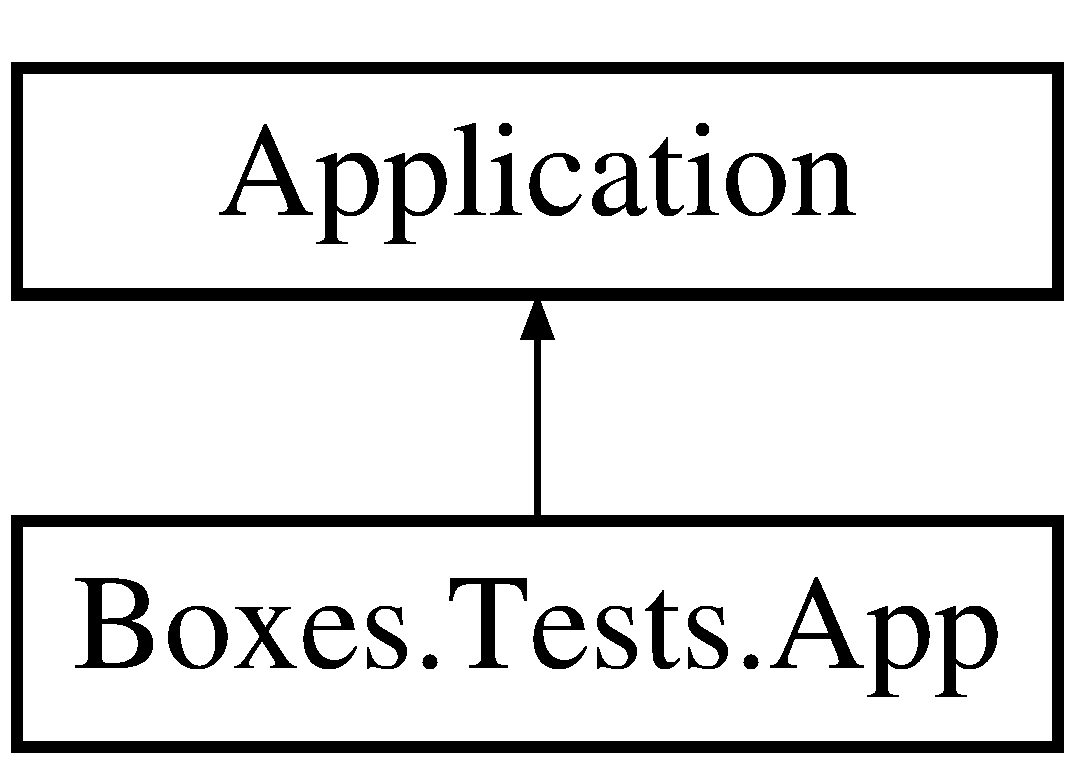
\includegraphics[height=2.000000cm]{class_boxes_1_1_tests_1_1_app}
\end{center}
\end{figure}
\subsection*{Fonctions membres publiques}
\begin{DoxyCompactItemize}
\item 
\hyperlink{class_boxes_1_1_tests_1_1_app_a1999af5186e3e336921b3dc46b9043e8}{App} ()
\begin{DoxyCompactList}\small\item\em Initialise l\textquotesingle{}objet d\textquotesingle{}application de singleton. Il s\textquotesingle{}agit de la première ligne du code créé à être exécutée. Elle correspond donc à l\textquotesingle{}équivalent logique de main() ou Win\+Main(). \end{DoxyCompactList}\end{DoxyCompactItemize}
\subsection*{Fonctions membres protégées}
\begin{DoxyCompactItemize}
\item 
override void \hyperlink{class_boxes_1_1_tests_1_1_app_a3afb9340185c08861e8e4d76d5ea17e0}{On\+Launched} (Launch\+Activated\+Event\+Args e)
\begin{DoxyCompactList}\small\item\em Invoqué lorsque l\textquotesingle{}application est lancée normalement par l\textquotesingle{}utilisateur final. D\textquotesingle{}autres points d\textquotesingle{}entrée seront utilisés par exemple au moment du lancement de l\textquotesingle{}application pour l\textquotesingle{}ouverture d\textquotesingle{}un fichier spécifique. \end{DoxyCompactList}\end{DoxyCompactItemize}
\subsection*{Fonctions membres privées}
\begin{DoxyCompactItemize}
\item 
void \hyperlink{class_boxes_1_1_tests_1_1_app_a5f7bad7719ca5b36161ff193dc2cced0}{On\+Navigation\+Failed} (object sender, Navigation\+Failed\+Event\+Args e)
\begin{DoxyCompactList}\small\item\em Appelé lorsque la navigation vers une page donnée échoue \end{DoxyCompactList}\item 
void \hyperlink{class_boxes_1_1_tests_1_1_app_abb66fa16524f69671eb35df599664463}{On\+Suspending} (object sender, Suspending\+Event\+Args e)
\begin{DoxyCompactList}\small\item\em Appelé lorsque l\textquotesingle{}exécution de l\textquotesingle{}application est suspendue. L\textquotesingle{}état de l\textquotesingle{}application est enregistré sans savoir si l\textquotesingle{}application pourra se fermer ou reprendre sans endommager le contenu de la mémoire. \end{DoxyCompactList}\end{DoxyCompactItemize}


\subsection{Description détaillée}
Fournit un comportement spécifique à l\textquotesingle{}application afin de compléter la classe Application par défaut. 



\subsection{Documentation des constructeurs et destructeur}
\index{Boxes\+::\+Tests\+::\+App@{Boxes\+::\+Tests\+::\+App}!App@{App}}
\index{App@{App}!Boxes\+::\+Tests\+::\+App@{Boxes\+::\+Tests\+::\+App}}
\subsubsection[{\texorpdfstring{App()}{App()}}]{\setlength{\rightskip}{0pt plus 5cm}Boxes.\+Tests.\+App.\+App (
\begin{DoxyParamCaption}
{}
\end{DoxyParamCaption}
)}\hypertarget{class_boxes_1_1_tests_1_1_app_a1999af5186e3e336921b3dc46b9043e8}{}\label{class_boxes_1_1_tests_1_1_app_a1999af5186e3e336921b3dc46b9043e8}


Initialise l\textquotesingle{}objet d\textquotesingle{}application de singleton. Il s\textquotesingle{}agit de la première ligne du code créé à être exécutée. Elle correspond donc à l\textquotesingle{}équivalent logique de main() ou Win\+Main(). 



\subsection{Documentation des fonctions membres}
\index{Boxes\+::\+Tests\+::\+App@{Boxes\+::\+Tests\+::\+App}!On\+Launched@{On\+Launched}}
\index{On\+Launched@{On\+Launched}!Boxes\+::\+Tests\+::\+App@{Boxes\+::\+Tests\+::\+App}}
\subsubsection[{\texorpdfstring{On\+Launched(\+Launch\+Activated\+Event\+Args e)}{OnLaunched(LaunchActivatedEventArgs e)}}]{\setlength{\rightskip}{0pt plus 5cm}override void Boxes.\+Tests.\+App.\+On\+Launched (
\begin{DoxyParamCaption}
\item[{Launch\+Activated\+Event\+Args}]{e}
\end{DoxyParamCaption}
)\hspace{0.3cm}{\ttfamily [protected]}}\hypertarget{class_boxes_1_1_tests_1_1_app_a3afb9340185c08861e8e4d76d5ea17e0}{}\label{class_boxes_1_1_tests_1_1_app_a3afb9340185c08861e8e4d76d5ea17e0}


Invoqué lorsque l\textquotesingle{}application est lancée normalement par l\textquotesingle{}utilisateur final. D\textquotesingle{}autres points d\textquotesingle{}entrée seront utilisés par exemple au moment du lancement de l\textquotesingle{}application pour l\textquotesingle{}ouverture d\textquotesingle{}un fichier spécifique. 


\begin{DoxyParams}{Paramètres}
{\em e} & Détails concernant la requête et le processus de lancement. \\
\hline
\end{DoxyParams}
\index{Boxes\+::\+Tests\+::\+App@{Boxes\+::\+Tests\+::\+App}!On\+Navigation\+Failed@{On\+Navigation\+Failed}}
\index{On\+Navigation\+Failed@{On\+Navigation\+Failed}!Boxes\+::\+Tests\+::\+App@{Boxes\+::\+Tests\+::\+App}}
\subsubsection[{\texorpdfstring{On\+Navigation\+Failed(object sender, Navigation\+Failed\+Event\+Args e)}{OnNavigationFailed(object sender, NavigationFailedEventArgs e)}}]{\setlength{\rightskip}{0pt plus 5cm}void Boxes.\+Tests.\+App.\+On\+Navigation\+Failed (
\begin{DoxyParamCaption}
\item[{object}]{sender, }
\item[{Navigation\+Failed\+Event\+Args}]{e}
\end{DoxyParamCaption}
)\hspace{0.3cm}{\ttfamily [private]}}\hypertarget{class_boxes_1_1_tests_1_1_app_a5f7bad7719ca5b36161ff193dc2cced0}{}\label{class_boxes_1_1_tests_1_1_app_a5f7bad7719ca5b36161ff193dc2cced0}


Appelé lorsque la navigation vers une page donnée échoue 


\begin{DoxyParams}{Paramètres}
{\em sender} & Frame à l\textquotesingle{}origine de l\textquotesingle{}échec de navigation. \\
\hline
{\em e} & Détails relatifs à l\textquotesingle{}échec de navigation. \\
\hline
\end{DoxyParams}
\index{Boxes\+::\+Tests\+::\+App@{Boxes\+::\+Tests\+::\+App}!On\+Suspending@{On\+Suspending}}
\index{On\+Suspending@{On\+Suspending}!Boxes\+::\+Tests\+::\+App@{Boxes\+::\+Tests\+::\+App}}
\subsubsection[{\texorpdfstring{On\+Suspending(object sender, Suspending\+Event\+Args e)}{OnSuspending(object sender, SuspendingEventArgs e)}}]{\setlength{\rightskip}{0pt plus 5cm}void Boxes.\+Tests.\+App.\+On\+Suspending (
\begin{DoxyParamCaption}
\item[{object}]{sender, }
\item[{Suspending\+Event\+Args}]{e}
\end{DoxyParamCaption}
)\hspace{0.3cm}{\ttfamily [private]}}\hypertarget{class_boxes_1_1_tests_1_1_app_abb66fa16524f69671eb35df599664463}{}\label{class_boxes_1_1_tests_1_1_app_abb66fa16524f69671eb35df599664463}


Appelé lorsque l\textquotesingle{}exécution de l\textquotesingle{}application est suspendue. L\textquotesingle{}état de l\textquotesingle{}application est enregistré sans savoir si l\textquotesingle{}application pourra se fermer ou reprendre sans endommager le contenu de la mémoire. 


\begin{DoxyParams}{Paramètres}
{\em sender} & Source de la requête de suspension. \\
\hline
{\em e} & Détails de la requête de suspension. \\
\hline
\end{DoxyParams}


La documentation de cette classe a été générée à partir du fichier suivant \+:\begin{DoxyCompactItemize}
\item 
C\+:/\+Users/thoma/\+One\+Drive/\+Documents/\+Visual Studio 2015/\+Projects/\+Boxes/\+Boxes.\+Tests/\hyperlink{_unit_test_app_8xaml_8cs}{Unit\+Test\+App.\+xaml.\+cs}\end{DoxyCompactItemize}

\hypertarget{class_boxes_1_1_tests_1_1_box_view_model_tests}{}\section{Référence de la classe Boxes.\+Tests.\+Box\+View\+Model\+Tests}
\label{class_boxes_1_1_tests_1_1_box_view_model_tests}\index{Boxes.\+Tests.\+Box\+View\+Model\+Tests@{Boxes.\+Tests.\+Box\+View\+Model\+Tests}}


Effectue les tests unitaires du view model Box\+View\+Model.  


\subsection*{Fonctions membres publiques}
\begin{DoxyCompactItemize}
\item 
void \hyperlink{class_boxes_1_1_tests_1_1_box_view_model_tests_a82cbb0fbb62d965f006597b6dc98ef5b}{Tests\+Initialize} ()
\begin{DoxyCompactList}\small\item\em Effectue les initialisation qui doivent s\textquotesingle{}exécuter avant chaque test. \end{DoxyCompactList}\item 
void \hyperlink{class_boxes_1_1_tests_1_1_box_view_model_tests_ad716bd33ddf90edbcfb65cf961633742}{Tests\+Cleanup} ()
\begin{DoxyCompactList}\small\item\em Effectue les nettoyages de variables devant être faits après l\textquotesingle{}exécution de chaque test. \end{DoxyCompactList}\item 
void \hyperlink{class_boxes_1_1_tests_1_1_box_view_model_tests_a81422a1a1c4e129876ba40889cac29d0}{Initialize\+\_\+\+Box\+As\+Parameter\+\_\+\+Id\+Is\+Box\+Id} ()
\begin{DoxyCompactList}\small\item\em Vérifie que lors de l\textquotesingle{}initialisation du view model, la valeur de la propriété {\ttfamily Id} est la valeur de la propriété {\ttfamily Id} de la boite en paramètre. \end{DoxyCompactList}\item 
void \hyperlink{class_boxes_1_1_tests_1_1_box_view_model_tests_a0adb07f5c44852b09e5e376e10dff44c}{Initialize\+\_\+\+Box\+As\+Parameter\+\_\+\+Title\+Is\+Box\+Title} ()
\begin{DoxyCompactList}\small\item\em Vérifie que lors de l\textquotesingle{}initialisation du view model, la valeur de la propriété {\ttfamily Title} est la valeur de la propriété {\ttfamily Title} de la boite en paramètre. \end{DoxyCompactList}\item 
void \hyperlink{class_boxes_1_1_tests_1_1_box_view_model_tests_a99d787da6ca9aa4158ec0af087079005}{Initialize\+\_\+\+Box\+As\+Parameter\+\_\+\+Description\+Is\+Box\+Description} ()
\begin{DoxyCompactList}\small\item\em Vérifie que lors de l\textquotesingle{}initialisation du view model, la valeur de la propriété {\ttfamily Description} est la valeur de la propriété {\ttfamily Description} de la boite en paramètre. \end{DoxyCompactList}\item 
void \hyperlink{class_boxes_1_1_tests_1_1_box_view_model_tests_a1319ef8f099d7b98af9c97898e6561cb}{Initialize\+\_\+\+Box\+As\+Parameter\+\_\+\+Creator\+Is\+Box\+Creator} ()
\begin{DoxyCompactList}\small\item\em Vérifie que lors de l\textquotesingle{}initialisation du view model, la valeur de la propriété {\ttfamily Creator} est la valeur de la propriété {\ttfamily Creator} de la boite en paramètre. \end{DoxyCompactList}\item 
void \hyperlink{class_boxes_1_1_tests_1_1_box_view_model_tests_a70d8f357605fc5801a7a2be6a3bbb4c9}{Initialize\+\_\+\+User\+Subscribed\+\_\+\+Is\+Subscribed\+True} ()
\begin{DoxyCompactList}\small\item\em Vérifie que lors de l\textquotesingle{}initialisation du view model, si l\textquotesingle{}utilisateur courant est dans la liste des abonnés de la boite, la propriété {\ttfamily Is\+User\+Subscribed} est vraie. \end{DoxyCompactList}\item 
void \hyperlink{class_boxes_1_1_tests_1_1_box_view_model_tests_a65f4c32b8dc0116c21ac2105a045f996}{Initialize\+\_\+\+User\+Not\+Subscribed\+\_\+\+Is\+Subscribed\+False} ()
\begin{DoxyCompactList}\small\item\em Vérifie que lors de l\textquotesingle{}initialisation du view model, si l\textquotesingle{}utilisateur courant n\textquotesingle{}est pas dans la liste des abonnés de la boite, la propriété {\ttfamily Is\+User\+Subscribed} est fausse. \end{DoxyCompactList}\item 
void \hyperlink{class_boxes_1_1_tests_1_1_box_view_model_tests_ac836dee13f611dac60d607624ccc210d}{Initialize\+\_\+\+User\+Is\+Creator\+\_\+\+Is\+User\+Created\+True} ()
\begin{DoxyCompactList}\small\item\em Vérifie que lors de l\textquotesingle{}initialisation du view model, si l\textquotesingle{}utilisateur courant est le créateur de la boite, la propriété {\ttfamily Is\+User\+Created} est vraie. \end{DoxyCompactList}\item 
void \hyperlink{class_boxes_1_1_tests_1_1_box_view_model_tests_a639f3263666d93117b3bdb4471eae602}{Initialize\+\_\+\+User\+Is\+Not\+Creator\+\_\+\+Is\+User\+Created\+False} ()
\begin{DoxyCompactList}\small\item\em Vérifie que lors de l\textquotesingle{}initialisation du view model, si l\textquotesingle{}utilisateur courant n\textquotesingle{}est pas le créateur de la boite, la propriété {\ttfamily Is\+User\+Created} est fausse. \end{DoxyCompactList}\item 
void \hyperlink{class_boxes_1_1_tests_1_1_box_view_model_tests_a5a09aa20411d522fe7d7b6ea18bd8163}{Initialize\+\_\+\+Navigation\+To\+Box\+\_\+\+Is\+Back\+Button\+Visible\+Message\+Sent} ()
\begin{DoxyCompactList}\small\item\em Vérifie que lors de l\textquotesingle{}initialisation du view model, un message de type Is\+Back\+Button\+Visible\+Message est envoyé. \end{DoxyCompactList}\item 
void \hyperlink{class_boxes_1_1_tests_1_1_box_view_model_tests_a93ebcdce7b66d31a8d362c80342904da}{Initialize\+\_\+\+Navigation\+To\+Box\+\_\+\+Shell\+Title\+Message\+Sent} ()
\begin{DoxyCompactList}\small\item\em Vérifie que lors de l\textquotesingle{}initialisation du view model, un message de type Shell\+Title\+Message est envoyé. \end{DoxyCompactList}\item 
async Task \hyperlink{class_boxes_1_1_tests_1_1_box_view_model_tests_aa6bf6381bc58f74e36e61be08ec4d9f7}{Initialize\+\_\+\+Navigation\+To\+Box\+\_\+\+Posts\+Not\+Empty} ()
\begin{DoxyCompactList}\small\item\em Vérifie que lors de l\textquotesingle{}initialisation du view model, la liste des posts de la boite n\textquotesingle{}est pas vide. \end{DoxyCompactList}\item 
void \hyperlink{class_boxes_1_1_tests_1_1_box_view_model_tests_a509fef9ab5036f8523007bb793262f6d}{Cleanup\+\_\+\+Navigation\+From\+Box\+\_\+\+Is\+Back\+Button\+Visible\+Message\+Sent} ()
\begin{DoxyCompactList}\small\item\em Vérifie que lorsque l\textquotesingle{}utilisateur quitte la page, un message de type Is\+Back\+Button\+Visible\+Message est envoyé. \end{DoxyCompactList}\item 
void \hyperlink{class_boxes_1_1_tests_1_1_box_view_model_tests_ace920ab76de14f39da3c4fe16033419f}{Post\+Command\+\_\+\+Go\+To\+Post\+Page\+\_\+\+Current\+Page\+Is\+Post} ()
\begin{DoxyCompactList}\small\item\em Vérifie que lorsque l\textquotesingle{}utilisateur souhaite voir le détail d\textquotesingle{}un post et qu\textquotesingle{}il fait appel à la commande d\textquotesingle{}affichage d\textquotesingle{}un post, la page actuellement affichée est bien celle du post. \end{DoxyCompactList}\item 
void \hyperlink{class_boxes_1_1_tests_1_1_box_view_model_tests_a1de62d7f0aba07485744808f5b45713d}{Post\+Command\+\_\+\+Go\+To\+Post\+Page\+\_\+\+Current\+Page\+Parameter\+Is\+Post\+To\+Show} ()
\begin{DoxyCompactList}\small\item\em Vérifie que lorsque l\textquotesingle{}utilisateur souhaite voir le détail d\textquotesingle{}un post et qu\textquotesingle{}il fait appel à la commande d\textquotesingle{}affichage de ce post, le paramètre transmis à la page actuellement affichée est bien le post en paramètre. \end{DoxyCompactList}\item 
void \hyperlink{class_boxes_1_1_tests_1_1_box_view_model_tests_a5f955c1e3b22af4d7f87fad58fd5c22e}{Create\+Post\+Command\+\_\+\+Post\+Content\+Is\+Null\+Or\+White\+Space\+\_\+\+Cannot\+Execute} (string post\+Content)
\begin{DoxyCompactList}\small\item\em Vérifie que lorsque la commande de création d\textquotesingle{}un post est appelée et que le contenu du post à créer est vide (ou succession d\textquotesingle{}espaces), cette dernière ne peut s\textquotesingle{}exécuter. \end{DoxyCompactList}\item 
void \hyperlink{class_boxes_1_1_tests_1_1_box_view_model_tests_ac8700b19dd4b9da34ece813cc0a3315e}{Create\+Post\+Command\+\_\+\+Is\+Posting\+\_\+\+Cannot\+Execute} ()
\begin{DoxyCompactList}\small\item\em Vérifie que lorsqu\textquotesingle{}un post est en cours de création, la commande de création d\textquotesingle{}un post ne peut s\textquotesingle{}exécuter. \end{DoxyCompactList}\item 
void \hyperlink{class_boxes_1_1_tests_1_1_box_view_model_tests_a2ef7775cc88a525befef1e603fb84bbd}{Create\+Post\+Command\+\_\+\+Is\+Not\+Posting\+Content\+Not\+Null\+Or\+White\+Space\+\_\+\+Can\+Execute} ()
\begin{DoxyCompactList}\small\item\em Vérifie que lorsque la commande de création d\textquotesingle{}un post est appelée, que le contenu du post à créer n\textquotesingle{}est pas vide (ou succession d\textquotesingle{}espaces) et qu\textquotesingle{}aucun post n\textquotesingle{}est en cours de création, la commande de création peut s\textquotesingle{}exécuter. \end{DoxyCompactList}\item 
void \hyperlink{class_boxes_1_1_tests_1_1_box_view_model_tests_abca3833cda01ac0726f8651c87d1f5cb}{Create\+Post\+Command\+\_\+\+Valid\+Data\+\_\+\+Post\+Created} ()
\begin{DoxyCompactList}\small\item\em Vérifie que lorsque la commande de création d\textquotesingle{}un post est appelée avec des données valides, le post est bien créé. \end{DoxyCompactList}\item 
void \hyperlink{class_boxes_1_1_tests_1_1_box_view_model_tests_a69b701c72f976a0b9991a68c32ebb1f6}{Create\+Post\+Command\+\_\+\+Valid\+Data\+\_\+\+Posts\+Not\+Empty} ()
\begin{DoxyCompactList}\small\item\em Vérifie que lorsque la commande de création d\textquotesingle{}un post est appelée avec des données valides, le post créé est bien ajouté dans la liste {\ttfamily Posts} du view model. \end{DoxyCompactList}\item 
void \hyperlink{class_boxes_1_1_tests_1_1_box_view_model_tests_a15cda1891327ab478a31afd8ef210945}{Subscribe\+Command\+\_\+\+Is\+Subscribing\+\_\+\+Cannot\+Execute} ()
\begin{DoxyCompactList}\small\item\em Vérifie que lorsqu\textquotesingle{}un abonnement est en cours, la commande d\textquotesingle{}abonnement ne peut s\textquotesingle{}exécuter. \end{DoxyCompactList}\item 
void \hyperlink{class_boxes_1_1_tests_1_1_box_view_model_tests_a8d845723caa18ff42634cbd9c1c22ebd}{Subscribe\+Command\+\_\+\+Is\+Not\+Subscribing\+\_\+\+Can\+Execute} ()
\begin{DoxyCompactList}\small\item\em Vérifie que lorsqu\textquotesingle{}aucun abonnement n\textquotesingle{}est en cours, la commande d\textquotesingle{}abonnement peut s\textquotesingle{}exécuter. \end{DoxyCompactList}\item 
async Task \hyperlink{class_boxes_1_1_tests_1_1_box_view_model_tests_ac2204a12057fc542c3c74c7da7e25c17}{Subscribe\+Command\+\_\+\+User\+Not\+Subscribed\+\_\+\+User\+Attached\+To\+Box} ()
\begin{DoxyCompactList}\small\item\em Vérifie que lorsque la commande d\textquotesingle{}abonnement est appelée, l\textquotesingle{}utilisateur courant est bien rattaché à la boite. \end{DoxyCompactList}\item 
async Task \hyperlink{class_boxes_1_1_tests_1_1_box_view_model_tests_af36908333befbb932ae89f68be588321}{Subscribe\+Command\+\_\+\+User\+Not\+Subscribed\+\_\+\+Is\+User\+Subscribed\+True} ()
\begin{DoxyCompactList}\small\item\em Vérifie que lorsque la commande d\textquotesingle{}abonnement est appelée, la valeur de la propriété {\ttfamily Is\+User\+Subscribed} du view model est bien à true. \end{DoxyCompactList}\item 
void \hyperlink{class_boxes_1_1_tests_1_1_box_view_model_tests_ae78dc71e8f88759e814546559bd34ee0}{Unsubscribe\+Command\+\_\+\+Is\+Unsubscribing\+\_\+\+Cannot\+Execute} ()
\begin{DoxyCompactList}\small\item\em Vérifie que lorsqu\textquotesingle{}un désabonnement est en cours, la commande de désabonnement ne peut s\textquotesingle{}exécuter. \end{DoxyCompactList}\item 
void \hyperlink{class_boxes_1_1_tests_1_1_box_view_model_tests_a4083ed75efa10a2454d99875dbefa852}{Unsubscribe\+Command\+\_\+\+Is\+Not\+Unsubscribing\+\_\+\+Can\+Execute} ()
\begin{DoxyCompactList}\small\item\em Vérifie que lorsqu\textquotesingle{}aucun désabonnement n\textquotesingle{}est en cours, la commande de désabonnement peut s\textquotesingle{}exécuter. \end{DoxyCompactList}\item 
async Task \hyperlink{class_boxes_1_1_tests_1_1_box_view_model_tests_a8a989a46d267eedaa9f31b70f47e4758}{Unsubscribe\+Command\+\_\+\+User\+Subscribed\+\_\+\+User\+Detached\+From\+Box} ()
\begin{DoxyCompactList}\small\item\em Vérifie que lorsque la commande de désabonnement est appelée, l\textquotesingle{}utilisateur courant n\textquotesingle{}est plus rattaché à la boite. \end{DoxyCompactList}\item 
async Task \hyperlink{class_boxes_1_1_tests_1_1_box_view_model_tests_ac02012cebfd38a0e20ccf51e47139efa}{Unsubscribe\+Command\+\_\+\+User\+Subscribed\+\_\+\+Is\+User\+Subscribed\+False} ()
\begin{DoxyCompactList}\small\item\em Vérifie que lorsque la commande de désabonnement est appelée, la valeur de la propriété {\ttfamily Is\+User\+Subscribed} du view model est à false. \end{DoxyCompactList}\item 
void \hyperlink{class_boxes_1_1_tests_1_1_box_view_model_tests_aa359ecc689414c8a78edac5188f935e5}{Show\+Edit\+Box\+Command\+\_\+\+Go\+To\+Edit\+Box\+\_\+\+Current\+Page\+Is\+Edit\+Box} ()
\begin{DoxyCompactList}\small\item\em Vérifie que lorsque la commande d\textquotesingle{}affichage de la page d\textquotesingle{}édition d\textquotesingle{}une boite est appelée, la page actuellement affichée est la page d\textquotesingle{}édition d\textquotesingle{}une boite. \end{DoxyCompactList}\item 
void \hyperlink{class_boxes_1_1_tests_1_1_box_view_model_tests_a5f6645029f13067e1875471a7395bc51}{Show\+Edit\+Box\+Command\+\_\+\+Go\+To\+Edit\+Box\+\_\+\+Current\+Page\+Parameter\+Is\+Box\+To\+Edit} ()
\begin{DoxyCompactList}\small\item\em Vérifie que lorsque la commande d\textquotesingle{}affichage de la page d\textquotesingle{}édition d\textquotesingle{}une boite est appelée, le paramètre transmis à la page actuellement affichée est bien la boite à modifier. \end{DoxyCompactList}\item 
void \hyperlink{class_boxes_1_1_tests_1_1_box_view_model_tests_a23a9d2873344050b8f4036dc6a1650d0}{Delete\+Box\+Command\+\_\+\+Is\+Deleting\+\_\+\+Cannot\+Execute} ()
\begin{DoxyCompactList}\small\item\em Vérifie que la commande de suppression ne peut s\textquotesingle{}exécuter lorsque la suppression est déjà en cours. \end{DoxyCompactList}\item 
void \hyperlink{class_boxes_1_1_tests_1_1_box_view_model_tests_aec861138c7c2e4c11de116228d90cf0a}{Delete\+Box\+Command\+\_\+\+Is\+Not\+Deleting\+\_\+\+Can\+Execute} ()
\begin{DoxyCompactList}\small\item\em Vérifie que la commande de suppression peut s\textquotesingle{}exécuter lorsqu\textquotesingle{}aucune suppression n\textquotesingle{}est en cours. \end{DoxyCompactList}\item 
async Task \hyperlink{class_boxes_1_1_tests_1_1_box_view_model_tests_ae8c8c354b08b87f88851135931073a38}{Delete\+Box\+Command\+\_\+\+User\+Is\+Creator\+\_\+\+Box\+Deleted} ()
\begin{DoxyCompactList}\small\item\em Vérifie que lorsque la commande de suppression est appelée, la boite est bien supprimée. \end{DoxyCompactList}\item 
void \hyperlink{class_boxes_1_1_tests_1_1_box_view_model_tests_a1d4c1b2de83319d31d50bdc9009481c7}{Delete\+Box\+Command\+\_\+\+User\+Is\+Creator\+\_\+\+Current\+Page\+Is\+Root\+Page} ()
\begin{DoxyCompactList}\small\item\em Vérifie que lorsque la commande de suppression est appelée, la page actuellement affichée est la page précédente. \end{DoxyCompactList}\end{DoxyCompactItemize}
\subsection*{Fonctions membres publiques statiques}
\begin{DoxyCompactItemize}
\item 
static void \hyperlink{class_boxes_1_1_tests_1_1_box_view_model_tests_add83da1c10eae5053a4d42da70a790dc}{Class\+Initialize} (Test\+Context context)
\begin{DoxyCompactList}\small\item\em Effectue les initialisation qui doivent être faites avant l\textquotesingle{}exécution du premier test. \end{DoxyCompactList}\item 
static void \hyperlink{class_boxes_1_1_tests_1_1_box_view_model_tests_a444b18fec69689fe0066151b0b60e283}{Class\+Cleanup} ()
\begin{DoxyCompactList}\small\item\em Effectue les nettoyages qui doivent être faits après l\textquotesingle{}exécution du dernier test. \end{DoxyCompactList}\end{DoxyCompactItemize}
\subsection*{Attributs privés}
\begin{DoxyCompactItemize}
\item 
\hyperlink{class_boxes_1_1_tests_1_1_mock_1_1_services_1_1_fake_post_service}{Fake\+Post\+Service} \hyperlink{class_boxes_1_1_tests_1_1_box_view_model_tests_a829b9b859b727182afb2eb3a427c030a}{post\+Service}
\begin{DoxyCompactList}\small\item\em Stock le service d\textquotesingle{}accès aux données fictives de l\textquotesingle{}entité Post. \end{DoxyCompactList}\item 
\hyperlink{class_boxes_1_1_tests_1_1_mock_1_1_services_1_1_fake_box_service}{Fake\+Box\+Service} \hyperlink{class_boxes_1_1_tests_1_1_box_view_model_tests_a04618b94ae1c36e1d89ad38cb10ae7e9}{box\+Service}
\begin{DoxyCompactList}\small\item\em Stock le service d\textquotesingle{}accès aux données fictives de l\textquotesingle{}entité Box. \end{DoxyCompactList}\item 
\hyperlink{class_boxes_1_1_tests_1_1_mock_1_1_services_1_1_fake_navigation_service}{Fake\+Navigation\+Service} \hyperlink{class_boxes_1_1_tests_1_1_box_view_model_tests_a688092cd2b39fbcb90a09c21a30d5330}{navigation\+Service}
\begin{DoxyCompactList}\small\item\em Stock le service de navigation fictif. \end{DoxyCompactList}\item 
\hyperlink{class_boxes_1_1_tests_1_1_mock_1_1_services_1_1_fake_storage_service}{Fake\+Storage\+Service} \hyperlink{class_boxes_1_1_tests_1_1_box_view_model_tests_a3abe073002190161d00e791a25d22f32}{storage\+Service}
\begin{DoxyCompactList}\small\item\em Stock le service d\textquotesingle{}accès aux données fictives de stockage local. \end{DoxyCompactList}\item 
Box\+View\+Model \hyperlink{class_boxes_1_1_tests_1_1_box_view_model_tests_a551e212c039c5d0ae2356c19ec49ed34}{box\+View\+Model}
\begin{DoxyCompactList}\small\item\em Stock le view model de la page d\textquotesingle{}une boite (ici le view model à tester). \end{DoxyCompactList}\end{DoxyCompactItemize}
\subsection*{Attributs privés statiques}
\begin{DoxyCompactItemize}
\item 
static Random \hyperlink{class_boxes_1_1_tests_1_1_box_view_model_tests_a512de1d0123a965a06039b4cf2bd5f40}{random}
\begin{DoxyCompactList}\small\item\em Stock l\textquotesingle{}objet de génération de nombres aléatoires. \end{DoxyCompactList}\end{DoxyCompactItemize}


\subsection{Description détaillée}
Effectue les tests unitaires du view model Box\+View\+Model. 



\subsection{Documentation des fonctions membres}
\index{Boxes\+::\+Tests\+::\+Box\+View\+Model\+Tests@{Boxes\+::\+Tests\+::\+Box\+View\+Model\+Tests}!Class\+Cleanup@{Class\+Cleanup}}
\index{Class\+Cleanup@{Class\+Cleanup}!Boxes\+::\+Tests\+::\+Box\+View\+Model\+Tests@{Boxes\+::\+Tests\+::\+Box\+View\+Model\+Tests}}
\subsubsection[{\texorpdfstring{Class\+Cleanup()}{ClassCleanup()}}]{\setlength{\rightskip}{0pt plus 5cm}static void Boxes.\+Tests.\+Box\+View\+Model\+Tests.\+Class\+Cleanup (
\begin{DoxyParamCaption}
{}
\end{DoxyParamCaption}
)\hspace{0.3cm}{\ttfamily [static]}}\hypertarget{class_boxes_1_1_tests_1_1_box_view_model_tests_a444b18fec69689fe0066151b0b60e283}{}\label{class_boxes_1_1_tests_1_1_box_view_model_tests_a444b18fec69689fe0066151b0b60e283}


Effectue les nettoyages qui doivent être faits après l\textquotesingle{}exécution du dernier test. 

\index{Boxes\+::\+Tests\+::\+Box\+View\+Model\+Tests@{Boxes\+::\+Tests\+::\+Box\+View\+Model\+Tests}!Class\+Initialize@{Class\+Initialize}}
\index{Class\+Initialize@{Class\+Initialize}!Boxes\+::\+Tests\+::\+Box\+View\+Model\+Tests@{Boxes\+::\+Tests\+::\+Box\+View\+Model\+Tests}}
\subsubsection[{\texorpdfstring{Class\+Initialize(\+Test\+Context context)}{ClassInitialize(TestContext context)}}]{\setlength{\rightskip}{0pt plus 5cm}static void Boxes.\+Tests.\+Box\+View\+Model\+Tests.\+Class\+Initialize (
\begin{DoxyParamCaption}
\item[{Test\+Context}]{context}
\end{DoxyParamCaption}
)\hspace{0.3cm}{\ttfamily [static]}}\hypertarget{class_boxes_1_1_tests_1_1_box_view_model_tests_add83da1c10eae5053a4d42da70a790dc}{}\label{class_boxes_1_1_tests_1_1_box_view_model_tests_add83da1c10eae5053a4d42da70a790dc}


Effectue les initialisation qui doivent être faites avant l\textquotesingle{}exécution du premier test. 

\index{Boxes\+::\+Tests\+::\+Box\+View\+Model\+Tests@{Boxes\+::\+Tests\+::\+Box\+View\+Model\+Tests}!Cleanup\+\_\+\+Navigation\+From\+Box\+\_\+\+Is\+Back\+Button\+Visible\+Message\+Sent@{Cleanup\+\_\+\+Navigation\+From\+Box\+\_\+\+Is\+Back\+Button\+Visible\+Message\+Sent}}
\index{Cleanup\+\_\+\+Navigation\+From\+Box\+\_\+\+Is\+Back\+Button\+Visible\+Message\+Sent@{Cleanup\+\_\+\+Navigation\+From\+Box\+\_\+\+Is\+Back\+Button\+Visible\+Message\+Sent}!Boxes\+::\+Tests\+::\+Box\+View\+Model\+Tests@{Boxes\+::\+Tests\+::\+Box\+View\+Model\+Tests}}
\subsubsection[{\texorpdfstring{Cleanup\+\_\+\+Navigation\+From\+Box\+\_\+\+Is\+Back\+Button\+Visible\+Message\+Sent()}{Cleanup_NavigationFromBox_IsBackButtonVisibleMessageSent()}}]{\setlength{\rightskip}{0pt plus 5cm}void Boxes.\+Tests.\+Box\+View\+Model\+Tests.\+Cleanup\+\_\+\+Navigation\+From\+Box\+\_\+\+Is\+Back\+Button\+Visible\+Message\+Sent (
\begin{DoxyParamCaption}
{}
\end{DoxyParamCaption}
)}\hypertarget{class_boxes_1_1_tests_1_1_box_view_model_tests_a509fef9ab5036f8523007bb793262f6d}{}\label{class_boxes_1_1_tests_1_1_box_view_model_tests_a509fef9ab5036f8523007bb793262f6d}


Vérifie que lorsque l\textquotesingle{}utilisateur quitte la page, un message de type Is\+Back\+Button\+Visible\+Message est envoyé. 

\index{Boxes\+::\+Tests\+::\+Box\+View\+Model\+Tests@{Boxes\+::\+Tests\+::\+Box\+View\+Model\+Tests}!Create\+Post\+Command\+\_\+\+Is\+Not\+Posting\+Content\+Not\+Null\+Or\+White\+Space\+\_\+\+Can\+Execute@{Create\+Post\+Command\+\_\+\+Is\+Not\+Posting\+Content\+Not\+Null\+Or\+White\+Space\+\_\+\+Can\+Execute}}
\index{Create\+Post\+Command\+\_\+\+Is\+Not\+Posting\+Content\+Not\+Null\+Or\+White\+Space\+\_\+\+Can\+Execute@{Create\+Post\+Command\+\_\+\+Is\+Not\+Posting\+Content\+Not\+Null\+Or\+White\+Space\+\_\+\+Can\+Execute}!Boxes\+::\+Tests\+::\+Box\+View\+Model\+Tests@{Boxes\+::\+Tests\+::\+Box\+View\+Model\+Tests}}
\subsubsection[{\texorpdfstring{Create\+Post\+Command\+\_\+\+Is\+Not\+Posting\+Content\+Not\+Null\+Or\+White\+Space\+\_\+\+Can\+Execute()}{CreatePostCommand_IsNotPostingContentNotNullOrWhiteSpace_CanExecute()}}]{\setlength{\rightskip}{0pt plus 5cm}void Boxes.\+Tests.\+Box\+View\+Model\+Tests.\+Create\+Post\+Command\+\_\+\+Is\+Not\+Posting\+Content\+Not\+Null\+Or\+White\+Space\+\_\+\+Can\+Execute (
\begin{DoxyParamCaption}
{}
\end{DoxyParamCaption}
)}\hypertarget{class_boxes_1_1_tests_1_1_box_view_model_tests_a2ef7775cc88a525befef1e603fb84bbd}{}\label{class_boxes_1_1_tests_1_1_box_view_model_tests_a2ef7775cc88a525befef1e603fb84bbd}


Vérifie que lorsque la commande de création d\textquotesingle{}un post est appelée, que le contenu du post à créer n\textquotesingle{}est pas vide (ou succession d\textquotesingle{}espaces) et qu\textquotesingle{}aucun post n\textquotesingle{}est en cours de création, la commande de création peut s\textquotesingle{}exécuter. 

\index{Boxes\+::\+Tests\+::\+Box\+View\+Model\+Tests@{Boxes\+::\+Tests\+::\+Box\+View\+Model\+Tests}!Create\+Post\+Command\+\_\+\+Is\+Posting\+\_\+\+Cannot\+Execute@{Create\+Post\+Command\+\_\+\+Is\+Posting\+\_\+\+Cannot\+Execute}}
\index{Create\+Post\+Command\+\_\+\+Is\+Posting\+\_\+\+Cannot\+Execute@{Create\+Post\+Command\+\_\+\+Is\+Posting\+\_\+\+Cannot\+Execute}!Boxes\+::\+Tests\+::\+Box\+View\+Model\+Tests@{Boxes\+::\+Tests\+::\+Box\+View\+Model\+Tests}}
\subsubsection[{\texorpdfstring{Create\+Post\+Command\+\_\+\+Is\+Posting\+\_\+\+Cannot\+Execute()}{CreatePostCommand_IsPosting_CannotExecute()}}]{\setlength{\rightskip}{0pt plus 5cm}void Boxes.\+Tests.\+Box\+View\+Model\+Tests.\+Create\+Post\+Command\+\_\+\+Is\+Posting\+\_\+\+Cannot\+Execute (
\begin{DoxyParamCaption}
{}
\end{DoxyParamCaption}
)}\hypertarget{class_boxes_1_1_tests_1_1_box_view_model_tests_ac8700b19dd4b9da34ece813cc0a3315e}{}\label{class_boxes_1_1_tests_1_1_box_view_model_tests_ac8700b19dd4b9da34ece813cc0a3315e}


Vérifie que lorsqu\textquotesingle{}un post est en cours de création, la commande de création d\textquotesingle{}un post ne peut s\textquotesingle{}exécuter. 

\index{Boxes\+::\+Tests\+::\+Box\+View\+Model\+Tests@{Boxes\+::\+Tests\+::\+Box\+View\+Model\+Tests}!Create\+Post\+Command\+\_\+\+Post\+Content\+Is\+Null\+Or\+White\+Space\+\_\+\+Cannot\+Execute@{Create\+Post\+Command\+\_\+\+Post\+Content\+Is\+Null\+Or\+White\+Space\+\_\+\+Cannot\+Execute}}
\index{Create\+Post\+Command\+\_\+\+Post\+Content\+Is\+Null\+Or\+White\+Space\+\_\+\+Cannot\+Execute@{Create\+Post\+Command\+\_\+\+Post\+Content\+Is\+Null\+Or\+White\+Space\+\_\+\+Cannot\+Execute}!Boxes\+::\+Tests\+::\+Box\+View\+Model\+Tests@{Boxes\+::\+Tests\+::\+Box\+View\+Model\+Tests}}
\subsubsection[{\texorpdfstring{Create\+Post\+Command\+\_\+\+Post\+Content\+Is\+Null\+Or\+White\+Space\+\_\+\+Cannot\+Execute(string post\+Content)}{CreatePostCommand_PostContentIsNullOrWhiteSpace_CannotExecute(string postContent)}}]{\setlength{\rightskip}{0pt plus 5cm}void Boxes.\+Tests.\+Box\+View\+Model\+Tests.\+Create\+Post\+Command\+\_\+\+Post\+Content\+Is\+Null\+Or\+White\+Space\+\_\+\+Cannot\+Execute (
\begin{DoxyParamCaption}
\item[{string}]{post\+Content}
\end{DoxyParamCaption}
)}\hypertarget{class_boxes_1_1_tests_1_1_box_view_model_tests_a5f955c1e3b22af4d7f87fad58fd5c22e}{}\label{class_boxes_1_1_tests_1_1_box_view_model_tests_a5f955c1e3b22af4d7f87fad58fd5c22e}


Vérifie que lorsque la commande de création d\textquotesingle{}un post est appelée et que le contenu du post à créer est vide (ou succession d\textquotesingle{}espaces), cette dernière ne peut s\textquotesingle{}exécuter. 


\begin{DoxyParams}{Paramètres}
{\em post\+Content} & Contenu du post à tester. \\
\hline
\end{DoxyParams}
\index{Boxes\+::\+Tests\+::\+Box\+View\+Model\+Tests@{Boxes\+::\+Tests\+::\+Box\+View\+Model\+Tests}!Create\+Post\+Command\+\_\+\+Valid\+Data\+\_\+\+Post\+Created@{Create\+Post\+Command\+\_\+\+Valid\+Data\+\_\+\+Post\+Created}}
\index{Create\+Post\+Command\+\_\+\+Valid\+Data\+\_\+\+Post\+Created@{Create\+Post\+Command\+\_\+\+Valid\+Data\+\_\+\+Post\+Created}!Boxes\+::\+Tests\+::\+Box\+View\+Model\+Tests@{Boxes\+::\+Tests\+::\+Box\+View\+Model\+Tests}}
\subsubsection[{\texorpdfstring{Create\+Post\+Command\+\_\+\+Valid\+Data\+\_\+\+Post\+Created()}{CreatePostCommand_ValidData_PostCreated()}}]{\setlength{\rightskip}{0pt plus 5cm}void Boxes.\+Tests.\+Box\+View\+Model\+Tests.\+Create\+Post\+Command\+\_\+\+Valid\+Data\+\_\+\+Post\+Created (
\begin{DoxyParamCaption}
{}
\end{DoxyParamCaption}
)}\hypertarget{class_boxes_1_1_tests_1_1_box_view_model_tests_abca3833cda01ac0726f8651c87d1f5cb}{}\label{class_boxes_1_1_tests_1_1_box_view_model_tests_abca3833cda01ac0726f8651c87d1f5cb}


Vérifie que lorsque la commande de création d\textquotesingle{}un post est appelée avec des données valides, le post est bien créé. 

\index{Boxes\+::\+Tests\+::\+Box\+View\+Model\+Tests@{Boxes\+::\+Tests\+::\+Box\+View\+Model\+Tests}!Create\+Post\+Command\+\_\+\+Valid\+Data\+\_\+\+Posts\+Not\+Empty@{Create\+Post\+Command\+\_\+\+Valid\+Data\+\_\+\+Posts\+Not\+Empty}}
\index{Create\+Post\+Command\+\_\+\+Valid\+Data\+\_\+\+Posts\+Not\+Empty@{Create\+Post\+Command\+\_\+\+Valid\+Data\+\_\+\+Posts\+Not\+Empty}!Boxes\+::\+Tests\+::\+Box\+View\+Model\+Tests@{Boxes\+::\+Tests\+::\+Box\+View\+Model\+Tests}}
\subsubsection[{\texorpdfstring{Create\+Post\+Command\+\_\+\+Valid\+Data\+\_\+\+Posts\+Not\+Empty()}{CreatePostCommand_ValidData_PostsNotEmpty()}}]{\setlength{\rightskip}{0pt plus 5cm}void Boxes.\+Tests.\+Box\+View\+Model\+Tests.\+Create\+Post\+Command\+\_\+\+Valid\+Data\+\_\+\+Posts\+Not\+Empty (
\begin{DoxyParamCaption}
{}
\end{DoxyParamCaption}
)}\hypertarget{class_boxes_1_1_tests_1_1_box_view_model_tests_a69b701c72f976a0b9991a68c32ebb1f6}{}\label{class_boxes_1_1_tests_1_1_box_view_model_tests_a69b701c72f976a0b9991a68c32ebb1f6}


Vérifie que lorsque la commande de création d\textquotesingle{}un post est appelée avec des données valides, le post créé est bien ajouté dans la liste {\ttfamily Posts} du view model. 

\index{Boxes\+::\+Tests\+::\+Box\+View\+Model\+Tests@{Boxes\+::\+Tests\+::\+Box\+View\+Model\+Tests}!Delete\+Box\+Command\+\_\+\+Is\+Deleting\+\_\+\+Cannot\+Execute@{Delete\+Box\+Command\+\_\+\+Is\+Deleting\+\_\+\+Cannot\+Execute}}
\index{Delete\+Box\+Command\+\_\+\+Is\+Deleting\+\_\+\+Cannot\+Execute@{Delete\+Box\+Command\+\_\+\+Is\+Deleting\+\_\+\+Cannot\+Execute}!Boxes\+::\+Tests\+::\+Box\+View\+Model\+Tests@{Boxes\+::\+Tests\+::\+Box\+View\+Model\+Tests}}
\subsubsection[{\texorpdfstring{Delete\+Box\+Command\+\_\+\+Is\+Deleting\+\_\+\+Cannot\+Execute()}{DeleteBoxCommand_IsDeleting_CannotExecute()}}]{\setlength{\rightskip}{0pt plus 5cm}void Boxes.\+Tests.\+Box\+View\+Model\+Tests.\+Delete\+Box\+Command\+\_\+\+Is\+Deleting\+\_\+\+Cannot\+Execute (
\begin{DoxyParamCaption}
{}
\end{DoxyParamCaption}
)}\hypertarget{class_boxes_1_1_tests_1_1_box_view_model_tests_a23a9d2873344050b8f4036dc6a1650d0}{}\label{class_boxes_1_1_tests_1_1_box_view_model_tests_a23a9d2873344050b8f4036dc6a1650d0}


Vérifie que la commande de suppression ne peut s\textquotesingle{}exécuter lorsque la suppression est déjà en cours. 

\index{Boxes\+::\+Tests\+::\+Box\+View\+Model\+Tests@{Boxes\+::\+Tests\+::\+Box\+View\+Model\+Tests}!Delete\+Box\+Command\+\_\+\+Is\+Not\+Deleting\+\_\+\+Can\+Execute@{Delete\+Box\+Command\+\_\+\+Is\+Not\+Deleting\+\_\+\+Can\+Execute}}
\index{Delete\+Box\+Command\+\_\+\+Is\+Not\+Deleting\+\_\+\+Can\+Execute@{Delete\+Box\+Command\+\_\+\+Is\+Not\+Deleting\+\_\+\+Can\+Execute}!Boxes\+::\+Tests\+::\+Box\+View\+Model\+Tests@{Boxes\+::\+Tests\+::\+Box\+View\+Model\+Tests}}
\subsubsection[{\texorpdfstring{Delete\+Box\+Command\+\_\+\+Is\+Not\+Deleting\+\_\+\+Can\+Execute()}{DeleteBoxCommand_IsNotDeleting_CanExecute()}}]{\setlength{\rightskip}{0pt plus 5cm}void Boxes.\+Tests.\+Box\+View\+Model\+Tests.\+Delete\+Box\+Command\+\_\+\+Is\+Not\+Deleting\+\_\+\+Can\+Execute (
\begin{DoxyParamCaption}
{}
\end{DoxyParamCaption}
)}\hypertarget{class_boxes_1_1_tests_1_1_box_view_model_tests_aec861138c7c2e4c11de116228d90cf0a}{}\label{class_boxes_1_1_tests_1_1_box_view_model_tests_aec861138c7c2e4c11de116228d90cf0a}


Vérifie que la commande de suppression peut s\textquotesingle{}exécuter lorsqu\textquotesingle{}aucune suppression n\textquotesingle{}est en cours. 

\index{Boxes\+::\+Tests\+::\+Box\+View\+Model\+Tests@{Boxes\+::\+Tests\+::\+Box\+View\+Model\+Tests}!Delete\+Box\+Command\+\_\+\+User\+Is\+Creator\+\_\+\+Box\+Deleted@{Delete\+Box\+Command\+\_\+\+User\+Is\+Creator\+\_\+\+Box\+Deleted}}
\index{Delete\+Box\+Command\+\_\+\+User\+Is\+Creator\+\_\+\+Box\+Deleted@{Delete\+Box\+Command\+\_\+\+User\+Is\+Creator\+\_\+\+Box\+Deleted}!Boxes\+::\+Tests\+::\+Box\+View\+Model\+Tests@{Boxes\+::\+Tests\+::\+Box\+View\+Model\+Tests}}
\subsubsection[{\texorpdfstring{Delete\+Box\+Command\+\_\+\+User\+Is\+Creator\+\_\+\+Box\+Deleted()}{DeleteBoxCommand_UserIsCreator_BoxDeleted()}}]{\setlength{\rightskip}{0pt plus 5cm}async Task Boxes.\+Tests.\+Box\+View\+Model\+Tests.\+Delete\+Box\+Command\+\_\+\+User\+Is\+Creator\+\_\+\+Box\+Deleted (
\begin{DoxyParamCaption}
{}
\end{DoxyParamCaption}
)}\hypertarget{class_boxes_1_1_tests_1_1_box_view_model_tests_ae8c8c354b08b87f88851135931073a38}{}\label{class_boxes_1_1_tests_1_1_box_view_model_tests_ae8c8c354b08b87f88851135931073a38}


Vérifie que lorsque la commande de suppression est appelée, la boite est bien supprimée. 

\index{Boxes\+::\+Tests\+::\+Box\+View\+Model\+Tests@{Boxes\+::\+Tests\+::\+Box\+View\+Model\+Tests}!Delete\+Box\+Command\+\_\+\+User\+Is\+Creator\+\_\+\+Current\+Page\+Is\+Root\+Page@{Delete\+Box\+Command\+\_\+\+User\+Is\+Creator\+\_\+\+Current\+Page\+Is\+Root\+Page}}
\index{Delete\+Box\+Command\+\_\+\+User\+Is\+Creator\+\_\+\+Current\+Page\+Is\+Root\+Page@{Delete\+Box\+Command\+\_\+\+User\+Is\+Creator\+\_\+\+Current\+Page\+Is\+Root\+Page}!Boxes\+::\+Tests\+::\+Box\+View\+Model\+Tests@{Boxes\+::\+Tests\+::\+Box\+View\+Model\+Tests}}
\subsubsection[{\texorpdfstring{Delete\+Box\+Command\+\_\+\+User\+Is\+Creator\+\_\+\+Current\+Page\+Is\+Root\+Page()}{DeleteBoxCommand_UserIsCreator_CurrentPageIsRootPage()}}]{\setlength{\rightskip}{0pt plus 5cm}void Boxes.\+Tests.\+Box\+View\+Model\+Tests.\+Delete\+Box\+Command\+\_\+\+User\+Is\+Creator\+\_\+\+Current\+Page\+Is\+Root\+Page (
\begin{DoxyParamCaption}
{}
\end{DoxyParamCaption}
)}\hypertarget{class_boxes_1_1_tests_1_1_box_view_model_tests_a1d4c1b2de83319d31d50bdc9009481c7}{}\label{class_boxes_1_1_tests_1_1_box_view_model_tests_a1d4c1b2de83319d31d50bdc9009481c7}


Vérifie que lorsque la commande de suppression est appelée, la page actuellement affichée est la page précédente. 

\index{Boxes\+::\+Tests\+::\+Box\+View\+Model\+Tests@{Boxes\+::\+Tests\+::\+Box\+View\+Model\+Tests}!Initialize\+\_\+\+Box\+As\+Parameter\+\_\+\+Creator\+Is\+Box\+Creator@{Initialize\+\_\+\+Box\+As\+Parameter\+\_\+\+Creator\+Is\+Box\+Creator}}
\index{Initialize\+\_\+\+Box\+As\+Parameter\+\_\+\+Creator\+Is\+Box\+Creator@{Initialize\+\_\+\+Box\+As\+Parameter\+\_\+\+Creator\+Is\+Box\+Creator}!Boxes\+::\+Tests\+::\+Box\+View\+Model\+Tests@{Boxes\+::\+Tests\+::\+Box\+View\+Model\+Tests}}
\subsubsection[{\texorpdfstring{Initialize\+\_\+\+Box\+As\+Parameter\+\_\+\+Creator\+Is\+Box\+Creator()}{Initialize_BoxAsParameter_CreatorIsBoxCreator()}}]{\setlength{\rightskip}{0pt plus 5cm}void Boxes.\+Tests.\+Box\+View\+Model\+Tests.\+Initialize\+\_\+\+Box\+As\+Parameter\+\_\+\+Creator\+Is\+Box\+Creator (
\begin{DoxyParamCaption}
{}
\end{DoxyParamCaption}
)}\hypertarget{class_boxes_1_1_tests_1_1_box_view_model_tests_a1319ef8f099d7b98af9c97898e6561cb}{}\label{class_boxes_1_1_tests_1_1_box_view_model_tests_a1319ef8f099d7b98af9c97898e6561cb}


Vérifie que lors de l\textquotesingle{}initialisation du view model, la valeur de la propriété {\ttfamily Creator} est la valeur de la propriété {\ttfamily Creator} de la boite en paramètre. 

\index{Boxes\+::\+Tests\+::\+Box\+View\+Model\+Tests@{Boxes\+::\+Tests\+::\+Box\+View\+Model\+Tests}!Initialize\+\_\+\+Box\+As\+Parameter\+\_\+\+Description\+Is\+Box\+Description@{Initialize\+\_\+\+Box\+As\+Parameter\+\_\+\+Description\+Is\+Box\+Description}}
\index{Initialize\+\_\+\+Box\+As\+Parameter\+\_\+\+Description\+Is\+Box\+Description@{Initialize\+\_\+\+Box\+As\+Parameter\+\_\+\+Description\+Is\+Box\+Description}!Boxes\+::\+Tests\+::\+Box\+View\+Model\+Tests@{Boxes\+::\+Tests\+::\+Box\+View\+Model\+Tests}}
\subsubsection[{\texorpdfstring{Initialize\+\_\+\+Box\+As\+Parameter\+\_\+\+Description\+Is\+Box\+Description()}{Initialize_BoxAsParameter_DescriptionIsBoxDescription()}}]{\setlength{\rightskip}{0pt plus 5cm}void Boxes.\+Tests.\+Box\+View\+Model\+Tests.\+Initialize\+\_\+\+Box\+As\+Parameter\+\_\+\+Description\+Is\+Box\+Description (
\begin{DoxyParamCaption}
{}
\end{DoxyParamCaption}
)}\hypertarget{class_boxes_1_1_tests_1_1_box_view_model_tests_a99d787da6ca9aa4158ec0af087079005}{}\label{class_boxes_1_1_tests_1_1_box_view_model_tests_a99d787da6ca9aa4158ec0af087079005}


Vérifie que lors de l\textquotesingle{}initialisation du view model, la valeur de la propriété {\ttfamily Description} est la valeur de la propriété {\ttfamily Description} de la boite en paramètre. 

\index{Boxes\+::\+Tests\+::\+Box\+View\+Model\+Tests@{Boxes\+::\+Tests\+::\+Box\+View\+Model\+Tests}!Initialize\+\_\+\+Box\+As\+Parameter\+\_\+\+Id\+Is\+Box\+Id@{Initialize\+\_\+\+Box\+As\+Parameter\+\_\+\+Id\+Is\+Box\+Id}}
\index{Initialize\+\_\+\+Box\+As\+Parameter\+\_\+\+Id\+Is\+Box\+Id@{Initialize\+\_\+\+Box\+As\+Parameter\+\_\+\+Id\+Is\+Box\+Id}!Boxes\+::\+Tests\+::\+Box\+View\+Model\+Tests@{Boxes\+::\+Tests\+::\+Box\+View\+Model\+Tests}}
\subsubsection[{\texorpdfstring{Initialize\+\_\+\+Box\+As\+Parameter\+\_\+\+Id\+Is\+Box\+Id()}{Initialize_BoxAsParameter_IdIsBoxId()}}]{\setlength{\rightskip}{0pt plus 5cm}void Boxes.\+Tests.\+Box\+View\+Model\+Tests.\+Initialize\+\_\+\+Box\+As\+Parameter\+\_\+\+Id\+Is\+Box\+Id (
\begin{DoxyParamCaption}
{}
\end{DoxyParamCaption}
)}\hypertarget{class_boxes_1_1_tests_1_1_box_view_model_tests_a81422a1a1c4e129876ba40889cac29d0}{}\label{class_boxes_1_1_tests_1_1_box_view_model_tests_a81422a1a1c4e129876ba40889cac29d0}


Vérifie que lors de l\textquotesingle{}initialisation du view model, la valeur de la propriété {\ttfamily Id} est la valeur de la propriété {\ttfamily Id} de la boite en paramètre. 

\index{Boxes\+::\+Tests\+::\+Box\+View\+Model\+Tests@{Boxes\+::\+Tests\+::\+Box\+View\+Model\+Tests}!Initialize\+\_\+\+Box\+As\+Parameter\+\_\+\+Title\+Is\+Box\+Title@{Initialize\+\_\+\+Box\+As\+Parameter\+\_\+\+Title\+Is\+Box\+Title}}
\index{Initialize\+\_\+\+Box\+As\+Parameter\+\_\+\+Title\+Is\+Box\+Title@{Initialize\+\_\+\+Box\+As\+Parameter\+\_\+\+Title\+Is\+Box\+Title}!Boxes\+::\+Tests\+::\+Box\+View\+Model\+Tests@{Boxes\+::\+Tests\+::\+Box\+View\+Model\+Tests}}
\subsubsection[{\texorpdfstring{Initialize\+\_\+\+Box\+As\+Parameter\+\_\+\+Title\+Is\+Box\+Title()}{Initialize_BoxAsParameter_TitleIsBoxTitle()}}]{\setlength{\rightskip}{0pt plus 5cm}void Boxes.\+Tests.\+Box\+View\+Model\+Tests.\+Initialize\+\_\+\+Box\+As\+Parameter\+\_\+\+Title\+Is\+Box\+Title (
\begin{DoxyParamCaption}
{}
\end{DoxyParamCaption}
)}\hypertarget{class_boxes_1_1_tests_1_1_box_view_model_tests_a0adb07f5c44852b09e5e376e10dff44c}{}\label{class_boxes_1_1_tests_1_1_box_view_model_tests_a0adb07f5c44852b09e5e376e10dff44c}


Vérifie que lors de l\textquotesingle{}initialisation du view model, la valeur de la propriété {\ttfamily Title} est la valeur de la propriété {\ttfamily Title} de la boite en paramètre. 

\index{Boxes\+::\+Tests\+::\+Box\+View\+Model\+Tests@{Boxes\+::\+Tests\+::\+Box\+View\+Model\+Tests}!Initialize\+\_\+\+Navigation\+To\+Box\+\_\+\+Is\+Back\+Button\+Visible\+Message\+Sent@{Initialize\+\_\+\+Navigation\+To\+Box\+\_\+\+Is\+Back\+Button\+Visible\+Message\+Sent}}
\index{Initialize\+\_\+\+Navigation\+To\+Box\+\_\+\+Is\+Back\+Button\+Visible\+Message\+Sent@{Initialize\+\_\+\+Navigation\+To\+Box\+\_\+\+Is\+Back\+Button\+Visible\+Message\+Sent}!Boxes\+::\+Tests\+::\+Box\+View\+Model\+Tests@{Boxes\+::\+Tests\+::\+Box\+View\+Model\+Tests}}
\subsubsection[{\texorpdfstring{Initialize\+\_\+\+Navigation\+To\+Box\+\_\+\+Is\+Back\+Button\+Visible\+Message\+Sent()}{Initialize_NavigationToBox_IsBackButtonVisibleMessageSent()}}]{\setlength{\rightskip}{0pt plus 5cm}void Boxes.\+Tests.\+Box\+View\+Model\+Tests.\+Initialize\+\_\+\+Navigation\+To\+Box\+\_\+\+Is\+Back\+Button\+Visible\+Message\+Sent (
\begin{DoxyParamCaption}
{}
\end{DoxyParamCaption}
)}\hypertarget{class_boxes_1_1_tests_1_1_box_view_model_tests_a5a09aa20411d522fe7d7b6ea18bd8163}{}\label{class_boxes_1_1_tests_1_1_box_view_model_tests_a5a09aa20411d522fe7d7b6ea18bd8163}


Vérifie que lors de l\textquotesingle{}initialisation du view model, un message de type Is\+Back\+Button\+Visible\+Message est envoyé. 

\index{Boxes\+::\+Tests\+::\+Box\+View\+Model\+Tests@{Boxes\+::\+Tests\+::\+Box\+View\+Model\+Tests}!Initialize\+\_\+\+Navigation\+To\+Box\+\_\+\+Posts\+Not\+Empty@{Initialize\+\_\+\+Navigation\+To\+Box\+\_\+\+Posts\+Not\+Empty}}
\index{Initialize\+\_\+\+Navigation\+To\+Box\+\_\+\+Posts\+Not\+Empty@{Initialize\+\_\+\+Navigation\+To\+Box\+\_\+\+Posts\+Not\+Empty}!Boxes\+::\+Tests\+::\+Box\+View\+Model\+Tests@{Boxes\+::\+Tests\+::\+Box\+View\+Model\+Tests}}
\subsubsection[{\texorpdfstring{Initialize\+\_\+\+Navigation\+To\+Box\+\_\+\+Posts\+Not\+Empty()}{Initialize_NavigationToBox_PostsNotEmpty()}}]{\setlength{\rightskip}{0pt plus 5cm}async Task Boxes.\+Tests.\+Box\+View\+Model\+Tests.\+Initialize\+\_\+\+Navigation\+To\+Box\+\_\+\+Posts\+Not\+Empty (
\begin{DoxyParamCaption}
{}
\end{DoxyParamCaption}
)}\hypertarget{class_boxes_1_1_tests_1_1_box_view_model_tests_aa6bf6381bc58f74e36e61be08ec4d9f7}{}\label{class_boxes_1_1_tests_1_1_box_view_model_tests_aa6bf6381bc58f74e36e61be08ec4d9f7}


Vérifie que lors de l\textquotesingle{}initialisation du view model, la liste des posts de la boite n\textquotesingle{}est pas vide. 

\index{Boxes\+::\+Tests\+::\+Box\+View\+Model\+Tests@{Boxes\+::\+Tests\+::\+Box\+View\+Model\+Tests}!Initialize\+\_\+\+Navigation\+To\+Box\+\_\+\+Shell\+Title\+Message\+Sent@{Initialize\+\_\+\+Navigation\+To\+Box\+\_\+\+Shell\+Title\+Message\+Sent}}
\index{Initialize\+\_\+\+Navigation\+To\+Box\+\_\+\+Shell\+Title\+Message\+Sent@{Initialize\+\_\+\+Navigation\+To\+Box\+\_\+\+Shell\+Title\+Message\+Sent}!Boxes\+::\+Tests\+::\+Box\+View\+Model\+Tests@{Boxes\+::\+Tests\+::\+Box\+View\+Model\+Tests}}
\subsubsection[{\texorpdfstring{Initialize\+\_\+\+Navigation\+To\+Box\+\_\+\+Shell\+Title\+Message\+Sent()}{Initialize_NavigationToBox_ShellTitleMessageSent()}}]{\setlength{\rightskip}{0pt plus 5cm}void Boxes.\+Tests.\+Box\+View\+Model\+Tests.\+Initialize\+\_\+\+Navigation\+To\+Box\+\_\+\+Shell\+Title\+Message\+Sent (
\begin{DoxyParamCaption}
{}
\end{DoxyParamCaption}
)}\hypertarget{class_boxes_1_1_tests_1_1_box_view_model_tests_a93ebcdce7b66d31a8d362c80342904da}{}\label{class_boxes_1_1_tests_1_1_box_view_model_tests_a93ebcdce7b66d31a8d362c80342904da}


Vérifie que lors de l\textquotesingle{}initialisation du view model, un message de type Shell\+Title\+Message est envoyé. 

\index{Boxes\+::\+Tests\+::\+Box\+View\+Model\+Tests@{Boxes\+::\+Tests\+::\+Box\+View\+Model\+Tests}!Initialize\+\_\+\+User\+Is\+Creator\+\_\+\+Is\+User\+Created\+True@{Initialize\+\_\+\+User\+Is\+Creator\+\_\+\+Is\+User\+Created\+True}}
\index{Initialize\+\_\+\+User\+Is\+Creator\+\_\+\+Is\+User\+Created\+True@{Initialize\+\_\+\+User\+Is\+Creator\+\_\+\+Is\+User\+Created\+True}!Boxes\+::\+Tests\+::\+Box\+View\+Model\+Tests@{Boxes\+::\+Tests\+::\+Box\+View\+Model\+Tests}}
\subsubsection[{\texorpdfstring{Initialize\+\_\+\+User\+Is\+Creator\+\_\+\+Is\+User\+Created\+True()}{Initialize_UserIsCreator_IsUserCreatedTrue()}}]{\setlength{\rightskip}{0pt plus 5cm}void Boxes.\+Tests.\+Box\+View\+Model\+Tests.\+Initialize\+\_\+\+User\+Is\+Creator\+\_\+\+Is\+User\+Created\+True (
\begin{DoxyParamCaption}
{}
\end{DoxyParamCaption}
)}\hypertarget{class_boxes_1_1_tests_1_1_box_view_model_tests_ac836dee13f611dac60d607624ccc210d}{}\label{class_boxes_1_1_tests_1_1_box_view_model_tests_ac836dee13f611dac60d607624ccc210d}


Vérifie que lors de l\textquotesingle{}initialisation du view model, si l\textquotesingle{}utilisateur courant est le créateur de la boite, la propriété {\ttfamily Is\+User\+Created} est vraie. 

\index{Boxes\+::\+Tests\+::\+Box\+View\+Model\+Tests@{Boxes\+::\+Tests\+::\+Box\+View\+Model\+Tests}!Initialize\+\_\+\+User\+Is\+Not\+Creator\+\_\+\+Is\+User\+Created\+False@{Initialize\+\_\+\+User\+Is\+Not\+Creator\+\_\+\+Is\+User\+Created\+False}}
\index{Initialize\+\_\+\+User\+Is\+Not\+Creator\+\_\+\+Is\+User\+Created\+False@{Initialize\+\_\+\+User\+Is\+Not\+Creator\+\_\+\+Is\+User\+Created\+False}!Boxes\+::\+Tests\+::\+Box\+View\+Model\+Tests@{Boxes\+::\+Tests\+::\+Box\+View\+Model\+Tests}}
\subsubsection[{\texorpdfstring{Initialize\+\_\+\+User\+Is\+Not\+Creator\+\_\+\+Is\+User\+Created\+False()}{Initialize_UserIsNotCreator_IsUserCreatedFalse()}}]{\setlength{\rightskip}{0pt plus 5cm}void Boxes.\+Tests.\+Box\+View\+Model\+Tests.\+Initialize\+\_\+\+User\+Is\+Not\+Creator\+\_\+\+Is\+User\+Created\+False (
\begin{DoxyParamCaption}
{}
\end{DoxyParamCaption}
)}\hypertarget{class_boxes_1_1_tests_1_1_box_view_model_tests_a639f3263666d93117b3bdb4471eae602}{}\label{class_boxes_1_1_tests_1_1_box_view_model_tests_a639f3263666d93117b3bdb4471eae602}


Vérifie que lors de l\textquotesingle{}initialisation du view model, si l\textquotesingle{}utilisateur courant n\textquotesingle{}est pas le créateur de la boite, la propriété {\ttfamily Is\+User\+Created} est fausse. 

\index{Boxes\+::\+Tests\+::\+Box\+View\+Model\+Tests@{Boxes\+::\+Tests\+::\+Box\+View\+Model\+Tests}!Initialize\+\_\+\+User\+Not\+Subscribed\+\_\+\+Is\+Subscribed\+False@{Initialize\+\_\+\+User\+Not\+Subscribed\+\_\+\+Is\+Subscribed\+False}}
\index{Initialize\+\_\+\+User\+Not\+Subscribed\+\_\+\+Is\+Subscribed\+False@{Initialize\+\_\+\+User\+Not\+Subscribed\+\_\+\+Is\+Subscribed\+False}!Boxes\+::\+Tests\+::\+Box\+View\+Model\+Tests@{Boxes\+::\+Tests\+::\+Box\+View\+Model\+Tests}}
\subsubsection[{\texorpdfstring{Initialize\+\_\+\+User\+Not\+Subscribed\+\_\+\+Is\+Subscribed\+False()}{Initialize_UserNotSubscribed_IsSubscribedFalse()}}]{\setlength{\rightskip}{0pt plus 5cm}void Boxes.\+Tests.\+Box\+View\+Model\+Tests.\+Initialize\+\_\+\+User\+Not\+Subscribed\+\_\+\+Is\+Subscribed\+False (
\begin{DoxyParamCaption}
{}
\end{DoxyParamCaption}
)}\hypertarget{class_boxes_1_1_tests_1_1_box_view_model_tests_a65f4c32b8dc0116c21ac2105a045f996}{}\label{class_boxes_1_1_tests_1_1_box_view_model_tests_a65f4c32b8dc0116c21ac2105a045f996}


Vérifie que lors de l\textquotesingle{}initialisation du view model, si l\textquotesingle{}utilisateur courant n\textquotesingle{}est pas dans la liste des abonnés de la boite, la propriété {\ttfamily Is\+User\+Subscribed} est fausse. 

\index{Boxes\+::\+Tests\+::\+Box\+View\+Model\+Tests@{Boxes\+::\+Tests\+::\+Box\+View\+Model\+Tests}!Initialize\+\_\+\+User\+Subscribed\+\_\+\+Is\+Subscribed\+True@{Initialize\+\_\+\+User\+Subscribed\+\_\+\+Is\+Subscribed\+True}}
\index{Initialize\+\_\+\+User\+Subscribed\+\_\+\+Is\+Subscribed\+True@{Initialize\+\_\+\+User\+Subscribed\+\_\+\+Is\+Subscribed\+True}!Boxes\+::\+Tests\+::\+Box\+View\+Model\+Tests@{Boxes\+::\+Tests\+::\+Box\+View\+Model\+Tests}}
\subsubsection[{\texorpdfstring{Initialize\+\_\+\+User\+Subscribed\+\_\+\+Is\+Subscribed\+True()}{Initialize_UserSubscribed_IsSubscribedTrue()}}]{\setlength{\rightskip}{0pt plus 5cm}void Boxes.\+Tests.\+Box\+View\+Model\+Tests.\+Initialize\+\_\+\+User\+Subscribed\+\_\+\+Is\+Subscribed\+True (
\begin{DoxyParamCaption}
{}
\end{DoxyParamCaption}
)}\hypertarget{class_boxes_1_1_tests_1_1_box_view_model_tests_a70d8f357605fc5801a7a2be6a3bbb4c9}{}\label{class_boxes_1_1_tests_1_1_box_view_model_tests_a70d8f357605fc5801a7a2be6a3bbb4c9}


Vérifie que lors de l\textquotesingle{}initialisation du view model, si l\textquotesingle{}utilisateur courant est dans la liste des abonnés de la boite, la propriété {\ttfamily Is\+User\+Subscribed} est vraie. 

\index{Boxes\+::\+Tests\+::\+Box\+View\+Model\+Tests@{Boxes\+::\+Tests\+::\+Box\+View\+Model\+Tests}!Post\+Command\+\_\+\+Go\+To\+Post\+Page\+\_\+\+Current\+Page\+Is\+Post@{Post\+Command\+\_\+\+Go\+To\+Post\+Page\+\_\+\+Current\+Page\+Is\+Post}}
\index{Post\+Command\+\_\+\+Go\+To\+Post\+Page\+\_\+\+Current\+Page\+Is\+Post@{Post\+Command\+\_\+\+Go\+To\+Post\+Page\+\_\+\+Current\+Page\+Is\+Post}!Boxes\+::\+Tests\+::\+Box\+View\+Model\+Tests@{Boxes\+::\+Tests\+::\+Box\+View\+Model\+Tests}}
\subsubsection[{\texorpdfstring{Post\+Command\+\_\+\+Go\+To\+Post\+Page\+\_\+\+Current\+Page\+Is\+Post()}{PostCommand_GoToPostPage_CurrentPageIsPost()}}]{\setlength{\rightskip}{0pt plus 5cm}void Boxes.\+Tests.\+Box\+View\+Model\+Tests.\+Post\+Command\+\_\+\+Go\+To\+Post\+Page\+\_\+\+Current\+Page\+Is\+Post (
\begin{DoxyParamCaption}
{}
\end{DoxyParamCaption}
)}\hypertarget{class_boxes_1_1_tests_1_1_box_view_model_tests_ace920ab76de14f39da3c4fe16033419f}{}\label{class_boxes_1_1_tests_1_1_box_view_model_tests_ace920ab76de14f39da3c4fe16033419f}


Vérifie que lorsque l\textquotesingle{}utilisateur souhaite voir le détail d\textquotesingle{}un post et qu\textquotesingle{}il fait appel à la commande d\textquotesingle{}affichage d\textquotesingle{}un post, la page actuellement affichée est bien celle du post. 

\index{Boxes\+::\+Tests\+::\+Box\+View\+Model\+Tests@{Boxes\+::\+Tests\+::\+Box\+View\+Model\+Tests}!Post\+Command\+\_\+\+Go\+To\+Post\+Page\+\_\+\+Current\+Page\+Parameter\+Is\+Post\+To\+Show@{Post\+Command\+\_\+\+Go\+To\+Post\+Page\+\_\+\+Current\+Page\+Parameter\+Is\+Post\+To\+Show}}
\index{Post\+Command\+\_\+\+Go\+To\+Post\+Page\+\_\+\+Current\+Page\+Parameter\+Is\+Post\+To\+Show@{Post\+Command\+\_\+\+Go\+To\+Post\+Page\+\_\+\+Current\+Page\+Parameter\+Is\+Post\+To\+Show}!Boxes\+::\+Tests\+::\+Box\+View\+Model\+Tests@{Boxes\+::\+Tests\+::\+Box\+View\+Model\+Tests}}
\subsubsection[{\texorpdfstring{Post\+Command\+\_\+\+Go\+To\+Post\+Page\+\_\+\+Current\+Page\+Parameter\+Is\+Post\+To\+Show()}{PostCommand_GoToPostPage_CurrentPageParameterIsPostToShow()}}]{\setlength{\rightskip}{0pt plus 5cm}void Boxes.\+Tests.\+Box\+View\+Model\+Tests.\+Post\+Command\+\_\+\+Go\+To\+Post\+Page\+\_\+\+Current\+Page\+Parameter\+Is\+Post\+To\+Show (
\begin{DoxyParamCaption}
{}
\end{DoxyParamCaption}
)}\hypertarget{class_boxes_1_1_tests_1_1_box_view_model_tests_a1de62d7f0aba07485744808f5b45713d}{}\label{class_boxes_1_1_tests_1_1_box_view_model_tests_a1de62d7f0aba07485744808f5b45713d}


Vérifie que lorsque l\textquotesingle{}utilisateur souhaite voir le détail d\textquotesingle{}un post et qu\textquotesingle{}il fait appel à la commande d\textquotesingle{}affichage de ce post, le paramètre transmis à la page actuellement affichée est bien le post en paramètre. 

\index{Boxes\+::\+Tests\+::\+Box\+View\+Model\+Tests@{Boxes\+::\+Tests\+::\+Box\+View\+Model\+Tests}!Show\+Edit\+Box\+Command\+\_\+\+Go\+To\+Edit\+Box\+\_\+\+Current\+Page\+Is\+Edit\+Box@{Show\+Edit\+Box\+Command\+\_\+\+Go\+To\+Edit\+Box\+\_\+\+Current\+Page\+Is\+Edit\+Box}}
\index{Show\+Edit\+Box\+Command\+\_\+\+Go\+To\+Edit\+Box\+\_\+\+Current\+Page\+Is\+Edit\+Box@{Show\+Edit\+Box\+Command\+\_\+\+Go\+To\+Edit\+Box\+\_\+\+Current\+Page\+Is\+Edit\+Box}!Boxes\+::\+Tests\+::\+Box\+View\+Model\+Tests@{Boxes\+::\+Tests\+::\+Box\+View\+Model\+Tests}}
\subsubsection[{\texorpdfstring{Show\+Edit\+Box\+Command\+\_\+\+Go\+To\+Edit\+Box\+\_\+\+Current\+Page\+Is\+Edit\+Box()}{ShowEditBoxCommand_GoToEditBox_CurrentPageIsEditBox()}}]{\setlength{\rightskip}{0pt plus 5cm}void Boxes.\+Tests.\+Box\+View\+Model\+Tests.\+Show\+Edit\+Box\+Command\+\_\+\+Go\+To\+Edit\+Box\+\_\+\+Current\+Page\+Is\+Edit\+Box (
\begin{DoxyParamCaption}
{}
\end{DoxyParamCaption}
)}\hypertarget{class_boxes_1_1_tests_1_1_box_view_model_tests_aa359ecc689414c8a78edac5188f935e5}{}\label{class_boxes_1_1_tests_1_1_box_view_model_tests_aa359ecc689414c8a78edac5188f935e5}


Vérifie que lorsque la commande d\textquotesingle{}affichage de la page d\textquotesingle{}édition d\textquotesingle{}une boite est appelée, la page actuellement affichée est la page d\textquotesingle{}édition d\textquotesingle{}une boite. 

\index{Boxes\+::\+Tests\+::\+Box\+View\+Model\+Tests@{Boxes\+::\+Tests\+::\+Box\+View\+Model\+Tests}!Show\+Edit\+Box\+Command\+\_\+\+Go\+To\+Edit\+Box\+\_\+\+Current\+Page\+Parameter\+Is\+Box\+To\+Edit@{Show\+Edit\+Box\+Command\+\_\+\+Go\+To\+Edit\+Box\+\_\+\+Current\+Page\+Parameter\+Is\+Box\+To\+Edit}}
\index{Show\+Edit\+Box\+Command\+\_\+\+Go\+To\+Edit\+Box\+\_\+\+Current\+Page\+Parameter\+Is\+Box\+To\+Edit@{Show\+Edit\+Box\+Command\+\_\+\+Go\+To\+Edit\+Box\+\_\+\+Current\+Page\+Parameter\+Is\+Box\+To\+Edit}!Boxes\+::\+Tests\+::\+Box\+View\+Model\+Tests@{Boxes\+::\+Tests\+::\+Box\+View\+Model\+Tests}}
\subsubsection[{\texorpdfstring{Show\+Edit\+Box\+Command\+\_\+\+Go\+To\+Edit\+Box\+\_\+\+Current\+Page\+Parameter\+Is\+Box\+To\+Edit()}{ShowEditBoxCommand_GoToEditBox_CurrentPageParameterIsBoxToEdit()}}]{\setlength{\rightskip}{0pt plus 5cm}void Boxes.\+Tests.\+Box\+View\+Model\+Tests.\+Show\+Edit\+Box\+Command\+\_\+\+Go\+To\+Edit\+Box\+\_\+\+Current\+Page\+Parameter\+Is\+Box\+To\+Edit (
\begin{DoxyParamCaption}
{}
\end{DoxyParamCaption}
)}\hypertarget{class_boxes_1_1_tests_1_1_box_view_model_tests_a5f6645029f13067e1875471a7395bc51}{}\label{class_boxes_1_1_tests_1_1_box_view_model_tests_a5f6645029f13067e1875471a7395bc51}


Vérifie que lorsque la commande d\textquotesingle{}affichage de la page d\textquotesingle{}édition d\textquotesingle{}une boite est appelée, le paramètre transmis à la page actuellement affichée est bien la boite à modifier. 

\index{Boxes\+::\+Tests\+::\+Box\+View\+Model\+Tests@{Boxes\+::\+Tests\+::\+Box\+View\+Model\+Tests}!Subscribe\+Command\+\_\+\+Is\+Not\+Subscribing\+\_\+\+Can\+Execute@{Subscribe\+Command\+\_\+\+Is\+Not\+Subscribing\+\_\+\+Can\+Execute}}
\index{Subscribe\+Command\+\_\+\+Is\+Not\+Subscribing\+\_\+\+Can\+Execute@{Subscribe\+Command\+\_\+\+Is\+Not\+Subscribing\+\_\+\+Can\+Execute}!Boxes\+::\+Tests\+::\+Box\+View\+Model\+Tests@{Boxes\+::\+Tests\+::\+Box\+View\+Model\+Tests}}
\subsubsection[{\texorpdfstring{Subscribe\+Command\+\_\+\+Is\+Not\+Subscribing\+\_\+\+Can\+Execute()}{SubscribeCommand_IsNotSubscribing_CanExecute()}}]{\setlength{\rightskip}{0pt plus 5cm}void Boxes.\+Tests.\+Box\+View\+Model\+Tests.\+Subscribe\+Command\+\_\+\+Is\+Not\+Subscribing\+\_\+\+Can\+Execute (
\begin{DoxyParamCaption}
{}
\end{DoxyParamCaption}
)}\hypertarget{class_boxes_1_1_tests_1_1_box_view_model_tests_a8d845723caa18ff42634cbd9c1c22ebd}{}\label{class_boxes_1_1_tests_1_1_box_view_model_tests_a8d845723caa18ff42634cbd9c1c22ebd}


Vérifie que lorsqu\textquotesingle{}aucun abonnement n\textquotesingle{}est en cours, la commande d\textquotesingle{}abonnement peut s\textquotesingle{}exécuter. 

\index{Boxes\+::\+Tests\+::\+Box\+View\+Model\+Tests@{Boxes\+::\+Tests\+::\+Box\+View\+Model\+Tests}!Subscribe\+Command\+\_\+\+Is\+Subscribing\+\_\+\+Cannot\+Execute@{Subscribe\+Command\+\_\+\+Is\+Subscribing\+\_\+\+Cannot\+Execute}}
\index{Subscribe\+Command\+\_\+\+Is\+Subscribing\+\_\+\+Cannot\+Execute@{Subscribe\+Command\+\_\+\+Is\+Subscribing\+\_\+\+Cannot\+Execute}!Boxes\+::\+Tests\+::\+Box\+View\+Model\+Tests@{Boxes\+::\+Tests\+::\+Box\+View\+Model\+Tests}}
\subsubsection[{\texorpdfstring{Subscribe\+Command\+\_\+\+Is\+Subscribing\+\_\+\+Cannot\+Execute()}{SubscribeCommand_IsSubscribing_CannotExecute()}}]{\setlength{\rightskip}{0pt plus 5cm}void Boxes.\+Tests.\+Box\+View\+Model\+Tests.\+Subscribe\+Command\+\_\+\+Is\+Subscribing\+\_\+\+Cannot\+Execute (
\begin{DoxyParamCaption}
{}
\end{DoxyParamCaption}
)}\hypertarget{class_boxes_1_1_tests_1_1_box_view_model_tests_a15cda1891327ab478a31afd8ef210945}{}\label{class_boxes_1_1_tests_1_1_box_view_model_tests_a15cda1891327ab478a31afd8ef210945}


Vérifie que lorsqu\textquotesingle{}un abonnement est en cours, la commande d\textquotesingle{}abonnement ne peut s\textquotesingle{}exécuter. 

\index{Boxes\+::\+Tests\+::\+Box\+View\+Model\+Tests@{Boxes\+::\+Tests\+::\+Box\+View\+Model\+Tests}!Subscribe\+Command\+\_\+\+User\+Not\+Subscribed\+\_\+\+Is\+User\+Subscribed\+True@{Subscribe\+Command\+\_\+\+User\+Not\+Subscribed\+\_\+\+Is\+User\+Subscribed\+True}}
\index{Subscribe\+Command\+\_\+\+User\+Not\+Subscribed\+\_\+\+Is\+User\+Subscribed\+True@{Subscribe\+Command\+\_\+\+User\+Not\+Subscribed\+\_\+\+Is\+User\+Subscribed\+True}!Boxes\+::\+Tests\+::\+Box\+View\+Model\+Tests@{Boxes\+::\+Tests\+::\+Box\+View\+Model\+Tests}}
\subsubsection[{\texorpdfstring{Subscribe\+Command\+\_\+\+User\+Not\+Subscribed\+\_\+\+Is\+User\+Subscribed\+True()}{SubscribeCommand_UserNotSubscribed_IsUserSubscribedTrue()}}]{\setlength{\rightskip}{0pt plus 5cm}async Task Boxes.\+Tests.\+Box\+View\+Model\+Tests.\+Subscribe\+Command\+\_\+\+User\+Not\+Subscribed\+\_\+\+Is\+User\+Subscribed\+True (
\begin{DoxyParamCaption}
{}
\end{DoxyParamCaption}
)}\hypertarget{class_boxes_1_1_tests_1_1_box_view_model_tests_af36908333befbb932ae89f68be588321}{}\label{class_boxes_1_1_tests_1_1_box_view_model_tests_af36908333befbb932ae89f68be588321}


Vérifie que lorsque la commande d\textquotesingle{}abonnement est appelée, la valeur de la propriété {\ttfamily Is\+User\+Subscribed} du view model est bien à true. 

\begin{DoxyReturn}{Renvoie}
Tache asynchrone qui permet d\textquotesingle{}attendre la fin des opérations. 
\end{DoxyReturn}
\index{Boxes\+::\+Tests\+::\+Box\+View\+Model\+Tests@{Boxes\+::\+Tests\+::\+Box\+View\+Model\+Tests}!Subscribe\+Command\+\_\+\+User\+Not\+Subscribed\+\_\+\+User\+Attached\+To\+Box@{Subscribe\+Command\+\_\+\+User\+Not\+Subscribed\+\_\+\+User\+Attached\+To\+Box}}
\index{Subscribe\+Command\+\_\+\+User\+Not\+Subscribed\+\_\+\+User\+Attached\+To\+Box@{Subscribe\+Command\+\_\+\+User\+Not\+Subscribed\+\_\+\+User\+Attached\+To\+Box}!Boxes\+::\+Tests\+::\+Box\+View\+Model\+Tests@{Boxes\+::\+Tests\+::\+Box\+View\+Model\+Tests}}
\subsubsection[{\texorpdfstring{Subscribe\+Command\+\_\+\+User\+Not\+Subscribed\+\_\+\+User\+Attached\+To\+Box()}{SubscribeCommand_UserNotSubscribed_UserAttachedToBox()}}]{\setlength{\rightskip}{0pt plus 5cm}async Task Boxes.\+Tests.\+Box\+View\+Model\+Tests.\+Subscribe\+Command\+\_\+\+User\+Not\+Subscribed\+\_\+\+User\+Attached\+To\+Box (
\begin{DoxyParamCaption}
{}
\end{DoxyParamCaption}
)}\hypertarget{class_boxes_1_1_tests_1_1_box_view_model_tests_ac2204a12057fc542c3c74c7da7e25c17}{}\label{class_boxes_1_1_tests_1_1_box_view_model_tests_ac2204a12057fc542c3c74c7da7e25c17}


Vérifie que lorsque la commande d\textquotesingle{}abonnement est appelée, l\textquotesingle{}utilisateur courant est bien rattaché à la boite. 

\begin{DoxyReturn}{Renvoie}
Tache asynchrone qui permet d\textquotesingle{}attendre la fin des opérations. 
\end{DoxyReturn}
\index{Boxes\+::\+Tests\+::\+Box\+View\+Model\+Tests@{Boxes\+::\+Tests\+::\+Box\+View\+Model\+Tests}!Tests\+Cleanup@{Tests\+Cleanup}}
\index{Tests\+Cleanup@{Tests\+Cleanup}!Boxes\+::\+Tests\+::\+Box\+View\+Model\+Tests@{Boxes\+::\+Tests\+::\+Box\+View\+Model\+Tests}}
\subsubsection[{\texorpdfstring{Tests\+Cleanup()}{TestsCleanup()}}]{\setlength{\rightskip}{0pt plus 5cm}void Boxes.\+Tests.\+Box\+View\+Model\+Tests.\+Tests\+Cleanup (
\begin{DoxyParamCaption}
{}
\end{DoxyParamCaption}
)}\hypertarget{class_boxes_1_1_tests_1_1_box_view_model_tests_ad716bd33ddf90edbcfb65cf961633742}{}\label{class_boxes_1_1_tests_1_1_box_view_model_tests_ad716bd33ddf90edbcfb65cf961633742}


Effectue les nettoyages de variables devant être faits après l\textquotesingle{}exécution de chaque test. 

\index{Boxes\+::\+Tests\+::\+Box\+View\+Model\+Tests@{Boxes\+::\+Tests\+::\+Box\+View\+Model\+Tests}!Tests\+Initialize@{Tests\+Initialize}}
\index{Tests\+Initialize@{Tests\+Initialize}!Boxes\+::\+Tests\+::\+Box\+View\+Model\+Tests@{Boxes\+::\+Tests\+::\+Box\+View\+Model\+Tests}}
\subsubsection[{\texorpdfstring{Tests\+Initialize()}{TestsInitialize()}}]{\setlength{\rightskip}{0pt plus 5cm}void Boxes.\+Tests.\+Box\+View\+Model\+Tests.\+Tests\+Initialize (
\begin{DoxyParamCaption}
{}
\end{DoxyParamCaption}
)}\hypertarget{class_boxes_1_1_tests_1_1_box_view_model_tests_a82cbb0fbb62d965f006597b6dc98ef5b}{}\label{class_boxes_1_1_tests_1_1_box_view_model_tests_a82cbb0fbb62d965f006597b6dc98ef5b}


Effectue les initialisation qui doivent s\textquotesingle{}exécuter avant chaque test. 

\index{Boxes\+::\+Tests\+::\+Box\+View\+Model\+Tests@{Boxes\+::\+Tests\+::\+Box\+View\+Model\+Tests}!Unsubscribe\+Command\+\_\+\+Is\+Not\+Unsubscribing\+\_\+\+Can\+Execute@{Unsubscribe\+Command\+\_\+\+Is\+Not\+Unsubscribing\+\_\+\+Can\+Execute}}
\index{Unsubscribe\+Command\+\_\+\+Is\+Not\+Unsubscribing\+\_\+\+Can\+Execute@{Unsubscribe\+Command\+\_\+\+Is\+Not\+Unsubscribing\+\_\+\+Can\+Execute}!Boxes\+::\+Tests\+::\+Box\+View\+Model\+Tests@{Boxes\+::\+Tests\+::\+Box\+View\+Model\+Tests}}
\subsubsection[{\texorpdfstring{Unsubscribe\+Command\+\_\+\+Is\+Not\+Unsubscribing\+\_\+\+Can\+Execute()}{UnsubscribeCommand_IsNotUnsubscribing_CanExecute()}}]{\setlength{\rightskip}{0pt plus 5cm}void Boxes.\+Tests.\+Box\+View\+Model\+Tests.\+Unsubscribe\+Command\+\_\+\+Is\+Not\+Unsubscribing\+\_\+\+Can\+Execute (
\begin{DoxyParamCaption}
{}
\end{DoxyParamCaption}
)}\hypertarget{class_boxes_1_1_tests_1_1_box_view_model_tests_a4083ed75efa10a2454d99875dbefa852}{}\label{class_boxes_1_1_tests_1_1_box_view_model_tests_a4083ed75efa10a2454d99875dbefa852}


Vérifie que lorsqu\textquotesingle{}aucun désabonnement n\textquotesingle{}est en cours, la commande de désabonnement peut s\textquotesingle{}exécuter. 

\index{Boxes\+::\+Tests\+::\+Box\+View\+Model\+Tests@{Boxes\+::\+Tests\+::\+Box\+View\+Model\+Tests}!Unsubscribe\+Command\+\_\+\+Is\+Unsubscribing\+\_\+\+Cannot\+Execute@{Unsubscribe\+Command\+\_\+\+Is\+Unsubscribing\+\_\+\+Cannot\+Execute}}
\index{Unsubscribe\+Command\+\_\+\+Is\+Unsubscribing\+\_\+\+Cannot\+Execute@{Unsubscribe\+Command\+\_\+\+Is\+Unsubscribing\+\_\+\+Cannot\+Execute}!Boxes\+::\+Tests\+::\+Box\+View\+Model\+Tests@{Boxes\+::\+Tests\+::\+Box\+View\+Model\+Tests}}
\subsubsection[{\texorpdfstring{Unsubscribe\+Command\+\_\+\+Is\+Unsubscribing\+\_\+\+Cannot\+Execute()}{UnsubscribeCommand_IsUnsubscribing_CannotExecute()}}]{\setlength{\rightskip}{0pt plus 5cm}void Boxes.\+Tests.\+Box\+View\+Model\+Tests.\+Unsubscribe\+Command\+\_\+\+Is\+Unsubscribing\+\_\+\+Cannot\+Execute (
\begin{DoxyParamCaption}
{}
\end{DoxyParamCaption}
)}\hypertarget{class_boxes_1_1_tests_1_1_box_view_model_tests_ae78dc71e8f88759e814546559bd34ee0}{}\label{class_boxes_1_1_tests_1_1_box_view_model_tests_ae78dc71e8f88759e814546559bd34ee0}


Vérifie que lorsqu\textquotesingle{}un désabonnement est en cours, la commande de désabonnement ne peut s\textquotesingle{}exécuter. 

\index{Boxes\+::\+Tests\+::\+Box\+View\+Model\+Tests@{Boxes\+::\+Tests\+::\+Box\+View\+Model\+Tests}!Unsubscribe\+Command\+\_\+\+User\+Subscribed\+\_\+\+Is\+User\+Subscribed\+False@{Unsubscribe\+Command\+\_\+\+User\+Subscribed\+\_\+\+Is\+User\+Subscribed\+False}}
\index{Unsubscribe\+Command\+\_\+\+User\+Subscribed\+\_\+\+Is\+User\+Subscribed\+False@{Unsubscribe\+Command\+\_\+\+User\+Subscribed\+\_\+\+Is\+User\+Subscribed\+False}!Boxes\+::\+Tests\+::\+Box\+View\+Model\+Tests@{Boxes\+::\+Tests\+::\+Box\+View\+Model\+Tests}}
\subsubsection[{\texorpdfstring{Unsubscribe\+Command\+\_\+\+User\+Subscribed\+\_\+\+Is\+User\+Subscribed\+False()}{UnsubscribeCommand_UserSubscribed_IsUserSubscribedFalse()}}]{\setlength{\rightskip}{0pt plus 5cm}async Task Boxes.\+Tests.\+Box\+View\+Model\+Tests.\+Unsubscribe\+Command\+\_\+\+User\+Subscribed\+\_\+\+Is\+User\+Subscribed\+False (
\begin{DoxyParamCaption}
{}
\end{DoxyParamCaption}
)}\hypertarget{class_boxes_1_1_tests_1_1_box_view_model_tests_ac02012cebfd38a0e20ccf51e47139efa}{}\label{class_boxes_1_1_tests_1_1_box_view_model_tests_ac02012cebfd38a0e20ccf51e47139efa}


Vérifie que lorsque la commande de désabonnement est appelée, la valeur de la propriété {\ttfamily Is\+User\+Subscribed} du view model est à false. 

\begin{DoxyReturn}{Renvoie}
Tache asynchrone qui permet d\textquotesingle{}attendre la fin des opérations. 
\end{DoxyReturn}
\index{Boxes\+::\+Tests\+::\+Box\+View\+Model\+Tests@{Boxes\+::\+Tests\+::\+Box\+View\+Model\+Tests}!Unsubscribe\+Command\+\_\+\+User\+Subscribed\+\_\+\+User\+Detached\+From\+Box@{Unsubscribe\+Command\+\_\+\+User\+Subscribed\+\_\+\+User\+Detached\+From\+Box}}
\index{Unsubscribe\+Command\+\_\+\+User\+Subscribed\+\_\+\+User\+Detached\+From\+Box@{Unsubscribe\+Command\+\_\+\+User\+Subscribed\+\_\+\+User\+Detached\+From\+Box}!Boxes\+::\+Tests\+::\+Box\+View\+Model\+Tests@{Boxes\+::\+Tests\+::\+Box\+View\+Model\+Tests}}
\subsubsection[{\texorpdfstring{Unsubscribe\+Command\+\_\+\+User\+Subscribed\+\_\+\+User\+Detached\+From\+Box()}{UnsubscribeCommand_UserSubscribed_UserDetachedFromBox()}}]{\setlength{\rightskip}{0pt plus 5cm}async Task Boxes.\+Tests.\+Box\+View\+Model\+Tests.\+Unsubscribe\+Command\+\_\+\+User\+Subscribed\+\_\+\+User\+Detached\+From\+Box (
\begin{DoxyParamCaption}
{}
\end{DoxyParamCaption}
)}\hypertarget{class_boxes_1_1_tests_1_1_box_view_model_tests_a8a989a46d267eedaa9f31b70f47e4758}{}\label{class_boxes_1_1_tests_1_1_box_view_model_tests_a8a989a46d267eedaa9f31b70f47e4758}


Vérifie que lorsque la commande de désabonnement est appelée, l\textquotesingle{}utilisateur courant n\textquotesingle{}est plus rattaché à la boite. 

\begin{DoxyReturn}{Renvoie}
Tache asynchrone qui permet d\textquotesingle{}attendre la fin des opérations. 
\end{DoxyReturn}


\subsection{Documentation des données membres}
\index{Boxes\+::\+Tests\+::\+Box\+View\+Model\+Tests@{Boxes\+::\+Tests\+::\+Box\+View\+Model\+Tests}!box\+Service@{box\+Service}}
\index{box\+Service@{box\+Service}!Boxes\+::\+Tests\+::\+Box\+View\+Model\+Tests@{Boxes\+::\+Tests\+::\+Box\+View\+Model\+Tests}}
\subsubsection[{\texorpdfstring{box\+Service}{boxService}}]{\setlength{\rightskip}{0pt plus 5cm}{\bf Fake\+Box\+Service} Boxes.\+Tests.\+Box\+View\+Model\+Tests.\+box\+Service\hspace{0.3cm}{\ttfamily [private]}}\hypertarget{class_boxes_1_1_tests_1_1_box_view_model_tests_a04618b94ae1c36e1d89ad38cb10ae7e9}{}\label{class_boxes_1_1_tests_1_1_box_view_model_tests_a04618b94ae1c36e1d89ad38cb10ae7e9}


Stock le service d\textquotesingle{}accès aux données fictives de l\textquotesingle{}entité Box. 

\index{Boxes\+::\+Tests\+::\+Box\+View\+Model\+Tests@{Boxes\+::\+Tests\+::\+Box\+View\+Model\+Tests}!box\+View\+Model@{box\+View\+Model}}
\index{box\+View\+Model@{box\+View\+Model}!Boxes\+::\+Tests\+::\+Box\+View\+Model\+Tests@{Boxes\+::\+Tests\+::\+Box\+View\+Model\+Tests}}
\subsubsection[{\texorpdfstring{box\+View\+Model}{boxViewModel}}]{\setlength{\rightskip}{0pt plus 5cm}Box\+View\+Model Boxes.\+Tests.\+Box\+View\+Model\+Tests.\+box\+View\+Model\hspace{0.3cm}{\ttfamily [private]}}\hypertarget{class_boxes_1_1_tests_1_1_box_view_model_tests_a551e212c039c5d0ae2356c19ec49ed34}{}\label{class_boxes_1_1_tests_1_1_box_view_model_tests_a551e212c039c5d0ae2356c19ec49ed34}


Stock le view model de la page d\textquotesingle{}une boite (ici le view model à tester). 

\index{Boxes\+::\+Tests\+::\+Box\+View\+Model\+Tests@{Boxes\+::\+Tests\+::\+Box\+View\+Model\+Tests}!navigation\+Service@{navigation\+Service}}
\index{navigation\+Service@{navigation\+Service}!Boxes\+::\+Tests\+::\+Box\+View\+Model\+Tests@{Boxes\+::\+Tests\+::\+Box\+View\+Model\+Tests}}
\subsubsection[{\texorpdfstring{navigation\+Service}{navigationService}}]{\setlength{\rightskip}{0pt plus 5cm}{\bf Fake\+Navigation\+Service} Boxes.\+Tests.\+Box\+View\+Model\+Tests.\+navigation\+Service\hspace{0.3cm}{\ttfamily [private]}}\hypertarget{class_boxes_1_1_tests_1_1_box_view_model_tests_a688092cd2b39fbcb90a09c21a30d5330}{}\label{class_boxes_1_1_tests_1_1_box_view_model_tests_a688092cd2b39fbcb90a09c21a30d5330}


Stock le service de navigation fictif. 

\index{Boxes\+::\+Tests\+::\+Box\+View\+Model\+Tests@{Boxes\+::\+Tests\+::\+Box\+View\+Model\+Tests}!post\+Service@{post\+Service}}
\index{post\+Service@{post\+Service}!Boxes\+::\+Tests\+::\+Box\+View\+Model\+Tests@{Boxes\+::\+Tests\+::\+Box\+View\+Model\+Tests}}
\subsubsection[{\texorpdfstring{post\+Service}{postService}}]{\setlength{\rightskip}{0pt plus 5cm}{\bf Fake\+Post\+Service} Boxes.\+Tests.\+Box\+View\+Model\+Tests.\+post\+Service\hspace{0.3cm}{\ttfamily [private]}}\hypertarget{class_boxes_1_1_tests_1_1_box_view_model_tests_a829b9b859b727182afb2eb3a427c030a}{}\label{class_boxes_1_1_tests_1_1_box_view_model_tests_a829b9b859b727182afb2eb3a427c030a}


Stock le service d\textquotesingle{}accès aux données fictives de l\textquotesingle{}entité Post. 

\index{Boxes\+::\+Tests\+::\+Box\+View\+Model\+Tests@{Boxes\+::\+Tests\+::\+Box\+View\+Model\+Tests}!random@{random}}
\index{random@{random}!Boxes\+::\+Tests\+::\+Box\+View\+Model\+Tests@{Boxes\+::\+Tests\+::\+Box\+View\+Model\+Tests}}
\subsubsection[{\texorpdfstring{random}{random}}]{\setlength{\rightskip}{0pt plus 5cm}Random Boxes.\+Tests.\+Box\+View\+Model\+Tests.\+random\hspace{0.3cm}{\ttfamily [static]}, {\ttfamily [private]}}\hypertarget{class_boxes_1_1_tests_1_1_box_view_model_tests_a512de1d0123a965a06039b4cf2bd5f40}{}\label{class_boxes_1_1_tests_1_1_box_view_model_tests_a512de1d0123a965a06039b4cf2bd5f40}


Stock l\textquotesingle{}objet de génération de nombres aléatoires. 

\index{Boxes\+::\+Tests\+::\+Box\+View\+Model\+Tests@{Boxes\+::\+Tests\+::\+Box\+View\+Model\+Tests}!storage\+Service@{storage\+Service}}
\index{storage\+Service@{storage\+Service}!Boxes\+::\+Tests\+::\+Box\+View\+Model\+Tests@{Boxes\+::\+Tests\+::\+Box\+View\+Model\+Tests}}
\subsubsection[{\texorpdfstring{storage\+Service}{storageService}}]{\setlength{\rightskip}{0pt plus 5cm}{\bf Fake\+Storage\+Service} Boxes.\+Tests.\+Box\+View\+Model\+Tests.\+storage\+Service\hspace{0.3cm}{\ttfamily [private]}}\hypertarget{class_boxes_1_1_tests_1_1_box_view_model_tests_a3abe073002190161d00e791a25d22f32}{}\label{class_boxes_1_1_tests_1_1_box_view_model_tests_a3abe073002190161d00e791a25d22f32}


Stock le service d\textquotesingle{}accès aux données fictives de stockage local. 



La documentation de cette classe a été générée à partir du fichier suivant \+:\begin{DoxyCompactItemize}
\item 
C\+:/\+Users/thoma/\+One\+Drive/\+Documents/\+Visual Studio 2015/\+Projects/\+Boxes/\+Boxes.\+Tests/\hyperlink{_box_view_model_tests_8cs}{Box\+View\+Model\+Tests.\+cs}\end{DoxyCompactItemize}

\hypertarget{class_boxes_1_1_tests_1_1_create_box_view_model_tests}{}\section{Référence de la classe Boxes.\+Tests.\+Create\+Box\+View\+Model\+Tests}
\label{class_boxes_1_1_tests_1_1_create_box_view_model_tests}\index{Boxes.\+Tests.\+Create\+Box\+View\+Model\+Tests@{Boxes.\+Tests.\+Create\+Box\+View\+Model\+Tests}}


Effectue les tests unitaires concernant le view model Create\+Box\+View\+Model.  


\subsection*{Fonctions membres publiques}
\begin{DoxyCompactItemize}
\item 
void \hyperlink{class_boxes_1_1_tests_1_1_create_box_view_model_tests_a1d813751528e634b253d780fcc794779}{Tests\+Initialize} ()
\begin{DoxyCompactList}\small\item\em Effectue les initialisation qui doivent s\textquotesingle{}exécuter avant chaque test. \end{DoxyCompactList}\item 
void \hyperlink{class_boxes_1_1_tests_1_1_create_box_view_model_tests_a2a692c8de3378e034057910464104f95}{Tests\+Cleanup} ()
\begin{DoxyCompactList}\small\item\em Effectue les nettoyages de variables devant être faits après l\textquotesingle{}exécution de chaque test. \end{DoxyCompactList}\item 
void \hyperlink{class_boxes_1_1_tests_1_1_create_box_view_model_tests_adeb87abdc4260dc20a35f481ae41a976}{Initialize\+\_\+\+Navigation\+To\+Create\+Box\+\_\+\+Is\+Back\+Button\+Visible\+Message\+Sent} ()
\begin{DoxyCompactList}\small\item\em Vérifie si lors de l\textquotesingle{}initialisation du view model, un message de type Is\+Back\+Button\+Visible\+Message est envoyé. \end{DoxyCompactList}\item 
void \hyperlink{class_boxes_1_1_tests_1_1_create_box_view_model_tests_a7211d7dda73fcadf8b1355b9448fab0d}{Initialize\+\_\+\+Navigation\+To\+Create\+Box\+\_\+\+Shell\+Title\+Message\+Sent} ()
\begin{DoxyCompactList}\small\item\em Vérifie si lors de l\textquotesingle{}initialisation du view model, un message de type Shell\+Title\+Message est envoyé. \end{DoxyCompactList}\item 
void \hyperlink{class_boxes_1_1_tests_1_1_create_box_view_model_tests_a6c22cfcf1332b17894e3e60c3ff7961f}{Cleanup\+\_\+\+Navigation\+From\+Create\+Box\+\_\+\+Is\+Back\+Button\+Visible\+Message\+Sent} ()
\begin{DoxyCompactList}\small\item\em Vérifie si lorsque l\textquotesingle{}utilisateur quitte la page de création d\textquotesingle{}une boite, un message de type Is\+Back\+Button\+Visible\+Message est envoyé. \end{DoxyCompactList}\item 
void \hyperlink{class_boxes_1_1_tests_1_1_create_box_view_model_tests_acccc1b16f201142fa8d9a336fd7680f0}{Cleanup\+\_\+\+Navigation\+From\+Create\+Box\+\_\+\+Title\+Is\+Null} ()
\begin{DoxyCompactList}\small\item\em Vérifie que lorsque l\textquotesingle{}utilisateur quitte la page de création d\textquotesingle{}une boite, le champ \char`\"{}\+Titre\char`\"{} est bien vidé. \end{DoxyCompactList}\item 
void \hyperlink{class_boxes_1_1_tests_1_1_create_box_view_model_tests_a1900608827ee7d9726b9a2188b884676}{Cleanup\+\_\+\+Navigation\+From\+Create\+Box\+\_\+\+Description\+Is\+Null} ()
\begin{DoxyCompactList}\small\item\em Vérifie que lorsque l\textquotesingle{}utilisateur quitte la page de création d\textquotesingle{}une boite, le champ \char`\"{}\+Description\char`\"{} est bien vidé. \end{DoxyCompactList}\item 
void \hyperlink{class_boxes_1_1_tests_1_1_create_box_view_model_tests_a132cbc9e8ed6598e75e8edca409c579f}{Create\+Box\+Command\+\_\+\+Is\+Creating\+\_\+\+Cannot\+Execute} ()
\begin{DoxyCompactList}\small\item\em Vérifie que lors de la création d\textquotesingle{}une boite si une boite est déjà en cours de création, la commande ne peut s\textquotesingle{}exécuter. \end{DoxyCompactList}\item 
void \hyperlink{class_boxes_1_1_tests_1_1_create_box_view_model_tests_a998314a0b3b974ba384c1e6cb8c536de}{Create\+Box\+Command\+\_\+\+Title\+Is\+Null\+Or\+White\+Space\+\_\+\+Cannot\+Execute} (string title)
\begin{DoxyCompactList}\small\item\em Vérifie que lors de la création d\textquotesingle{}une boite si le titre de la boite n\textquotesingle{}a pas été entré (ou succession d\textquotesingle{}espaces), la commande ne peut s\textquotesingle{}exécuter. \end{DoxyCompactList}\item 
void \hyperlink{class_boxes_1_1_tests_1_1_create_box_view_model_tests_a3d62071f0ab2476369f7c4687dd1fdb0}{Create\+Box\+Command\+\_\+\+Description\+Is\+Null\+Or\+White\+Space\+\_\+\+Cannot\+Execute} (string description)
\begin{DoxyCompactList}\small\item\em Vérifie que lors de la création d\textquotesingle{}une boite si la description n\textquotesingle{}a pas été entrée (ou succession d\textquotesingle{}espaces), la commande ne peut s\textquotesingle{}exécuter. \end{DoxyCompactList}\item 
void \hyperlink{class_boxes_1_1_tests_1_1_create_box_view_model_tests_af03bc34daefe0005029c4827a8cb827e}{Create\+Box\+Command\+\_\+\+Is\+Not\+Creating\+Required\+Field\+Not\+Null\+Or\+White\+Space\+\_\+\+Can\+Execute} ()
\begin{DoxyCompactList}\small\item\em Vérifie que lors de la création d\textquotesingle{}une boite si aucune boite n\textquotesingle{}est en cours de création et que les champs obligatoires sont remplis, la commande peut s\textquotesingle{}exécuter. \end{DoxyCompactList}\item 
void \hyperlink{class_boxes_1_1_tests_1_1_create_box_view_model_tests_a837e50015e6f0c2cb3d0965f874f636c}{Create\+Box\+Command\+\_\+\+Valid\+Data\+\_\+\+Box\+Created} ()
\begin{DoxyCompactList}\small\item\em Vérifie que lors de la création d\textquotesingle{}une boite avec des données valides, une boite est bien créée. \end{DoxyCompactList}\item 
void \hyperlink{class_boxes_1_1_tests_1_1_create_box_view_model_tests_a47ed39e4e759655a5be4cb5b4d432a04}{Create\+Box\+Command\+\_\+\+Valid\+Data\+\_\+\+Current\+Page\+Is\+Root\+Page} ()
\begin{DoxyCompactList}\small\item\em Vérifie que lors de la création d\textquotesingle{}une boite avec des données valides, la page actuellement affichée est la page précédente. \end{DoxyCompactList}\end{DoxyCompactItemize}
\subsection*{Attributs privés}
\begin{DoxyCompactItemize}
\item 
\hyperlink{class_boxes_1_1_tests_1_1_mock_1_1_services_1_1_fake_box_service}{Fake\+Box\+Service} \hyperlink{class_boxes_1_1_tests_1_1_create_box_view_model_tests_a3574fac430ae1fafdc6462748df828f8}{box\+Service}
\begin{DoxyCompactList}\small\item\em Stock le service d\textquotesingle{}accès aux données fictives de l\textquotesingle{}entité Box. \end{DoxyCompactList}\item 
\hyperlink{class_boxes_1_1_tests_1_1_mock_1_1_services_1_1_fake_storage_service}{Fake\+Storage\+Service} \hyperlink{class_boxes_1_1_tests_1_1_create_box_view_model_tests_a0f47944eb8fc4ec9d3fa19aef2e597a4}{storage\+Service}
\begin{DoxyCompactList}\small\item\em Stock le service d\textquotesingle{}accès aux données fictives de stockage local. \end{DoxyCompactList}\item 
\hyperlink{class_boxes_1_1_tests_1_1_mock_1_1_services_1_1_fake_navigation_service}{Fake\+Navigation\+Service} \hyperlink{class_boxes_1_1_tests_1_1_create_box_view_model_tests_a4b133a0a51f3a1fccdbfe2c4e110c526}{navigation\+Service}
\begin{DoxyCompactList}\small\item\em Stock le service de navigation fictif. \end{DoxyCompactList}\item 
\hyperlink{class_boxes_1_1_tests_1_1_mock_1_1_services_1_1_fake_localization_service}{Fake\+Localization\+Service} \hyperlink{class_boxes_1_1_tests_1_1_create_box_view_model_tests_aaefad9e2f283139c6df197b6a9b6488d}{localization\+Service}
\begin{DoxyCompactList}\small\item\em Stock le service d\textquotesingle{}accès aux données fictives de localization. \end{DoxyCompactList}\item 
Create\+Box\+View\+Model \hyperlink{class_boxes_1_1_tests_1_1_create_box_view_model_tests_aca1f0f5d93687b6dec26894d54ff2b2d}{create\+Box\+View\+Model}
\begin{DoxyCompactList}\small\item\em Stock le view model de la page de création d\textquotesingle{}une boite (ici le view model à tester). \end{DoxyCompactList}\end{DoxyCompactItemize}


\subsection{Description détaillée}
Effectue les tests unitaires concernant le view model Create\+Box\+View\+Model. 



\subsection{Documentation des fonctions membres}
\index{Boxes\+::\+Tests\+::\+Create\+Box\+View\+Model\+Tests@{Boxes\+::\+Tests\+::\+Create\+Box\+View\+Model\+Tests}!Cleanup\+\_\+\+Navigation\+From\+Create\+Box\+\_\+\+Description\+Is\+Null@{Cleanup\+\_\+\+Navigation\+From\+Create\+Box\+\_\+\+Description\+Is\+Null}}
\index{Cleanup\+\_\+\+Navigation\+From\+Create\+Box\+\_\+\+Description\+Is\+Null@{Cleanup\+\_\+\+Navigation\+From\+Create\+Box\+\_\+\+Description\+Is\+Null}!Boxes\+::\+Tests\+::\+Create\+Box\+View\+Model\+Tests@{Boxes\+::\+Tests\+::\+Create\+Box\+View\+Model\+Tests}}
\subsubsection[{\texorpdfstring{Cleanup\+\_\+\+Navigation\+From\+Create\+Box\+\_\+\+Description\+Is\+Null()}{Cleanup_NavigationFromCreateBox_DescriptionIsNull()}}]{\setlength{\rightskip}{0pt plus 5cm}void Boxes.\+Tests.\+Create\+Box\+View\+Model\+Tests.\+Cleanup\+\_\+\+Navigation\+From\+Create\+Box\+\_\+\+Description\+Is\+Null (
\begin{DoxyParamCaption}
{}
\end{DoxyParamCaption}
)}\hypertarget{class_boxes_1_1_tests_1_1_create_box_view_model_tests_a1900608827ee7d9726b9a2188b884676}{}\label{class_boxes_1_1_tests_1_1_create_box_view_model_tests_a1900608827ee7d9726b9a2188b884676}


Vérifie que lorsque l\textquotesingle{}utilisateur quitte la page de création d\textquotesingle{}une boite, le champ \char`\"{}\+Description\char`\"{} est bien vidé. 

\index{Boxes\+::\+Tests\+::\+Create\+Box\+View\+Model\+Tests@{Boxes\+::\+Tests\+::\+Create\+Box\+View\+Model\+Tests}!Cleanup\+\_\+\+Navigation\+From\+Create\+Box\+\_\+\+Is\+Back\+Button\+Visible\+Message\+Sent@{Cleanup\+\_\+\+Navigation\+From\+Create\+Box\+\_\+\+Is\+Back\+Button\+Visible\+Message\+Sent}}
\index{Cleanup\+\_\+\+Navigation\+From\+Create\+Box\+\_\+\+Is\+Back\+Button\+Visible\+Message\+Sent@{Cleanup\+\_\+\+Navigation\+From\+Create\+Box\+\_\+\+Is\+Back\+Button\+Visible\+Message\+Sent}!Boxes\+::\+Tests\+::\+Create\+Box\+View\+Model\+Tests@{Boxes\+::\+Tests\+::\+Create\+Box\+View\+Model\+Tests}}
\subsubsection[{\texorpdfstring{Cleanup\+\_\+\+Navigation\+From\+Create\+Box\+\_\+\+Is\+Back\+Button\+Visible\+Message\+Sent()}{Cleanup_NavigationFromCreateBox_IsBackButtonVisibleMessageSent()}}]{\setlength{\rightskip}{0pt plus 5cm}void Boxes.\+Tests.\+Create\+Box\+View\+Model\+Tests.\+Cleanup\+\_\+\+Navigation\+From\+Create\+Box\+\_\+\+Is\+Back\+Button\+Visible\+Message\+Sent (
\begin{DoxyParamCaption}
{}
\end{DoxyParamCaption}
)}\hypertarget{class_boxes_1_1_tests_1_1_create_box_view_model_tests_a6c22cfcf1332b17894e3e60c3ff7961f}{}\label{class_boxes_1_1_tests_1_1_create_box_view_model_tests_a6c22cfcf1332b17894e3e60c3ff7961f}


Vérifie si lorsque l\textquotesingle{}utilisateur quitte la page de création d\textquotesingle{}une boite, un message de type Is\+Back\+Button\+Visible\+Message est envoyé. 

\index{Boxes\+::\+Tests\+::\+Create\+Box\+View\+Model\+Tests@{Boxes\+::\+Tests\+::\+Create\+Box\+View\+Model\+Tests}!Cleanup\+\_\+\+Navigation\+From\+Create\+Box\+\_\+\+Title\+Is\+Null@{Cleanup\+\_\+\+Navigation\+From\+Create\+Box\+\_\+\+Title\+Is\+Null}}
\index{Cleanup\+\_\+\+Navigation\+From\+Create\+Box\+\_\+\+Title\+Is\+Null@{Cleanup\+\_\+\+Navigation\+From\+Create\+Box\+\_\+\+Title\+Is\+Null}!Boxes\+::\+Tests\+::\+Create\+Box\+View\+Model\+Tests@{Boxes\+::\+Tests\+::\+Create\+Box\+View\+Model\+Tests}}
\subsubsection[{\texorpdfstring{Cleanup\+\_\+\+Navigation\+From\+Create\+Box\+\_\+\+Title\+Is\+Null()}{Cleanup_NavigationFromCreateBox_TitleIsNull()}}]{\setlength{\rightskip}{0pt plus 5cm}void Boxes.\+Tests.\+Create\+Box\+View\+Model\+Tests.\+Cleanup\+\_\+\+Navigation\+From\+Create\+Box\+\_\+\+Title\+Is\+Null (
\begin{DoxyParamCaption}
{}
\end{DoxyParamCaption}
)}\hypertarget{class_boxes_1_1_tests_1_1_create_box_view_model_tests_acccc1b16f201142fa8d9a336fd7680f0}{}\label{class_boxes_1_1_tests_1_1_create_box_view_model_tests_acccc1b16f201142fa8d9a336fd7680f0}


Vérifie que lorsque l\textquotesingle{}utilisateur quitte la page de création d\textquotesingle{}une boite, le champ \char`\"{}\+Titre\char`\"{} est bien vidé. 

\index{Boxes\+::\+Tests\+::\+Create\+Box\+View\+Model\+Tests@{Boxes\+::\+Tests\+::\+Create\+Box\+View\+Model\+Tests}!Create\+Box\+Command\+\_\+\+Description\+Is\+Null\+Or\+White\+Space\+\_\+\+Cannot\+Execute@{Create\+Box\+Command\+\_\+\+Description\+Is\+Null\+Or\+White\+Space\+\_\+\+Cannot\+Execute}}
\index{Create\+Box\+Command\+\_\+\+Description\+Is\+Null\+Or\+White\+Space\+\_\+\+Cannot\+Execute@{Create\+Box\+Command\+\_\+\+Description\+Is\+Null\+Or\+White\+Space\+\_\+\+Cannot\+Execute}!Boxes\+::\+Tests\+::\+Create\+Box\+View\+Model\+Tests@{Boxes\+::\+Tests\+::\+Create\+Box\+View\+Model\+Tests}}
\subsubsection[{\texorpdfstring{Create\+Box\+Command\+\_\+\+Description\+Is\+Null\+Or\+White\+Space\+\_\+\+Cannot\+Execute(string description)}{CreateBoxCommand_DescriptionIsNullOrWhiteSpace_CannotExecute(string description)}}]{\setlength{\rightskip}{0pt plus 5cm}void Boxes.\+Tests.\+Create\+Box\+View\+Model\+Tests.\+Create\+Box\+Command\+\_\+\+Description\+Is\+Null\+Or\+White\+Space\+\_\+\+Cannot\+Execute (
\begin{DoxyParamCaption}
\item[{string}]{description}
\end{DoxyParamCaption}
)}\hypertarget{class_boxes_1_1_tests_1_1_create_box_view_model_tests_a3d62071f0ab2476369f7c4687dd1fdb0}{}\label{class_boxes_1_1_tests_1_1_create_box_view_model_tests_a3d62071f0ab2476369f7c4687dd1fdb0}


Vérifie que lors de la création d\textquotesingle{}une boite si la description n\textquotesingle{}a pas été entrée (ou succession d\textquotesingle{}espaces), la commande ne peut s\textquotesingle{}exécuter. 


\begin{DoxyParams}{Paramètres}
{\em description} & Description auto-\/généré pour le test (null, \char`\"{}\char`\"{} ou \char`\"{} \char`\"{}). \\
\hline
\end{DoxyParams}
\index{Boxes\+::\+Tests\+::\+Create\+Box\+View\+Model\+Tests@{Boxes\+::\+Tests\+::\+Create\+Box\+View\+Model\+Tests}!Create\+Box\+Command\+\_\+\+Is\+Creating\+\_\+\+Cannot\+Execute@{Create\+Box\+Command\+\_\+\+Is\+Creating\+\_\+\+Cannot\+Execute}}
\index{Create\+Box\+Command\+\_\+\+Is\+Creating\+\_\+\+Cannot\+Execute@{Create\+Box\+Command\+\_\+\+Is\+Creating\+\_\+\+Cannot\+Execute}!Boxes\+::\+Tests\+::\+Create\+Box\+View\+Model\+Tests@{Boxes\+::\+Tests\+::\+Create\+Box\+View\+Model\+Tests}}
\subsubsection[{\texorpdfstring{Create\+Box\+Command\+\_\+\+Is\+Creating\+\_\+\+Cannot\+Execute()}{CreateBoxCommand_IsCreating_CannotExecute()}}]{\setlength{\rightskip}{0pt plus 5cm}void Boxes.\+Tests.\+Create\+Box\+View\+Model\+Tests.\+Create\+Box\+Command\+\_\+\+Is\+Creating\+\_\+\+Cannot\+Execute (
\begin{DoxyParamCaption}
{}
\end{DoxyParamCaption}
)}\hypertarget{class_boxes_1_1_tests_1_1_create_box_view_model_tests_a132cbc9e8ed6598e75e8edca409c579f}{}\label{class_boxes_1_1_tests_1_1_create_box_view_model_tests_a132cbc9e8ed6598e75e8edca409c579f}


Vérifie que lors de la création d\textquotesingle{}une boite si une boite est déjà en cours de création, la commande ne peut s\textquotesingle{}exécuter. 

\index{Boxes\+::\+Tests\+::\+Create\+Box\+View\+Model\+Tests@{Boxes\+::\+Tests\+::\+Create\+Box\+View\+Model\+Tests}!Create\+Box\+Command\+\_\+\+Is\+Not\+Creating\+Required\+Field\+Not\+Null\+Or\+White\+Space\+\_\+\+Can\+Execute@{Create\+Box\+Command\+\_\+\+Is\+Not\+Creating\+Required\+Field\+Not\+Null\+Or\+White\+Space\+\_\+\+Can\+Execute}}
\index{Create\+Box\+Command\+\_\+\+Is\+Not\+Creating\+Required\+Field\+Not\+Null\+Or\+White\+Space\+\_\+\+Can\+Execute@{Create\+Box\+Command\+\_\+\+Is\+Not\+Creating\+Required\+Field\+Not\+Null\+Or\+White\+Space\+\_\+\+Can\+Execute}!Boxes\+::\+Tests\+::\+Create\+Box\+View\+Model\+Tests@{Boxes\+::\+Tests\+::\+Create\+Box\+View\+Model\+Tests}}
\subsubsection[{\texorpdfstring{Create\+Box\+Command\+\_\+\+Is\+Not\+Creating\+Required\+Field\+Not\+Null\+Or\+White\+Space\+\_\+\+Can\+Execute()}{CreateBoxCommand_IsNotCreatingRequiredFieldNotNullOrWhiteSpace_CanExecute()}}]{\setlength{\rightskip}{0pt plus 5cm}void Boxes.\+Tests.\+Create\+Box\+View\+Model\+Tests.\+Create\+Box\+Command\+\_\+\+Is\+Not\+Creating\+Required\+Field\+Not\+Null\+Or\+White\+Space\+\_\+\+Can\+Execute (
\begin{DoxyParamCaption}
{}
\end{DoxyParamCaption}
)}\hypertarget{class_boxes_1_1_tests_1_1_create_box_view_model_tests_af03bc34daefe0005029c4827a8cb827e}{}\label{class_boxes_1_1_tests_1_1_create_box_view_model_tests_af03bc34daefe0005029c4827a8cb827e}


Vérifie que lors de la création d\textquotesingle{}une boite si aucune boite n\textquotesingle{}est en cours de création et que les champs obligatoires sont remplis, la commande peut s\textquotesingle{}exécuter. 

\index{Boxes\+::\+Tests\+::\+Create\+Box\+View\+Model\+Tests@{Boxes\+::\+Tests\+::\+Create\+Box\+View\+Model\+Tests}!Create\+Box\+Command\+\_\+\+Title\+Is\+Null\+Or\+White\+Space\+\_\+\+Cannot\+Execute@{Create\+Box\+Command\+\_\+\+Title\+Is\+Null\+Or\+White\+Space\+\_\+\+Cannot\+Execute}}
\index{Create\+Box\+Command\+\_\+\+Title\+Is\+Null\+Or\+White\+Space\+\_\+\+Cannot\+Execute@{Create\+Box\+Command\+\_\+\+Title\+Is\+Null\+Or\+White\+Space\+\_\+\+Cannot\+Execute}!Boxes\+::\+Tests\+::\+Create\+Box\+View\+Model\+Tests@{Boxes\+::\+Tests\+::\+Create\+Box\+View\+Model\+Tests}}
\subsubsection[{\texorpdfstring{Create\+Box\+Command\+\_\+\+Title\+Is\+Null\+Or\+White\+Space\+\_\+\+Cannot\+Execute(string title)}{CreateBoxCommand_TitleIsNullOrWhiteSpace_CannotExecute(string title)}}]{\setlength{\rightskip}{0pt plus 5cm}void Boxes.\+Tests.\+Create\+Box\+View\+Model\+Tests.\+Create\+Box\+Command\+\_\+\+Title\+Is\+Null\+Or\+White\+Space\+\_\+\+Cannot\+Execute (
\begin{DoxyParamCaption}
\item[{string}]{title}
\end{DoxyParamCaption}
)}\hypertarget{class_boxes_1_1_tests_1_1_create_box_view_model_tests_a998314a0b3b974ba384c1e6cb8c536de}{}\label{class_boxes_1_1_tests_1_1_create_box_view_model_tests_a998314a0b3b974ba384c1e6cb8c536de}


Vérifie que lors de la création d\textquotesingle{}une boite si le titre de la boite n\textquotesingle{}a pas été entré (ou succession d\textquotesingle{}espaces), la commande ne peut s\textquotesingle{}exécuter. 


\begin{DoxyParams}{Paramètres}
{\em title} & Titre auto-\/généré pour le test (null, \char`\"{}\char`\"{} ou \char`\"{} \char`\"{}). \\
\hline
\end{DoxyParams}
\index{Boxes\+::\+Tests\+::\+Create\+Box\+View\+Model\+Tests@{Boxes\+::\+Tests\+::\+Create\+Box\+View\+Model\+Tests}!Create\+Box\+Command\+\_\+\+Valid\+Data\+\_\+\+Box\+Created@{Create\+Box\+Command\+\_\+\+Valid\+Data\+\_\+\+Box\+Created}}
\index{Create\+Box\+Command\+\_\+\+Valid\+Data\+\_\+\+Box\+Created@{Create\+Box\+Command\+\_\+\+Valid\+Data\+\_\+\+Box\+Created}!Boxes\+::\+Tests\+::\+Create\+Box\+View\+Model\+Tests@{Boxes\+::\+Tests\+::\+Create\+Box\+View\+Model\+Tests}}
\subsubsection[{\texorpdfstring{Create\+Box\+Command\+\_\+\+Valid\+Data\+\_\+\+Box\+Created()}{CreateBoxCommand_ValidData_BoxCreated()}}]{\setlength{\rightskip}{0pt plus 5cm}void Boxes.\+Tests.\+Create\+Box\+View\+Model\+Tests.\+Create\+Box\+Command\+\_\+\+Valid\+Data\+\_\+\+Box\+Created (
\begin{DoxyParamCaption}
{}
\end{DoxyParamCaption}
)}\hypertarget{class_boxes_1_1_tests_1_1_create_box_view_model_tests_a837e50015e6f0c2cb3d0965f874f636c}{}\label{class_boxes_1_1_tests_1_1_create_box_view_model_tests_a837e50015e6f0c2cb3d0965f874f636c}


Vérifie que lors de la création d\textquotesingle{}une boite avec des données valides, une boite est bien créée. 

\index{Boxes\+::\+Tests\+::\+Create\+Box\+View\+Model\+Tests@{Boxes\+::\+Tests\+::\+Create\+Box\+View\+Model\+Tests}!Create\+Box\+Command\+\_\+\+Valid\+Data\+\_\+\+Current\+Page\+Is\+Root\+Page@{Create\+Box\+Command\+\_\+\+Valid\+Data\+\_\+\+Current\+Page\+Is\+Root\+Page}}
\index{Create\+Box\+Command\+\_\+\+Valid\+Data\+\_\+\+Current\+Page\+Is\+Root\+Page@{Create\+Box\+Command\+\_\+\+Valid\+Data\+\_\+\+Current\+Page\+Is\+Root\+Page}!Boxes\+::\+Tests\+::\+Create\+Box\+View\+Model\+Tests@{Boxes\+::\+Tests\+::\+Create\+Box\+View\+Model\+Tests}}
\subsubsection[{\texorpdfstring{Create\+Box\+Command\+\_\+\+Valid\+Data\+\_\+\+Current\+Page\+Is\+Root\+Page()}{CreateBoxCommand_ValidData_CurrentPageIsRootPage()}}]{\setlength{\rightskip}{0pt plus 5cm}void Boxes.\+Tests.\+Create\+Box\+View\+Model\+Tests.\+Create\+Box\+Command\+\_\+\+Valid\+Data\+\_\+\+Current\+Page\+Is\+Root\+Page (
\begin{DoxyParamCaption}
{}
\end{DoxyParamCaption}
)}\hypertarget{class_boxes_1_1_tests_1_1_create_box_view_model_tests_a47ed39e4e759655a5be4cb5b4d432a04}{}\label{class_boxes_1_1_tests_1_1_create_box_view_model_tests_a47ed39e4e759655a5be4cb5b4d432a04}


Vérifie que lors de la création d\textquotesingle{}une boite avec des données valides, la page actuellement affichée est la page précédente. 

\index{Boxes\+::\+Tests\+::\+Create\+Box\+View\+Model\+Tests@{Boxes\+::\+Tests\+::\+Create\+Box\+View\+Model\+Tests}!Initialize\+\_\+\+Navigation\+To\+Create\+Box\+\_\+\+Is\+Back\+Button\+Visible\+Message\+Sent@{Initialize\+\_\+\+Navigation\+To\+Create\+Box\+\_\+\+Is\+Back\+Button\+Visible\+Message\+Sent}}
\index{Initialize\+\_\+\+Navigation\+To\+Create\+Box\+\_\+\+Is\+Back\+Button\+Visible\+Message\+Sent@{Initialize\+\_\+\+Navigation\+To\+Create\+Box\+\_\+\+Is\+Back\+Button\+Visible\+Message\+Sent}!Boxes\+::\+Tests\+::\+Create\+Box\+View\+Model\+Tests@{Boxes\+::\+Tests\+::\+Create\+Box\+View\+Model\+Tests}}
\subsubsection[{\texorpdfstring{Initialize\+\_\+\+Navigation\+To\+Create\+Box\+\_\+\+Is\+Back\+Button\+Visible\+Message\+Sent()}{Initialize_NavigationToCreateBox_IsBackButtonVisibleMessageSent()}}]{\setlength{\rightskip}{0pt plus 5cm}void Boxes.\+Tests.\+Create\+Box\+View\+Model\+Tests.\+Initialize\+\_\+\+Navigation\+To\+Create\+Box\+\_\+\+Is\+Back\+Button\+Visible\+Message\+Sent (
\begin{DoxyParamCaption}
{}
\end{DoxyParamCaption}
)}\hypertarget{class_boxes_1_1_tests_1_1_create_box_view_model_tests_adeb87abdc4260dc20a35f481ae41a976}{}\label{class_boxes_1_1_tests_1_1_create_box_view_model_tests_adeb87abdc4260dc20a35f481ae41a976}


Vérifie si lors de l\textquotesingle{}initialisation du view model, un message de type Is\+Back\+Button\+Visible\+Message est envoyé. 

\index{Boxes\+::\+Tests\+::\+Create\+Box\+View\+Model\+Tests@{Boxes\+::\+Tests\+::\+Create\+Box\+View\+Model\+Tests}!Initialize\+\_\+\+Navigation\+To\+Create\+Box\+\_\+\+Shell\+Title\+Message\+Sent@{Initialize\+\_\+\+Navigation\+To\+Create\+Box\+\_\+\+Shell\+Title\+Message\+Sent}}
\index{Initialize\+\_\+\+Navigation\+To\+Create\+Box\+\_\+\+Shell\+Title\+Message\+Sent@{Initialize\+\_\+\+Navigation\+To\+Create\+Box\+\_\+\+Shell\+Title\+Message\+Sent}!Boxes\+::\+Tests\+::\+Create\+Box\+View\+Model\+Tests@{Boxes\+::\+Tests\+::\+Create\+Box\+View\+Model\+Tests}}
\subsubsection[{\texorpdfstring{Initialize\+\_\+\+Navigation\+To\+Create\+Box\+\_\+\+Shell\+Title\+Message\+Sent()}{Initialize_NavigationToCreateBox_ShellTitleMessageSent()}}]{\setlength{\rightskip}{0pt plus 5cm}void Boxes.\+Tests.\+Create\+Box\+View\+Model\+Tests.\+Initialize\+\_\+\+Navigation\+To\+Create\+Box\+\_\+\+Shell\+Title\+Message\+Sent (
\begin{DoxyParamCaption}
{}
\end{DoxyParamCaption}
)}\hypertarget{class_boxes_1_1_tests_1_1_create_box_view_model_tests_a7211d7dda73fcadf8b1355b9448fab0d}{}\label{class_boxes_1_1_tests_1_1_create_box_view_model_tests_a7211d7dda73fcadf8b1355b9448fab0d}


Vérifie si lors de l\textquotesingle{}initialisation du view model, un message de type Shell\+Title\+Message est envoyé. 

\index{Boxes\+::\+Tests\+::\+Create\+Box\+View\+Model\+Tests@{Boxes\+::\+Tests\+::\+Create\+Box\+View\+Model\+Tests}!Tests\+Cleanup@{Tests\+Cleanup}}
\index{Tests\+Cleanup@{Tests\+Cleanup}!Boxes\+::\+Tests\+::\+Create\+Box\+View\+Model\+Tests@{Boxes\+::\+Tests\+::\+Create\+Box\+View\+Model\+Tests}}
\subsubsection[{\texorpdfstring{Tests\+Cleanup()}{TestsCleanup()}}]{\setlength{\rightskip}{0pt plus 5cm}void Boxes.\+Tests.\+Create\+Box\+View\+Model\+Tests.\+Tests\+Cleanup (
\begin{DoxyParamCaption}
{}
\end{DoxyParamCaption}
)}\hypertarget{class_boxes_1_1_tests_1_1_create_box_view_model_tests_a2a692c8de3378e034057910464104f95}{}\label{class_boxes_1_1_tests_1_1_create_box_view_model_tests_a2a692c8de3378e034057910464104f95}


Effectue les nettoyages de variables devant être faits après l\textquotesingle{}exécution de chaque test. 

\index{Boxes\+::\+Tests\+::\+Create\+Box\+View\+Model\+Tests@{Boxes\+::\+Tests\+::\+Create\+Box\+View\+Model\+Tests}!Tests\+Initialize@{Tests\+Initialize}}
\index{Tests\+Initialize@{Tests\+Initialize}!Boxes\+::\+Tests\+::\+Create\+Box\+View\+Model\+Tests@{Boxes\+::\+Tests\+::\+Create\+Box\+View\+Model\+Tests}}
\subsubsection[{\texorpdfstring{Tests\+Initialize()}{TestsInitialize()}}]{\setlength{\rightskip}{0pt plus 5cm}void Boxes.\+Tests.\+Create\+Box\+View\+Model\+Tests.\+Tests\+Initialize (
\begin{DoxyParamCaption}
{}
\end{DoxyParamCaption}
)}\hypertarget{class_boxes_1_1_tests_1_1_create_box_view_model_tests_a1d813751528e634b253d780fcc794779}{}\label{class_boxes_1_1_tests_1_1_create_box_view_model_tests_a1d813751528e634b253d780fcc794779}


Effectue les initialisation qui doivent s\textquotesingle{}exécuter avant chaque test. 



\subsection{Documentation des données membres}
\index{Boxes\+::\+Tests\+::\+Create\+Box\+View\+Model\+Tests@{Boxes\+::\+Tests\+::\+Create\+Box\+View\+Model\+Tests}!box\+Service@{box\+Service}}
\index{box\+Service@{box\+Service}!Boxes\+::\+Tests\+::\+Create\+Box\+View\+Model\+Tests@{Boxes\+::\+Tests\+::\+Create\+Box\+View\+Model\+Tests}}
\subsubsection[{\texorpdfstring{box\+Service}{boxService}}]{\setlength{\rightskip}{0pt plus 5cm}{\bf Fake\+Box\+Service} Boxes.\+Tests.\+Create\+Box\+View\+Model\+Tests.\+box\+Service\hspace{0.3cm}{\ttfamily [private]}}\hypertarget{class_boxes_1_1_tests_1_1_create_box_view_model_tests_a3574fac430ae1fafdc6462748df828f8}{}\label{class_boxes_1_1_tests_1_1_create_box_view_model_tests_a3574fac430ae1fafdc6462748df828f8}


Stock le service d\textquotesingle{}accès aux données fictives de l\textquotesingle{}entité Box. 

\index{Boxes\+::\+Tests\+::\+Create\+Box\+View\+Model\+Tests@{Boxes\+::\+Tests\+::\+Create\+Box\+View\+Model\+Tests}!create\+Box\+View\+Model@{create\+Box\+View\+Model}}
\index{create\+Box\+View\+Model@{create\+Box\+View\+Model}!Boxes\+::\+Tests\+::\+Create\+Box\+View\+Model\+Tests@{Boxes\+::\+Tests\+::\+Create\+Box\+View\+Model\+Tests}}
\subsubsection[{\texorpdfstring{create\+Box\+View\+Model}{createBoxViewModel}}]{\setlength{\rightskip}{0pt plus 5cm}Create\+Box\+View\+Model Boxes.\+Tests.\+Create\+Box\+View\+Model\+Tests.\+create\+Box\+View\+Model\hspace{0.3cm}{\ttfamily [private]}}\hypertarget{class_boxes_1_1_tests_1_1_create_box_view_model_tests_aca1f0f5d93687b6dec26894d54ff2b2d}{}\label{class_boxes_1_1_tests_1_1_create_box_view_model_tests_aca1f0f5d93687b6dec26894d54ff2b2d}


Stock le view model de la page de création d\textquotesingle{}une boite (ici le view model à tester). 

\index{Boxes\+::\+Tests\+::\+Create\+Box\+View\+Model\+Tests@{Boxes\+::\+Tests\+::\+Create\+Box\+View\+Model\+Tests}!localization\+Service@{localization\+Service}}
\index{localization\+Service@{localization\+Service}!Boxes\+::\+Tests\+::\+Create\+Box\+View\+Model\+Tests@{Boxes\+::\+Tests\+::\+Create\+Box\+View\+Model\+Tests}}
\subsubsection[{\texorpdfstring{localization\+Service}{localizationService}}]{\setlength{\rightskip}{0pt plus 5cm}{\bf Fake\+Localization\+Service} Boxes.\+Tests.\+Create\+Box\+View\+Model\+Tests.\+localization\+Service\hspace{0.3cm}{\ttfamily [private]}}\hypertarget{class_boxes_1_1_tests_1_1_create_box_view_model_tests_aaefad9e2f283139c6df197b6a9b6488d}{}\label{class_boxes_1_1_tests_1_1_create_box_view_model_tests_aaefad9e2f283139c6df197b6a9b6488d}


Stock le service d\textquotesingle{}accès aux données fictives de localization. 

\index{Boxes\+::\+Tests\+::\+Create\+Box\+View\+Model\+Tests@{Boxes\+::\+Tests\+::\+Create\+Box\+View\+Model\+Tests}!navigation\+Service@{navigation\+Service}}
\index{navigation\+Service@{navigation\+Service}!Boxes\+::\+Tests\+::\+Create\+Box\+View\+Model\+Tests@{Boxes\+::\+Tests\+::\+Create\+Box\+View\+Model\+Tests}}
\subsubsection[{\texorpdfstring{navigation\+Service}{navigationService}}]{\setlength{\rightskip}{0pt plus 5cm}{\bf Fake\+Navigation\+Service} Boxes.\+Tests.\+Create\+Box\+View\+Model\+Tests.\+navigation\+Service\hspace{0.3cm}{\ttfamily [private]}}\hypertarget{class_boxes_1_1_tests_1_1_create_box_view_model_tests_a4b133a0a51f3a1fccdbfe2c4e110c526}{}\label{class_boxes_1_1_tests_1_1_create_box_view_model_tests_a4b133a0a51f3a1fccdbfe2c4e110c526}


Stock le service de navigation fictif. 

\index{Boxes\+::\+Tests\+::\+Create\+Box\+View\+Model\+Tests@{Boxes\+::\+Tests\+::\+Create\+Box\+View\+Model\+Tests}!storage\+Service@{storage\+Service}}
\index{storage\+Service@{storage\+Service}!Boxes\+::\+Tests\+::\+Create\+Box\+View\+Model\+Tests@{Boxes\+::\+Tests\+::\+Create\+Box\+View\+Model\+Tests}}
\subsubsection[{\texorpdfstring{storage\+Service}{storageService}}]{\setlength{\rightskip}{0pt plus 5cm}{\bf Fake\+Storage\+Service} Boxes.\+Tests.\+Create\+Box\+View\+Model\+Tests.\+storage\+Service\hspace{0.3cm}{\ttfamily [private]}}\hypertarget{class_boxes_1_1_tests_1_1_create_box_view_model_tests_a0f47944eb8fc4ec9d3fa19aef2e597a4}{}\label{class_boxes_1_1_tests_1_1_create_box_view_model_tests_a0f47944eb8fc4ec9d3fa19aef2e597a4}


Stock le service d\textquotesingle{}accès aux données fictives de stockage local. 



La documentation de cette classe a été générée à partir du fichier suivant \+:\begin{DoxyCompactItemize}
\item 
C\+:/\+Users/thoma/\+One\+Drive/\+Documents/\+Visual Studio 2015/\+Projects/\+Boxes/\+Boxes.\+Tests/\hyperlink{_create_box_view_model_tests_8cs}{Create\+Box\+View\+Model\+Tests.\+cs}\end{DoxyCompactItemize}

\hypertarget{class_boxes_1_1_tests_1_1_discover_view_model_tests}{}\section{Référence de la classe Boxes.\+Tests.\+Discover\+View\+Model\+Tests}
\label{class_boxes_1_1_tests_1_1_discover_view_model_tests}\index{Boxes.\+Tests.\+Discover\+View\+Model\+Tests@{Boxes.\+Tests.\+Discover\+View\+Model\+Tests}}


Effectue les tests unitaires du view model Discover\+View\+Model.  


\subsection*{Fonctions membres publiques}
\begin{DoxyCompactItemize}
\item 
void \hyperlink{class_boxes_1_1_tests_1_1_discover_view_model_tests_aa2175b8dd4f6cc0ba1c16eec8ff1b140}{Tests\+Initialize} ()
\begin{DoxyCompactList}\small\item\em Effectue les initialisation qui s\textquotesingle{}exécute avant chaque test. \end{DoxyCompactList}\item 
void \hyperlink{class_boxes_1_1_tests_1_1_discover_view_model_tests_aa36ffc931a191d58fb0227f4dbd03f8b}{Tests\+Cleanup} ()
\begin{DoxyCompactList}\small\item\em Effectue les nettoyages de variables devant être faits après l\textquotesingle{}exécution de chaque test. \end{DoxyCompactList}\item 
async Task \hyperlink{class_boxes_1_1_tests_1_1_discover_view_model_tests_a2c8d19575ffefacdf722d8f01a1ff291}{Initialize\+\_\+\+Navigation\+To\+Discover\+\_\+\+Top\+Boxes\+Not\+Empty} ()
\begin{DoxyCompactList}\small\item\em Vérifie que lors de l\textquotesingle{}initialisation du view model, la liste du top des boites n\textquotesingle{}est pas vide. \end{DoxyCompactList}\item 
void \hyperlink{class_boxes_1_1_tests_1_1_discover_view_model_tests_a8ea51a8eda5391c836a8c92ef4f0392d}{Initialize\+\_\+\+Navigation\+To\+Discover\+\_\+\+Shell\+Title\+Message\+Sent} ()
\begin{DoxyCompactList}\small\item\em Vérifie que lors de l\textquotesingle{}initialisation du view model, un message de type Shell\+Title\+Message est envoyé. \end{DoxyCompactList}\item 
void \hyperlink{class_boxes_1_1_tests_1_1_discover_view_model_tests_ace2a5bcc2ce02ed83d16ceb9ea333637}{Show\+Box\+Command\+\_\+\+Go\+To\+Box\+Page\+\_\+\+Current\+Page\+Is\+Box} ()
\begin{DoxyCompactList}\small\item\em Vérifie que lorsque l\textquotesingle{}utilisateur fait appel à la commande d\textquotesingle{}affichage d\textquotesingle{}une boite, la page actuellement affichée est la page d\textquotesingle{}une boite. \end{DoxyCompactList}\item 
void \hyperlink{class_boxes_1_1_tests_1_1_discover_view_model_tests_aa269a254cf2c6e6ed49453798d9059cb}{Show\+Box\+Command\+\_\+\+Go\+To\+Box\+Page\+\_\+\+Current\+Page\+Parameter\+Is\+Box\+To\+Show} ()
\begin{DoxyCompactList}\small\item\em Vérifie que lorsque l\textquotesingle{}utilisateur fait appel à la commande d\textquotesingle{}affichage d\textquotesingle{}une boite, le paramètre transmis à la page actuellement affichée est du type Box. \end{DoxyCompactList}\item 
void \hyperlink{class_boxes_1_1_tests_1_1_discover_view_model_tests_a003f47630cda3a64c7f84749888e3e31}{Search\+Box\+Command\+\_\+\+Terms\+Too\+Short\+\_\+\+Is\+Not\+Searching} ()
\begin{DoxyCompactList}\small\item\em Vérifie que lorsque la commande de recherche d\textquotesingle{}une boite est appelée mais que les termes de la recherche sont trop courts (inférieurs ou égales à 2 caractères), le mode de recherche (attribut {\ttfamily Is\+Searching})$^\wedge$n\textquotesingle{}est pas actif. \end{DoxyCompactList}\item 
void \hyperlink{class_boxes_1_1_tests_1_1_discover_view_model_tests_a58653decea4a3beac3885b01c6e72ddc}{Search\+Box\+Command\+\_\+\+Terms\+Too\+Short\+\_\+\+Search\+Results\+Empty} ()
\begin{DoxyCompactList}\small\item\em Vérifie que lorsque la commande de recherche d\textquotesingle{}une boite est appelée mais que les termes de la recherche sont trop courts (inférieurs ou égales à 2 caractères), la liste des résultats de la recherche est vide. \end{DoxyCompactList}\item 
async Task \hyperlink{class_boxes_1_1_tests_1_1_discover_view_model_tests_a314bbed2abeaba2244813785bf3270d1}{Search\+Box\+Command\+\_\+\+Valid\+Terms\+\_\+\+Search\+Results\+Not\+Empty} ()
\begin{DoxyCompactList}\small\item\em Vérifie que lorsque la commande de recherche d\textquotesingle{}une boite est appelée et que les termes de la recherches sont valides (supérieurs à 2 caractères), les résultats de recherches ne sont pas vides. \end{DoxyCompactList}\end{DoxyCompactItemize}
\subsection*{Fonctions membres publiques statiques}
\begin{DoxyCompactItemize}
\item 
static void \hyperlink{class_boxes_1_1_tests_1_1_discover_view_model_tests_ae236fb16a528cccc038ac6300518aa38}{Class\+Initialize} (Test\+Context context)
\begin{DoxyCompactList}\small\item\em Effectue les initialisation qui doivent être faites avant l\textquotesingle{}exécution du premier test. \end{DoxyCompactList}\item 
static void \hyperlink{class_boxes_1_1_tests_1_1_discover_view_model_tests_a5941ab288c4b1db3b5e6e2d626fc7f6b}{Class\+Cleanup} ()
\begin{DoxyCompactList}\small\item\em Effectue les nettoyages qui doivent être faits après l\textquotesingle{}exécution du dernier test. \end{DoxyCompactList}\end{DoxyCompactItemize}
\subsection*{Attributs privés}
\begin{DoxyCompactItemize}
\item 
\hyperlink{class_boxes_1_1_tests_1_1_mock_1_1_services_1_1_fake_box_service}{Fake\+Box\+Service} \hyperlink{class_boxes_1_1_tests_1_1_discover_view_model_tests_abd187b438b11e8468d0930dd041ebaf8}{box\+Service}
\begin{DoxyCompactList}\small\item\em Stock le service d\textquotesingle{}accès aux données fictives de l\textquotesingle{}entité Box. \end{DoxyCompactList}\item 
\hyperlink{class_boxes_1_1_tests_1_1_mock_1_1_services_1_1_fake_navigation_service}{Fake\+Navigation\+Service} \hyperlink{class_boxes_1_1_tests_1_1_discover_view_model_tests_a6deba16334eacb2749678716199ada87}{navigation\+Service}
\begin{DoxyCompactList}\small\item\em Stock le service de navigation fictif. \end{DoxyCompactList}\item 
\hyperlink{class_boxes_1_1_tests_1_1_mock_1_1_services_1_1_fake_localization_service}{Fake\+Localization\+Service} \hyperlink{class_boxes_1_1_tests_1_1_discover_view_model_tests_afbbaf58853f63f8329c434201c79d9ee}{localization\+Service}
\begin{DoxyCompactList}\small\item\em Stock le service d\textquotesingle{}accès aux données fictives de localization. \end{DoxyCompactList}\item 
Discover\+View\+Model \hyperlink{class_boxes_1_1_tests_1_1_discover_view_model_tests_a42c91316755e354bbe465001344eb2ca}{discover\+View\+Model}
\begin{DoxyCompactList}\small\item\em Stock le view model de la page \char`\"{}\+Découvrir\char`\"{} (ici le view model à tester). \end{DoxyCompactList}\end{DoxyCompactItemize}
\subsection*{Attributs privés statiques}
\begin{DoxyCompactItemize}
\item 
static Random \hyperlink{class_boxes_1_1_tests_1_1_discover_view_model_tests_aa69a807ac10e1bcb4367c75d4e4641c8}{random}
\begin{DoxyCompactList}\small\item\em Stock l\textquotesingle{}objet de génération de nombres aléatoires. \end{DoxyCompactList}\end{DoxyCompactItemize}


\subsection{Description détaillée}
Effectue les tests unitaires du view model Discover\+View\+Model. 



\subsection{Documentation des fonctions membres}
\index{Boxes\+::\+Tests\+::\+Discover\+View\+Model\+Tests@{Boxes\+::\+Tests\+::\+Discover\+View\+Model\+Tests}!Class\+Cleanup@{Class\+Cleanup}}
\index{Class\+Cleanup@{Class\+Cleanup}!Boxes\+::\+Tests\+::\+Discover\+View\+Model\+Tests@{Boxes\+::\+Tests\+::\+Discover\+View\+Model\+Tests}}
\subsubsection[{\texorpdfstring{Class\+Cleanup()}{ClassCleanup()}}]{\setlength{\rightskip}{0pt plus 5cm}static void Boxes.\+Tests.\+Discover\+View\+Model\+Tests.\+Class\+Cleanup (
\begin{DoxyParamCaption}
{}
\end{DoxyParamCaption}
)\hspace{0.3cm}{\ttfamily [static]}}\hypertarget{class_boxes_1_1_tests_1_1_discover_view_model_tests_a5941ab288c4b1db3b5e6e2d626fc7f6b}{}\label{class_boxes_1_1_tests_1_1_discover_view_model_tests_a5941ab288c4b1db3b5e6e2d626fc7f6b}


Effectue les nettoyages qui doivent être faits après l\textquotesingle{}exécution du dernier test. 

\index{Boxes\+::\+Tests\+::\+Discover\+View\+Model\+Tests@{Boxes\+::\+Tests\+::\+Discover\+View\+Model\+Tests}!Class\+Initialize@{Class\+Initialize}}
\index{Class\+Initialize@{Class\+Initialize}!Boxes\+::\+Tests\+::\+Discover\+View\+Model\+Tests@{Boxes\+::\+Tests\+::\+Discover\+View\+Model\+Tests}}
\subsubsection[{\texorpdfstring{Class\+Initialize(\+Test\+Context context)}{ClassInitialize(TestContext context)}}]{\setlength{\rightskip}{0pt plus 5cm}static void Boxes.\+Tests.\+Discover\+View\+Model\+Tests.\+Class\+Initialize (
\begin{DoxyParamCaption}
\item[{Test\+Context}]{context}
\end{DoxyParamCaption}
)\hspace{0.3cm}{\ttfamily [static]}}\hypertarget{class_boxes_1_1_tests_1_1_discover_view_model_tests_ae236fb16a528cccc038ac6300518aa38}{}\label{class_boxes_1_1_tests_1_1_discover_view_model_tests_ae236fb16a528cccc038ac6300518aa38}


Effectue les initialisation qui doivent être faites avant l\textquotesingle{}exécution du premier test. 

\index{Boxes\+::\+Tests\+::\+Discover\+View\+Model\+Tests@{Boxes\+::\+Tests\+::\+Discover\+View\+Model\+Tests}!Initialize\+\_\+\+Navigation\+To\+Discover\+\_\+\+Shell\+Title\+Message\+Sent@{Initialize\+\_\+\+Navigation\+To\+Discover\+\_\+\+Shell\+Title\+Message\+Sent}}
\index{Initialize\+\_\+\+Navigation\+To\+Discover\+\_\+\+Shell\+Title\+Message\+Sent@{Initialize\+\_\+\+Navigation\+To\+Discover\+\_\+\+Shell\+Title\+Message\+Sent}!Boxes\+::\+Tests\+::\+Discover\+View\+Model\+Tests@{Boxes\+::\+Tests\+::\+Discover\+View\+Model\+Tests}}
\subsubsection[{\texorpdfstring{Initialize\+\_\+\+Navigation\+To\+Discover\+\_\+\+Shell\+Title\+Message\+Sent()}{Initialize_NavigationToDiscover_ShellTitleMessageSent()}}]{\setlength{\rightskip}{0pt plus 5cm}void Boxes.\+Tests.\+Discover\+View\+Model\+Tests.\+Initialize\+\_\+\+Navigation\+To\+Discover\+\_\+\+Shell\+Title\+Message\+Sent (
\begin{DoxyParamCaption}
{}
\end{DoxyParamCaption}
)}\hypertarget{class_boxes_1_1_tests_1_1_discover_view_model_tests_a8ea51a8eda5391c836a8c92ef4f0392d}{}\label{class_boxes_1_1_tests_1_1_discover_view_model_tests_a8ea51a8eda5391c836a8c92ef4f0392d}


Vérifie que lors de l\textquotesingle{}initialisation du view model, un message de type Shell\+Title\+Message est envoyé. 

\index{Boxes\+::\+Tests\+::\+Discover\+View\+Model\+Tests@{Boxes\+::\+Tests\+::\+Discover\+View\+Model\+Tests}!Initialize\+\_\+\+Navigation\+To\+Discover\+\_\+\+Top\+Boxes\+Not\+Empty@{Initialize\+\_\+\+Navigation\+To\+Discover\+\_\+\+Top\+Boxes\+Not\+Empty}}
\index{Initialize\+\_\+\+Navigation\+To\+Discover\+\_\+\+Top\+Boxes\+Not\+Empty@{Initialize\+\_\+\+Navigation\+To\+Discover\+\_\+\+Top\+Boxes\+Not\+Empty}!Boxes\+::\+Tests\+::\+Discover\+View\+Model\+Tests@{Boxes\+::\+Tests\+::\+Discover\+View\+Model\+Tests}}
\subsubsection[{\texorpdfstring{Initialize\+\_\+\+Navigation\+To\+Discover\+\_\+\+Top\+Boxes\+Not\+Empty()}{Initialize_NavigationToDiscover_TopBoxesNotEmpty()}}]{\setlength{\rightskip}{0pt plus 5cm}async Task Boxes.\+Tests.\+Discover\+View\+Model\+Tests.\+Initialize\+\_\+\+Navigation\+To\+Discover\+\_\+\+Top\+Boxes\+Not\+Empty (
\begin{DoxyParamCaption}
{}
\end{DoxyParamCaption}
)}\hypertarget{class_boxes_1_1_tests_1_1_discover_view_model_tests_a2c8d19575ffefacdf722d8f01a1ff291}{}\label{class_boxes_1_1_tests_1_1_discover_view_model_tests_a2c8d19575ffefacdf722d8f01a1ff291}


Vérifie que lors de l\textquotesingle{}initialisation du view model, la liste du top des boites n\textquotesingle{}est pas vide. 

\begin{DoxyReturn}{Renvoie}
Tache asynchrone qui permet d\textquotesingle{}attendre la fin des opérations. 
\end{DoxyReturn}
\index{Boxes\+::\+Tests\+::\+Discover\+View\+Model\+Tests@{Boxes\+::\+Tests\+::\+Discover\+View\+Model\+Tests}!Search\+Box\+Command\+\_\+\+Terms\+Too\+Short\+\_\+\+Is\+Not\+Searching@{Search\+Box\+Command\+\_\+\+Terms\+Too\+Short\+\_\+\+Is\+Not\+Searching}}
\index{Search\+Box\+Command\+\_\+\+Terms\+Too\+Short\+\_\+\+Is\+Not\+Searching@{Search\+Box\+Command\+\_\+\+Terms\+Too\+Short\+\_\+\+Is\+Not\+Searching}!Boxes\+::\+Tests\+::\+Discover\+View\+Model\+Tests@{Boxes\+::\+Tests\+::\+Discover\+View\+Model\+Tests}}
\subsubsection[{\texorpdfstring{Search\+Box\+Command\+\_\+\+Terms\+Too\+Short\+\_\+\+Is\+Not\+Searching()}{SearchBoxCommand_TermsTooShort_IsNotSearching()}}]{\setlength{\rightskip}{0pt plus 5cm}void Boxes.\+Tests.\+Discover\+View\+Model\+Tests.\+Search\+Box\+Command\+\_\+\+Terms\+Too\+Short\+\_\+\+Is\+Not\+Searching (
\begin{DoxyParamCaption}
{}
\end{DoxyParamCaption}
)}\hypertarget{class_boxes_1_1_tests_1_1_discover_view_model_tests_a003f47630cda3a64c7f84749888e3e31}{}\label{class_boxes_1_1_tests_1_1_discover_view_model_tests_a003f47630cda3a64c7f84749888e3e31}


Vérifie que lorsque la commande de recherche d\textquotesingle{}une boite est appelée mais que les termes de la recherche sont trop courts (inférieurs ou égales à 2 caractères), le mode de recherche (attribut {\ttfamily Is\+Searching})$^\wedge$n\textquotesingle{}est pas actif. 

\index{Boxes\+::\+Tests\+::\+Discover\+View\+Model\+Tests@{Boxes\+::\+Tests\+::\+Discover\+View\+Model\+Tests}!Search\+Box\+Command\+\_\+\+Terms\+Too\+Short\+\_\+\+Search\+Results\+Empty@{Search\+Box\+Command\+\_\+\+Terms\+Too\+Short\+\_\+\+Search\+Results\+Empty}}
\index{Search\+Box\+Command\+\_\+\+Terms\+Too\+Short\+\_\+\+Search\+Results\+Empty@{Search\+Box\+Command\+\_\+\+Terms\+Too\+Short\+\_\+\+Search\+Results\+Empty}!Boxes\+::\+Tests\+::\+Discover\+View\+Model\+Tests@{Boxes\+::\+Tests\+::\+Discover\+View\+Model\+Tests}}
\subsubsection[{\texorpdfstring{Search\+Box\+Command\+\_\+\+Terms\+Too\+Short\+\_\+\+Search\+Results\+Empty()}{SearchBoxCommand_TermsTooShort_SearchResultsEmpty()}}]{\setlength{\rightskip}{0pt plus 5cm}void Boxes.\+Tests.\+Discover\+View\+Model\+Tests.\+Search\+Box\+Command\+\_\+\+Terms\+Too\+Short\+\_\+\+Search\+Results\+Empty (
\begin{DoxyParamCaption}
{}
\end{DoxyParamCaption}
)}\hypertarget{class_boxes_1_1_tests_1_1_discover_view_model_tests_a58653decea4a3beac3885b01c6e72ddc}{}\label{class_boxes_1_1_tests_1_1_discover_view_model_tests_a58653decea4a3beac3885b01c6e72ddc}


Vérifie que lorsque la commande de recherche d\textquotesingle{}une boite est appelée mais que les termes de la recherche sont trop courts (inférieurs ou égales à 2 caractères), la liste des résultats de la recherche est vide. 

\index{Boxes\+::\+Tests\+::\+Discover\+View\+Model\+Tests@{Boxes\+::\+Tests\+::\+Discover\+View\+Model\+Tests}!Search\+Box\+Command\+\_\+\+Valid\+Terms\+\_\+\+Search\+Results\+Not\+Empty@{Search\+Box\+Command\+\_\+\+Valid\+Terms\+\_\+\+Search\+Results\+Not\+Empty}}
\index{Search\+Box\+Command\+\_\+\+Valid\+Terms\+\_\+\+Search\+Results\+Not\+Empty@{Search\+Box\+Command\+\_\+\+Valid\+Terms\+\_\+\+Search\+Results\+Not\+Empty}!Boxes\+::\+Tests\+::\+Discover\+View\+Model\+Tests@{Boxes\+::\+Tests\+::\+Discover\+View\+Model\+Tests}}
\subsubsection[{\texorpdfstring{Search\+Box\+Command\+\_\+\+Valid\+Terms\+\_\+\+Search\+Results\+Not\+Empty()}{SearchBoxCommand_ValidTerms_SearchResultsNotEmpty()}}]{\setlength{\rightskip}{0pt plus 5cm}async Task Boxes.\+Tests.\+Discover\+View\+Model\+Tests.\+Search\+Box\+Command\+\_\+\+Valid\+Terms\+\_\+\+Search\+Results\+Not\+Empty (
\begin{DoxyParamCaption}
{}
\end{DoxyParamCaption}
)}\hypertarget{class_boxes_1_1_tests_1_1_discover_view_model_tests_a314bbed2abeaba2244813785bf3270d1}{}\label{class_boxes_1_1_tests_1_1_discover_view_model_tests_a314bbed2abeaba2244813785bf3270d1}


Vérifie que lorsque la commande de recherche d\textquotesingle{}une boite est appelée et que les termes de la recherches sont valides (supérieurs à 2 caractères), les résultats de recherches ne sont pas vides. 

\begin{DoxyReturn}{Renvoie}
Tache asynchrone qui permet d\textquotesingle{}attendre la fin des opérations. 
\end{DoxyReturn}
\index{Boxes\+::\+Tests\+::\+Discover\+View\+Model\+Tests@{Boxes\+::\+Tests\+::\+Discover\+View\+Model\+Tests}!Show\+Box\+Command\+\_\+\+Go\+To\+Box\+Page\+\_\+\+Current\+Page\+Is\+Box@{Show\+Box\+Command\+\_\+\+Go\+To\+Box\+Page\+\_\+\+Current\+Page\+Is\+Box}}
\index{Show\+Box\+Command\+\_\+\+Go\+To\+Box\+Page\+\_\+\+Current\+Page\+Is\+Box@{Show\+Box\+Command\+\_\+\+Go\+To\+Box\+Page\+\_\+\+Current\+Page\+Is\+Box}!Boxes\+::\+Tests\+::\+Discover\+View\+Model\+Tests@{Boxes\+::\+Tests\+::\+Discover\+View\+Model\+Tests}}
\subsubsection[{\texorpdfstring{Show\+Box\+Command\+\_\+\+Go\+To\+Box\+Page\+\_\+\+Current\+Page\+Is\+Box()}{ShowBoxCommand_GoToBoxPage_CurrentPageIsBox()}}]{\setlength{\rightskip}{0pt plus 5cm}void Boxes.\+Tests.\+Discover\+View\+Model\+Tests.\+Show\+Box\+Command\+\_\+\+Go\+To\+Box\+Page\+\_\+\+Current\+Page\+Is\+Box (
\begin{DoxyParamCaption}
{}
\end{DoxyParamCaption}
)}\hypertarget{class_boxes_1_1_tests_1_1_discover_view_model_tests_ace2a5bcc2ce02ed83d16ceb9ea333637}{}\label{class_boxes_1_1_tests_1_1_discover_view_model_tests_ace2a5bcc2ce02ed83d16ceb9ea333637}


Vérifie que lorsque l\textquotesingle{}utilisateur fait appel à la commande d\textquotesingle{}affichage d\textquotesingle{}une boite, la page actuellement affichée est la page d\textquotesingle{}une boite. 

\index{Boxes\+::\+Tests\+::\+Discover\+View\+Model\+Tests@{Boxes\+::\+Tests\+::\+Discover\+View\+Model\+Tests}!Show\+Box\+Command\+\_\+\+Go\+To\+Box\+Page\+\_\+\+Current\+Page\+Parameter\+Is\+Box\+To\+Show@{Show\+Box\+Command\+\_\+\+Go\+To\+Box\+Page\+\_\+\+Current\+Page\+Parameter\+Is\+Box\+To\+Show}}
\index{Show\+Box\+Command\+\_\+\+Go\+To\+Box\+Page\+\_\+\+Current\+Page\+Parameter\+Is\+Box\+To\+Show@{Show\+Box\+Command\+\_\+\+Go\+To\+Box\+Page\+\_\+\+Current\+Page\+Parameter\+Is\+Box\+To\+Show}!Boxes\+::\+Tests\+::\+Discover\+View\+Model\+Tests@{Boxes\+::\+Tests\+::\+Discover\+View\+Model\+Tests}}
\subsubsection[{\texorpdfstring{Show\+Box\+Command\+\_\+\+Go\+To\+Box\+Page\+\_\+\+Current\+Page\+Parameter\+Is\+Box\+To\+Show()}{ShowBoxCommand_GoToBoxPage_CurrentPageParameterIsBoxToShow()}}]{\setlength{\rightskip}{0pt plus 5cm}void Boxes.\+Tests.\+Discover\+View\+Model\+Tests.\+Show\+Box\+Command\+\_\+\+Go\+To\+Box\+Page\+\_\+\+Current\+Page\+Parameter\+Is\+Box\+To\+Show (
\begin{DoxyParamCaption}
{}
\end{DoxyParamCaption}
)}\hypertarget{class_boxes_1_1_tests_1_1_discover_view_model_tests_aa269a254cf2c6e6ed49453798d9059cb}{}\label{class_boxes_1_1_tests_1_1_discover_view_model_tests_aa269a254cf2c6e6ed49453798d9059cb}


Vérifie que lorsque l\textquotesingle{}utilisateur fait appel à la commande d\textquotesingle{}affichage d\textquotesingle{}une boite, le paramètre transmis à la page actuellement affichée est du type Box. 

\index{Boxes\+::\+Tests\+::\+Discover\+View\+Model\+Tests@{Boxes\+::\+Tests\+::\+Discover\+View\+Model\+Tests}!Tests\+Cleanup@{Tests\+Cleanup}}
\index{Tests\+Cleanup@{Tests\+Cleanup}!Boxes\+::\+Tests\+::\+Discover\+View\+Model\+Tests@{Boxes\+::\+Tests\+::\+Discover\+View\+Model\+Tests}}
\subsubsection[{\texorpdfstring{Tests\+Cleanup()}{TestsCleanup()}}]{\setlength{\rightskip}{0pt plus 5cm}void Boxes.\+Tests.\+Discover\+View\+Model\+Tests.\+Tests\+Cleanup (
\begin{DoxyParamCaption}
{}
\end{DoxyParamCaption}
)}\hypertarget{class_boxes_1_1_tests_1_1_discover_view_model_tests_aa36ffc931a191d58fb0227f4dbd03f8b}{}\label{class_boxes_1_1_tests_1_1_discover_view_model_tests_aa36ffc931a191d58fb0227f4dbd03f8b}


Effectue les nettoyages de variables devant être faits après l\textquotesingle{}exécution de chaque test. 

\index{Boxes\+::\+Tests\+::\+Discover\+View\+Model\+Tests@{Boxes\+::\+Tests\+::\+Discover\+View\+Model\+Tests}!Tests\+Initialize@{Tests\+Initialize}}
\index{Tests\+Initialize@{Tests\+Initialize}!Boxes\+::\+Tests\+::\+Discover\+View\+Model\+Tests@{Boxes\+::\+Tests\+::\+Discover\+View\+Model\+Tests}}
\subsubsection[{\texorpdfstring{Tests\+Initialize()}{TestsInitialize()}}]{\setlength{\rightskip}{0pt plus 5cm}void Boxes.\+Tests.\+Discover\+View\+Model\+Tests.\+Tests\+Initialize (
\begin{DoxyParamCaption}
{}
\end{DoxyParamCaption}
)}\hypertarget{class_boxes_1_1_tests_1_1_discover_view_model_tests_aa2175b8dd4f6cc0ba1c16eec8ff1b140}{}\label{class_boxes_1_1_tests_1_1_discover_view_model_tests_aa2175b8dd4f6cc0ba1c16eec8ff1b140}


Effectue les initialisation qui s\textquotesingle{}exécute avant chaque test. 



\subsection{Documentation des données membres}
\index{Boxes\+::\+Tests\+::\+Discover\+View\+Model\+Tests@{Boxes\+::\+Tests\+::\+Discover\+View\+Model\+Tests}!box\+Service@{box\+Service}}
\index{box\+Service@{box\+Service}!Boxes\+::\+Tests\+::\+Discover\+View\+Model\+Tests@{Boxes\+::\+Tests\+::\+Discover\+View\+Model\+Tests}}
\subsubsection[{\texorpdfstring{box\+Service}{boxService}}]{\setlength{\rightskip}{0pt plus 5cm}{\bf Fake\+Box\+Service} Boxes.\+Tests.\+Discover\+View\+Model\+Tests.\+box\+Service\hspace{0.3cm}{\ttfamily [private]}}\hypertarget{class_boxes_1_1_tests_1_1_discover_view_model_tests_abd187b438b11e8468d0930dd041ebaf8}{}\label{class_boxes_1_1_tests_1_1_discover_view_model_tests_abd187b438b11e8468d0930dd041ebaf8}


Stock le service d\textquotesingle{}accès aux données fictives de l\textquotesingle{}entité Box. 

\index{Boxes\+::\+Tests\+::\+Discover\+View\+Model\+Tests@{Boxes\+::\+Tests\+::\+Discover\+View\+Model\+Tests}!discover\+View\+Model@{discover\+View\+Model}}
\index{discover\+View\+Model@{discover\+View\+Model}!Boxes\+::\+Tests\+::\+Discover\+View\+Model\+Tests@{Boxes\+::\+Tests\+::\+Discover\+View\+Model\+Tests}}
\subsubsection[{\texorpdfstring{discover\+View\+Model}{discoverViewModel}}]{\setlength{\rightskip}{0pt plus 5cm}Discover\+View\+Model Boxes.\+Tests.\+Discover\+View\+Model\+Tests.\+discover\+View\+Model\hspace{0.3cm}{\ttfamily [private]}}\hypertarget{class_boxes_1_1_tests_1_1_discover_view_model_tests_a42c91316755e354bbe465001344eb2ca}{}\label{class_boxes_1_1_tests_1_1_discover_view_model_tests_a42c91316755e354bbe465001344eb2ca}


Stock le view model de la page \char`\"{}\+Découvrir\char`\"{} (ici le view model à tester). 

\index{Boxes\+::\+Tests\+::\+Discover\+View\+Model\+Tests@{Boxes\+::\+Tests\+::\+Discover\+View\+Model\+Tests}!localization\+Service@{localization\+Service}}
\index{localization\+Service@{localization\+Service}!Boxes\+::\+Tests\+::\+Discover\+View\+Model\+Tests@{Boxes\+::\+Tests\+::\+Discover\+View\+Model\+Tests}}
\subsubsection[{\texorpdfstring{localization\+Service}{localizationService}}]{\setlength{\rightskip}{0pt plus 5cm}{\bf Fake\+Localization\+Service} Boxes.\+Tests.\+Discover\+View\+Model\+Tests.\+localization\+Service\hspace{0.3cm}{\ttfamily [private]}}\hypertarget{class_boxes_1_1_tests_1_1_discover_view_model_tests_afbbaf58853f63f8329c434201c79d9ee}{}\label{class_boxes_1_1_tests_1_1_discover_view_model_tests_afbbaf58853f63f8329c434201c79d9ee}


Stock le service d\textquotesingle{}accès aux données fictives de localization. 

\index{Boxes\+::\+Tests\+::\+Discover\+View\+Model\+Tests@{Boxes\+::\+Tests\+::\+Discover\+View\+Model\+Tests}!navigation\+Service@{navigation\+Service}}
\index{navigation\+Service@{navigation\+Service}!Boxes\+::\+Tests\+::\+Discover\+View\+Model\+Tests@{Boxes\+::\+Tests\+::\+Discover\+View\+Model\+Tests}}
\subsubsection[{\texorpdfstring{navigation\+Service}{navigationService}}]{\setlength{\rightskip}{0pt plus 5cm}{\bf Fake\+Navigation\+Service} Boxes.\+Tests.\+Discover\+View\+Model\+Tests.\+navigation\+Service\hspace{0.3cm}{\ttfamily [private]}}\hypertarget{class_boxes_1_1_tests_1_1_discover_view_model_tests_a6deba16334eacb2749678716199ada87}{}\label{class_boxes_1_1_tests_1_1_discover_view_model_tests_a6deba16334eacb2749678716199ada87}


Stock le service de navigation fictif. 

\index{Boxes\+::\+Tests\+::\+Discover\+View\+Model\+Tests@{Boxes\+::\+Tests\+::\+Discover\+View\+Model\+Tests}!random@{random}}
\index{random@{random}!Boxes\+::\+Tests\+::\+Discover\+View\+Model\+Tests@{Boxes\+::\+Tests\+::\+Discover\+View\+Model\+Tests}}
\subsubsection[{\texorpdfstring{random}{random}}]{\setlength{\rightskip}{0pt plus 5cm}Random Boxes.\+Tests.\+Discover\+View\+Model\+Tests.\+random\hspace{0.3cm}{\ttfamily [static]}, {\ttfamily [private]}}\hypertarget{class_boxes_1_1_tests_1_1_discover_view_model_tests_aa69a807ac10e1bcb4367c75d4e4641c8}{}\label{class_boxes_1_1_tests_1_1_discover_view_model_tests_aa69a807ac10e1bcb4367c75d4e4641c8}


Stock l\textquotesingle{}objet de génération de nombres aléatoires. 



La documentation de cette classe a été générée à partir du fichier suivant \+:\begin{DoxyCompactItemize}
\item 
C\+:/\+Users/thoma/\+One\+Drive/\+Documents/\+Visual Studio 2015/\+Projects/\+Boxes/\+Boxes.\+Tests/\hyperlink{_discover_view_model_tests_8cs}{Discover\+View\+Model\+Tests.\+cs}\end{DoxyCompactItemize}

\hypertarget{class_boxes_1_1_tests_1_1_edit_box_view_model_tests}{}\section{Référence de la classe Boxes.\+Tests.\+Edit\+Box\+View\+Model\+Tests}
\label{class_boxes_1_1_tests_1_1_edit_box_view_model_tests}\index{Boxes.\+Tests.\+Edit\+Box\+View\+Model\+Tests@{Boxes.\+Tests.\+Edit\+Box\+View\+Model\+Tests}}


Effectue les tests unitaires qui concernent le view model Edit\+Box\+View\+Model.  


\subsection*{Fonctions membres publiques}
\begin{DoxyCompactItemize}
\item 
void \hyperlink{class_boxes_1_1_tests_1_1_edit_box_view_model_tests_a31bd8b9e46301a9d48b822cbc2732735}{Tests\+Initialize} ()
\begin{DoxyCompactList}\small\item\em Effectue les initialisation qui doivent s\textquotesingle{}exécuter avant chaque test. \end{DoxyCompactList}\item 
void \hyperlink{class_boxes_1_1_tests_1_1_edit_box_view_model_tests_ae0e1c616388bf76e68afbd168903ed89}{Tests\+Cleanup} ()
\begin{DoxyCompactList}\small\item\em Effectue les nettoyages de variables devant être faits après l\textquotesingle{}exécution de chaque test. \end{DoxyCompactList}\item 
void \hyperlink{class_boxes_1_1_tests_1_1_edit_box_view_model_tests_ab1ef86cd72ccc98bc605b62172a77d1e}{Initialize\+\_\+\+Box\+As\+Parameter\+\_\+\+Id\+Is\+Box\+Id} ()
\begin{DoxyCompactList}\small\item\em Vérifie que lors de l\textquotesingle{}initialisation du view model, la valeur de la propriété {\ttfamily Id} du view model est l\textquotesingle{}id de la boite transmise. \end{DoxyCompactList}\item 
void \hyperlink{class_boxes_1_1_tests_1_1_edit_box_view_model_tests_a03aed72c365f6d60774883c55c0fb716}{Initialize\+\_\+\+Box\+As\+Parameter\+\_\+\+Title\+Is\+Box\+Title} ()
\begin{DoxyCompactList}\small\item\em Vérifie que lors de l\textquotesingle{}initialisation du view model, la valeur de la propriété {\ttfamily Title} est le titre de la boite transmise. \end{DoxyCompactList}\item 
void \hyperlink{class_boxes_1_1_tests_1_1_edit_box_view_model_tests_a5f14317bb959aecdada69b55fcd612a6}{Initialize\+\_\+\+Box\+As\+Parameter\+\_\+\+Description\+Is\+Box\+Description} ()
\begin{DoxyCompactList}\small\item\em Vérifie que lors de l\textquotesingle{}initialisation du view model, la valeur de la propriété {\ttfamily Description} est la description de la boite transmise. \end{DoxyCompactList}\item 
void \hyperlink{class_boxes_1_1_tests_1_1_edit_box_view_model_tests_a2f699c6bf0855cd12dec0c53a812634e}{Initialize\+\_\+\+Navigation\+To\+Edit\+Box\+\_\+\+Is\+Back\+Button\+Visible\+Message\+Sent} ()
\begin{DoxyCompactList}\small\item\em Vérifie que lors de l\textquotesingle{}initialisation du view model, un message de type Is\+Back\+Button\+Visible\+Message est envoyé. \end{DoxyCompactList}\item 
void \hyperlink{class_boxes_1_1_tests_1_1_edit_box_view_model_tests_a6272cedde5c1ca2336ed3611fc3ab692}{Initialize\+\_\+\+Navigation\+To\+Edit\+Box\+\_\+\+Shell\+Title\+Message\+Sent} ()
\begin{DoxyCompactList}\small\item\em Vérifie que lors de l\textquotesingle{}initialisation du view model, un message de type Shell\+Title\+Message est envoyé. \end{DoxyCompactList}\item 
void \hyperlink{class_boxes_1_1_tests_1_1_edit_box_view_model_tests_af2d1ead3ac5d37688e970fd5870f481d}{Cleanup\+\_\+\+Navigation\+From\+Edit\+Box\+\_\+\+Title\+Is\+Null} ()
\begin{DoxyCompactList}\small\item\em Vérifie que lorsque l\textquotesingle{}utilisateur quitte la page d\textquotesingle{}édition d\textquotesingle{}une boite, le champ \char`\"{}\+Titre\char`\"{} du formulaire est bien vidé. \end{DoxyCompactList}\item 
void \hyperlink{class_boxes_1_1_tests_1_1_edit_box_view_model_tests_a3002f5a03cbe5b6ca6bb2d71d0602288}{Cleanup\+\_\+\+Navigation\+From\+Edit\+Box\+\_\+\+Description\+Is\+Null} ()
\begin{DoxyCompactList}\small\item\em Vérifie que lorsque l\textquotesingle{}utilisateur quitte la page d\textquotesingle{}édition d\textquotesingle{}une boite, le champ \char`\"{}\+Description\char`\"{} du formulaire est bien vidé. \end{DoxyCompactList}\item 
void \hyperlink{class_boxes_1_1_tests_1_1_edit_box_view_model_tests_a0514d09d892d955583d145ced48f7386}{Cleanup\+\_\+\+Navigation\+From\+Box\+\_\+\+Is\+Back\+Button\+Visible\+Message\+Sent} ()
\begin{DoxyCompactList}\small\item\em Vérifie que lorsque l\textquotesingle{}utilisateur quitte la page d\textquotesingle{}édition d\textquotesingle{}une boite, un message de type Is\+Back\+Button\+Visible\+Message est envoyé. \end{DoxyCompactList}\item 
void \hyperlink{class_boxes_1_1_tests_1_1_edit_box_view_model_tests_a8ff57496b8b6168a90d0cf7f9c8ac9b8}{Update\+Box\+Command\+\_\+\+Is\+Updating\+\_\+\+Cannot\+Execute} ()
\begin{DoxyCompactList}\small\item\em Vérifie que lors de la modification d\textquotesingle{}une boite si une boite est en cours d\textquotesingle{}édition, la commande ne peut s\textquotesingle{}exécuter. \end{DoxyCompactList}\item 
void \hyperlink{class_boxes_1_1_tests_1_1_edit_box_view_model_tests_ab4e22da34a4559f1878d32f1dc7e79b7}{Update\+Box\+Command\+\_\+\+Title\+Is\+Null\+Or\+White\+Space\+\_\+\+Cannot\+Execute} (string title)
\begin{DoxyCompactList}\small\item\em Vérifie que lors de la modification d\textquotesingle{}une boite si aucun titre n\textquotesingle{}a été entré (ou succession d\textquotesingle{}espaces), la commande ne peut s\textquotesingle{}exécuter. \end{DoxyCompactList}\item 
void \hyperlink{class_boxes_1_1_tests_1_1_edit_box_view_model_tests_a333b7c99cbdbee2d010111a01db3db08}{Update\+Box\+Command\+\_\+\+Description\+Is\+Null\+Or\+White\+Space\+\_\+\+Cannot\+Execute} (string description)
\begin{DoxyCompactList}\small\item\em Vérifie que lors de la modification d\textquotesingle{}une boite si aucune description n\textquotesingle{}a été entrée (ou succession d\textquotesingle{}espaces), la commande ne peut s\textquotesingle{}exécuter. \end{DoxyCompactList}\item 
void \hyperlink{class_boxes_1_1_tests_1_1_edit_box_view_model_tests_abe1d5fcd5490db59eb5d08e7dc025987}{Update\+Box\+Command\+\_\+\+Is\+Not\+Updating\+Required\+Fields\+Not\+White\+Space\+\_\+\+Can\+Execute} ()
\begin{DoxyCompactList}\small\item\em Vérifie que lors de la modification d\textquotesingle{}une boite si aucune boite n\textquotesingle{}est en cours de modification et que les champs requis sont remplis, la commande peut s\textquotesingle{}exécuter. \end{DoxyCompactList}\item 
async Task \hyperlink{class_boxes_1_1_tests_1_1_edit_box_view_model_tests_a0ec96e5e74737ec4eb9c4c2bedc2ba61}{Update\+Box\+Command\+\_\+\+Valid\+Data\+\_\+\+Box\+Updated} ()
\begin{DoxyCompactList}\small\item\em Vérifie que lors de la modification d\textquotesingle{}une boite si les données du formulaire sont valides, une boite a été modifiée. \end{DoxyCompactList}\item 
async Task \hyperlink{class_boxes_1_1_tests_1_1_edit_box_view_model_tests_a727e78f15ae3fcd2aefd3a11f1b9af47}{Update\+Box\+Command\+\_\+\+Valid\+Data\+\_\+\+Current\+Page\+Is\+Root\+Page} ()
\begin{DoxyCompactList}\small\item\em Vérifie que lors de la modification d\textquotesingle{}une boite si les données du formulaire sont valides, la page actuellement affichée est la page précédente. \end{DoxyCompactList}\end{DoxyCompactItemize}
\subsection*{Fonctions membres publiques statiques}
\begin{DoxyCompactItemize}
\item 
static void \hyperlink{class_boxes_1_1_tests_1_1_edit_box_view_model_tests_a4693e24484d236f36cb9fefdfb6cf511}{Class\+Initialize} (Test\+Context context)
\begin{DoxyCompactList}\small\item\em Effectue les initialisation qui doivent être faites avant l\textquotesingle{}exécution du premier test. \end{DoxyCompactList}\item 
static void \hyperlink{class_boxes_1_1_tests_1_1_edit_box_view_model_tests_a2ca5e0773d00635ef3db4860e36e2917}{Class\+Cleanup} ()
\begin{DoxyCompactList}\small\item\em Effectue les nettoyages qui doivent être faits après l\textquotesingle{}exécution du dernier test. \end{DoxyCompactList}\end{DoxyCompactItemize}
\subsection*{Attributs privés}
\begin{DoxyCompactItemize}
\item 
\hyperlink{class_boxes_1_1_tests_1_1_mock_1_1_services_1_1_fake_box_service}{Fake\+Box\+Service} \hyperlink{class_boxes_1_1_tests_1_1_edit_box_view_model_tests_a7047dceb7858dea179eebe2e73c74e11}{box\+Service}
\begin{DoxyCompactList}\small\item\em Stock le service d\textquotesingle{}accès aux données fictives de l\textquotesingle{}entité Box. \end{DoxyCompactList}\item 
\hyperlink{class_boxes_1_1_tests_1_1_mock_1_1_services_1_1_fake_navigation_service}{Fake\+Navigation\+Service} \hyperlink{class_boxes_1_1_tests_1_1_edit_box_view_model_tests_ab23a9c5445ca502ef5fd0c9dd759b901}{navigation\+Service}
\begin{DoxyCompactList}\small\item\em Stock le service de navigation fictif. \end{DoxyCompactList}\item 
\hyperlink{class_boxes_1_1_tests_1_1_mock_1_1_services_1_1_fake_localization_service}{Fake\+Localization\+Service} \hyperlink{class_boxes_1_1_tests_1_1_edit_box_view_model_tests_aa9af1180862a777fd537253d02a83fd4}{localization\+Service}
\begin{DoxyCompactList}\small\item\em Stock le service d\textquotesingle{}accès aux données fictives de localization. \end{DoxyCompactList}\item 
Edit\+Box\+View\+Model \hyperlink{class_boxes_1_1_tests_1_1_edit_box_view_model_tests_ae401163363971887290a6f0fee30e5e9}{edit\+Box\+View\+Model}
\begin{DoxyCompactList}\small\item\em Stock le view model de la page d\textquotesingle{}édition d\textquotesingle{}une boite (ici le view model à tester). \end{DoxyCompactList}\end{DoxyCompactItemize}
\subsection*{Attributs privés statiques}
\begin{DoxyCompactItemize}
\item 
static Random \hyperlink{class_boxes_1_1_tests_1_1_edit_box_view_model_tests_a7c60410636b006143c6bd7fcf2107fd9}{random}
\begin{DoxyCompactList}\small\item\em Stock l\textquotesingle{}objet de génération de nombres aléatoires. \end{DoxyCompactList}\end{DoxyCompactItemize}


\subsection{Description détaillée}
Effectue les tests unitaires qui concernent le view model Edit\+Box\+View\+Model. 



\subsection{Documentation des fonctions membres}
\index{Boxes\+::\+Tests\+::\+Edit\+Box\+View\+Model\+Tests@{Boxes\+::\+Tests\+::\+Edit\+Box\+View\+Model\+Tests}!Class\+Cleanup@{Class\+Cleanup}}
\index{Class\+Cleanup@{Class\+Cleanup}!Boxes\+::\+Tests\+::\+Edit\+Box\+View\+Model\+Tests@{Boxes\+::\+Tests\+::\+Edit\+Box\+View\+Model\+Tests}}
\subsubsection[{\texorpdfstring{Class\+Cleanup()}{ClassCleanup()}}]{\setlength{\rightskip}{0pt plus 5cm}static void Boxes.\+Tests.\+Edit\+Box\+View\+Model\+Tests.\+Class\+Cleanup (
\begin{DoxyParamCaption}
{}
\end{DoxyParamCaption}
)\hspace{0.3cm}{\ttfamily [static]}}\hypertarget{class_boxes_1_1_tests_1_1_edit_box_view_model_tests_a2ca5e0773d00635ef3db4860e36e2917}{}\label{class_boxes_1_1_tests_1_1_edit_box_view_model_tests_a2ca5e0773d00635ef3db4860e36e2917}


Effectue les nettoyages qui doivent être faits après l\textquotesingle{}exécution du dernier test. 

\index{Boxes\+::\+Tests\+::\+Edit\+Box\+View\+Model\+Tests@{Boxes\+::\+Tests\+::\+Edit\+Box\+View\+Model\+Tests}!Class\+Initialize@{Class\+Initialize}}
\index{Class\+Initialize@{Class\+Initialize}!Boxes\+::\+Tests\+::\+Edit\+Box\+View\+Model\+Tests@{Boxes\+::\+Tests\+::\+Edit\+Box\+View\+Model\+Tests}}
\subsubsection[{\texorpdfstring{Class\+Initialize(\+Test\+Context context)}{ClassInitialize(TestContext context)}}]{\setlength{\rightskip}{0pt plus 5cm}static void Boxes.\+Tests.\+Edit\+Box\+View\+Model\+Tests.\+Class\+Initialize (
\begin{DoxyParamCaption}
\item[{Test\+Context}]{context}
\end{DoxyParamCaption}
)\hspace{0.3cm}{\ttfamily [static]}}\hypertarget{class_boxes_1_1_tests_1_1_edit_box_view_model_tests_a4693e24484d236f36cb9fefdfb6cf511}{}\label{class_boxes_1_1_tests_1_1_edit_box_view_model_tests_a4693e24484d236f36cb9fefdfb6cf511}


Effectue les initialisation qui doivent être faites avant l\textquotesingle{}exécution du premier test. 

\index{Boxes\+::\+Tests\+::\+Edit\+Box\+View\+Model\+Tests@{Boxes\+::\+Tests\+::\+Edit\+Box\+View\+Model\+Tests}!Cleanup\+\_\+\+Navigation\+From\+Box\+\_\+\+Is\+Back\+Button\+Visible\+Message\+Sent@{Cleanup\+\_\+\+Navigation\+From\+Box\+\_\+\+Is\+Back\+Button\+Visible\+Message\+Sent}}
\index{Cleanup\+\_\+\+Navigation\+From\+Box\+\_\+\+Is\+Back\+Button\+Visible\+Message\+Sent@{Cleanup\+\_\+\+Navigation\+From\+Box\+\_\+\+Is\+Back\+Button\+Visible\+Message\+Sent}!Boxes\+::\+Tests\+::\+Edit\+Box\+View\+Model\+Tests@{Boxes\+::\+Tests\+::\+Edit\+Box\+View\+Model\+Tests}}
\subsubsection[{\texorpdfstring{Cleanup\+\_\+\+Navigation\+From\+Box\+\_\+\+Is\+Back\+Button\+Visible\+Message\+Sent()}{Cleanup_NavigationFromBox_IsBackButtonVisibleMessageSent()}}]{\setlength{\rightskip}{0pt plus 5cm}void Boxes.\+Tests.\+Edit\+Box\+View\+Model\+Tests.\+Cleanup\+\_\+\+Navigation\+From\+Box\+\_\+\+Is\+Back\+Button\+Visible\+Message\+Sent (
\begin{DoxyParamCaption}
{}
\end{DoxyParamCaption}
)}\hypertarget{class_boxes_1_1_tests_1_1_edit_box_view_model_tests_a0514d09d892d955583d145ced48f7386}{}\label{class_boxes_1_1_tests_1_1_edit_box_view_model_tests_a0514d09d892d955583d145ced48f7386}


Vérifie que lorsque l\textquotesingle{}utilisateur quitte la page d\textquotesingle{}édition d\textquotesingle{}une boite, un message de type Is\+Back\+Button\+Visible\+Message est envoyé. 

\index{Boxes\+::\+Tests\+::\+Edit\+Box\+View\+Model\+Tests@{Boxes\+::\+Tests\+::\+Edit\+Box\+View\+Model\+Tests}!Cleanup\+\_\+\+Navigation\+From\+Edit\+Box\+\_\+\+Description\+Is\+Null@{Cleanup\+\_\+\+Navigation\+From\+Edit\+Box\+\_\+\+Description\+Is\+Null}}
\index{Cleanup\+\_\+\+Navigation\+From\+Edit\+Box\+\_\+\+Description\+Is\+Null@{Cleanup\+\_\+\+Navigation\+From\+Edit\+Box\+\_\+\+Description\+Is\+Null}!Boxes\+::\+Tests\+::\+Edit\+Box\+View\+Model\+Tests@{Boxes\+::\+Tests\+::\+Edit\+Box\+View\+Model\+Tests}}
\subsubsection[{\texorpdfstring{Cleanup\+\_\+\+Navigation\+From\+Edit\+Box\+\_\+\+Description\+Is\+Null()}{Cleanup_NavigationFromEditBox_DescriptionIsNull()}}]{\setlength{\rightskip}{0pt plus 5cm}void Boxes.\+Tests.\+Edit\+Box\+View\+Model\+Tests.\+Cleanup\+\_\+\+Navigation\+From\+Edit\+Box\+\_\+\+Description\+Is\+Null (
\begin{DoxyParamCaption}
{}
\end{DoxyParamCaption}
)}\hypertarget{class_boxes_1_1_tests_1_1_edit_box_view_model_tests_a3002f5a03cbe5b6ca6bb2d71d0602288}{}\label{class_boxes_1_1_tests_1_1_edit_box_view_model_tests_a3002f5a03cbe5b6ca6bb2d71d0602288}


Vérifie que lorsque l\textquotesingle{}utilisateur quitte la page d\textquotesingle{}édition d\textquotesingle{}une boite, le champ \char`\"{}\+Description\char`\"{} du formulaire est bien vidé. 

\index{Boxes\+::\+Tests\+::\+Edit\+Box\+View\+Model\+Tests@{Boxes\+::\+Tests\+::\+Edit\+Box\+View\+Model\+Tests}!Cleanup\+\_\+\+Navigation\+From\+Edit\+Box\+\_\+\+Title\+Is\+Null@{Cleanup\+\_\+\+Navigation\+From\+Edit\+Box\+\_\+\+Title\+Is\+Null}}
\index{Cleanup\+\_\+\+Navigation\+From\+Edit\+Box\+\_\+\+Title\+Is\+Null@{Cleanup\+\_\+\+Navigation\+From\+Edit\+Box\+\_\+\+Title\+Is\+Null}!Boxes\+::\+Tests\+::\+Edit\+Box\+View\+Model\+Tests@{Boxes\+::\+Tests\+::\+Edit\+Box\+View\+Model\+Tests}}
\subsubsection[{\texorpdfstring{Cleanup\+\_\+\+Navigation\+From\+Edit\+Box\+\_\+\+Title\+Is\+Null()}{Cleanup_NavigationFromEditBox_TitleIsNull()}}]{\setlength{\rightskip}{0pt plus 5cm}void Boxes.\+Tests.\+Edit\+Box\+View\+Model\+Tests.\+Cleanup\+\_\+\+Navigation\+From\+Edit\+Box\+\_\+\+Title\+Is\+Null (
\begin{DoxyParamCaption}
{}
\end{DoxyParamCaption}
)}\hypertarget{class_boxes_1_1_tests_1_1_edit_box_view_model_tests_af2d1ead3ac5d37688e970fd5870f481d}{}\label{class_boxes_1_1_tests_1_1_edit_box_view_model_tests_af2d1ead3ac5d37688e970fd5870f481d}


Vérifie que lorsque l\textquotesingle{}utilisateur quitte la page d\textquotesingle{}édition d\textquotesingle{}une boite, le champ \char`\"{}\+Titre\char`\"{} du formulaire est bien vidé. 

\index{Boxes\+::\+Tests\+::\+Edit\+Box\+View\+Model\+Tests@{Boxes\+::\+Tests\+::\+Edit\+Box\+View\+Model\+Tests}!Initialize\+\_\+\+Box\+As\+Parameter\+\_\+\+Description\+Is\+Box\+Description@{Initialize\+\_\+\+Box\+As\+Parameter\+\_\+\+Description\+Is\+Box\+Description}}
\index{Initialize\+\_\+\+Box\+As\+Parameter\+\_\+\+Description\+Is\+Box\+Description@{Initialize\+\_\+\+Box\+As\+Parameter\+\_\+\+Description\+Is\+Box\+Description}!Boxes\+::\+Tests\+::\+Edit\+Box\+View\+Model\+Tests@{Boxes\+::\+Tests\+::\+Edit\+Box\+View\+Model\+Tests}}
\subsubsection[{\texorpdfstring{Initialize\+\_\+\+Box\+As\+Parameter\+\_\+\+Description\+Is\+Box\+Description()}{Initialize_BoxAsParameter_DescriptionIsBoxDescription()}}]{\setlength{\rightskip}{0pt plus 5cm}void Boxes.\+Tests.\+Edit\+Box\+View\+Model\+Tests.\+Initialize\+\_\+\+Box\+As\+Parameter\+\_\+\+Description\+Is\+Box\+Description (
\begin{DoxyParamCaption}
{}
\end{DoxyParamCaption}
)}\hypertarget{class_boxes_1_1_tests_1_1_edit_box_view_model_tests_a5f14317bb959aecdada69b55fcd612a6}{}\label{class_boxes_1_1_tests_1_1_edit_box_view_model_tests_a5f14317bb959aecdada69b55fcd612a6}


Vérifie que lors de l\textquotesingle{}initialisation du view model, la valeur de la propriété {\ttfamily Description} est la description de la boite transmise. 

\index{Boxes\+::\+Tests\+::\+Edit\+Box\+View\+Model\+Tests@{Boxes\+::\+Tests\+::\+Edit\+Box\+View\+Model\+Tests}!Initialize\+\_\+\+Box\+As\+Parameter\+\_\+\+Id\+Is\+Box\+Id@{Initialize\+\_\+\+Box\+As\+Parameter\+\_\+\+Id\+Is\+Box\+Id}}
\index{Initialize\+\_\+\+Box\+As\+Parameter\+\_\+\+Id\+Is\+Box\+Id@{Initialize\+\_\+\+Box\+As\+Parameter\+\_\+\+Id\+Is\+Box\+Id}!Boxes\+::\+Tests\+::\+Edit\+Box\+View\+Model\+Tests@{Boxes\+::\+Tests\+::\+Edit\+Box\+View\+Model\+Tests}}
\subsubsection[{\texorpdfstring{Initialize\+\_\+\+Box\+As\+Parameter\+\_\+\+Id\+Is\+Box\+Id()}{Initialize_BoxAsParameter_IdIsBoxId()}}]{\setlength{\rightskip}{0pt plus 5cm}void Boxes.\+Tests.\+Edit\+Box\+View\+Model\+Tests.\+Initialize\+\_\+\+Box\+As\+Parameter\+\_\+\+Id\+Is\+Box\+Id (
\begin{DoxyParamCaption}
{}
\end{DoxyParamCaption}
)}\hypertarget{class_boxes_1_1_tests_1_1_edit_box_view_model_tests_ab1ef86cd72ccc98bc605b62172a77d1e}{}\label{class_boxes_1_1_tests_1_1_edit_box_view_model_tests_ab1ef86cd72ccc98bc605b62172a77d1e}


Vérifie que lors de l\textquotesingle{}initialisation du view model, la valeur de la propriété {\ttfamily Id} du view model est l\textquotesingle{}id de la boite transmise. 

\index{Boxes\+::\+Tests\+::\+Edit\+Box\+View\+Model\+Tests@{Boxes\+::\+Tests\+::\+Edit\+Box\+View\+Model\+Tests}!Initialize\+\_\+\+Box\+As\+Parameter\+\_\+\+Title\+Is\+Box\+Title@{Initialize\+\_\+\+Box\+As\+Parameter\+\_\+\+Title\+Is\+Box\+Title}}
\index{Initialize\+\_\+\+Box\+As\+Parameter\+\_\+\+Title\+Is\+Box\+Title@{Initialize\+\_\+\+Box\+As\+Parameter\+\_\+\+Title\+Is\+Box\+Title}!Boxes\+::\+Tests\+::\+Edit\+Box\+View\+Model\+Tests@{Boxes\+::\+Tests\+::\+Edit\+Box\+View\+Model\+Tests}}
\subsubsection[{\texorpdfstring{Initialize\+\_\+\+Box\+As\+Parameter\+\_\+\+Title\+Is\+Box\+Title()}{Initialize_BoxAsParameter_TitleIsBoxTitle()}}]{\setlength{\rightskip}{0pt plus 5cm}void Boxes.\+Tests.\+Edit\+Box\+View\+Model\+Tests.\+Initialize\+\_\+\+Box\+As\+Parameter\+\_\+\+Title\+Is\+Box\+Title (
\begin{DoxyParamCaption}
{}
\end{DoxyParamCaption}
)}\hypertarget{class_boxes_1_1_tests_1_1_edit_box_view_model_tests_a03aed72c365f6d60774883c55c0fb716}{}\label{class_boxes_1_1_tests_1_1_edit_box_view_model_tests_a03aed72c365f6d60774883c55c0fb716}


Vérifie que lors de l\textquotesingle{}initialisation du view model, la valeur de la propriété {\ttfamily Title} est le titre de la boite transmise. 

\index{Boxes\+::\+Tests\+::\+Edit\+Box\+View\+Model\+Tests@{Boxes\+::\+Tests\+::\+Edit\+Box\+View\+Model\+Tests}!Initialize\+\_\+\+Navigation\+To\+Edit\+Box\+\_\+\+Is\+Back\+Button\+Visible\+Message\+Sent@{Initialize\+\_\+\+Navigation\+To\+Edit\+Box\+\_\+\+Is\+Back\+Button\+Visible\+Message\+Sent}}
\index{Initialize\+\_\+\+Navigation\+To\+Edit\+Box\+\_\+\+Is\+Back\+Button\+Visible\+Message\+Sent@{Initialize\+\_\+\+Navigation\+To\+Edit\+Box\+\_\+\+Is\+Back\+Button\+Visible\+Message\+Sent}!Boxes\+::\+Tests\+::\+Edit\+Box\+View\+Model\+Tests@{Boxes\+::\+Tests\+::\+Edit\+Box\+View\+Model\+Tests}}
\subsubsection[{\texorpdfstring{Initialize\+\_\+\+Navigation\+To\+Edit\+Box\+\_\+\+Is\+Back\+Button\+Visible\+Message\+Sent()}{Initialize_NavigationToEditBox_IsBackButtonVisibleMessageSent()}}]{\setlength{\rightskip}{0pt plus 5cm}void Boxes.\+Tests.\+Edit\+Box\+View\+Model\+Tests.\+Initialize\+\_\+\+Navigation\+To\+Edit\+Box\+\_\+\+Is\+Back\+Button\+Visible\+Message\+Sent (
\begin{DoxyParamCaption}
{}
\end{DoxyParamCaption}
)}\hypertarget{class_boxes_1_1_tests_1_1_edit_box_view_model_tests_a2f699c6bf0855cd12dec0c53a812634e}{}\label{class_boxes_1_1_tests_1_1_edit_box_view_model_tests_a2f699c6bf0855cd12dec0c53a812634e}


Vérifie que lors de l\textquotesingle{}initialisation du view model, un message de type Is\+Back\+Button\+Visible\+Message est envoyé. 

\index{Boxes\+::\+Tests\+::\+Edit\+Box\+View\+Model\+Tests@{Boxes\+::\+Tests\+::\+Edit\+Box\+View\+Model\+Tests}!Initialize\+\_\+\+Navigation\+To\+Edit\+Box\+\_\+\+Shell\+Title\+Message\+Sent@{Initialize\+\_\+\+Navigation\+To\+Edit\+Box\+\_\+\+Shell\+Title\+Message\+Sent}}
\index{Initialize\+\_\+\+Navigation\+To\+Edit\+Box\+\_\+\+Shell\+Title\+Message\+Sent@{Initialize\+\_\+\+Navigation\+To\+Edit\+Box\+\_\+\+Shell\+Title\+Message\+Sent}!Boxes\+::\+Tests\+::\+Edit\+Box\+View\+Model\+Tests@{Boxes\+::\+Tests\+::\+Edit\+Box\+View\+Model\+Tests}}
\subsubsection[{\texorpdfstring{Initialize\+\_\+\+Navigation\+To\+Edit\+Box\+\_\+\+Shell\+Title\+Message\+Sent()}{Initialize_NavigationToEditBox_ShellTitleMessageSent()}}]{\setlength{\rightskip}{0pt plus 5cm}void Boxes.\+Tests.\+Edit\+Box\+View\+Model\+Tests.\+Initialize\+\_\+\+Navigation\+To\+Edit\+Box\+\_\+\+Shell\+Title\+Message\+Sent (
\begin{DoxyParamCaption}
{}
\end{DoxyParamCaption}
)}\hypertarget{class_boxes_1_1_tests_1_1_edit_box_view_model_tests_a6272cedde5c1ca2336ed3611fc3ab692}{}\label{class_boxes_1_1_tests_1_1_edit_box_view_model_tests_a6272cedde5c1ca2336ed3611fc3ab692}


Vérifie que lors de l\textquotesingle{}initialisation du view model, un message de type Shell\+Title\+Message est envoyé. 

\index{Boxes\+::\+Tests\+::\+Edit\+Box\+View\+Model\+Tests@{Boxes\+::\+Tests\+::\+Edit\+Box\+View\+Model\+Tests}!Tests\+Cleanup@{Tests\+Cleanup}}
\index{Tests\+Cleanup@{Tests\+Cleanup}!Boxes\+::\+Tests\+::\+Edit\+Box\+View\+Model\+Tests@{Boxes\+::\+Tests\+::\+Edit\+Box\+View\+Model\+Tests}}
\subsubsection[{\texorpdfstring{Tests\+Cleanup()}{TestsCleanup()}}]{\setlength{\rightskip}{0pt plus 5cm}void Boxes.\+Tests.\+Edit\+Box\+View\+Model\+Tests.\+Tests\+Cleanup (
\begin{DoxyParamCaption}
{}
\end{DoxyParamCaption}
)}\hypertarget{class_boxes_1_1_tests_1_1_edit_box_view_model_tests_ae0e1c616388bf76e68afbd168903ed89}{}\label{class_boxes_1_1_tests_1_1_edit_box_view_model_tests_ae0e1c616388bf76e68afbd168903ed89}


Effectue les nettoyages de variables devant être faits après l\textquotesingle{}exécution de chaque test. 

\index{Boxes\+::\+Tests\+::\+Edit\+Box\+View\+Model\+Tests@{Boxes\+::\+Tests\+::\+Edit\+Box\+View\+Model\+Tests}!Tests\+Initialize@{Tests\+Initialize}}
\index{Tests\+Initialize@{Tests\+Initialize}!Boxes\+::\+Tests\+::\+Edit\+Box\+View\+Model\+Tests@{Boxes\+::\+Tests\+::\+Edit\+Box\+View\+Model\+Tests}}
\subsubsection[{\texorpdfstring{Tests\+Initialize()}{TestsInitialize()}}]{\setlength{\rightskip}{0pt plus 5cm}void Boxes.\+Tests.\+Edit\+Box\+View\+Model\+Tests.\+Tests\+Initialize (
\begin{DoxyParamCaption}
{}
\end{DoxyParamCaption}
)}\hypertarget{class_boxes_1_1_tests_1_1_edit_box_view_model_tests_a31bd8b9e46301a9d48b822cbc2732735}{}\label{class_boxes_1_1_tests_1_1_edit_box_view_model_tests_a31bd8b9e46301a9d48b822cbc2732735}


Effectue les initialisation qui doivent s\textquotesingle{}exécuter avant chaque test. 

\index{Boxes\+::\+Tests\+::\+Edit\+Box\+View\+Model\+Tests@{Boxes\+::\+Tests\+::\+Edit\+Box\+View\+Model\+Tests}!Update\+Box\+Command\+\_\+\+Description\+Is\+Null\+Or\+White\+Space\+\_\+\+Cannot\+Execute@{Update\+Box\+Command\+\_\+\+Description\+Is\+Null\+Or\+White\+Space\+\_\+\+Cannot\+Execute}}
\index{Update\+Box\+Command\+\_\+\+Description\+Is\+Null\+Or\+White\+Space\+\_\+\+Cannot\+Execute@{Update\+Box\+Command\+\_\+\+Description\+Is\+Null\+Or\+White\+Space\+\_\+\+Cannot\+Execute}!Boxes\+::\+Tests\+::\+Edit\+Box\+View\+Model\+Tests@{Boxes\+::\+Tests\+::\+Edit\+Box\+View\+Model\+Tests}}
\subsubsection[{\texorpdfstring{Update\+Box\+Command\+\_\+\+Description\+Is\+Null\+Or\+White\+Space\+\_\+\+Cannot\+Execute(string description)}{UpdateBoxCommand_DescriptionIsNullOrWhiteSpace_CannotExecute(string description)}}]{\setlength{\rightskip}{0pt plus 5cm}void Boxes.\+Tests.\+Edit\+Box\+View\+Model\+Tests.\+Update\+Box\+Command\+\_\+\+Description\+Is\+Null\+Or\+White\+Space\+\_\+\+Cannot\+Execute (
\begin{DoxyParamCaption}
\item[{string}]{description}
\end{DoxyParamCaption}
)}\hypertarget{class_boxes_1_1_tests_1_1_edit_box_view_model_tests_a333b7c99cbdbee2d010111a01db3db08}{}\label{class_boxes_1_1_tests_1_1_edit_box_view_model_tests_a333b7c99cbdbee2d010111a01db3db08}


Vérifie que lors de la modification d\textquotesingle{}une boite si aucune description n\textquotesingle{}a été entrée (ou succession d\textquotesingle{}espaces), la commande ne peut s\textquotesingle{}exécuter. 

\index{Boxes\+::\+Tests\+::\+Edit\+Box\+View\+Model\+Tests@{Boxes\+::\+Tests\+::\+Edit\+Box\+View\+Model\+Tests}!Update\+Box\+Command\+\_\+\+Is\+Not\+Updating\+Required\+Fields\+Not\+White\+Space\+\_\+\+Can\+Execute@{Update\+Box\+Command\+\_\+\+Is\+Not\+Updating\+Required\+Fields\+Not\+White\+Space\+\_\+\+Can\+Execute}}
\index{Update\+Box\+Command\+\_\+\+Is\+Not\+Updating\+Required\+Fields\+Not\+White\+Space\+\_\+\+Can\+Execute@{Update\+Box\+Command\+\_\+\+Is\+Not\+Updating\+Required\+Fields\+Not\+White\+Space\+\_\+\+Can\+Execute}!Boxes\+::\+Tests\+::\+Edit\+Box\+View\+Model\+Tests@{Boxes\+::\+Tests\+::\+Edit\+Box\+View\+Model\+Tests}}
\subsubsection[{\texorpdfstring{Update\+Box\+Command\+\_\+\+Is\+Not\+Updating\+Required\+Fields\+Not\+White\+Space\+\_\+\+Can\+Execute()}{UpdateBoxCommand_IsNotUpdatingRequiredFieldsNotWhiteSpace_CanExecute()}}]{\setlength{\rightskip}{0pt plus 5cm}void Boxes.\+Tests.\+Edit\+Box\+View\+Model\+Tests.\+Update\+Box\+Command\+\_\+\+Is\+Not\+Updating\+Required\+Fields\+Not\+White\+Space\+\_\+\+Can\+Execute (
\begin{DoxyParamCaption}
{}
\end{DoxyParamCaption}
)}\hypertarget{class_boxes_1_1_tests_1_1_edit_box_view_model_tests_abe1d5fcd5490db59eb5d08e7dc025987}{}\label{class_boxes_1_1_tests_1_1_edit_box_view_model_tests_abe1d5fcd5490db59eb5d08e7dc025987}


Vérifie que lors de la modification d\textquotesingle{}une boite si aucune boite n\textquotesingle{}est en cours de modification et que les champs requis sont remplis, la commande peut s\textquotesingle{}exécuter. 

\index{Boxes\+::\+Tests\+::\+Edit\+Box\+View\+Model\+Tests@{Boxes\+::\+Tests\+::\+Edit\+Box\+View\+Model\+Tests}!Update\+Box\+Command\+\_\+\+Is\+Updating\+\_\+\+Cannot\+Execute@{Update\+Box\+Command\+\_\+\+Is\+Updating\+\_\+\+Cannot\+Execute}}
\index{Update\+Box\+Command\+\_\+\+Is\+Updating\+\_\+\+Cannot\+Execute@{Update\+Box\+Command\+\_\+\+Is\+Updating\+\_\+\+Cannot\+Execute}!Boxes\+::\+Tests\+::\+Edit\+Box\+View\+Model\+Tests@{Boxes\+::\+Tests\+::\+Edit\+Box\+View\+Model\+Tests}}
\subsubsection[{\texorpdfstring{Update\+Box\+Command\+\_\+\+Is\+Updating\+\_\+\+Cannot\+Execute()}{UpdateBoxCommand_IsUpdating_CannotExecute()}}]{\setlength{\rightskip}{0pt plus 5cm}void Boxes.\+Tests.\+Edit\+Box\+View\+Model\+Tests.\+Update\+Box\+Command\+\_\+\+Is\+Updating\+\_\+\+Cannot\+Execute (
\begin{DoxyParamCaption}
{}
\end{DoxyParamCaption}
)}\hypertarget{class_boxes_1_1_tests_1_1_edit_box_view_model_tests_a8ff57496b8b6168a90d0cf7f9c8ac9b8}{}\label{class_boxes_1_1_tests_1_1_edit_box_view_model_tests_a8ff57496b8b6168a90d0cf7f9c8ac9b8}


Vérifie que lors de la modification d\textquotesingle{}une boite si une boite est en cours d\textquotesingle{}édition, la commande ne peut s\textquotesingle{}exécuter. 

\index{Boxes\+::\+Tests\+::\+Edit\+Box\+View\+Model\+Tests@{Boxes\+::\+Tests\+::\+Edit\+Box\+View\+Model\+Tests}!Update\+Box\+Command\+\_\+\+Title\+Is\+Null\+Or\+White\+Space\+\_\+\+Cannot\+Execute@{Update\+Box\+Command\+\_\+\+Title\+Is\+Null\+Or\+White\+Space\+\_\+\+Cannot\+Execute}}
\index{Update\+Box\+Command\+\_\+\+Title\+Is\+Null\+Or\+White\+Space\+\_\+\+Cannot\+Execute@{Update\+Box\+Command\+\_\+\+Title\+Is\+Null\+Or\+White\+Space\+\_\+\+Cannot\+Execute}!Boxes\+::\+Tests\+::\+Edit\+Box\+View\+Model\+Tests@{Boxes\+::\+Tests\+::\+Edit\+Box\+View\+Model\+Tests}}
\subsubsection[{\texorpdfstring{Update\+Box\+Command\+\_\+\+Title\+Is\+Null\+Or\+White\+Space\+\_\+\+Cannot\+Execute(string title)}{UpdateBoxCommand_TitleIsNullOrWhiteSpace_CannotExecute(string title)}}]{\setlength{\rightskip}{0pt plus 5cm}void Boxes.\+Tests.\+Edit\+Box\+View\+Model\+Tests.\+Update\+Box\+Command\+\_\+\+Title\+Is\+Null\+Or\+White\+Space\+\_\+\+Cannot\+Execute (
\begin{DoxyParamCaption}
\item[{string}]{title}
\end{DoxyParamCaption}
)}\hypertarget{class_boxes_1_1_tests_1_1_edit_box_view_model_tests_ab4e22da34a4559f1878d32f1dc7e79b7}{}\label{class_boxes_1_1_tests_1_1_edit_box_view_model_tests_ab4e22da34a4559f1878d32f1dc7e79b7}


Vérifie que lors de la modification d\textquotesingle{}une boite si aucun titre n\textquotesingle{}a été entré (ou succession d\textquotesingle{}espaces), la commande ne peut s\textquotesingle{}exécuter. 

\index{Boxes\+::\+Tests\+::\+Edit\+Box\+View\+Model\+Tests@{Boxes\+::\+Tests\+::\+Edit\+Box\+View\+Model\+Tests}!Update\+Box\+Command\+\_\+\+Valid\+Data\+\_\+\+Box\+Updated@{Update\+Box\+Command\+\_\+\+Valid\+Data\+\_\+\+Box\+Updated}}
\index{Update\+Box\+Command\+\_\+\+Valid\+Data\+\_\+\+Box\+Updated@{Update\+Box\+Command\+\_\+\+Valid\+Data\+\_\+\+Box\+Updated}!Boxes\+::\+Tests\+::\+Edit\+Box\+View\+Model\+Tests@{Boxes\+::\+Tests\+::\+Edit\+Box\+View\+Model\+Tests}}
\subsubsection[{\texorpdfstring{Update\+Box\+Command\+\_\+\+Valid\+Data\+\_\+\+Box\+Updated()}{UpdateBoxCommand_ValidData_BoxUpdated()}}]{\setlength{\rightskip}{0pt plus 5cm}async Task Boxes.\+Tests.\+Edit\+Box\+View\+Model\+Tests.\+Update\+Box\+Command\+\_\+\+Valid\+Data\+\_\+\+Box\+Updated (
\begin{DoxyParamCaption}
{}
\end{DoxyParamCaption}
)}\hypertarget{class_boxes_1_1_tests_1_1_edit_box_view_model_tests_a0ec96e5e74737ec4eb9c4c2bedc2ba61}{}\label{class_boxes_1_1_tests_1_1_edit_box_view_model_tests_a0ec96e5e74737ec4eb9c4c2bedc2ba61}


Vérifie que lors de la modification d\textquotesingle{}une boite si les données du formulaire sont valides, une boite a été modifiée. 

\begin{DoxyReturn}{Renvoie}
Tache asynchrone qui permet d\textquotesingle{}attendre la fin des opérations. 
\end{DoxyReturn}
\index{Boxes\+::\+Tests\+::\+Edit\+Box\+View\+Model\+Tests@{Boxes\+::\+Tests\+::\+Edit\+Box\+View\+Model\+Tests}!Update\+Box\+Command\+\_\+\+Valid\+Data\+\_\+\+Current\+Page\+Is\+Root\+Page@{Update\+Box\+Command\+\_\+\+Valid\+Data\+\_\+\+Current\+Page\+Is\+Root\+Page}}
\index{Update\+Box\+Command\+\_\+\+Valid\+Data\+\_\+\+Current\+Page\+Is\+Root\+Page@{Update\+Box\+Command\+\_\+\+Valid\+Data\+\_\+\+Current\+Page\+Is\+Root\+Page}!Boxes\+::\+Tests\+::\+Edit\+Box\+View\+Model\+Tests@{Boxes\+::\+Tests\+::\+Edit\+Box\+View\+Model\+Tests}}
\subsubsection[{\texorpdfstring{Update\+Box\+Command\+\_\+\+Valid\+Data\+\_\+\+Current\+Page\+Is\+Root\+Page()}{UpdateBoxCommand_ValidData_CurrentPageIsRootPage()}}]{\setlength{\rightskip}{0pt plus 5cm}async Task Boxes.\+Tests.\+Edit\+Box\+View\+Model\+Tests.\+Update\+Box\+Command\+\_\+\+Valid\+Data\+\_\+\+Current\+Page\+Is\+Root\+Page (
\begin{DoxyParamCaption}
{}
\end{DoxyParamCaption}
)}\hypertarget{class_boxes_1_1_tests_1_1_edit_box_view_model_tests_a727e78f15ae3fcd2aefd3a11f1b9af47}{}\label{class_boxes_1_1_tests_1_1_edit_box_view_model_tests_a727e78f15ae3fcd2aefd3a11f1b9af47}


Vérifie que lors de la modification d\textquotesingle{}une boite si les données du formulaire sont valides, la page actuellement affichée est la page précédente. 

\begin{DoxyReturn}{Renvoie}
Tache asynchrone qui permet d\textquotesingle{}attendre la fin des opérations. 
\end{DoxyReturn}


\subsection{Documentation des données membres}
\index{Boxes\+::\+Tests\+::\+Edit\+Box\+View\+Model\+Tests@{Boxes\+::\+Tests\+::\+Edit\+Box\+View\+Model\+Tests}!box\+Service@{box\+Service}}
\index{box\+Service@{box\+Service}!Boxes\+::\+Tests\+::\+Edit\+Box\+View\+Model\+Tests@{Boxes\+::\+Tests\+::\+Edit\+Box\+View\+Model\+Tests}}
\subsubsection[{\texorpdfstring{box\+Service}{boxService}}]{\setlength{\rightskip}{0pt plus 5cm}{\bf Fake\+Box\+Service} Boxes.\+Tests.\+Edit\+Box\+View\+Model\+Tests.\+box\+Service\hspace{0.3cm}{\ttfamily [private]}}\hypertarget{class_boxes_1_1_tests_1_1_edit_box_view_model_tests_a7047dceb7858dea179eebe2e73c74e11}{}\label{class_boxes_1_1_tests_1_1_edit_box_view_model_tests_a7047dceb7858dea179eebe2e73c74e11}


Stock le service d\textquotesingle{}accès aux données fictives de l\textquotesingle{}entité Box. 

\index{Boxes\+::\+Tests\+::\+Edit\+Box\+View\+Model\+Tests@{Boxes\+::\+Tests\+::\+Edit\+Box\+View\+Model\+Tests}!edit\+Box\+View\+Model@{edit\+Box\+View\+Model}}
\index{edit\+Box\+View\+Model@{edit\+Box\+View\+Model}!Boxes\+::\+Tests\+::\+Edit\+Box\+View\+Model\+Tests@{Boxes\+::\+Tests\+::\+Edit\+Box\+View\+Model\+Tests}}
\subsubsection[{\texorpdfstring{edit\+Box\+View\+Model}{editBoxViewModel}}]{\setlength{\rightskip}{0pt plus 5cm}Edit\+Box\+View\+Model Boxes.\+Tests.\+Edit\+Box\+View\+Model\+Tests.\+edit\+Box\+View\+Model\hspace{0.3cm}{\ttfamily [private]}}\hypertarget{class_boxes_1_1_tests_1_1_edit_box_view_model_tests_ae401163363971887290a6f0fee30e5e9}{}\label{class_boxes_1_1_tests_1_1_edit_box_view_model_tests_ae401163363971887290a6f0fee30e5e9}


Stock le view model de la page d\textquotesingle{}édition d\textquotesingle{}une boite (ici le view model à tester). 

\index{Boxes\+::\+Tests\+::\+Edit\+Box\+View\+Model\+Tests@{Boxes\+::\+Tests\+::\+Edit\+Box\+View\+Model\+Tests}!localization\+Service@{localization\+Service}}
\index{localization\+Service@{localization\+Service}!Boxes\+::\+Tests\+::\+Edit\+Box\+View\+Model\+Tests@{Boxes\+::\+Tests\+::\+Edit\+Box\+View\+Model\+Tests}}
\subsubsection[{\texorpdfstring{localization\+Service}{localizationService}}]{\setlength{\rightskip}{0pt plus 5cm}{\bf Fake\+Localization\+Service} Boxes.\+Tests.\+Edit\+Box\+View\+Model\+Tests.\+localization\+Service\hspace{0.3cm}{\ttfamily [private]}}\hypertarget{class_boxes_1_1_tests_1_1_edit_box_view_model_tests_aa9af1180862a777fd537253d02a83fd4}{}\label{class_boxes_1_1_tests_1_1_edit_box_view_model_tests_aa9af1180862a777fd537253d02a83fd4}


Stock le service d\textquotesingle{}accès aux données fictives de localization. 

\index{Boxes\+::\+Tests\+::\+Edit\+Box\+View\+Model\+Tests@{Boxes\+::\+Tests\+::\+Edit\+Box\+View\+Model\+Tests}!navigation\+Service@{navigation\+Service}}
\index{navigation\+Service@{navigation\+Service}!Boxes\+::\+Tests\+::\+Edit\+Box\+View\+Model\+Tests@{Boxes\+::\+Tests\+::\+Edit\+Box\+View\+Model\+Tests}}
\subsubsection[{\texorpdfstring{navigation\+Service}{navigationService}}]{\setlength{\rightskip}{0pt plus 5cm}{\bf Fake\+Navigation\+Service} Boxes.\+Tests.\+Edit\+Box\+View\+Model\+Tests.\+navigation\+Service\hspace{0.3cm}{\ttfamily [private]}}\hypertarget{class_boxes_1_1_tests_1_1_edit_box_view_model_tests_ab23a9c5445ca502ef5fd0c9dd759b901}{}\label{class_boxes_1_1_tests_1_1_edit_box_view_model_tests_ab23a9c5445ca502ef5fd0c9dd759b901}


Stock le service de navigation fictif. 

\index{Boxes\+::\+Tests\+::\+Edit\+Box\+View\+Model\+Tests@{Boxes\+::\+Tests\+::\+Edit\+Box\+View\+Model\+Tests}!random@{random}}
\index{random@{random}!Boxes\+::\+Tests\+::\+Edit\+Box\+View\+Model\+Tests@{Boxes\+::\+Tests\+::\+Edit\+Box\+View\+Model\+Tests}}
\subsubsection[{\texorpdfstring{random}{random}}]{\setlength{\rightskip}{0pt plus 5cm}Random Boxes.\+Tests.\+Edit\+Box\+View\+Model\+Tests.\+random\hspace{0.3cm}{\ttfamily [static]}, {\ttfamily [private]}}\hypertarget{class_boxes_1_1_tests_1_1_edit_box_view_model_tests_a7c60410636b006143c6bd7fcf2107fd9}{}\label{class_boxes_1_1_tests_1_1_edit_box_view_model_tests_a7c60410636b006143c6bd7fcf2107fd9}


Stock l\textquotesingle{}objet de génération de nombres aléatoires. 



La documentation de cette classe a été générée à partir du fichier suivant \+:\begin{DoxyCompactItemize}
\item 
C\+:/\+Users/thoma/\+One\+Drive/\+Documents/\+Visual Studio 2015/\+Projects/\+Boxes/\+Boxes.\+Tests/\hyperlink{_edit_box_view_model_tests_8cs}{Edit\+Box\+View\+Model\+Tests.\+cs}\end{DoxyCompactItemize}

\hypertarget{class_boxes_1_1_tests_1_1_mock_1_1_services_1_1_fake_box_service}{}\section{Référence de la classe Boxes.\+Tests.\+Mock.\+Services.\+Fake\+Box\+Service}
\label{class_boxes_1_1_tests_1_1_mock_1_1_services_1_1_fake_box_service}\index{Boxes.\+Tests.\+Mock.\+Services.\+Fake\+Box\+Service@{Boxes.\+Tests.\+Mock.\+Services.\+Fake\+Box\+Service}}


Service d\textquotesingle{}accès aux données fictives de l\textquotesingle{}entité Box.  


Graphe d\textquotesingle{}héritage de Boxes.\+Tests.\+Mock.\+Services.\+Fake\+Box\+Service\+:\begin{figure}[H]
\begin{center}
\leavevmode
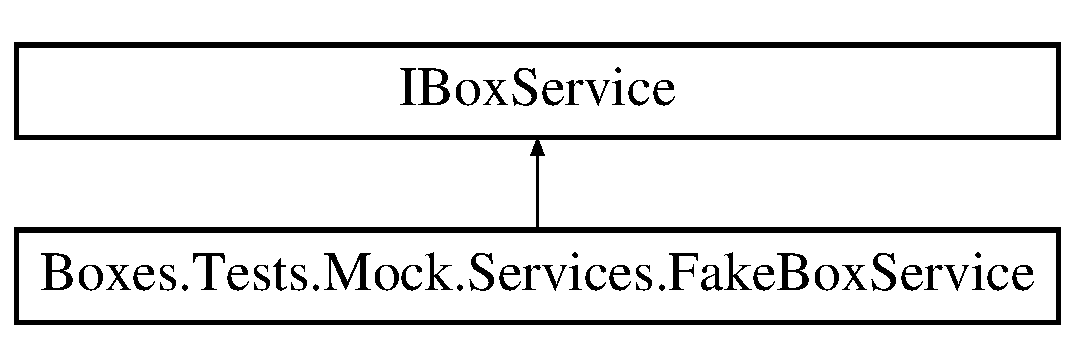
\includegraphics[height=2.000000cm]{class_boxes_1_1_tests_1_1_mock_1_1_services_1_1_fake_box_service}
\end{center}
\end{figure}
\subsection*{Fonctions membres publiques}
\begin{DoxyCompactItemize}
\item 
\hyperlink{class_boxes_1_1_tests_1_1_mock_1_1_services_1_1_fake_box_service_ae1e766e11e7021f30f6d65fe8be5c2d4}{Fake\+Box\+Service} ()
\begin{DoxyCompactList}\small\item\em Constructeur non paramétré qui initialise la liste des boites fictivement créées. \end{DoxyCompactList}\item 
Task \hyperlink{class_boxes_1_1_tests_1_1_mock_1_1_services_1_1_fake_box_service_abf7f2b2aa828502c97cdfe5e4ded4385}{Attach\+User\+Async} (Box box, User user)
\item 
Task$<$ Box $>$ \hyperlink{class_boxes_1_1_tests_1_1_mock_1_1_services_1_1_fake_box_service_a5c786507b63fd61dfdbaa2e78279884b}{Create\+Async} (Box box)
\item 
Task$<$ List$<$ Box $>$ $>$ \hyperlink{class_boxes_1_1_tests_1_1_mock_1_1_services_1_1_fake_box_service_a66667dfe33b89e4711ad39d1aa21f6d6}{Get\+By\+User\+Async} (User user)
\item 
Task$<$ List$<$ Box $>$ $>$ \hyperlink{class_boxes_1_1_tests_1_1_mock_1_1_services_1_1_fake_box_service_a32fa7ee58f8832c0d2a50aa3d5a16ae7}{Get\+Search\+Results\+Async} (string terms)
\item 
Task$<$ List$<$ Box $>$ $>$ \hyperlink{class_boxes_1_1_tests_1_1_mock_1_1_services_1_1_fake_box_service_a3e1e5288bf9e004117ae1e51fcff732f}{Get\+Top\+Async} ()
\item 
Task$<$ Box $>$ \hyperlink{class_boxes_1_1_tests_1_1_mock_1_1_services_1_1_fake_box_service_aef2d07809b5d9c4f1943ffba8d45c6c4}{Update\+Async} (Box box)
\item 
Task \hyperlink{class_boxes_1_1_tests_1_1_mock_1_1_services_1_1_fake_box_service_ae28d6ad5177e6ca1b6f8c0fbfc6e6370}{Delete\+Async} (Box box)
\item 
Task \hyperlink{class_boxes_1_1_tests_1_1_mock_1_1_services_1_1_fake_box_service_afc335b64bc641c738825851b605494a2}{Detach\+User\+Async} (Box box, User user)
\end{DoxyCompactItemize}
\subsection*{Propriétés}
\begin{DoxyCompactItemize}
\item 
List$<$ Box $>$ \hyperlink{class_boxes_1_1_tests_1_1_mock_1_1_services_1_1_fake_box_service_a3569dfb32a10167dcb57b87991f8e958}{Boxes}\hspace{0.3cm}{\ttfamily  \mbox{[}get, private set\mbox{]}}
\begin{DoxyCompactList}\small\item\em Liste des boites fictivement créées. \end{DoxyCompactList}\end{DoxyCompactItemize}


\subsection{Description détaillée}
Service d\textquotesingle{}accès aux données fictives de l\textquotesingle{}entité Box. 



\subsection{Documentation des constructeurs et destructeur}
\index{Boxes\+::\+Tests\+::\+Mock\+::\+Services\+::\+Fake\+Box\+Service@{Boxes\+::\+Tests\+::\+Mock\+::\+Services\+::\+Fake\+Box\+Service}!Fake\+Box\+Service@{Fake\+Box\+Service}}
\index{Fake\+Box\+Service@{Fake\+Box\+Service}!Boxes\+::\+Tests\+::\+Mock\+::\+Services\+::\+Fake\+Box\+Service@{Boxes\+::\+Tests\+::\+Mock\+::\+Services\+::\+Fake\+Box\+Service}}
\subsubsection[{\texorpdfstring{Fake\+Box\+Service()}{FakeBoxService()}}]{\setlength{\rightskip}{0pt plus 5cm}Boxes.\+Tests.\+Mock.\+Services.\+Fake\+Box\+Service.\+Fake\+Box\+Service (
\begin{DoxyParamCaption}
{}
\end{DoxyParamCaption}
)}\hypertarget{class_boxes_1_1_tests_1_1_mock_1_1_services_1_1_fake_box_service_ae1e766e11e7021f30f6d65fe8be5c2d4}{}\label{class_boxes_1_1_tests_1_1_mock_1_1_services_1_1_fake_box_service_ae1e766e11e7021f30f6d65fe8be5c2d4}


Constructeur non paramétré qui initialise la liste des boites fictivement créées. 



\subsection{Documentation des fonctions membres}
\index{Boxes\+::\+Tests\+::\+Mock\+::\+Services\+::\+Fake\+Box\+Service@{Boxes\+::\+Tests\+::\+Mock\+::\+Services\+::\+Fake\+Box\+Service}!Attach\+User\+Async@{Attach\+User\+Async}}
\index{Attach\+User\+Async@{Attach\+User\+Async}!Boxes\+::\+Tests\+::\+Mock\+::\+Services\+::\+Fake\+Box\+Service@{Boxes\+::\+Tests\+::\+Mock\+::\+Services\+::\+Fake\+Box\+Service}}
\subsubsection[{\texorpdfstring{Attach\+User\+Async(\+Box box, User user)}{AttachUserAsync(Box box, User user)}}]{\setlength{\rightskip}{0pt plus 5cm}Task Boxes.\+Tests.\+Mock.\+Services.\+Fake\+Box\+Service.\+Attach\+User\+Async (
\begin{DoxyParamCaption}
\item[{Box}]{box, }
\item[{User}]{user}
\end{DoxyParamCaption}
)}\hypertarget{class_boxes_1_1_tests_1_1_mock_1_1_services_1_1_fake_box_service_abf7f2b2aa828502c97cdfe5e4ded4385}{}\label{class_boxes_1_1_tests_1_1_mock_1_1_services_1_1_fake_box_service_abf7f2b2aa828502c97cdfe5e4ded4385}




\index{Boxes\+::\+Tests\+::\+Mock\+::\+Services\+::\+Fake\+Box\+Service@{Boxes\+::\+Tests\+::\+Mock\+::\+Services\+::\+Fake\+Box\+Service}!Create\+Async@{Create\+Async}}
\index{Create\+Async@{Create\+Async}!Boxes\+::\+Tests\+::\+Mock\+::\+Services\+::\+Fake\+Box\+Service@{Boxes\+::\+Tests\+::\+Mock\+::\+Services\+::\+Fake\+Box\+Service}}
\subsubsection[{\texorpdfstring{Create\+Async(\+Box box)}{CreateAsync(Box box)}}]{\setlength{\rightskip}{0pt plus 5cm}Task$<$Box$>$ Boxes.\+Tests.\+Mock.\+Services.\+Fake\+Box\+Service.\+Create\+Async (
\begin{DoxyParamCaption}
\item[{Box}]{box}
\end{DoxyParamCaption}
)}\hypertarget{class_boxes_1_1_tests_1_1_mock_1_1_services_1_1_fake_box_service_a5c786507b63fd61dfdbaa2e78279884b}{}\label{class_boxes_1_1_tests_1_1_mock_1_1_services_1_1_fake_box_service_a5c786507b63fd61dfdbaa2e78279884b}




\index{Boxes\+::\+Tests\+::\+Mock\+::\+Services\+::\+Fake\+Box\+Service@{Boxes\+::\+Tests\+::\+Mock\+::\+Services\+::\+Fake\+Box\+Service}!Delete\+Async@{Delete\+Async}}
\index{Delete\+Async@{Delete\+Async}!Boxes\+::\+Tests\+::\+Mock\+::\+Services\+::\+Fake\+Box\+Service@{Boxes\+::\+Tests\+::\+Mock\+::\+Services\+::\+Fake\+Box\+Service}}
\subsubsection[{\texorpdfstring{Delete\+Async(\+Box box)}{DeleteAsync(Box box)}}]{\setlength{\rightskip}{0pt plus 5cm}Task Boxes.\+Tests.\+Mock.\+Services.\+Fake\+Box\+Service.\+Delete\+Async (
\begin{DoxyParamCaption}
\item[{Box}]{box}
\end{DoxyParamCaption}
)}\hypertarget{class_boxes_1_1_tests_1_1_mock_1_1_services_1_1_fake_box_service_ae28d6ad5177e6ca1b6f8c0fbfc6e6370}{}\label{class_boxes_1_1_tests_1_1_mock_1_1_services_1_1_fake_box_service_ae28d6ad5177e6ca1b6f8c0fbfc6e6370}




\index{Boxes\+::\+Tests\+::\+Mock\+::\+Services\+::\+Fake\+Box\+Service@{Boxes\+::\+Tests\+::\+Mock\+::\+Services\+::\+Fake\+Box\+Service}!Detach\+User\+Async@{Detach\+User\+Async}}
\index{Detach\+User\+Async@{Detach\+User\+Async}!Boxes\+::\+Tests\+::\+Mock\+::\+Services\+::\+Fake\+Box\+Service@{Boxes\+::\+Tests\+::\+Mock\+::\+Services\+::\+Fake\+Box\+Service}}
\subsubsection[{\texorpdfstring{Detach\+User\+Async(\+Box box, User user)}{DetachUserAsync(Box box, User user)}}]{\setlength{\rightskip}{0pt plus 5cm}Task Boxes.\+Tests.\+Mock.\+Services.\+Fake\+Box\+Service.\+Detach\+User\+Async (
\begin{DoxyParamCaption}
\item[{Box}]{box, }
\item[{User}]{user}
\end{DoxyParamCaption}
)}\hypertarget{class_boxes_1_1_tests_1_1_mock_1_1_services_1_1_fake_box_service_afc335b64bc641c738825851b605494a2}{}\label{class_boxes_1_1_tests_1_1_mock_1_1_services_1_1_fake_box_service_afc335b64bc641c738825851b605494a2}




\index{Boxes\+::\+Tests\+::\+Mock\+::\+Services\+::\+Fake\+Box\+Service@{Boxes\+::\+Tests\+::\+Mock\+::\+Services\+::\+Fake\+Box\+Service}!Get\+By\+User\+Async@{Get\+By\+User\+Async}}
\index{Get\+By\+User\+Async@{Get\+By\+User\+Async}!Boxes\+::\+Tests\+::\+Mock\+::\+Services\+::\+Fake\+Box\+Service@{Boxes\+::\+Tests\+::\+Mock\+::\+Services\+::\+Fake\+Box\+Service}}
\subsubsection[{\texorpdfstring{Get\+By\+User\+Async(\+User user)}{GetByUserAsync(User user)}}]{\setlength{\rightskip}{0pt plus 5cm}Task$<$List$<$Box$>$ $>$ Boxes.\+Tests.\+Mock.\+Services.\+Fake\+Box\+Service.\+Get\+By\+User\+Async (
\begin{DoxyParamCaption}
\item[{User}]{user}
\end{DoxyParamCaption}
)}\hypertarget{class_boxes_1_1_tests_1_1_mock_1_1_services_1_1_fake_box_service_a66667dfe33b89e4711ad39d1aa21f6d6}{}\label{class_boxes_1_1_tests_1_1_mock_1_1_services_1_1_fake_box_service_a66667dfe33b89e4711ad39d1aa21f6d6}




\index{Boxes\+::\+Tests\+::\+Mock\+::\+Services\+::\+Fake\+Box\+Service@{Boxes\+::\+Tests\+::\+Mock\+::\+Services\+::\+Fake\+Box\+Service}!Get\+Search\+Results\+Async@{Get\+Search\+Results\+Async}}
\index{Get\+Search\+Results\+Async@{Get\+Search\+Results\+Async}!Boxes\+::\+Tests\+::\+Mock\+::\+Services\+::\+Fake\+Box\+Service@{Boxes\+::\+Tests\+::\+Mock\+::\+Services\+::\+Fake\+Box\+Service}}
\subsubsection[{\texorpdfstring{Get\+Search\+Results\+Async(string terms)}{GetSearchResultsAsync(string terms)}}]{\setlength{\rightskip}{0pt plus 5cm}Task$<$List$<$Box$>$ $>$ Boxes.\+Tests.\+Mock.\+Services.\+Fake\+Box\+Service.\+Get\+Search\+Results\+Async (
\begin{DoxyParamCaption}
\item[{string}]{terms}
\end{DoxyParamCaption}
)}\hypertarget{class_boxes_1_1_tests_1_1_mock_1_1_services_1_1_fake_box_service_a32fa7ee58f8832c0d2a50aa3d5a16ae7}{}\label{class_boxes_1_1_tests_1_1_mock_1_1_services_1_1_fake_box_service_a32fa7ee58f8832c0d2a50aa3d5a16ae7}




\index{Boxes\+::\+Tests\+::\+Mock\+::\+Services\+::\+Fake\+Box\+Service@{Boxes\+::\+Tests\+::\+Mock\+::\+Services\+::\+Fake\+Box\+Service}!Get\+Top\+Async@{Get\+Top\+Async}}
\index{Get\+Top\+Async@{Get\+Top\+Async}!Boxes\+::\+Tests\+::\+Mock\+::\+Services\+::\+Fake\+Box\+Service@{Boxes\+::\+Tests\+::\+Mock\+::\+Services\+::\+Fake\+Box\+Service}}
\subsubsection[{\texorpdfstring{Get\+Top\+Async()}{GetTopAsync()}}]{\setlength{\rightskip}{0pt plus 5cm}Task$<$List$<$Box$>$ $>$ Boxes.\+Tests.\+Mock.\+Services.\+Fake\+Box\+Service.\+Get\+Top\+Async (
\begin{DoxyParamCaption}
{}
\end{DoxyParamCaption}
)}\hypertarget{class_boxes_1_1_tests_1_1_mock_1_1_services_1_1_fake_box_service_a3e1e5288bf9e004117ae1e51fcff732f}{}\label{class_boxes_1_1_tests_1_1_mock_1_1_services_1_1_fake_box_service_a3e1e5288bf9e004117ae1e51fcff732f}




\index{Boxes\+::\+Tests\+::\+Mock\+::\+Services\+::\+Fake\+Box\+Service@{Boxes\+::\+Tests\+::\+Mock\+::\+Services\+::\+Fake\+Box\+Service}!Update\+Async@{Update\+Async}}
\index{Update\+Async@{Update\+Async}!Boxes\+::\+Tests\+::\+Mock\+::\+Services\+::\+Fake\+Box\+Service@{Boxes\+::\+Tests\+::\+Mock\+::\+Services\+::\+Fake\+Box\+Service}}
\subsubsection[{\texorpdfstring{Update\+Async(\+Box box)}{UpdateAsync(Box box)}}]{\setlength{\rightskip}{0pt plus 5cm}Task$<$Box$>$ Boxes.\+Tests.\+Mock.\+Services.\+Fake\+Box\+Service.\+Update\+Async (
\begin{DoxyParamCaption}
\item[{Box}]{box}
\end{DoxyParamCaption}
)}\hypertarget{class_boxes_1_1_tests_1_1_mock_1_1_services_1_1_fake_box_service_aef2d07809b5d9c4f1943ffba8d45c6c4}{}\label{class_boxes_1_1_tests_1_1_mock_1_1_services_1_1_fake_box_service_aef2d07809b5d9c4f1943ffba8d45c6c4}






\subsection{Documentation des propriétés}
\index{Boxes\+::\+Tests\+::\+Mock\+::\+Services\+::\+Fake\+Box\+Service@{Boxes\+::\+Tests\+::\+Mock\+::\+Services\+::\+Fake\+Box\+Service}!Boxes@{Boxes}}
\index{Boxes@{Boxes}!Boxes\+::\+Tests\+::\+Mock\+::\+Services\+::\+Fake\+Box\+Service@{Boxes\+::\+Tests\+::\+Mock\+::\+Services\+::\+Fake\+Box\+Service}}
\subsubsection[{\texorpdfstring{Boxes}{Boxes}}]{\setlength{\rightskip}{0pt plus 5cm}List$<$Box$>$ Boxes.\+Tests.\+Mock.\+Services.\+Fake\+Box\+Service.\+Boxes\hspace{0.3cm}{\ttfamily [get]}, {\ttfamily [private set]}}\hypertarget{class_boxes_1_1_tests_1_1_mock_1_1_services_1_1_fake_box_service_a3569dfb32a10167dcb57b87991f8e958}{}\label{class_boxes_1_1_tests_1_1_mock_1_1_services_1_1_fake_box_service_a3569dfb32a10167dcb57b87991f8e958}


Liste des boites fictivement créées. 



La documentation de cette classe a été générée à partir du fichier suivant \+:\begin{DoxyCompactItemize}
\item 
C\+:/\+Users/thoma/\+One\+Drive/\+Documents/\+Visual Studio 2015/\+Projects/\+Boxes/\+Boxes.\+Tests/\+Mock/\+Services/\hyperlink{_fake_box_service_8cs}{Fake\+Box\+Service.\+cs}\end{DoxyCompactItemize}

\hypertarget{class_boxes_1_1_tests_1_1_mock_1_1_services_1_1_fake_comment_service}{}\section{Référence de la classe Boxes.\+Tests.\+Mock.\+Services.\+Fake\+Comment\+Service}
\label{class_boxes_1_1_tests_1_1_mock_1_1_services_1_1_fake_comment_service}\index{Boxes.\+Tests.\+Mock.\+Services.\+Fake\+Comment\+Service@{Boxes.\+Tests.\+Mock.\+Services.\+Fake\+Comment\+Service}}


Service d\textquotesingle{}accès aux données fictives de l\textquotesingle{}entité Post.  


Graphe d\textquotesingle{}héritage de Boxes.\+Tests.\+Mock.\+Services.\+Fake\+Comment\+Service\+:\begin{figure}[H]
\begin{center}
\leavevmode
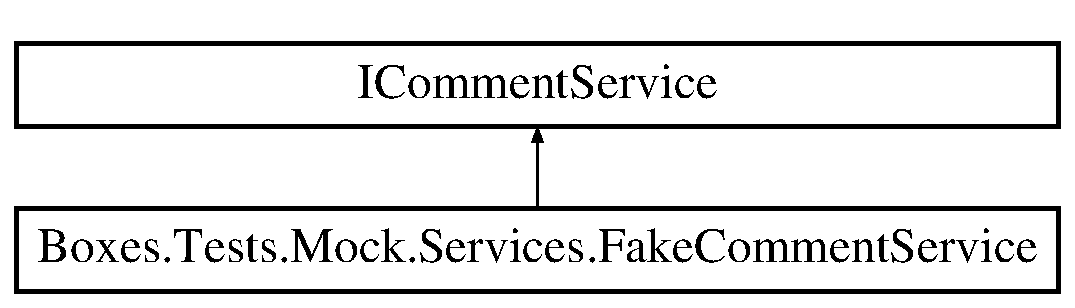
\includegraphics[height=2.000000cm]{class_boxes_1_1_tests_1_1_mock_1_1_services_1_1_fake_comment_service}
\end{center}
\end{figure}
\subsection*{Fonctions membres publiques}
\begin{DoxyCompactItemize}
\item 
\hyperlink{class_boxes_1_1_tests_1_1_mock_1_1_services_1_1_fake_comment_service_a5d6567f4d50c7bb1469b0e81f582e428}{Fake\+Comment\+Service} ()
\begin{DoxyCompactList}\small\item\em Constructeur non paramétré qui initialise la liste des commentaires fictifs. \end{DoxyCompactList}\item 
Task$<$ Comment $>$ \hyperlink{class_boxes_1_1_tests_1_1_mock_1_1_services_1_1_fake_comment_service_a5ecc4acf78554c99498bef433dadd1a7}{Create\+Async} (Comment comment)
\item 
Task$<$ List$<$ Comment $>$ $>$ \hyperlink{class_boxes_1_1_tests_1_1_mock_1_1_services_1_1_fake_comment_service_a79ddddd76c921a8351c6b97fc71cb238}{Get\+By\+Post\+Async} (Post post)
\end{DoxyCompactItemize}
\subsection*{Propriétés}
\begin{DoxyCompactItemize}
\item 
List$<$ Comment $>$ \hyperlink{class_boxes_1_1_tests_1_1_mock_1_1_services_1_1_fake_comment_service_aad282113b2428dc23320b01ab86ab427}{Comments}\hspace{0.3cm}{\ttfamily  \mbox{[}get, private set\mbox{]}}
\begin{DoxyCompactList}\small\item\em Liste de commentaires fictifs. \end{DoxyCompactList}\end{DoxyCompactItemize}


\subsection{Description détaillée}
Service d\textquotesingle{}accès aux données fictives de l\textquotesingle{}entité Post. 



\subsection{Documentation des constructeurs et destructeur}
\index{Boxes\+::\+Tests\+::\+Mock\+::\+Services\+::\+Fake\+Comment\+Service@{Boxes\+::\+Tests\+::\+Mock\+::\+Services\+::\+Fake\+Comment\+Service}!Fake\+Comment\+Service@{Fake\+Comment\+Service}}
\index{Fake\+Comment\+Service@{Fake\+Comment\+Service}!Boxes\+::\+Tests\+::\+Mock\+::\+Services\+::\+Fake\+Comment\+Service@{Boxes\+::\+Tests\+::\+Mock\+::\+Services\+::\+Fake\+Comment\+Service}}
\subsubsection[{\texorpdfstring{Fake\+Comment\+Service()}{FakeCommentService()}}]{\setlength{\rightskip}{0pt plus 5cm}Boxes.\+Tests.\+Mock.\+Services.\+Fake\+Comment\+Service.\+Fake\+Comment\+Service (
\begin{DoxyParamCaption}
{}
\end{DoxyParamCaption}
)}\hypertarget{class_boxes_1_1_tests_1_1_mock_1_1_services_1_1_fake_comment_service_a5d6567f4d50c7bb1469b0e81f582e428}{}\label{class_boxes_1_1_tests_1_1_mock_1_1_services_1_1_fake_comment_service_a5d6567f4d50c7bb1469b0e81f582e428}


Constructeur non paramétré qui initialise la liste des commentaires fictifs. 



\subsection{Documentation des fonctions membres}
\index{Boxes\+::\+Tests\+::\+Mock\+::\+Services\+::\+Fake\+Comment\+Service@{Boxes\+::\+Tests\+::\+Mock\+::\+Services\+::\+Fake\+Comment\+Service}!Create\+Async@{Create\+Async}}
\index{Create\+Async@{Create\+Async}!Boxes\+::\+Tests\+::\+Mock\+::\+Services\+::\+Fake\+Comment\+Service@{Boxes\+::\+Tests\+::\+Mock\+::\+Services\+::\+Fake\+Comment\+Service}}
\subsubsection[{\texorpdfstring{Create\+Async(\+Comment comment)}{CreateAsync(Comment comment)}}]{\setlength{\rightskip}{0pt plus 5cm}Task$<$Comment$>$ Boxes.\+Tests.\+Mock.\+Services.\+Fake\+Comment\+Service.\+Create\+Async (
\begin{DoxyParamCaption}
\item[{Comment}]{comment}
\end{DoxyParamCaption}
)}\hypertarget{class_boxes_1_1_tests_1_1_mock_1_1_services_1_1_fake_comment_service_a5ecc4acf78554c99498bef433dadd1a7}{}\label{class_boxes_1_1_tests_1_1_mock_1_1_services_1_1_fake_comment_service_a5ecc4acf78554c99498bef433dadd1a7}




\index{Boxes\+::\+Tests\+::\+Mock\+::\+Services\+::\+Fake\+Comment\+Service@{Boxes\+::\+Tests\+::\+Mock\+::\+Services\+::\+Fake\+Comment\+Service}!Get\+By\+Post\+Async@{Get\+By\+Post\+Async}}
\index{Get\+By\+Post\+Async@{Get\+By\+Post\+Async}!Boxes\+::\+Tests\+::\+Mock\+::\+Services\+::\+Fake\+Comment\+Service@{Boxes\+::\+Tests\+::\+Mock\+::\+Services\+::\+Fake\+Comment\+Service}}
\subsubsection[{\texorpdfstring{Get\+By\+Post\+Async(\+Post post)}{GetByPostAsync(Post post)}}]{\setlength{\rightskip}{0pt plus 5cm}Task$<$List$<$Comment$>$ $>$ Boxes.\+Tests.\+Mock.\+Services.\+Fake\+Comment\+Service.\+Get\+By\+Post\+Async (
\begin{DoxyParamCaption}
\item[{Post}]{post}
\end{DoxyParamCaption}
)}\hypertarget{class_boxes_1_1_tests_1_1_mock_1_1_services_1_1_fake_comment_service_a79ddddd76c921a8351c6b97fc71cb238}{}\label{class_boxes_1_1_tests_1_1_mock_1_1_services_1_1_fake_comment_service_a79ddddd76c921a8351c6b97fc71cb238}






\subsection{Documentation des propriétés}
\index{Boxes\+::\+Tests\+::\+Mock\+::\+Services\+::\+Fake\+Comment\+Service@{Boxes\+::\+Tests\+::\+Mock\+::\+Services\+::\+Fake\+Comment\+Service}!Comments@{Comments}}
\index{Comments@{Comments}!Boxes\+::\+Tests\+::\+Mock\+::\+Services\+::\+Fake\+Comment\+Service@{Boxes\+::\+Tests\+::\+Mock\+::\+Services\+::\+Fake\+Comment\+Service}}
\subsubsection[{\texorpdfstring{Comments}{Comments}}]{\setlength{\rightskip}{0pt plus 5cm}List$<$Comment$>$ Boxes.\+Tests.\+Mock.\+Services.\+Fake\+Comment\+Service.\+Comments\hspace{0.3cm}{\ttfamily [get]}, {\ttfamily [private set]}}\hypertarget{class_boxes_1_1_tests_1_1_mock_1_1_services_1_1_fake_comment_service_aad282113b2428dc23320b01ab86ab427}{}\label{class_boxes_1_1_tests_1_1_mock_1_1_services_1_1_fake_comment_service_aad282113b2428dc23320b01ab86ab427}


Liste de commentaires fictifs. 



La documentation de cette classe a été générée à partir du fichier suivant \+:\begin{DoxyCompactItemize}
\item 
C\+:/\+Users/thoma/\+One\+Drive/\+Documents/\+Visual Studio 2015/\+Projects/\+Boxes/\+Boxes.\+Tests/\+Mock/\+Services/\hyperlink{_fake_comment_service_8cs}{Fake\+Comment\+Service.\+cs}\end{DoxyCompactItemize}

\hypertarget{class_boxes_1_1_tests_1_1_mock_1_1_services_1_1_fake_localization_service}{}\section{Référence de la classe Boxes.\+Tests.\+Mock.\+Services.\+Fake\+Localization\+Service}
\label{class_boxes_1_1_tests_1_1_mock_1_1_services_1_1_fake_localization_service}\index{Boxes.\+Tests.\+Mock.\+Services.\+Fake\+Localization\+Service@{Boxes.\+Tests.\+Mock.\+Services.\+Fake\+Localization\+Service}}


Service d\textquotesingle{}accès aux données fictives de localization.  


Graphe d\textquotesingle{}héritage de Boxes.\+Tests.\+Mock.\+Services.\+Fake\+Localization\+Service\+:\begin{figure}[H]
\begin{center}
\leavevmode
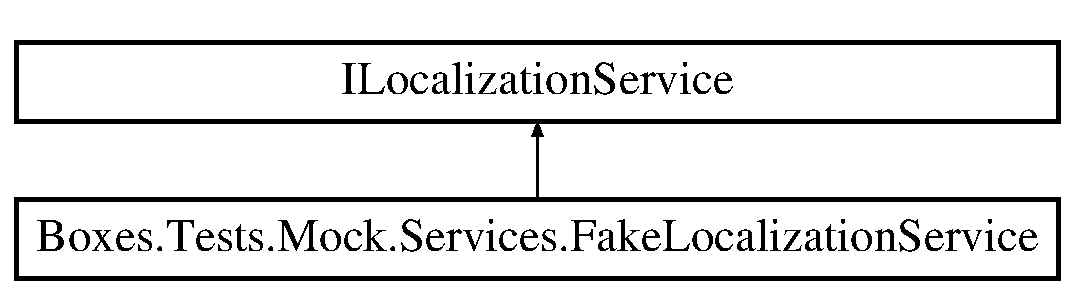
\includegraphics[height=2.000000cm]{class_boxes_1_1_tests_1_1_mock_1_1_services_1_1_fake_localization_service}
\end{center}
\end{figure}
\subsection*{Fonctions membres publiques}
\begin{DoxyCompactItemize}
\item 
\hyperlink{class_boxes_1_1_tests_1_1_mock_1_1_services_1_1_fake_localization_service_ae9f699f8c57a498f3e2cec76f118e57b}{Fake\+Localization\+Service} ()
\begin{DoxyCompactList}\small\item\em Constructeur non paramétré qui initialise les resources fictives de localization. \end{DoxyCompactList}\item 
string \hyperlink{class_boxes_1_1_tests_1_1_mock_1_1_services_1_1_fake_localization_service_ae8683fc6f58a0f8b223144f055d26a31}{Get\+String} (string resource\+Key)
\end{DoxyCompactItemize}
\subsection*{Attributs privés}
\begin{DoxyCompactItemize}
\item 
Dictionary$<$ string, string $>$ \hyperlink{class_boxes_1_1_tests_1_1_mock_1_1_services_1_1_fake_localization_service_a330124480defe0c22cb0b12037c44450}{resources}
\begin{DoxyCompactList}\small\item\em Stock les resources fictives de localization. \end{DoxyCompactList}\end{DoxyCompactItemize}


\subsection{Description détaillée}
Service d\textquotesingle{}accès aux données fictives de localization. 



\subsection{Documentation des constructeurs et destructeur}
\index{Boxes\+::\+Tests\+::\+Mock\+::\+Services\+::\+Fake\+Localization\+Service@{Boxes\+::\+Tests\+::\+Mock\+::\+Services\+::\+Fake\+Localization\+Service}!Fake\+Localization\+Service@{Fake\+Localization\+Service}}
\index{Fake\+Localization\+Service@{Fake\+Localization\+Service}!Boxes\+::\+Tests\+::\+Mock\+::\+Services\+::\+Fake\+Localization\+Service@{Boxes\+::\+Tests\+::\+Mock\+::\+Services\+::\+Fake\+Localization\+Service}}
\subsubsection[{\texorpdfstring{Fake\+Localization\+Service()}{FakeLocalizationService()}}]{\setlength{\rightskip}{0pt plus 5cm}Boxes.\+Tests.\+Mock.\+Services.\+Fake\+Localization\+Service.\+Fake\+Localization\+Service (
\begin{DoxyParamCaption}
{}
\end{DoxyParamCaption}
)}\hypertarget{class_boxes_1_1_tests_1_1_mock_1_1_services_1_1_fake_localization_service_ae9f699f8c57a498f3e2cec76f118e57b}{}\label{class_boxes_1_1_tests_1_1_mock_1_1_services_1_1_fake_localization_service_ae9f699f8c57a498f3e2cec76f118e57b}


Constructeur non paramétré qui initialise les resources fictives de localization. 



\subsection{Documentation des fonctions membres}
\index{Boxes\+::\+Tests\+::\+Mock\+::\+Services\+::\+Fake\+Localization\+Service@{Boxes\+::\+Tests\+::\+Mock\+::\+Services\+::\+Fake\+Localization\+Service}!Get\+String@{Get\+String}}
\index{Get\+String@{Get\+String}!Boxes\+::\+Tests\+::\+Mock\+::\+Services\+::\+Fake\+Localization\+Service@{Boxes\+::\+Tests\+::\+Mock\+::\+Services\+::\+Fake\+Localization\+Service}}
\subsubsection[{\texorpdfstring{Get\+String(string resource\+Key)}{GetString(string resourceKey)}}]{\setlength{\rightskip}{0pt plus 5cm}string Boxes.\+Tests.\+Mock.\+Services.\+Fake\+Localization\+Service.\+Get\+String (
\begin{DoxyParamCaption}
\item[{string}]{resource\+Key}
\end{DoxyParamCaption}
)}\hypertarget{class_boxes_1_1_tests_1_1_mock_1_1_services_1_1_fake_localization_service_ae8683fc6f58a0f8b223144f055d26a31}{}\label{class_boxes_1_1_tests_1_1_mock_1_1_services_1_1_fake_localization_service_ae8683fc6f58a0f8b223144f055d26a31}






\subsection{Documentation des données membres}
\index{Boxes\+::\+Tests\+::\+Mock\+::\+Services\+::\+Fake\+Localization\+Service@{Boxes\+::\+Tests\+::\+Mock\+::\+Services\+::\+Fake\+Localization\+Service}!resources@{resources}}
\index{resources@{resources}!Boxes\+::\+Tests\+::\+Mock\+::\+Services\+::\+Fake\+Localization\+Service@{Boxes\+::\+Tests\+::\+Mock\+::\+Services\+::\+Fake\+Localization\+Service}}
\subsubsection[{\texorpdfstring{resources}{resources}}]{\setlength{\rightskip}{0pt plus 5cm}Dictionary$<$string, string$>$ Boxes.\+Tests.\+Mock.\+Services.\+Fake\+Localization\+Service.\+resources\hspace{0.3cm}{\ttfamily [private]}}\hypertarget{class_boxes_1_1_tests_1_1_mock_1_1_services_1_1_fake_localization_service_a330124480defe0c22cb0b12037c44450}{}\label{class_boxes_1_1_tests_1_1_mock_1_1_services_1_1_fake_localization_service_a330124480defe0c22cb0b12037c44450}


Stock les resources fictives de localization. 



La documentation de cette classe a été générée à partir du fichier suivant \+:\begin{DoxyCompactItemize}
\item 
C\+:/\+Users/thoma/\+One\+Drive/\+Documents/\+Visual Studio 2015/\+Projects/\+Boxes/\+Boxes.\+Tests/\+Mock/\+Services/\hyperlink{_fake_localization_service_8cs}{Fake\+Localization\+Service.\+cs}\end{DoxyCompactItemize}

\hypertarget{class_boxes_1_1_tests_1_1_mock_1_1_services_1_1_fake_navigation_service}{}\section{Référence de la classe Boxes.\+Tests.\+Mock.\+Services.\+Fake\+Navigation\+Service}
\label{class_boxes_1_1_tests_1_1_mock_1_1_services_1_1_fake_navigation_service}\index{Boxes.\+Tests.\+Mock.\+Services.\+Fake\+Navigation\+Service@{Boxes.\+Tests.\+Mock.\+Services.\+Fake\+Navigation\+Service}}


Service de navigation fictif dont on peut récupérer la page actuellement affichée avec la propriété {\ttfamily Current\+Page\+Key}. Le stack de navigation est enregistré dans une liste (champ {\ttfamily navigation\+Stack}).  


Graphe d\textquotesingle{}héritage de Boxes.\+Tests.\+Mock.\+Services.\+Fake\+Navigation\+Service\+:\begin{figure}[H]
\begin{center}
\leavevmode
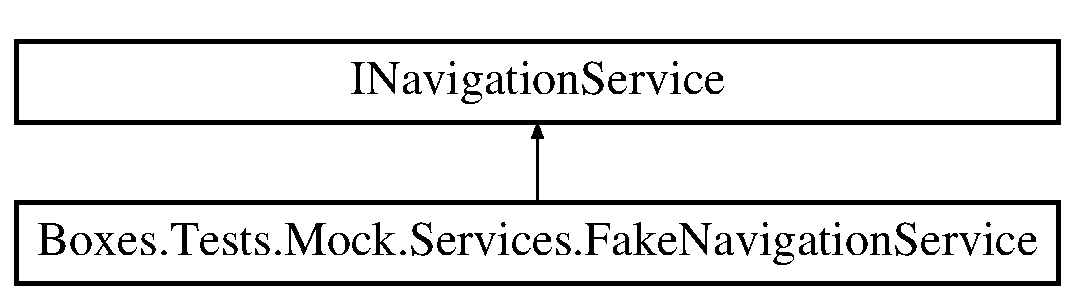
\includegraphics[height=2.000000cm]{class_boxes_1_1_tests_1_1_mock_1_1_services_1_1_fake_navigation_service}
\end{center}
\end{figure}
\subsection*{Fonctions membres publiques}
\begin{DoxyCompactItemize}
\item 
\hyperlink{class_boxes_1_1_tests_1_1_mock_1_1_services_1_1_fake_navigation_service_aceadde6c61562278fce55e793434f934}{Fake\+Navigation\+Service} ()
\begin{DoxyCompactList}\small\item\em Constructeur non paramétré qui initialise le stack de navigation. \end{DoxyCompactList}\item 
void \hyperlink{class_boxes_1_1_tests_1_1_mock_1_1_services_1_1_fake_navigation_service_a27266175146d23c89c997e637e3c8813}{Go\+Back} ()
\begin{DoxyCompactList}\small\item\em Navigue vers la page précédente dans le stack de navigation. \end{DoxyCompactList}\item 
void \hyperlink{class_boxes_1_1_tests_1_1_mock_1_1_services_1_1_fake_navigation_service_a0459ed72ee0a07da55556de2cff5182f}{Navigate\+To} (string page\+Key)
\begin{DoxyCompactList}\small\item\em Navigue vers la page de clé {\itshape page\+Key} . La propriété {\ttfamily Current\+Page\+Key} prend donc la valeur de {\itshape page\+Key} . \end{DoxyCompactList}\item 
void \hyperlink{class_boxes_1_1_tests_1_1_mock_1_1_services_1_1_fake_navigation_service_a4471c5eaa01e36727efd13c6b25936d8}{Navigate\+To} (string page\+Key, object parameter)
\begin{DoxyCompactList}\small\item\em Navigue vers la page de clé {\itshape page\+Key}  en lui passant un paramètre. La propriété {\ttfamily Current\+Page\+Key} prend donc la valeur de {\itshape page\+Key} . La propriété {\ttfamily Current\+Page\+Parameter} prend la valeur de {\itshape parameter} . \end{DoxyCompactList}\end{DoxyCompactItemize}
\subsection*{Propriétés}
\begin{DoxyCompactItemize}
\item 
string \hyperlink{class_boxes_1_1_tests_1_1_mock_1_1_services_1_1_fake_navigation_service_ac56e00a3392fc0d8370e34f2b3665021}{Current\+Page\+Key}\hspace{0.3cm}{\ttfamily  \mbox{[}get, private set\mbox{]}}
\begin{DoxyCompactList}\small\item\em Clé de la page actuellement affichée. \end{DoxyCompactList}\item 
object \hyperlink{class_boxes_1_1_tests_1_1_mock_1_1_services_1_1_fake_navigation_service_a6a5a1f38263717cf9dbfada81deb79d3}{Current\+Page\+Parameter}\hspace{0.3cm}{\ttfamily  \mbox{[}get\mbox{]}}
\begin{DoxyCompactList}\small\item\em Paramètre transmis à la page actuellement affichée. \end{DoxyCompactList}\end{DoxyCompactItemize}
\subsection*{Attributs privés}
\begin{DoxyCompactItemize}
\item 
Dictionary$<$ string, object $>$ \hyperlink{class_boxes_1_1_tests_1_1_mock_1_1_services_1_1_fake_navigation_service_ad295920ed186a7b945b3597c635f12e0}{navigation\+Stack}
\begin{DoxyCompactList}\small\item\em Stack de navigation. \end{DoxyCompactList}\end{DoxyCompactItemize}


\subsection{Description détaillée}
Service de navigation fictif dont on peut récupérer la page actuellement affichée avec la propriété {\ttfamily Current\+Page\+Key}. Le stack de navigation est enregistré dans une liste (champ {\ttfamily navigation\+Stack}). 



\subsection{Documentation des constructeurs et destructeur}
\index{Boxes\+::\+Tests\+::\+Mock\+::\+Services\+::\+Fake\+Navigation\+Service@{Boxes\+::\+Tests\+::\+Mock\+::\+Services\+::\+Fake\+Navigation\+Service}!Fake\+Navigation\+Service@{Fake\+Navigation\+Service}}
\index{Fake\+Navigation\+Service@{Fake\+Navigation\+Service}!Boxes\+::\+Tests\+::\+Mock\+::\+Services\+::\+Fake\+Navigation\+Service@{Boxes\+::\+Tests\+::\+Mock\+::\+Services\+::\+Fake\+Navigation\+Service}}
\subsubsection[{\texorpdfstring{Fake\+Navigation\+Service()}{FakeNavigationService()}}]{\setlength{\rightskip}{0pt plus 5cm}Boxes.\+Tests.\+Mock.\+Services.\+Fake\+Navigation\+Service.\+Fake\+Navigation\+Service (
\begin{DoxyParamCaption}
{}
\end{DoxyParamCaption}
)}\hypertarget{class_boxes_1_1_tests_1_1_mock_1_1_services_1_1_fake_navigation_service_aceadde6c61562278fce55e793434f934}{}\label{class_boxes_1_1_tests_1_1_mock_1_1_services_1_1_fake_navigation_service_aceadde6c61562278fce55e793434f934}


Constructeur non paramétré qui initialise le stack de navigation. 



\subsection{Documentation des fonctions membres}
\index{Boxes\+::\+Tests\+::\+Mock\+::\+Services\+::\+Fake\+Navigation\+Service@{Boxes\+::\+Tests\+::\+Mock\+::\+Services\+::\+Fake\+Navigation\+Service}!Go\+Back@{Go\+Back}}
\index{Go\+Back@{Go\+Back}!Boxes\+::\+Tests\+::\+Mock\+::\+Services\+::\+Fake\+Navigation\+Service@{Boxes\+::\+Tests\+::\+Mock\+::\+Services\+::\+Fake\+Navigation\+Service}}
\subsubsection[{\texorpdfstring{Go\+Back()}{GoBack()}}]{\setlength{\rightskip}{0pt plus 5cm}void Boxes.\+Tests.\+Mock.\+Services.\+Fake\+Navigation\+Service.\+Go\+Back (
\begin{DoxyParamCaption}
{}
\end{DoxyParamCaption}
)}\hypertarget{class_boxes_1_1_tests_1_1_mock_1_1_services_1_1_fake_navigation_service_a27266175146d23c89c997e637e3c8813}{}\label{class_boxes_1_1_tests_1_1_mock_1_1_services_1_1_fake_navigation_service_a27266175146d23c89c997e637e3c8813}


Navigue vers la page précédente dans le stack de navigation. 

\index{Boxes\+::\+Tests\+::\+Mock\+::\+Services\+::\+Fake\+Navigation\+Service@{Boxes\+::\+Tests\+::\+Mock\+::\+Services\+::\+Fake\+Navigation\+Service}!Navigate\+To@{Navigate\+To}}
\index{Navigate\+To@{Navigate\+To}!Boxes\+::\+Tests\+::\+Mock\+::\+Services\+::\+Fake\+Navigation\+Service@{Boxes\+::\+Tests\+::\+Mock\+::\+Services\+::\+Fake\+Navigation\+Service}}
\subsubsection[{\texorpdfstring{Navigate\+To(string page\+Key)}{NavigateTo(string pageKey)}}]{\setlength{\rightskip}{0pt plus 5cm}void Boxes.\+Tests.\+Mock.\+Services.\+Fake\+Navigation\+Service.\+Navigate\+To (
\begin{DoxyParamCaption}
\item[{string}]{page\+Key}
\end{DoxyParamCaption}
)}\hypertarget{class_boxes_1_1_tests_1_1_mock_1_1_services_1_1_fake_navigation_service_a0459ed72ee0a07da55556de2cff5182f}{}\label{class_boxes_1_1_tests_1_1_mock_1_1_services_1_1_fake_navigation_service_a0459ed72ee0a07da55556de2cff5182f}


Navigue vers la page de clé {\itshape page\+Key} . La propriété {\ttfamily Current\+Page\+Key} prend donc la valeur de {\itshape page\+Key} . 


\begin{DoxyParams}{Paramètres}
{\em page\+Key} & Clé de la page sur laquelle naviguer. \\
\hline
\end{DoxyParams}
\index{Boxes\+::\+Tests\+::\+Mock\+::\+Services\+::\+Fake\+Navigation\+Service@{Boxes\+::\+Tests\+::\+Mock\+::\+Services\+::\+Fake\+Navigation\+Service}!Navigate\+To@{Navigate\+To}}
\index{Navigate\+To@{Navigate\+To}!Boxes\+::\+Tests\+::\+Mock\+::\+Services\+::\+Fake\+Navigation\+Service@{Boxes\+::\+Tests\+::\+Mock\+::\+Services\+::\+Fake\+Navigation\+Service}}
\subsubsection[{\texorpdfstring{Navigate\+To(string page\+Key, object parameter)}{NavigateTo(string pageKey, object parameter)}}]{\setlength{\rightskip}{0pt plus 5cm}void Boxes.\+Tests.\+Mock.\+Services.\+Fake\+Navigation\+Service.\+Navigate\+To (
\begin{DoxyParamCaption}
\item[{string}]{page\+Key, }
\item[{object}]{parameter}
\end{DoxyParamCaption}
)}\hypertarget{class_boxes_1_1_tests_1_1_mock_1_1_services_1_1_fake_navigation_service_a4471c5eaa01e36727efd13c6b25936d8}{}\label{class_boxes_1_1_tests_1_1_mock_1_1_services_1_1_fake_navigation_service_a4471c5eaa01e36727efd13c6b25936d8}


Navigue vers la page de clé {\itshape page\+Key}  en lui passant un paramètre. La propriété {\ttfamily Current\+Page\+Key} prend donc la valeur de {\itshape page\+Key} . La propriété {\ttfamily Current\+Page\+Parameter} prend la valeur de {\itshape parameter} . 


\begin{DoxyParams}{Paramètres}
{\em page\+Key} & Clé de la page sur laquelle naviguer. \\
\hline
{\em parameter} & Paramètre à passer à la page. \\
\hline
\end{DoxyParams}


\subsection{Documentation des données membres}
\index{Boxes\+::\+Tests\+::\+Mock\+::\+Services\+::\+Fake\+Navigation\+Service@{Boxes\+::\+Tests\+::\+Mock\+::\+Services\+::\+Fake\+Navigation\+Service}!navigation\+Stack@{navigation\+Stack}}
\index{navigation\+Stack@{navigation\+Stack}!Boxes\+::\+Tests\+::\+Mock\+::\+Services\+::\+Fake\+Navigation\+Service@{Boxes\+::\+Tests\+::\+Mock\+::\+Services\+::\+Fake\+Navigation\+Service}}
\subsubsection[{\texorpdfstring{navigation\+Stack}{navigationStack}}]{\setlength{\rightskip}{0pt plus 5cm}Dictionary$<$string, object$>$ Boxes.\+Tests.\+Mock.\+Services.\+Fake\+Navigation\+Service.\+navigation\+Stack\hspace{0.3cm}{\ttfamily [private]}}\hypertarget{class_boxes_1_1_tests_1_1_mock_1_1_services_1_1_fake_navigation_service_ad295920ed186a7b945b3597c635f12e0}{}\label{class_boxes_1_1_tests_1_1_mock_1_1_services_1_1_fake_navigation_service_ad295920ed186a7b945b3597c635f12e0}


Stack de navigation. 

A chaque fois qu\textquotesingle{}une navigation s\textquotesingle{}opère la page affichée s\textquotesingle{}inscrit dans ce dictionnaire (en clé). Le paramètre transmis à la page s\textquotesingle{}inscrit en valeur. 

\subsection{Documentation des propriétés}
\index{Boxes\+::\+Tests\+::\+Mock\+::\+Services\+::\+Fake\+Navigation\+Service@{Boxes\+::\+Tests\+::\+Mock\+::\+Services\+::\+Fake\+Navigation\+Service}!Current\+Page\+Key@{Current\+Page\+Key}}
\index{Current\+Page\+Key@{Current\+Page\+Key}!Boxes\+::\+Tests\+::\+Mock\+::\+Services\+::\+Fake\+Navigation\+Service@{Boxes\+::\+Tests\+::\+Mock\+::\+Services\+::\+Fake\+Navigation\+Service}}
\subsubsection[{\texorpdfstring{Current\+Page\+Key}{CurrentPageKey}}]{\setlength{\rightskip}{0pt plus 5cm}string Boxes.\+Tests.\+Mock.\+Services.\+Fake\+Navigation\+Service.\+Current\+Page\+Key\hspace{0.3cm}{\ttfamily [get]}, {\ttfamily [private set]}}\hypertarget{class_boxes_1_1_tests_1_1_mock_1_1_services_1_1_fake_navigation_service_ac56e00a3392fc0d8370e34f2b3665021}{}\label{class_boxes_1_1_tests_1_1_mock_1_1_services_1_1_fake_navigation_service_ac56e00a3392fc0d8370e34f2b3665021}


Clé de la page actuellement affichée. 

\index{Boxes\+::\+Tests\+::\+Mock\+::\+Services\+::\+Fake\+Navigation\+Service@{Boxes\+::\+Tests\+::\+Mock\+::\+Services\+::\+Fake\+Navigation\+Service}!Current\+Page\+Parameter@{Current\+Page\+Parameter}}
\index{Current\+Page\+Parameter@{Current\+Page\+Parameter}!Boxes\+::\+Tests\+::\+Mock\+::\+Services\+::\+Fake\+Navigation\+Service@{Boxes\+::\+Tests\+::\+Mock\+::\+Services\+::\+Fake\+Navigation\+Service}}
\subsubsection[{\texorpdfstring{Current\+Page\+Parameter}{CurrentPageParameter}}]{\setlength{\rightskip}{0pt plus 5cm}object Boxes.\+Tests.\+Mock.\+Services.\+Fake\+Navigation\+Service.\+Current\+Page\+Parameter\hspace{0.3cm}{\ttfamily [get]}}\hypertarget{class_boxes_1_1_tests_1_1_mock_1_1_services_1_1_fake_navigation_service_a6a5a1f38263717cf9dbfada81deb79d3}{}\label{class_boxes_1_1_tests_1_1_mock_1_1_services_1_1_fake_navigation_service_a6a5a1f38263717cf9dbfada81deb79d3}


Paramètre transmis à la page actuellement affichée. 



La documentation de cette classe a été générée à partir du fichier suivant \+:\begin{DoxyCompactItemize}
\item 
C\+:/\+Users/thoma/\+One\+Drive/\+Documents/\+Visual Studio 2015/\+Projects/\+Boxes/\+Boxes.\+Tests/\+Mock/\+Services/\hyperlink{_fake_navigation_service_8cs}{Fake\+Navigation\+Service.\+cs}\end{DoxyCompactItemize}

\hypertarget{class_boxes_1_1_tests_1_1_mock_1_1_services_1_1_fake_post_service}{}\section{Référence de la classe Boxes.\+Tests.\+Mock.\+Services.\+Fake\+Post\+Service}
\label{class_boxes_1_1_tests_1_1_mock_1_1_services_1_1_fake_post_service}\index{Boxes.\+Tests.\+Mock.\+Services.\+Fake\+Post\+Service@{Boxes.\+Tests.\+Mock.\+Services.\+Fake\+Post\+Service}}


Service d\textquotesingle{}accès aux données fictives de l\textquotesingle{}entité Post.  


Graphe d\textquotesingle{}héritage de Boxes.\+Tests.\+Mock.\+Services.\+Fake\+Post\+Service\+:\begin{figure}[H]
\begin{center}
\leavevmode
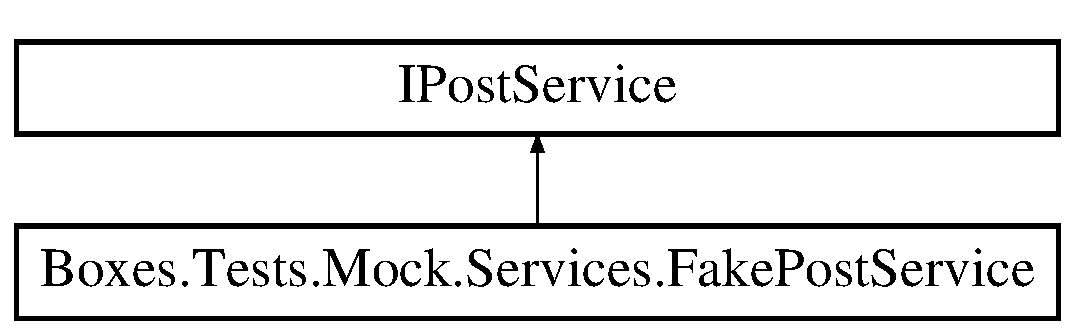
\includegraphics[height=2.000000cm]{class_boxes_1_1_tests_1_1_mock_1_1_services_1_1_fake_post_service}
\end{center}
\end{figure}
\subsection*{Fonctions membres publiques}
\begin{DoxyCompactItemize}
\item 
\hyperlink{class_boxes_1_1_tests_1_1_mock_1_1_services_1_1_fake_post_service_af5ed93d1526994a72e03389c2d33da67}{Fake\+Post\+Service} ()
\begin{DoxyCompactList}\small\item\em Constructeur non paramétré qui initialise la liste des posts fictivements créés. \end{DoxyCompactList}\item 
Task$<$ Post $>$ \hyperlink{class_boxes_1_1_tests_1_1_mock_1_1_services_1_1_fake_post_service_a353b1b5fe4a1fd04f2a7e40cec1a1810}{Create\+Async} (Post post)
\item 
Task$<$ List$<$ Post $>$ $>$ \hyperlink{class_boxes_1_1_tests_1_1_mock_1_1_services_1_1_fake_post_service_a42ecce94c2243bfa6d8833bd8db8344e}{Get\+By\+Box\+Async} (Box box)
\item 
Task$<$ List$<$ Post $>$ $>$ \hyperlink{class_boxes_1_1_tests_1_1_mock_1_1_services_1_1_fake_post_service_ad559e120252973aa279b7dfdc2043f9c}{Get\+By\+User\+Async} (User user)
\end{DoxyCompactItemize}
\subsection*{Propriétés}
\begin{DoxyCompactItemize}
\item 
List$<$ Post $>$ \hyperlink{class_boxes_1_1_tests_1_1_mock_1_1_services_1_1_fake_post_service_a7d8ce36f1cb69b8b16aa7d68d537566f}{Posts}\hspace{0.3cm}{\ttfamily  \mbox{[}get, private set\mbox{]}}
\begin{DoxyCompactList}\small\item\em Posts fictivements créés. \end{DoxyCompactList}\end{DoxyCompactItemize}


\subsection{Description détaillée}
Service d\textquotesingle{}accès aux données fictives de l\textquotesingle{}entité Post. 



\subsection{Documentation des constructeurs et destructeur}
\index{Boxes\+::\+Tests\+::\+Mock\+::\+Services\+::\+Fake\+Post\+Service@{Boxes\+::\+Tests\+::\+Mock\+::\+Services\+::\+Fake\+Post\+Service}!Fake\+Post\+Service@{Fake\+Post\+Service}}
\index{Fake\+Post\+Service@{Fake\+Post\+Service}!Boxes\+::\+Tests\+::\+Mock\+::\+Services\+::\+Fake\+Post\+Service@{Boxes\+::\+Tests\+::\+Mock\+::\+Services\+::\+Fake\+Post\+Service}}
\subsubsection[{\texorpdfstring{Fake\+Post\+Service()}{FakePostService()}}]{\setlength{\rightskip}{0pt plus 5cm}Boxes.\+Tests.\+Mock.\+Services.\+Fake\+Post\+Service.\+Fake\+Post\+Service (
\begin{DoxyParamCaption}
{}
\end{DoxyParamCaption}
)}\hypertarget{class_boxes_1_1_tests_1_1_mock_1_1_services_1_1_fake_post_service_af5ed93d1526994a72e03389c2d33da67}{}\label{class_boxes_1_1_tests_1_1_mock_1_1_services_1_1_fake_post_service_af5ed93d1526994a72e03389c2d33da67}


Constructeur non paramétré qui initialise la liste des posts fictivements créés. 



\subsection{Documentation des fonctions membres}
\index{Boxes\+::\+Tests\+::\+Mock\+::\+Services\+::\+Fake\+Post\+Service@{Boxes\+::\+Tests\+::\+Mock\+::\+Services\+::\+Fake\+Post\+Service}!Create\+Async@{Create\+Async}}
\index{Create\+Async@{Create\+Async}!Boxes\+::\+Tests\+::\+Mock\+::\+Services\+::\+Fake\+Post\+Service@{Boxes\+::\+Tests\+::\+Mock\+::\+Services\+::\+Fake\+Post\+Service}}
\subsubsection[{\texorpdfstring{Create\+Async(\+Post post)}{CreateAsync(Post post)}}]{\setlength{\rightskip}{0pt plus 5cm}Task$<$Post$>$ Boxes.\+Tests.\+Mock.\+Services.\+Fake\+Post\+Service.\+Create\+Async (
\begin{DoxyParamCaption}
\item[{Post}]{post}
\end{DoxyParamCaption}
)}\hypertarget{class_boxes_1_1_tests_1_1_mock_1_1_services_1_1_fake_post_service_a353b1b5fe4a1fd04f2a7e40cec1a1810}{}\label{class_boxes_1_1_tests_1_1_mock_1_1_services_1_1_fake_post_service_a353b1b5fe4a1fd04f2a7e40cec1a1810}




\index{Boxes\+::\+Tests\+::\+Mock\+::\+Services\+::\+Fake\+Post\+Service@{Boxes\+::\+Tests\+::\+Mock\+::\+Services\+::\+Fake\+Post\+Service}!Get\+By\+Box\+Async@{Get\+By\+Box\+Async}}
\index{Get\+By\+Box\+Async@{Get\+By\+Box\+Async}!Boxes\+::\+Tests\+::\+Mock\+::\+Services\+::\+Fake\+Post\+Service@{Boxes\+::\+Tests\+::\+Mock\+::\+Services\+::\+Fake\+Post\+Service}}
\subsubsection[{\texorpdfstring{Get\+By\+Box\+Async(\+Box box)}{GetByBoxAsync(Box box)}}]{\setlength{\rightskip}{0pt plus 5cm}Task$<$List$<$Post$>$ $>$ Boxes.\+Tests.\+Mock.\+Services.\+Fake\+Post\+Service.\+Get\+By\+Box\+Async (
\begin{DoxyParamCaption}
\item[{Box}]{box}
\end{DoxyParamCaption}
)}\hypertarget{class_boxes_1_1_tests_1_1_mock_1_1_services_1_1_fake_post_service_a42ecce94c2243bfa6d8833bd8db8344e}{}\label{class_boxes_1_1_tests_1_1_mock_1_1_services_1_1_fake_post_service_a42ecce94c2243bfa6d8833bd8db8344e}




\index{Boxes\+::\+Tests\+::\+Mock\+::\+Services\+::\+Fake\+Post\+Service@{Boxes\+::\+Tests\+::\+Mock\+::\+Services\+::\+Fake\+Post\+Service}!Get\+By\+User\+Async@{Get\+By\+User\+Async}}
\index{Get\+By\+User\+Async@{Get\+By\+User\+Async}!Boxes\+::\+Tests\+::\+Mock\+::\+Services\+::\+Fake\+Post\+Service@{Boxes\+::\+Tests\+::\+Mock\+::\+Services\+::\+Fake\+Post\+Service}}
\subsubsection[{\texorpdfstring{Get\+By\+User\+Async(\+User user)}{GetByUserAsync(User user)}}]{\setlength{\rightskip}{0pt plus 5cm}Task$<$List$<$Post$>$ $>$ Boxes.\+Tests.\+Mock.\+Services.\+Fake\+Post\+Service.\+Get\+By\+User\+Async (
\begin{DoxyParamCaption}
\item[{User}]{user}
\end{DoxyParamCaption}
)}\hypertarget{class_boxes_1_1_tests_1_1_mock_1_1_services_1_1_fake_post_service_ad559e120252973aa279b7dfdc2043f9c}{}\label{class_boxes_1_1_tests_1_1_mock_1_1_services_1_1_fake_post_service_ad559e120252973aa279b7dfdc2043f9c}






\subsection{Documentation des propriétés}
\index{Boxes\+::\+Tests\+::\+Mock\+::\+Services\+::\+Fake\+Post\+Service@{Boxes\+::\+Tests\+::\+Mock\+::\+Services\+::\+Fake\+Post\+Service}!Posts@{Posts}}
\index{Posts@{Posts}!Boxes\+::\+Tests\+::\+Mock\+::\+Services\+::\+Fake\+Post\+Service@{Boxes\+::\+Tests\+::\+Mock\+::\+Services\+::\+Fake\+Post\+Service}}
\subsubsection[{\texorpdfstring{Posts}{Posts}}]{\setlength{\rightskip}{0pt plus 5cm}List$<$Post$>$ Boxes.\+Tests.\+Mock.\+Services.\+Fake\+Post\+Service.\+Posts\hspace{0.3cm}{\ttfamily [get]}, {\ttfamily [private set]}}\hypertarget{class_boxes_1_1_tests_1_1_mock_1_1_services_1_1_fake_post_service_a7d8ce36f1cb69b8b16aa7d68d537566f}{}\label{class_boxes_1_1_tests_1_1_mock_1_1_services_1_1_fake_post_service_a7d8ce36f1cb69b8b16aa7d68d537566f}


Posts fictivements créés. 



La documentation de cette classe a été générée à partir du fichier suivant \+:\begin{DoxyCompactItemize}
\item 
C\+:/\+Users/thoma/\+One\+Drive/\+Documents/\+Visual Studio 2015/\+Projects/\+Boxes/\+Boxes.\+Tests/\+Mock/\+Services/\hyperlink{_fake_post_service_8cs}{Fake\+Post\+Service.\+cs}\end{DoxyCompactItemize}

\hypertarget{class_boxes_1_1_tests_1_1_mock_1_1_services_1_1_fake_storage_service}{}\section{Référence de la classe Boxes.\+Tests.\+Mock.\+Services.\+Fake\+Storage\+Service}
\label{class_boxes_1_1_tests_1_1_mock_1_1_services_1_1_fake_storage_service}\index{Boxes.\+Tests.\+Mock.\+Services.\+Fake\+Storage\+Service@{Boxes.\+Tests.\+Mock.\+Services.\+Fake\+Storage\+Service}}


Service d\textquotesingle{}accès aux données d\textquotesingle{}un stockage local fictif.  


Graphe d\textquotesingle{}héritage de Boxes.\+Tests.\+Mock.\+Services.\+Fake\+Storage\+Service\+:\begin{figure}[H]
\begin{center}
\leavevmode
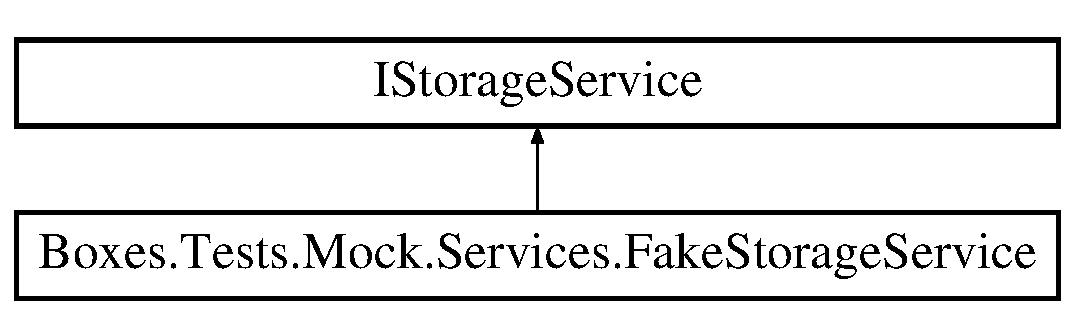
\includegraphics[height=2.000000cm]{class_boxes_1_1_tests_1_1_mock_1_1_services_1_1_fake_storage_service}
\end{center}
\end{figure}
\subsection*{Fonctions membres publiques}
\begin{DoxyCompactItemize}
\item 
\hyperlink{class_boxes_1_1_tests_1_1_mock_1_1_services_1_1_fake_storage_service_a8a290ba0137da5e8f3f30fe90bd870a0}{Fake\+Storage\+Service} ()
\begin{DoxyCompactList}\small\item\em Constructeur non paramétré qui initialise le conteneur fictif de paramètres d\textquotesingle{}application. \end{DoxyCompactList}\item 
void \hyperlink{class_boxes_1_1_tests_1_1_mock_1_1_services_1_1_fake_storage_service_a5f3f15f8bcc6835b7eb956031a59b1d3}{Save\+Setting} (string key, object value)
\item 
T \hyperlink{class_boxes_1_1_tests_1_1_mock_1_1_services_1_1_fake_storage_service_ac4e7fddd7ea20113f45135d2d755bef7}{Read\+Setting$<$ T $>$} (string key)
\item 
void \hyperlink{class_boxes_1_1_tests_1_1_mock_1_1_services_1_1_fake_storage_service_a87e61ad9310b981eb1196624b07a3255}{Remove\+Setting} (string key)
\end{DoxyCompactItemize}
\subsection*{Propriétés}
\begin{DoxyCompactItemize}
\item 
Dictionary$<$ string, object $>$ \hyperlink{class_boxes_1_1_tests_1_1_mock_1_1_services_1_1_fake_storage_service_a9fed901c6df2d7911216314158671caa}{Local\+Settings}\hspace{0.3cm}{\ttfamily  \mbox{[}get, private set\mbox{]}}
\begin{DoxyCompactList}\small\item\em Conteneur fictif de paramètres d\textquotesingle{}application. \end{DoxyCompactList}\end{DoxyCompactItemize}


\subsection{Description détaillée}
Service d\textquotesingle{}accès aux données d\textquotesingle{}un stockage local fictif. 



\subsection{Documentation des constructeurs et destructeur}
\index{Boxes\+::\+Tests\+::\+Mock\+::\+Services\+::\+Fake\+Storage\+Service@{Boxes\+::\+Tests\+::\+Mock\+::\+Services\+::\+Fake\+Storage\+Service}!Fake\+Storage\+Service@{Fake\+Storage\+Service}}
\index{Fake\+Storage\+Service@{Fake\+Storage\+Service}!Boxes\+::\+Tests\+::\+Mock\+::\+Services\+::\+Fake\+Storage\+Service@{Boxes\+::\+Tests\+::\+Mock\+::\+Services\+::\+Fake\+Storage\+Service}}
\subsubsection[{\texorpdfstring{Fake\+Storage\+Service()}{FakeStorageService()}}]{\setlength{\rightskip}{0pt plus 5cm}Boxes.\+Tests.\+Mock.\+Services.\+Fake\+Storage\+Service.\+Fake\+Storage\+Service (
\begin{DoxyParamCaption}
{}
\end{DoxyParamCaption}
)}\hypertarget{class_boxes_1_1_tests_1_1_mock_1_1_services_1_1_fake_storage_service_a8a290ba0137da5e8f3f30fe90bd870a0}{}\label{class_boxes_1_1_tests_1_1_mock_1_1_services_1_1_fake_storage_service_a8a290ba0137da5e8f3f30fe90bd870a0}


Constructeur non paramétré qui initialise le conteneur fictif de paramètres d\textquotesingle{}application. 



\subsection{Documentation des fonctions membres}
\index{Boxes\+::\+Tests\+::\+Mock\+::\+Services\+::\+Fake\+Storage\+Service@{Boxes\+::\+Tests\+::\+Mock\+::\+Services\+::\+Fake\+Storage\+Service}!Read\+Setting$<$ T $>$@{Read\+Setting$<$ T $>$}}
\index{Read\+Setting$<$ T $>$@{Read\+Setting$<$ T $>$}!Boxes\+::\+Tests\+::\+Mock\+::\+Services\+::\+Fake\+Storage\+Service@{Boxes\+::\+Tests\+::\+Mock\+::\+Services\+::\+Fake\+Storage\+Service}}
\subsubsection[{\texorpdfstring{Read\+Setting$<$ T $>$(string key)}{ReadSetting< T >(string key)}}]{\setlength{\rightskip}{0pt plus 5cm}T Boxes.\+Tests.\+Mock.\+Services.\+Fake\+Storage\+Service.\+Read\+Setting$<$ T $>$ (
\begin{DoxyParamCaption}
\item[{string}]{key}
\end{DoxyParamCaption}
)}\hypertarget{class_boxes_1_1_tests_1_1_mock_1_1_services_1_1_fake_storage_service_ac4e7fddd7ea20113f45135d2d755bef7}{}\label{class_boxes_1_1_tests_1_1_mock_1_1_services_1_1_fake_storage_service_ac4e7fddd7ea20113f45135d2d755bef7}




\begin{Desc}
\item[Contraintes de type]\begin{description}
\item[{\em T} : {\em class}]\end{description}
\end{Desc}
\index{Boxes\+::\+Tests\+::\+Mock\+::\+Services\+::\+Fake\+Storage\+Service@{Boxes\+::\+Tests\+::\+Mock\+::\+Services\+::\+Fake\+Storage\+Service}!Remove\+Setting@{Remove\+Setting}}
\index{Remove\+Setting@{Remove\+Setting}!Boxes\+::\+Tests\+::\+Mock\+::\+Services\+::\+Fake\+Storage\+Service@{Boxes\+::\+Tests\+::\+Mock\+::\+Services\+::\+Fake\+Storage\+Service}}
\subsubsection[{\texorpdfstring{Remove\+Setting(string key)}{RemoveSetting(string key)}}]{\setlength{\rightskip}{0pt plus 5cm}void Boxes.\+Tests.\+Mock.\+Services.\+Fake\+Storage\+Service.\+Remove\+Setting (
\begin{DoxyParamCaption}
\item[{string}]{key}
\end{DoxyParamCaption}
)}\hypertarget{class_boxes_1_1_tests_1_1_mock_1_1_services_1_1_fake_storage_service_a87e61ad9310b981eb1196624b07a3255}{}\label{class_boxes_1_1_tests_1_1_mock_1_1_services_1_1_fake_storage_service_a87e61ad9310b981eb1196624b07a3255}




\index{Boxes\+::\+Tests\+::\+Mock\+::\+Services\+::\+Fake\+Storage\+Service@{Boxes\+::\+Tests\+::\+Mock\+::\+Services\+::\+Fake\+Storage\+Service}!Save\+Setting@{Save\+Setting}}
\index{Save\+Setting@{Save\+Setting}!Boxes\+::\+Tests\+::\+Mock\+::\+Services\+::\+Fake\+Storage\+Service@{Boxes\+::\+Tests\+::\+Mock\+::\+Services\+::\+Fake\+Storage\+Service}}
\subsubsection[{\texorpdfstring{Save\+Setting(string key, object value)}{SaveSetting(string key, object value)}}]{\setlength{\rightskip}{0pt plus 5cm}void Boxes.\+Tests.\+Mock.\+Services.\+Fake\+Storage\+Service.\+Save\+Setting (
\begin{DoxyParamCaption}
\item[{string}]{key, }
\item[{object}]{value}
\end{DoxyParamCaption}
)}\hypertarget{class_boxes_1_1_tests_1_1_mock_1_1_services_1_1_fake_storage_service_a5f3f15f8bcc6835b7eb956031a59b1d3}{}\label{class_boxes_1_1_tests_1_1_mock_1_1_services_1_1_fake_storage_service_a5f3f15f8bcc6835b7eb956031a59b1d3}






\subsection{Documentation des propriétés}
\index{Boxes\+::\+Tests\+::\+Mock\+::\+Services\+::\+Fake\+Storage\+Service@{Boxes\+::\+Tests\+::\+Mock\+::\+Services\+::\+Fake\+Storage\+Service}!Local\+Settings@{Local\+Settings}}
\index{Local\+Settings@{Local\+Settings}!Boxes\+::\+Tests\+::\+Mock\+::\+Services\+::\+Fake\+Storage\+Service@{Boxes\+::\+Tests\+::\+Mock\+::\+Services\+::\+Fake\+Storage\+Service}}
\subsubsection[{\texorpdfstring{Local\+Settings}{LocalSettings}}]{\setlength{\rightskip}{0pt plus 5cm}Dictionary$<$string, object$>$ Boxes.\+Tests.\+Mock.\+Services.\+Fake\+Storage\+Service.\+Local\+Settings\hspace{0.3cm}{\ttfamily [get]}, {\ttfamily [private set]}}\hypertarget{class_boxes_1_1_tests_1_1_mock_1_1_services_1_1_fake_storage_service_a9fed901c6df2d7911216314158671caa}{}\label{class_boxes_1_1_tests_1_1_mock_1_1_services_1_1_fake_storage_service_a9fed901c6df2d7911216314158671caa}


Conteneur fictif de paramètres d\textquotesingle{}application. 



La documentation de cette classe a été générée à partir du fichier suivant \+:\begin{DoxyCompactItemize}
\item 
C\+:/\+Users/thoma/\+One\+Drive/\+Documents/\+Visual Studio 2015/\+Projects/\+Boxes/\+Boxes.\+Tests/\+Mock/\+Services/\hyperlink{_fake_storage_service_8cs}{Fake\+Storage\+Service.\+cs}\end{DoxyCompactItemize}

\hypertarget{class_boxes_1_1_tests_1_1_mock_1_1_services_1_1_fake_user_service}{}\section{Référence de la classe Boxes.\+Tests.\+Mock.\+Services.\+Fake\+User\+Service}
\label{class_boxes_1_1_tests_1_1_mock_1_1_services_1_1_fake_user_service}\index{Boxes.\+Tests.\+Mock.\+Services.\+Fake\+User\+Service@{Boxes.\+Tests.\+Mock.\+Services.\+Fake\+User\+Service}}


Service d\textquotesingle{}accès aux données fictives de l\textquotesingle{}entité User.  


Graphe d\textquotesingle{}héritage de Boxes.\+Tests.\+Mock.\+Services.\+Fake\+User\+Service\+:\begin{figure}[H]
\begin{center}
\leavevmode
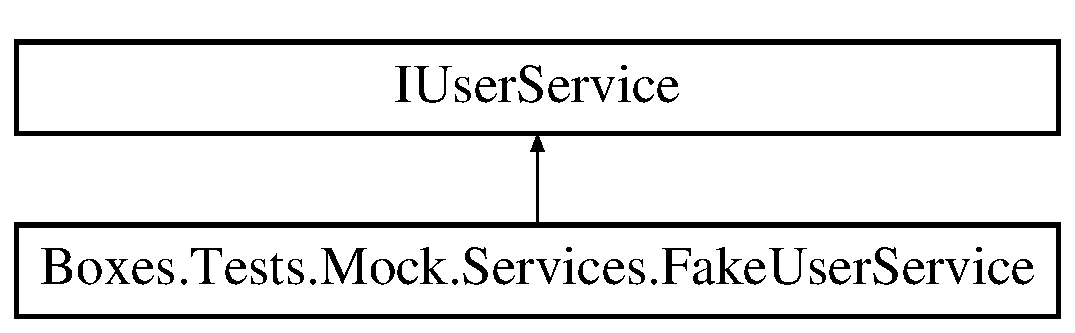
\includegraphics[height=2.000000cm]{class_boxes_1_1_tests_1_1_mock_1_1_services_1_1_fake_user_service}
\end{center}
\end{figure}
\subsection*{Fonctions membres publiques}
\begin{DoxyCompactItemize}
\item 
\hyperlink{class_boxes_1_1_tests_1_1_mock_1_1_services_1_1_fake_user_service_a5b1402a2539d6fd5752c0f25eac9323b}{Fake\+User\+Service} ()
\begin{DoxyCompactList}\small\item\em Constructeur non paramétré qui initialise la liste des utilisateurs fictifs enregistrés en la remplissant. \end{DoxyCompactList}\item 
Task$<$ User $>$ \hyperlink{class_boxes_1_1_tests_1_1_mock_1_1_services_1_1_fake_user_service_a2b5d63cda26573ad15b5d23995fb17fa}{Create\+Async} (User user)
\item 
Task$<$ User $>$ \hyperlink{class_boxes_1_1_tests_1_1_mock_1_1_services_1_1_fake_user_service_a87bb40d334a24116d98982b37232c492}{Get\+By\+Email\+Password\+Async} (string email, string password)
\end{DoxyCompactItemize}
\subsection*{Propriétés}
\begin{DoxyCompactItemize}
\item 
List$<$ User $>$ \hyperlink{class_boxes_1_1_tests_1_1_mock_1_1_services_1_1_fake_user_service_a01b006f8e38195c46cbc92662c80572b}{Users}\hspace{0.3cm}{\ttfamily  \mbox{[}get, private set\mbox{]}}
\begin{DoxyCompactList}\small\item\em Utilisateurs fictifs enregistrés. \end{DoxyCompactList}\end{DoxyCompactItemize}


\subsection{Description détaillée}
Service d\textquotesingle{}accès aux données fictives de l\textquotesingle{}entité User. 



\subsection{Documentation des constructeurs et destructeur}
\index{Boxes\+::\+Tests\+::\+Mock\+::\+Services\+::\+Fake\+User\+Service@{Boxes\+::\+Tests\+::\+Mock\+::\+Services\+::\+Fake\+User\+Service}!Fake\+User\+Service@{Fake\+User\+Service}}
\index{Fake\+User\+Service@{Fake\+User\+Service}!Boxes\+::\+Tests\+::\+Mock\+::\+Services\+::\+Fake\+User\+Service@{Boxes\+::\+Tests\+::\+Mock\+::\+Services\+::\+Fake\+User\+Service}}
\subsubsection[{\texorpdfstring{Fake\+User\+Service()}{FakeUserService()}}]{\setlength{\rightskip}{0pt plus 5cm}Boxes.\+Tests.\+Mock.\+Services.\+Fake\+User\+Service.\+Fake\+User\+Service (
\begin{DoxyParamCaption}
{}
\end{DoxyParamCaption}
)}\hypertarget{class_boxes_1_1_tests_1_1_mock_1_1_services_1_1_fake_user_service_a5b1402a2539d6fd5752c0f25eac9323b}{}\label{class_boxes_1_1_tests_1_1_mock_1_1_services_1_1_fake_user_service_a5b1402a2539d6fd5752c0f25eac9323b}


Constructeur non paramétré qui initialise la liste des utilisateurs fictifs enregistrés en la remplissant. 



\subsection{Documentation des fonctions membres}
\index{Boxes\+::\+Tests\+::\+Mock\+::\+Services\+::\+Fake\+User\+Service@{Boxes\+::\+Tests\+::\+Mock\+::\+Services\+::\+Fake\+User\+Service}!Create\+Async@{Create\+Async}}
\index{Create\+Async@{Create\+Async}!Boxes\+::\+Tests\+::\+Mock\+::\+Services\+::\+Fake\+User\+Service@{Boxes\+::\+Tests\+::\+Mock\+::\+Services\+::\+Fake\+User\+Service}}
\subsubsection[{\texorpdfstring{Create\+Async(\+User user)}{CreateAsync(User user)}}]{\setlength{\rightskip}{0pt plus 5cm}Task$<$User$>$ Boxes.\+Tests.\+Mock.\+Services.\+Fake\+User\+Service.\+Create\+Async (
\begin{DoxyParamCaption}
\item[{User}]{user}
\end{DoxyParamCaption}
)}\hypertarget{class_boxes_1_1_tests_1_1_mock_1_1_services_1_1_fake_user_service_a2b5d63cda26573ad15b5d23995fb17fa}{}\label{class_boxes_1_1_tests_1_1_mock_1_1_services_1_1_fake_user_service_a2b5d63cda26573ad15b5d23995fb17fa}




\index{Boxes\+::\+Tests\+::\+Mock\+::\+Services\+::\+Fake\+User\+Service@{Boxes\+::\+Tests\+::\+Mock\+::\+Services\+::\+Fake\+User\+Service}!Get\+By\+Email\+Password\+Async@{Get\+By\+Email\+Password\+Async}}
\index{Get\+By\+Email\+Password\+Async@{Get\+By\+Email\+Password\+Async}!Boxes\+::\+Tests\+::\+Mock\+::\+Services\+::\+Fake\+User\+Service@{Boxes\+::\+Tests\+::\+Mock\+::\+Services\+::\+Fake\+User\+Service}}
\subsubsection[{\texorpdfstring{Get\+By\+Email\+Password\+Async(string email, string password)}{GetByEmailPasswordAsync(string email, string password)}}]{\setlength{\rightskip}{0pt plus 5cm}Task$<$User$>$ Boxes.\+Tests.\+Mock.\+Services.\+Fake\+User\+Service.\+Get\+By\+Email\+Password\+Async (
\begin{DoxyParamCaption}
\item[{string}]{email, }
\item[{string}]{password}
\end{DoxyParamCaption}
)}\hypertarget{class_boxes_1_1_tests_1_1_mock_1_1_services_1_1_fake_user_service_a87bb40d334a24116d98982b37232c492}{}\label{class_boxes_1_1_tests_1_1_mock_1_1_services_1_1_fake_user_service_a87bb40d334a24116d98982b37232c492}






\subsection{Documentation des propriétés}
\index{Boxes\+::\+Tests\+::\+Mock\+::\+Services\+::\+Fake\+User\+Service@{Boxes\+::\+Tests\+::\+Mock\+::\+Services\+::\+Fake\+User\+Service}!Users@{Users}}
\index{Users@{Users}!Boxes\+::\+Tests\+::\+Mock\+::\+Services\+::\+Fake\+User\+Service@{Boxes\+::\+Tests\+::\+Mock\+::\+Services\+::\+Fake\+User\+Service}}
\subsubsection[{\texorpdfstring{Users}{Users}}]{\setlength{\rightskip}{0pt plus 5cm}List$<$User$>$ Boxes.\+Tests.\+Mock.\+Services.\+Fake\+User\+Service.\+Users\hspace{0.3cm}{\ttfamily [get]}, {\ttfamily [private set]}}\hypertarget{class_boxes_1_1_tests_1_1_mock_1_1_services_1_1_fake_user_service_a01b006f8e38195c46cbc92662c80572b}{}\label{class_boxes_1_1_tests_1_1_mock_1_1_services_1_1_fake_user_service_a01b006f8e38195c46cbc92662c80572b}


Utilisateurs fictifs enregistrés. 



La documentation de cette classe a été générée à partir du fichier suivant \+:\begin{DoxyCompactItemize}
\item 
C\+:/\+Users/thoma/\+One\+Drive/\+Documents/\+Visual Studio 2015/\+Projects/\+Boxes/\+Boxes.\+Tests/\+Mock/\+Services/\hyperlink{_fake_user_service_8cs}{Fake\+User\+Service.\+cs}\end{DoxyCompactItemize}

\hypertarget{class_boxes_1_1_tests_1_1_home_view_model_tests}{}\section{Référence de la classe Boxes.\+Tests.\+Home\+View\+Model\+Tests}
\label{class_boxes_1_1_tests_1_1_home_view_model_tests}\index{Boxes.\+Tests.\+Home\+View\+Model\+Tests@{Boxes.\+Tests.\+Home\+View\+Model\+Tests}}


Effectue les tests unitaires relatifs au view model Home\+View\+Model.  


\subsection*{Fonctions membres publiques}
\begin{DoxyCompactItemize}
\item 
void \hyperlink{class_boxes_1_1_tests_1_1_home_view_model_tests_a9961c9ccfb49e506ee4c3e9f625386e1}{Tests\+Initialize} ()
\begin{DoxyCompactList}\small\item\em Effectue les initialisation qui doivent s\textquotesingle{}exécuter avant chaque test. \end{DoxyCompactList}\item 
void \hyperlink{class_boxes_1_1_tests_1_1_home_view_model_tests_a2b014e6e0e790f691c0bf6e939e6ad34}{Tests\+Cleanup} ()
\begin{DoxyCompactList}\small\item\em Effectue les nettoyages de variables devant être faits après l\textquotesingle{}exécution de chaque test. \end{DoxyCompactList}\item 
async Task \hyperlink{class_boxes_1_1_tests_1_1_home_view_model_tests_a4a49b19e1b9bd1feb12cf22e22fcfe63}{Initialize\+\_\+\+Navigation\+To\+Home\+\_\+\+Posts\+Not\+Empty} ()
\begin{DoxyCompactList}\small\item\em Vérifie que lorsque l\textquotesingle{}utilisateur entre sur la page d\textquotesingle{}accueil, la propriété {\ttfamily Posts} du view model de cette page ne soit pas une collection vide. \end{DoxyCompactList}\item 
void \hyperlink{class_boxes_1_1_tests_1_1_home_view_model_tests_aa687cb2dc81e032dd75c74e7b59fc549}{Initialize\+\_\+\+Navigation\+To\+Home\+\_\+\+Shell\+Title\+Message\+Sent} ()
\begin{DoxyCompactList}\small\item\em Vérifie que lorsque l\textquotesingle{}utilisateur entre sur la page d\textquotesingle{}accuei, un message de type Shell\+Title\+Message est envoyé afin de demander le changement du titre du shell. \end{DoxyCompactList}\item 
void \hyperlink{class_boxes_1_1_tests_1_1_home_view_model_tests_aa78160a21f8b66a83ed7274623d0abcb}{Show\+Post\+Command\+\_\+\+Go\+To\+Post\+Page\+\_\+\+Current\+Page\+Is\+Post} ()
\begin{DoxyCompactList}\small\item\em Vérifie que lorsque l\textquotesingle{}utilisateur veut voir le détail d\textquotesingle{}un post et appel ainsi la commande d\textquotesingle{}affichage d\textquotesingle{}un post, la page actuellement affichée est celle de ce post. \end{DoxyCompactList}\item 
void \hyperlink{class_boxes_1_1_tests_1_1_home_view_model_tests_a2dad74f03a4ec9a258d8c2bc1e8f17fc}{Show\+Post\+Command\+\_\+\+Go\+To\+Post\+Page\+\_\+\+Current\+Page\+Parameter\+Is\+Post\+To\+Show} ()
\begin{DoxyCompactList}\small\item\em Vérifie que lorsque l\textquotesingle{}utilisateur veut voir le détail d\textquotesingle{}un post et appel ainsi la commande d\textquotesingle{}affichage d\textquotesingle{}un post, le paramètre de la page actuellement affichée est bien le post à afficher. \end{DoxyCompactList}\end{DoxyCompactItemize}
\subsection*{Fonctions membres publiques statiques}
\begin{DoxyCompactItemize}
\item 
static void \hyperlink{class_boxes_1_1_tests_1_1_home_view_model_tests_ad36d1ae9e993528529648a43bf1ec5f3}{Class\+Initialize} (Test\+Context context)
\begin{DoxyCompactList}\small\item\em Effectue les initialisation qui doivent être faites avant l\textquotesingle{}exécution du premier test. \end{DoxyCompactList}\item 
static void \hyperlink{class_boxes_1_1_tests_1_1_home_view_model_tests_ada2e3c534138168cb082be5b6155033e}{Class\+Cleanup} ()
\begin{DoxyCompactList}\small\item\em Effectue les nettoyages qui doivent être faits après l\textquotesingle{}exécution du dernier test. \end{DoxyCompactList}\end{DoxyCompactItemize}
\subsection*{Attributs privés}
\begin{DoxyCompactItemize}
\item 
\hyperlink{class_boxes_1_1_tests_1_1_mock_1_1_services_1_1_fake_storage_service}{Fake\+Storage\+Service} \hyperlink{class_boxes_1_1_tests_1_1_home_view_model_tests_a3cef168c7e8bcdbee02a6713e4541105}{storage\+Service}
\begin{DoxyCompactList}\small\item\em Stock le service d\textquotesingle{}accès aux données fictives de stockage local. \end{DoxyCompactList}\item 
\hyperlink{class_boxes_1_1_tests_1_1_mock_1_1_services_1_1_fake_navigation_service}{Fake\+Navigation\+Service} \hyperlink{class_boxes_1_1_tests_1_1_home_view_model_tests_aa4981a7ac7b616762cfc1703b52c42d1}{navigation\+Service}
\begin{DoxyCompactList}\small\item\em Stock le service de navigation fictive. \end{DoxyCompactList}\item 
\hyperlink{class_boxes_1_1_tests_1_1_mock_1_1_services_1_1_fake_post_service}{Fake\+Post\+Service} \hyperlink{class_boxes_1_1_tests_1_1_home_view_model_tests_a2bfaed74f121657195e437b0dfca8eb2}{post\+Service}
\begin{DoxyCompactList}\small\item\em Stock le service d\textquotesingle{}accès aux données fictives de l\textquotesingle{}entité Post. \end{DoxyCompactList}\item 
\hyperlink{class_boxes_1_1_tests_1_1_mock_1_1_services_1_1_fake_localization_service}{Fake\+Localization\+Service} \hyperlink{class_boxes_1_1_tests_1_1_home_view_model_tests_a0451d15ae4b229db13798e8c6ddd966f}{localization\+Service}
\begin{DoxyCompactList}\small\item\em Stock le service d\textquotesingle{}accès aux données fictives de localization. \end{DoxyCompactList}\item 
Home\+View\+Model \hyperlink{class_boxes_1_1_tests_1_1_home_view_model_tests_a5e19b63ded52862d0545d317fc2406e0}{home\+View\+Model}
\begin{DoxyCompactList}\small\item\em Stock le view model de la page d\textquotesingle{}accueil (ici le view model à tester). \end{DoxyCompactList}\end{DoxyCompactItemize}
\subsection*{Attributs privés statiques}
\begin{DoxyCompactItemize}
\item 
static Random \hyperlink{class_boxes_1_1_tests_1_1_home_view_model_tests_aa651dd64428e19075fded9c393db63c3}{random}
\begin{DoxyCompactList}\small\item\em Stock l\textquotesingle{}objet de génération de nombres aléatoires. \end{DoxyCompactList}\end{DoxyCompactItemize}


\subsection{Description détaillée}
Effectue les tests unitaires relatifs au view model Home\+View\+Model. 



\subsection{Documentation des fonctions membres}
\index{Boxes\+::\+Tests\+::\+Home\+View\+Model\+Tests@{Boxes\+::\+Tests\+::\+Home\+View\+Model\+Tests}!Class\+Cleanup@{Class\+Cleanup}}
\index{Class\+Cleanup@{Class\+Cleanup}!Boxes\+::\+Tests\+::\+Home\+View\+Model\+Tests@{Boxes\+::\+Tests\+::\+Home\+View\+Model\+Tests}}
\subsubsection[{\texorpdfstring{Class\+Cleanup()}{ClassCleanup()}}]{\setlength{\rightskip}{0pt plus 5cm}static void Boxes.\+Tests.\+Home\+View\+Model\+Tests.\+Class\+Cleanup (
\begin{DoxyParamCaption}
{}
\end{DoxyParamCaption}
)\hspace{0.3cm}{\ttfamily [static]}}\hypertarget{class_boxes_1_1_tests_1_1_home_view_model_tests_ada2e3c534138168cb082be5b6155033e}{}\label{class_boxes_1_1_tests_1_1_home_view_model_tests_ada2e3c534138168cb082be5b6155033e}


Effectue les nettoyages qui doivent être faits après l\textquotesingle{}exécution du dernier test. 

\index{Boxes\+::\+Tests\+::\+Home\+View\+Model\+Tests@{Boxes\+::\+Tests\+::\+Home\+View\+Model\+Tests}!Class\+Initialize@{Class\+Initialize}}
\index{Class\+Initialize@{Class\+Initialize}!Boxes\+::\+Tests\+::\+Home\+View\+Model\+Tests@{Boxes\+::\+Tests\+::\+Home\+View\+Model\+Tests}}
\subsubsection[{\texorpdfstring{Class\+Initialize(\+Test\+Context context)}{ClassInitialize(TestContext context)}}]{\setlength{\rightskip}{0pt plus 5cm}static void Boxes.\+Tests.\+Home\+View\+Model\+Tests.\+Class\+Initialize (
\begin{DoxyParamCaption}
\item[{Test\+Context}]{context}
\end{DoxyParamCaption}
)\hspace{0.3cm}{\ttfamily [static]}}\hypertarget{class_boxes_1_1_tests_1_1_home_view_model_tests_ad36d1ae9e993528529648a43bf1ec5f3}{}\label{class_boxes_1_1_tests_1_1_home_view_model_tests_ad36d1ae9e993528529648a43bf1ec5f3}


Effectue les initialisation qui doivent être faites avant l\textquotesingle{}exécution du premier test. 

\index{Boxes\+::\+Tests\+::\+Home\+View\+Model\+Tests@{Boxes\+::\+Tests\+::\+Home\+View\+Model\+Tests}!Initialize\+\_\+\+Navigation\+To\+Home\+\_\+\+Posts\+Not\+Empty@{Initialize\+\_\+\+Navigation\+To\+Home\+\_\+\+Posts\+Not\+Empty}}
\index{Initialize\+\_\+\+Navigation\+To\+Home\+\_\+\+Posts\+Not\+Empty@{Initialize\+\_\+\+Navigation\+To\+Home\+\_\+\+Posts\+Not\+Empty}!Boxes\+::\+Tests\+::\+Home\+View\+Model\+Tests@{Boxes\+::\+Tests\+::\+Home\+View\+Model\+Tests}}
\subsubsection[{\texorpdfstring{Initialize\+\_\+\+Navigation\+To\+Home\+\_\+\+Posts\+Not\+Empty()}{Initialize_NavigationToHome_PostsNotEmpty()}}]{\setlength{\rightskip}{0pt plus 5cm}async Task Boxes.\+Tests.\+Home\+View\+Model\+Tests.\+Initialize\+\_\+\+Navigation\+To\+Home\+\_\+\+Posts\+Not\+Empty (
\begin{DoxyParamCaption}
{}
\end{DoxyParamCaption}
)}\hypertarget{class_boxes_1_1_tests_1_1_home_view_model_tests_a4a49b19e1b9bd1feb12cf22e22fcfe63}{}\label{class_boxes_1_1_tests_1_1_home_view_model_tests_a4a49b19e1b9bd1feb12cf22e22fcfe63}


Vérifie que lorsque l\textquotesingle{}utilisateur entre sur la page d\textquotesingle{}accueil, la propriété {\ttfamily Posts} du view model de cette page ne soit pas une collection vide. 

\begin{DoxyReturn}{Renvoie}
Tache asynchrone qui permet d\textquotesingle{}attendre la fin des opérations. 
\end{DoxyReturn}
\index{Boxes\+::\+Tests\+::\+Home\+View\+Model\+Tests@{Boxes\+::\+Tests\+::\+Home\+View\+Model\+Tests}!Initialize\+\_\+\+Navigation\+To\+Home\+\_\+\+Shell\+Title\+Message\+Sent@{Initialize\+\_\+\+Navigation\+To\+Home\+\_\+\+Shell\+Title\+Message\+Sent}}
\index{Initialize\+\_\+\+Navigation\+To\+Home\+\_\+\+Shell\+Title\+Message\+Sent@{Initialize\+\_\+\+Navigation\+To\+Home\+\_\+\+Shell\+Title\+Message\+Sent}!Boxes\+::\+Tests\+::\+Home\+View\+Model\+Tests@{Boxes\+::\+Tests\+::\+Home\+View\+Model\+Tests}}
\subsubsection[{\texorpdfstring{Initialize\+\_\+\+Navigation\+To\+Home\+\_\+\+Shell\+Title\+Message\+Sent()}{Initialize_NavigationToHome_ShellTitleMessageSent()}}]{\setlength{\rightskip}{0pt plus 5cm}void Boxes.\+Tests.\+Home\+View\+Model\+Tests.\+Initialize\+\_\+\+Navigation\+To\+Home\+\_\+\+Shell\+Title\+Message\+Sent (
\begin{DoxyParamCaption}
{}
\end{DoxyParamCaption}
)}\hypertarget{class_boxes_1_1_tests_1_1_home_view_model_tests_aa687cb2dc81e032dd75c74e7b59fc549}{}\label{class_boxes_1_1_tests_1_1_home_view_model_tests_aa687cb2dc81e032dd75c74e7b59fc549}


Vérifie que lorsque l\textquotesingle{}utilisateur entre sur la page d\textquotesingle{}accuei, un message de type Shell\+Title\+Message est envoyé afin de demander le changement du titre du shell. 

\index{Boxes\+::\+Tests\+::\+Home\+View\+Model\+Tests@{Boxes\+::\+Tests\+::\+Home\+View\+Model\+Tests}!Show\+Post\+Command\+\_\+\+Go\+To\+Post\+Page\+\_\+\+Current\+Page\+Is\+Post@{Show\+Post\+Command\+\_\+\+Go\+To\+Post\+Page\+\_\+\+Current\+Page\+Is\+Post}}
\index{Show\+Post\+Command\+\_\+\+Go\+To\+Post\+Page\+\_\+\+Current\+Page\+Is\+Post@{Show\+Post\+Command\+\_\+\+Go\+To\+Post\+Page\+\_\+\+Current\+Page\+Is\+Post}!Boxes\+::\+Tests\+::\+Home\+View\+Model\+Tests@{Boxes\+::\+Tests\+::\+Home\+View\+Model\+Tests}}
\subsubsection[{\texorpdfstring{Show\+Post\+Command\+\_\+\+Go\+To\+Post\+Page\+\_\+\+Current\+Page\+Is\+Post()}{ShowPostCommand_GoToPostPage_CurrentPageIsPost()}}]{\setlength{\rightskip}{0pt plus 5cm}void Boxes.\+Tests.\+Home\+View\+Model\+Tests.\+Show\+Post\+Command\+\_\+\+Go\+To\+Post\+Page\+\_\+\+Current\+Page\+Is\+Post (
\begin{DoxyParamCaption}
{}
\end{DoxyParamCaption}
)}\hypertarget{class_boxes_1_1_tests_1_1_home_view_model_tests_aa78160a21f8b66a83ed7274623d0abcb}{}\label{class_boxes_1_1_tests_1_1_home_view_model_tests_aa78160a21f8b66a83ed7274623d0abcb}


Vérifie que lorsque l\textquotesingle{}utilisateur veut voir le détail d\textquotesingle{}un post et appel ainsi la commande d\textquotesingle{}affichage d\textquotesingle{}un post, la page actuellement affichée est celle de ce post. 

\index{Boxes\+::\+Tests\+::\+Home\+View\+Model\+Tests@{Boxes\+::\+Tests\+::\+Home\+View\+Model\+Tests}!Show\+Post\+Command\+\_\+\+Go\+To\+Post\+Page\+\_\+\+Current\+Page\+Parameter\+Is\+Post\+To\+Show@{Show\+Post\+Command\+\_\+\+Go\+To\+Post\+Page\+\_\+\+Current\+Page\+Parameter\+Is\+Post\+To\+Show}}
\index{Show\+Post\+Command\+\_\+\+Go\+To\+Post\+Page\+\_\+\+Current\+Page\+Parameter\+Is\+Post\+To\+Show@{Show\+Post\+Command\+\_\+\+Go\+To\+Post\+Page\+\_\+\+Current\+Page\+Parameter\+Is\+Post\+To\+Show}!Boxes\+::\+Tests\+::\+Home\+View\+Model\+Tests@{Boxes\+::\+Tests\+::\+Home\+View\+Model\+Tests}}
\subsubsection[{\texorpdfstring{Show\+Post\+Command\+\_\+\+Go\+To\+Post\+Page\+\_\+\+Current\+Page\+Parameter\+Is\+Post\+To\+Show()}{ShowPostCommand_GoToPostPage_CurrentPageParameterIsPostToShow()}}]{\setlength{\rightskip}{0pt plus 5cm}void Boxes.\+Tests.\+Home\+View\+Model\+Tests.\+Show\+Post\+Command\+\_\+\+Go\+To\+Post\+Page\+\_\+\+Current\+Page\+Parameter\+Is\+Post\+To\+Show (
\begin{DoxyParamCaption}
{}
\end{DoxyParamCaption}
)}\hypertarget{class_boxes_1_1_tests_1_1_home_view_model_tests_a2dad74f03a4ec9a258d8c2bc1e8f17fc}{}\label{class_boxes_1_1_tests_1_1_home_view_model_tests_a2dad74f03a4ec9a258d8c2bc1e8f17fc}


Vérifie que lorsque l\textquotesingle{}utilisateur veut voir le détail d\textquotesingle{}un post et appel ainsi la commande d\textquotesingle{}affichage d\textquotesingle{}un post, le paramètre de la page actuellement affichée est bien le post à afficher. 

\index{Boxes\+::\+Tests\+::\+Home\+View\+Model\+Tests@{Boxes\+::\+Tests\+::\+Home\+View\+Model\+Tests}!Tests\+Cleanup@{Tests\+Cleanup}}
\index{Tests\+Cleanup@{Tests\+Cleanup}!Boxes\+::\+Tests\+::\+Home\+View\+Model\+Tests@{Boxes\+::\+Tests\+::\+Home\+View\+Model\+Tests}}
\subsubsection[{\texorpdfstring{Tests\+Cleanup()}{TestsCleanup()}}]{\setlength{\rightskip}{0pt plus 5cm}void Boxes.\+Tests.\+Home\+View\+Model\+Tests.\+Tests\+Cleanup (
\begin{DoxyParamCaption}
{}
\end{DoxyParamCaption}
)}\hypertarget{class_boxes_1_1_tests_1_1_home_view_model_tests_a2b014e6e0e790f691c0bf6e939e6ad34}{}\label{class_boxes_1_1_tests_1_1_home_view_model_tests_a2b014e6e0e790f691c0bf6e939e6ad34}


Effectue les nettoyages de variables devant être faits après l\textquotesingle{}exécution de chaque test. 

\index{Boxes\+::\+Tests\+::\+Home\+View\+Model\+Tests@{Boxes\+::\+Tests\+::\+Home\+View\+Model\+Tests}!Tests\+Initialize@{Tests\+Initialize}}
\index{Tests\+Initialize@{Tests\+Initialize}!Boxes\+::\+Tests\+::\+Home\+View\+Model\+Tests@{Boxes\+::\+Tests\+::\+Home\+View\+Model\+Tests}}
\subsubsection[{\texorpdfstring{Tests\+Initialize()}{TestsInitialize()}}]{\setlength{\rightskip}{0pt plus 5cm}void Boxes.\+Tests.\+Home\+View\+Model\+Tests.\+Tests\+Initialize (
\begin{DoxyParamCaption}
{}
\end{DoxyParamCaption}
)}\hypertarget{class_boxes_1_1_tests_1_1_home_view_model_tests_a9961c9ccfb49e506ee4c3e9f625386e1}{}\label{class_boxes_1_1_tests_1_1_home_view_model_tests_a9961c9ccfb49e506ee4c3e9f625386e1}


Effectue les initialisation qui doivent s\textquotesingle{}exécuter avant chaque test. 



\subsection{Documentation des données membres}
\index{Boxes\+::\+Tests\+::\+Home\+View\+Model\+Tests@{Boxes\+::\+Tests\+::\+Home\+View\+Model\+Tests}!home\+View\+Model@{home\+View\+Model}}
\index{home\+View\+Model@{home\+View\+Model}!Boxes\+::\+Tests\+::\+Home\+View\+Model\+Tests@{Boxes\+::\+Tests\+::\+Home\+View\+Model\+Tests}}
\subsubsection[{\texorpdfstring{home\+View\+Model}{homeViewModel}}]{\setlength{\rightskip}{0pt plus 5cm}Home\+View\+Model Boxes.\+Tests.\+Home\+View\+Model\+Tests.\+home\+View\+Model\hspace{0.3cm}{\ttfamily [private]}}\hypertarget{class_boxes_1_1_tests_1_1_home_view_model_tests_a5e19b63ded52862d0545d317fc2406e0}{}\label{class_boxes_1_1_tests_1_1_home_view_model_tests_a5e19b63ded52862d0545d317fc2406e0}


Stock le view model de la page d\textquotesingle{}accueil (ici le view model à tester). 

\index{Boxes\+::\+Tests\+::\+Home\+View\+Model\+Tests@{Boxes\+::\+Tests\+::\+Home\+View\+Model\+Tests}!localization\+Service@{localization\+Service}}
\index{localization\+Service@{localization\+Service}!Boxes\+::\+Tests\+::\+Home\+View\+Model\+Tests@{Boxes\+::\+Tests\+::\+Home\+View\+Model\+Tests}}
\subsubsection[{\texorpdfstring{localization\+Service}{localizationService}}]{\setlength{\rightskip}{0pt plus 5cm}{\bf Fake\+Localization\+Service} Boxes.\+Tests.\+Home\+View\+Model\+Tests.\+localization\+Service\hspace{0.3cm}{\ttfamily [private]}}\hypertarget{class_boxes_1_1_tests_1_1_home_view_model_tests_a0451d15ae4b229db13798e8c6ddd966f}{}\label{class_boxes_1_1_tests_1_1_home_view_model_tests_a0451d15ae4b229db13798e8c6ddd966f}


Stock le service d\textquotesingle{}accès aux données fictives de localization. 

\index{Boxes\+::\+Tests\+::\+Home\+View\+Model\+Tests@{Boxes\+::\+Tests\+::\+Home\+View\+Model\+Tests}!navigation\+Service@{navigation\+Service}}
\index{navigation\+Service@{navigation\+Service}!Boxes\+::\+Tests\+::\+Home\+View\+Model\+Tests@{Boxes\+::\+Tests\+::\+Home\+View\+Model\+Tests}}
\subsubsection[{\texorpdfstring{navigation\+Service}{navigationService}}]{\setlength{\rightskip}{0pt plus 5cm}{\bf Fake\+Navigation\+Service} Boxes.\+Tests.\+Home\+View\+Model\+Tests.\+navigation\+Service\hspace{0.3cm}{\ttfamily [private]}}\hypertarget{class_boxes_1_1_tests_1_1_home_view_model_tests_aa4981a7ac7b616762cfc1703b52c42d1}{}\label{class_boxes_1_1_tests_1_1_home_view_model_tests_aa4981a7ac7b616762cfc1703b52c42d1}


Stock le service de navigation fictive. 

\index{Boxes\+::\+Tests\+::\+Home\+View\+Model\+Tests@{Boxes\+::\+Tests\+::\+Home\+View\+Model\+Tests}!post\+Service@{post\+Service}}
\index{post\+Service@{post\+Service}!Boxes\+::\+Tests\+::\+Home\+View\+Model\+Tests@{Boxes\+::\+Tests\+::\+Home\+View\+Model\+Tests}}
\subsubsection[{\texorpdfstring{post\+Service}{postService}}]{\setlength{\rightskip}{0pt plus 5cm}{\bf Fake\+Post\+Service} Boxes.\+Tests.\+Home\+View\+Model\+Tests.\+post\+Service\hspace{0.3cm}{\ttfamily [private]}}\hypertarget{class_boxes_1_1_tests_1_1_home_view_model_tests_a2bfaed74f121657195e437b0dfca8eb2}{}\label{class_boxes_1_1_tests_1_1_home_view_model_tests_a2bfaed74f121657195e437b0dfca8eb2}


Stock le service d\textquotesingle{}accès aux données fictives de l\textquotesingle{}entité Post. 

\index{Boxes\+::\+Tests\+::\+Home\+View\+Model\+Tests@{Boxes\+::\+Tests\+::\+Home\+View\+Model\+Tests}!random@{random}}
\index{random@{random}!Boxes\+::\+Tests\+::\+Home\+View\+Model\+Tests@{Boxes\+::\+Tests\+::\+Home\+View\+Model\+Tests}}
\subsubsection[{\texorpdfstring{random}{random}}]{\setlength{\rightskip}{0pt plus 5cm}Random Boxes.\+Tests.\+Home\+View\+Model\+Tests.\+random\hspace{0.3cm}{\ttfamily [static]}, {\ttfamily [private]}}\hypertarget{class_boxes_1_1_tests_1_1_home_view_model_tests_aa651dd64428e19075fded9c393db63c3}{}\label{class_boxes_1_1_tests_1_1_home_view_model_tests_aa651dd64428e19075fded9c393db63c3}


Stock l\textquotesingle{}objet de génération de nombres aléatoires. 

\index{Boxes\+::\+Tests\+::\+Home\+View\+Model\+Tests@{Boxes\+::\+Tests\+::\+Home\+View\+Model\+Tests}!storage\+Service@{storage\+Service}}
\index{storage\+Service@{storage\+Service}!Boxes\+::\+Tests\+::\+Home\+View\+Model\+Tests@{Boxes\+::\+Tests\+::\+Home\+View\+Model\+Tests}}
\subsubsection[{\texorpdfstring{storage\+Service}{storageService}}]{\setlength{\rightskip}{0pt plus 5cm}{\bf Fake\+Storage\+Service} Boxes.\+Tests.\+Home\+View\+Model\+Tests.\+storage\+Service\hspace{0.3cm}{\ttfamily [private]}}\hypertarget{class_boxes_1_1_tests_1_1_home_view_model_tests_a3cef168c7e8bcdbee02a6713e4541105}{}\label{class_boxes_1_1_tests_1_1_home_view_model_tests_a3cef168c7e8bcdbee02a6713e4541105}


Stock le service d\textquotesingle{}accès aux données fictives de stockage local. 



La documentation de cette classe a été générée à partir du fichier suivant \+:\begin{DoxyCompactItemize}
\item 
C\+:/\+Users/thoma/\+One\+Drive/\+Documents/\+Visual Studio 2015/\+Projects/\+Boxes/\+Boxes.\+Tests/\hyperlink{_home_view_model_tests_8cs}{Home\+View\+Model\+Tests.\+cs}\end{DoxyCompactItemize}

\hypertarget{class_boxes_1_1_tests_1_1_login_view_model_tests}{}\section{Référence de la classe Boxes.\+Tests.\+Login\+View\+Model\+Tests}
\label{class_boxes_1_1_tests_1_1_login_view_model_tests}\index{Boxes.\+Tests.\+Login\+View\+Model\+Tests@{Boxes.\+Tests.\+Login\+View\+Model\+Tests}}


Effectue les tests unitaires qui concernent le Login\+View\+Model.  


\subsection*{Fonctions membres publiques}
\begin{DoxyCompactItemize}
\item 
void \hyperlink{class_boxes_1_1_tests_1_1_login_view_model_tests_aeba1576989bbe4a128a96eff58ff1ee4}{Tests\+Initialize} ()
\begin{DoxyCompactList}\small\item\em Effectue les initialisation qui doivent être exécutées avant l\textquotesingle{}exécution de chaque test. \end{DoxyCompactList}\item 
void \hyperlink{class_boxes_1_1_tests_1_1_login_view_model_tests_a284439b5f36f9b6bb4eb1561bce15c8a}{Tests\+Clean\+Up} ()
\begin{DoxyCompactList}\small\item\em Effectue les nettoyages de variables devant être faits après l\textquotesingle{}exécution de chaque test. \end{DoxyCompactList}\item 
void \hyperlink{class_boxes_1_1_tests_1_1_login_view_model_tests_af7348cc41eeafb8d50c913c5d5cb86cb}{Cleanup\+\_\+\+Navigation\+From\+Login\+\_\+\+Email\+Is\+Null} ()
\begin{DoxyCompactList}\small\item\em Vérifie que lorsque l\textquotesingle{}utilisateur effectue une navigation à partir de la page de connexion, le champ \char`\"{}\+Adresse email\char`\"{} est bien vidé. \end{DoxyCompactList}\item 
void \hyperlink{class_boxes_1_1_tests_1_1_login_view_model_tests_aed742d452397322885bea88dcbd9e2d7}{Cleanup\+\_\+\+Navigation\+From\+Login\+\_\+\+Password\+Is\+Null} ()
\begin{DoxyCompactList}\small\item\em Vérifie que lorsque l\textquotesingle{}utilisateur effectue une navigation à partir de la page de connexion, le champ \char`\"{}\+Mot de passe\char`\"{} est bien vidé. \end{DoxyCompactList}\item 
void \hyperlink{class_boxes_1_1_tests_1_1_login_view_model_tests_a1a1911464b163f9ab6b397dced5de134}{Login\+Command\+\_\+\+Email\+Is\+Null\+Or\+White\+Space\+\_\+\+Cannot\+Execute} (string email)
\begin{DoxyCompactList}\small\item\em Vérifie que lorsque l\textquotesingle{}utilisateur n\textquotesingle{}entre pas d\textquotesingle{}adresse email, la commande de connexion ne peut s\textquotesingle{}exécuter. \end{DoxyCompactList}\item 
void \hyperlink{class_boxes_1_1_tests_1_1_login_view_model_tests_a04afc4b49a9c2877a36dbecadf8c28be}{Login\+Command\+\_\+\+Password\+Is\+Null\+Or\+White\+Space\+\_\+\+Cannot\+Execute} (string password)
\begin{DoxyCompactList}\small\item\em Vérifie que lorsque l\textquotesingle{}utilisateur n\textquotesingle{}entre pas de mot de passe, la commande de connexion ne peut s\textquotesingle{}exécuter. \end{DoxyCompactList}\item 
void \hyperlink{class_boxes_1_1_tests_1_1_login_view_model_tests_aee9eda2825bf6e1f0fd3476c75482672}{Login\+Command\+\_\+\+Is\+Logging\+In\+\_\+\+Cannot\+Execute} ()
\begin{DoxyCompactList}\small\item\em Vérifie que lorsque la connexion de l\textquotesingle{}utilisateur est en cours, la commande de connexion ne peut s\textquotesingle{}exécuter. \end{DoxyCompactList}\item 
void \hyperlink{class_boxes_1_1_tests_1_1_login_view_model_tests_a28a278906bde25013a2f138046a63981}{Login\+Command\+\_\+\+Is\+Not\+Logging\+In\+Email\+Password\+Not\+Null\+Or\+White\+Space\+\_\+\+Can\+Execute} ()
\begin{DoxyCompactList}\small\item\em Vérifie que lorsque la connexion de l\textquotesingle{}utilisateur n\textquotesingle{}est pas en cours et que ce dernier a entré une adresse email et un mot de passe, la commande de connexion peut s\textquotesingle{}exécuter. \end{DoxyCompactList}\item 
async Task \hyperlink{class_boxes_1_1_tests_1_1_login_view_model_tests_aa4e2393650da2c3def7375d8dac4b061}{Login\+Command\+\_\+\+Correct\+Email\+Wrong\+Password\+\_\+\+Current\+Page\+Is\+Login} ()
\begin{DoxyCompactList}\small\item\em Vérifie que lorsque l\textquotesingle{}utilisateur entre une adresse email qui existe mais un mot de passe incorrect, la page actuellement affichée est toujours la page de connexion. \end{DoxyCompactList}\item 
async Task \hyperlink{class_boxes_1_1_tests_1_1_login_view_model_tests_a2fb23554feb022458a5018736f4ce647}{Login\+Command\+\_\+\+Correct\+Email\+Wrong\+Password\+\_\+\+User\+Not\+In\+Local\+Settings} ()
\begin{DoxyCompactList}\small\item\em Vérifie que lorsque l\textquotesingle{}utilisateur entre une adresse email qui existe mais un mot de passe incorrect, aucun utilisateur n\textquotesingle{}est inscrit dans le conteneur de paramètre d\textquotesingle{}application. \end{DoxyCompactList}\item 
async Task \hyperlink{class_boxes_1_1_tests_1_1_login_view_model_tests_a2a1127de3f6d7a127c1e8988a6b9cd9d}{Login\+Command\+\_\+\+Correct\+Email\+Wrong\+Password\+\_\+\+Generic\+Error\+Message\+Sent} ()
\begin{DoxyCompactList}\small\item\em Vérifie que lorsque l\textquotesingle{}utilisateur entre une adresse email qui existe mais un mot de passe incorrect, un message d\textquotesingle{}erreur est envoyé. \end{DoxyCompactList}\item 
async Task \hyperlink{class_boxes_1_1_tests_1_1_login_view_model_tests_ad0a8d68e805d64ee8a8f35ccd071f9e3}{Login\+Command\+\_\+\+Correct\+Email\+Correct\+Password\+\_\+\+User\+In\+Local\+Settings} ()
\begin{DoxyCompactList}\small\item\em Vérifie que lorsque l\textquotesingle{}utilisateur entre une adresse email qui existe et le mot de passe correspondant, celui-\/ci est inscrit dans le conteneur de paramètres d\textquotesingle{}application. \end{DoxyCompactList}\item 
async Task \hyperlink{class_boxes_1_1_tests_1_1_login_view_model_tests_ac6bd2bd039243bef7c8359b762c476d1}{Login\+Command\+\_\+\+Correct\+Email\+Correct\+Password\+\_\+\+Current\+Page\+Is\+Shell} ()
\begin{DoxyCompactList}\small\item\em Vérifie que lorsque l\textquotesingle{}utilisateur entre une adresse email qui existe et le mot de passe correspondant, la page actuellement affichée est la page \char`\"{}coquille\char`\"{} (ou \char`\"{}shell\char`\"{}). \end{DoxyCompactList}\item 
void \hyperlink{class_boxes_1_1_tests_1_1_login_view_model_tests_abb21a707a97a434e1614425584867e05}{Register\+Command\+\_\+\+User\+Not\+Signup\+\_\+\+Current\+Page\+Is\+Register} ()
\begin{DoxyCompactList}\small\item\em Vérifie que lorsque la commande d\textquotesingle{}inscription est exécutée, la page actuellement affichée est la page d\textquotesingle{}inscription. \end{DoxyCompactList}\end{DoxyCompactItemize}
\subsection*{Fonctions membres publiques statiques}
\begin{DoxyCompactItemize}
\item 
static void \hyperlink{class_boxes_1_1_tests_1_1_login_view_model_tests_a831481d733a8687b7ea29488bf7e82f3}{Class\+Initialize} (Test\+Context context)
\begin{DoxyCompactList}\small\item\em Effectue les initialisation qui doivent être faites avant l\textquotesingle{}exécution du premier test. \end{DoxyCompactList}\item 
static void \hyperlink{class_boxes_1_1_tests_1_1_login_view_model_tests_a179ee79b7f1a6716b3072f8e8b39747a}{Class\+Cleanup} ()
\begin{DoxyCompactList}\small\item\em Effectue les nettoyages qui doivent être faits après l\textquotesingle{}exécution du dernier test. \end{DoxyCompactList}\end{DoxyCompactItemize}
\subsection*{Attributs privés}
\begin{DoxyCompactItemize}
\item 
\hyperlink{class_boxes_1_1_tests_1_1_mock_1_1_services_1_1_fake_user_service}{Fake\+User\+Service} \hyperlink{class_boxes_1_1_tests_1_1_login_view_model_tests_af00de8c20362d15b8fdccb9656f0f401}{user\+Service}
\begin{DoxyCompactList}\small\item\em Stock le service d\textquotesingle{}accès aux données fictives de l\textquotesingle{}entité Models.\+User. \end{DoxyCompactList}\item 
\hyperlink{class_boxes_1_1_tests_1_1_mock_1_1_services_1_1_fake_storage_service}{Fake\+Storage\+Service} \hyperlink{class_boxes_1_1_tests_1_1_login_view_model_tests_a5c0b50fa214b17807b8e8f29dde9e245}{storage\+Service}
\begin{DoxyCompactList}\small\item\em Stock le service d\textquotesingle{}accès aux données fictives de stockage local. \end{DoxyCompactList}\item 
\hyperlink{class_boxes_1_1_tests_1_1_mock_1_1_services_1_1_fake_navigation_service}{Fake\+Navigation\+Service} \hyperlink{class_boxes_1_1_tests_1_1_login_view_model_tests_af2c999098015819dbb7750db45bf1615}{navigation\+Service}
\begin{DoxyCompactList}\small\item\em Stock le service de navigation fictif. \end{DoxyCompactList}\item 
\hyperlink{class_boxes_1_1_tests_1_1_mock_1_1_services_1_1_fake_localization_service}{Fake\+Localization\+Service} \hyperlink{class_boxes_1_1_tests_1_1_login_view_model_tests_a36e0274da1520d2f92caecb3149a87ee}{localization\+Service}
\begin{DoxyCompactList}\small\item\em Stock le service d\textquotesingle{}accès aux données fictives de localization. \end{DoxyCompactList}\item 
Login\+View\+Model \hyperlink{class_boxes_1_1_tests_1_1_login_view_model_tests_acb0fb5168c69823474cdbf1f4a70d740}{login\+View\+Model}
\begin{DoxyCompactList}\small\item\em Stock le view model de la page de connexion (le view model à tester). \end{DoxyCompactList}\end{DoxyCompactItemize}
\subsection*{Attributs privés statiques}
\begin{DoxyCompactItemize}
\item 
static Random \hyperlink{class_boxes_1_1_tests_1_1_login_view_model_tests_a56a4b805c27c0ceb5c537912ed50d4fc}{random}
\begin{DoxyCompactList}\small\item\em Stock l\textquotesingle{}objet de génération de nombres aléatoires. \end{DoxyCompactList}\end{DoxyCompactItemize}


\subsection{Description détaillée}
Effectue les tests unitaires qui concernent le Login\+View\+Model. 



\subsection{Documentation des fonctions membres}
\index{Boxes\+::\+Tests\+::\+Login\+View\+Model\+Tests@{Boxes\+::\+Tests\+::\+Login\+View\+Model\+Tests}!Class\+Cleanup@{Class\+Cleanup}}
\index{Class\+Cleanup@{Class\+Cleanup}!Boxes\+::\+Tests\+::\+Login\+View\+Model\+Tests@{Boxes\+::\+Tests\+::\+Login\+View\+Model\+Tests}}
\subsubsection[{\texorpdfstring{Class\+Cleanup()}{ClassCleanup()}}]{\setlength{\rightskip}{0pt plus 5cm}static void Boxes.\+Tests.\+Login\+View\+Model\+Tests.\+Class\+Cleanup (
\begin{DoxyParamCaption}
{}
\end{DoxyParamCaption}
)\hspace{0.3cm}{\ttfamily [static]}}\hypertarget{class_boxes_1_1_tests_1_1_login_view_model_tests_a179ee79b7f1a6716b3072f8e8b39747a}{}\label{class_boxes_1_1_tests_1_1_login_view_model_tests_a179ee79b7f1a6716b3072f8e8b39747a}


Effectue les nettoyages qui doivent être faits après l\textquotesingle{}exécution du dernier test. 

\index{Boxes\+::\+Tests\+::\+Login\+View\+Model\+Tests@{Boxes\+::\+Tests\+::\+Login\+View\+Model\+Tests}!Class\+Initialize@{Class\+Initialize}}
\index{Class\+Initialize@{Class\+Initialize}!Boxes\+::\+Tests\+::\+Login\+View\+Model\+Tests@{Boxes\+::\+Tests\+::\+Login\+View\+Model\+Tests}}
\subsubsection[{\texorpdfstring{Class\+Initialize(\+Test\+Context context)}{ClassInitialize(TestContext context)}}]{\setlength{\rightskip}{0pt plus 5cm}static void Boxes.\+Tests.\+Login\+View\+Model\+Tests.\+Class\+Initialize (
\begin{DoxyParamCaption}
\item[{Test\+Context}]{context}
\end{DoxyParamCaption}
)\hspace{0.3cm}{\ttfamily [static]}}\hypertarget{class_boxes_1_1_tests_1_1_login_view_model_tests_a831481d733a8687b7ea29488bf7e82f3}{}\label{class_boxes_1_1_tests_1_1_login_view_model_tests_a831481d733a8687b7ea29488bf7e82f3}


Effectue les initialisation qui doivent être faites avant l\textquotesingle{}exécution du premier test. 

\index{Boxes\+::\+Tests\+::\+Login\+View\+Model\+Tests@{Boxes\+::\+Tests\+::\+Login\+View\+Model\+Tests}!Cleanup\+\_\+\+Navigation\+From\+Login\+\_\+\+Email\+Is\+Null@{Cleanup\+\_\+\+Navigation\+From\+Login\+\_\+\+Email\+Is\+Null}}
\index{Cleanup\+\_\+\+Navigation\+From\+Login\+\_\+\+Email\+Is\+Null@{Cleanup\+\_\+\+Navigation\+From\+Login\+\_\+\+Email\+Is\+Null}!Boxes\+::\+Tests\+::\+Login\+View\+Model\+Tests@{Boxes\+::\+Tests\+::\+Login\+View\+Model\+Tests}}
\subsubsection[{\texorpdfstring{Cleanup\+\_\+\+Navigation\+From\+Login\+\_\+\+Email\+Is\+Null()}{Cleanup_NavigationFromLogin_EmailIsNull()}}]{\setlength{\rightskip}{0pt plus 5cm}void Boxes.\+Tests.\+Login\+View\+Model\+Tests.\+Cleanup\+\_\+\+Navigation\+From\+Login\+\_\+\+Email\+Is\+Null (
\begin{DoxyParamCaption}
{}
\end{DoxyParamCaption}
)}\hypertarget{class_boxes_1_1_tests_1_1_login_view_model_tests_af7348cc41eeafb8d50c913c5d5cb86cb}{}\label{class_boxes_1_1_tests_1_1_login_view_model_tests_af7348cc41eeafb8d50c913c5d5cb86cb}


Vérifie que lorsque l\textquotesingle{}utilisateur effectue une navigation à partir de la page de connexion, le champ \char`\"{}\+Adresse email\char`\"{} est bien vidé. 

\index{Boxes\+::\+Tests\+::\+Login\+View\+Model\+Tests@{Boxes\+::\+Tests\+::\+Login\+View\+Model\+Tests}!Cleanup\+\_\+\+Navigation\+From\+Login\+\_\+\+Password\+Is\+Null@{Cleanup\+\_\+\+Navigation\+From\+Login\+\_\+\+Password\+Is\+Null}}
\index{Cleanup\+\_\+\+Navigation\+From\+Login\+\_\+\+Password\+Is\+Null@{Cleanup\+\_\+\+Navigation\+From\+Login\+\_\+\+Password\+Is\+Null}!Boxes\+::\+Tests\+::\+Login\+View\+Model\+Tests@{Boxes\+::\+Tests\+::\+Login\+View\+Model\+Tests}}
\subsubsection[{\texorpdfstring{Cleanup\+\_\+\+Navigation\+From\+Login\+\_\+\+Password\+Is\+Null()}{Cleanup_NavigationFromLogin_PasswordIsNull()}}]{\setlength{\rightskip}{0pt plus 5cm}void Boxes.\+Tests.\+Login\+View\+Model\+Tests.\+Cleanup\+\_\+\+Navigation\+From\+Login\+\_\+\+Password\+Is\+Null (
\begin{DoxyParamCaption}
{}
\end{DoxyParamCaption}
)}\hypertarget{class_boxes_1_1_tests_1_1_login_view_model_tests_aed742d452397322885bea88dcbd9e2d7}{}\label{class_boxes_1_1_tests_1_1_login_view_model_tests_aed742d452397322885bea88dcbd9e2d7}


Vérifie que lorsque l\textquotesingle{}utilisateur effectue une navigation à partir de la page de connexion, le champ \char`\"{}\+Mot de passe\char`\"{} est bien vidé. 

\index{Boxes\+::\+Tests\+::\+Login\+View\+Model\+Tests@{Boxes\+::\+Tests\+::\+Login\+View\+Model\+Tests}!Login\+Command\+\_\+\+Correct\+Email\+Correct\+Password\+\_\+\+Current\+Page\+Is\+Shell@{Login\+Command\+\_\+\+Correct\+Email\+Correct\+Password\+\_\+\+Current\+Page\+Is\+Shell}}
\index{Login\+Command\+\_\+\+Correct\+Email\+Correct\+Password\+\_\+\+Current\+Page\+Is\+Shell@{Login\+Command\+\_\+\+Correct\+Email\+Correct\+Password\+\_\+\+Current\+Page\+Is\+Shell}!Boxes\+::\+Tests\+::\+Login\+View\+Model\+Tests@{Boxes\+::\+Tests\+::\+Login\+View\+Model\+Tests}}
\subsubsection[{\texorpdfstring{Login\+Command\+\_\+\+Correct\+Email\+Correct\+Password\+\_\+\+Current\+Page\+Is\+Shell()}{LoginCommand_CorrectEmailCorrectPassword_CurrentPageIsShell()}}]{\setlength{\rightskip}{0pt plus 5cm}async Task Boxes.\+Tests.\+Login\+View\+Model\+Tests.\+Login\+Command\+\_\+\+Correct\+Email\+Correct\+Password\+\_\+\+Current\+Page\+Is\+Shell (
\begin{DoxyParamCaption}
{}
\end{DoxyParamCaption}
)}\hypertarget{class_boxes_1_1_tests_1_1_login_view_model_tests_ac6bd2bd039243bef7c8359b762c476d1}{}\label{class_boxes_1_1_tests_1_1_login_view_model_tests_ac6bd2bd039243bef7c8359b762c476d1}


Vérifie que lorsque l\textquotesingle{}utilisateur entre une adresse email qui existe et le mot de passe correspondant, la page actuellement affichée est la page \char`\"{}coquille\char`\"{} (ou \char`\"{}shell\char`\"{}). 

\begin{DoxyReturn}{Renvoie}
Tache asynchrone qui permet d\textquotesingle{}attendre la fin des opérations. 
\end{DoxyReturn}
\index{Boxes\+::\+Tests\+::\+Login\+View\+Model\+Tests@{Boxes\+::\+Tests\+::\+Login\+View\+Model\+Tests}!Login\+Command\+\_\+\+Correct\+Email\+Correct\+Password\+\_\+\+User\+In\+Local\+Settings@{Login\+Command\+\_\+\+Correct\+Email\+Correct\+Password\+\_\+\+User\+In\+Local\+Settings}}
\index{Login\+Command\+\_\+\+Correct\+Email\+Correct\+Password\+\_\+\+User\+In\+Local\+Settings@{Login\+Command\+\_\+\+Correct\+Email\+Correct\+Password\+\_\+\+User\+In\+Local\+Settings}!Boxes\+::\+Tests\+::\+Login\+View\+Model\+Tests@{Boxes\+::\+Tests\+::\+Login\+View\+Model\+Tests}}
\subsubsection[{\texorpdfstring{Login\+Command\+\_\+\+Correct\+Email\+Correct\+Password\+\_\+\+User\+In\+Local\+Settings()}{LoginCommand_CorrectEmailCorrectPassword_UserInLocalSettings()}}]{\setlength{\rightskip}{0pt plus 5cm}async Task Boxes.\+Tests.\+Login\+View\+Model\+Tests.\+Login\+Command\+\_\+\+Correct\+Email\+Correct\+Password\+\_\+\+User\+In\+Local\+Settings (
\begin{DoxyParamCaption}
{}
\end{DoxyParamCaption}
)}\hypertarget{class_boxes_1_1_tests_1_1_login_view_model_tests_ad0a8d68e805d64ee8a8f35ccd071f9e3}{}\label{class_boxes_1_1_tests_1_1_login_view_model_tests_ad0a8d68e805d64ee8a8f35ccd071f9e3}


Vérifie que lorsque l\textquotesingle{}utilisateur entre une adresse email qui existe et le mot de passe correspondant, celui-\/ci est inscrit dans le conteneur de paramètres d\textquotesingle{}application. 

\begin{DoxyReturn}{Renvoie}
Tache asynchrone qui permet d\textquotesingle{}attendre la fin des opérations. 
\end{DoxyReturn}
\index{Boxes\+::\+Tests\+::\+Login\+View\+Model\+Tests@{Boxes\+::\+Tests\+::\+Login\+View\+Model\+Tests}!Login\+Command\+\_\+\+Correct\+Email\+Wrong\+Password\+\_\+\+Current\+Page\+Is\+Login@{Login\+Command\+\_\+\+Correct\+Email\+Wrong\+Password\+\_\+\+Current\+Page\+Is\+Login}}
\index{Login\+Command\+\_\+\+Correct\+Email\+Wrong\+Password\+\_\+\+Current\+Page\+Is\+Login@{Login\+Command\+\_\+\+Correct\+Email\+Wrong\+Password\+\_\+\+Current\+Page\+Is\+Login}!Boxes\+::\+Tests\+::\+Login\+View\+Model\+Tests@{Boxes\+::\+Tests\+::\+Login\+View\+Model\+Tests}}
\subsubsection[{\texorpdfstring{Login\+Command\+\_\+\+Correct\+Email\+Wrong\+Password\+\_\+\+Current\+Page\+Is\+Login()}{LoginCommand_CorrectEmailWrongPassword_CurrentPageIsLogin()}}]{\setlength{\rightskip}{0pt plus 5cm}async Task Boxes.\+Tests.\+Login\+View\+Model\+Tests.\+Login\+Command\+\_\+\+Correct\+Email\+Wrong\+Password\+\_\+\+Current\+Page\+Is\+Login (
\begin{DoxyParamCaption}
{}
\end{DoxyParamCaption}
)}\hypertarget{class_boxes_1_1_tests_1_1_login_view_model_tests_aa4e2393650da2c3def7375d8dac4b061}{}\label{class_boxes_1_1_tests_1_1_login_view_model_tests_aa4e2393650da2c3def7375d8dac4b061}


Vérifie que lorsque l\textquotesingle{}utilisateur entre une adresse email qui existe mais un mot de passe incorrect, la page actuellement affichée est toujours la page de connexion. 

\begin{DoxyReturn}{Renvoie}
Tache asynchrone qui permet d\textquotesingle{}attendre la fin des opérations. 
\end{DoxyReturn}
\index{Boxes\+::\+Tests\+::\+Login\+View\+Model\+Tests@{Boxes\+::\+Tests\+::\+Login\+View\+Model\+Tests}!Login\+Command\+\_\+\+Correct\+Email\+Wrong\+Password\+\_\+\+Generic\+Error\+Message\+Sent@{Login\+Command\+\_\+\+Correct\+Email\+Wrong\+Password\+\_\+\+Generic\+Error\+Message\+Sent}}
\index{Login\+Command\+\_\+\+Correct\+Email\+Wrong\+Password\+\_\+\+Generic\+Error\+Message\+Sent@{Login\+Command\+\_\+\+Correct\+Email\+Wrong\+Password\+\_\+\+Generic\+Error\+Message\+Sent}!Boxes\+::\+Tests\+::\+Login\+View\+Model\+Tests@{Boxes\+::\+Tests\+::\+Login\+View\+Model\+Tests}}
\subsubsection[{\texorpdfstring{Login\+Command\+\_\+\+Correct\+Email\+Wrong\+Password\+\_\+\+Generic\+Error\+Message\+Sent()}{LoginCommand_CorrectEmailWrongPassword_GenericErrorMessageSent()}}]{\setlength{\rightskip}{0pt plus 5cm}async Task Boxes.\+Tests.\+Login\+View\+Model\+Tests.\+Login\+Command\+\_\+\+Correct\+Email\+Wrong\+Password\+\_\+\+Generic\+Error\+Message\+Sent (
\begin{DoxyParamCaption}
{}
\end{DoxyParamCaption}
)}\hypertarget{class_boxes_1_1_tests_1_1_login_view_model_tests_a2a1127de3f6d7a127c1e8988a6b9cd9d}{}\label{class_boxes_1_1_tests_1_1_login_view_model_tests_a2a1127de3f6d7a127c1e8988a6b9cd9d}


Vérifie que lorsque l\textquotesingle{}utilisateur entre une adresse email qui existe mais un mot de passe incorrect, un message d\textquotesingle{}erreur est envoyé. 

\begin{DoxyReturn}{Renvoie}
Tache asynchrone qui permet d\textquotesingle{}attendre la fin des opérations. 
\end{DoxyReturn}
\index{Boxes\+::\+Tests\+::\+Login\+View\+Model\+Tests@{Boxes\+::\+Tests\+::\+Login\+View\+Model\+Tests}!Login\+Command\+\_\+\+Correct\+Email\+Wrong\+Password\+\_\+\+User\+Not\+In\+Local\+Settings@{Login\+Command\+\_\+\+Correct\+Email\+Wrong\+Password\+\_\+\+User\+Not\+In\+Local\+Settings}}
\index{Login\+Command\+\_\+\+Correct\+Email\+Wrong\+Password\+\_\+\+User\+Not\+In\+Local\+Settings@{Login\+Command\+\_\+\+Correct\+Email\+Wrong\+Password\+\_\+\+User\+Not\+In\+Local\+Settings}!Boxes\+::\+Tests\+::\+Login\+View\+Model\+Tests@{Boxes\+::\+Tests\+::\+Login\+View\+Model\+Tests}}
\subsubsection[{\texorpdfstring{Login\+Command\+\_\+\+Correct\+Email\+Wrong\+Password\+\_\+\+User\+Not\+In\+Local\+Settings()}{LoginCommand_CorrectEmailWrongPassword_UserNotInLocalSettings()}}]{\setlength{\rightskip}{0pt plus 5cm}async Task Boxes.\+Tests.\+Login\+View\+Model\+Tests.\+Login\+Command\+\_\+\+Correct\+Email\+Wrong\+Password\+\_\+\+User\+Not\+In\+Local\+Settings (
\begin{DoxyParamCaption}
{}
\end{DoxyParamCaption}
)}\hypertarget{class_boxes_1_1_tests_1_1_login_view_model_tests_a2fb23554feb022458a5018736f4ce647}{}\label{class_boxes_1_1_tests_1_1_login_view_model_tests_a2fb23554feb022458a5018736f4ce647}


Vérifie que lorsque l\textquotesingle{}utilisateur entre une adresse email qui existe mais un mot de passe incorrect, aucun utilisateur n\textquotesingle{}est inscrit dans le conteneur de paramètre d\textquotesingle{}application. 

\begin{DoxyReturn}{Renvoie}
Tache asynchrone qui permet d\textquotesingle{}attendre la fin des opérations. 
\end{DoxyReturn}
\index{Boxes\+::\+Tests\+::\+Login\+View\+Model\+Tests@{Boxes\+::\+Tests\+::\+Login\+View\+Model\+Tests}!Login\+Command\+\_\+\+Email\+Is\+Null\+Or\+White\+Space\+\_\+\+Cannot\+Execute@{Login\+Command\+\_\+\+Email\+Is\+Null\+Or\+White\+Space\+\_\+\+Cannot\+Execute}}
\index{Login\+Command\+\_\+\+Email\+Is\+Null\+Or\+White\+Space\+\_\+\+Cannot\+Execute@{Login\+Command\+\_\+\+Email\+Is\+Null\+Or\+White\+Space\+\_\+\+Cannot\+Execute}!Boxes\+::\+Tests\+::\+Login\+View\+Model\+Tests@{Boxes\+::\+Tests\+::\+Login\+View\+Model\+Tests}}
\subsubsection[{\texorpdfstring{Login\+Command\+\_\+\+Email\+Is\+Null\+Or\+White\+Space\+\_\+\+Cannot\+Execute(string email)}{LoginCommand_EmailIsNullOrWhiteSpace_CannotExecute(string email)}}]{\setlength{\rightskip}{0pt plus 5cm}void Boxes.\+Tests.\+Login\+View\+Model\+Tests.\+Login\+Command\+\_\+\+Email\+Is\+Null\+Or\+White\+Space\+\_\+\+Cannot\+Execute (
\begin{DoxyParamCaption}
\item[{string}]{email}
\end{DoxyParamCaption}
)}\hypertarget{class_boxes_1_1_tests_1_1_login_view_model_tests_a1a1911464b163f9ab6b397dced5de134}{}\label{class_boxes_1_1_tests_1_1_login_view_model_tests_a1a1911464b163f9ab6b397dced5de134}


Vérifie que lorsque l\textquotesingle{}utilisateur n\textquotesingle{}entre pas d\textquotesingle{}adresse email, la commande de connexion ne peut s\textquotesingle{}exécuter. 


\begin{DoxyParams}{Paramètres}
{\em email} & Email à tester. \\
\hline
\end{DoxyParams}
\index{Boxes\+::\+Tests\+::\+Login\+View\+Model\+Tests@{Boxes\+::\+Tests\+::\+Login\+View\+Model\+Tests}!Login\+Command\+\_\+\+Is\+Logging\+In\+\_\+\+Cannot\+Execute@{Login\+Command\+\_\+\+Is\+Logging\+In\+\_\+\+Cannot\+Execute}}
\index{Login\+Command\+\_\+\+Is\+Logging\+In\+\_\+\+Cannot\+Execute@{Login\+Command\+\_\+\+Is\+Logging\+In\+\_\+\+Cannot\+Execute}!Boxes\+::\+Tests\+::\+Login\+View\+Model\+Tests@{Boxes\+::\+Tests\+::\+Login\+View\+Model\+Tests}}
\subsubsection[{\texorpdfstring{Login\+Command\+\_\+\+Is\+Logging\+In\+\_\+\+Cannot\+Execute()}{LoginCommand_IsLoggingIn_CannotExecute()}}]{\setlength{\rightskip}{0pt plus 5cm}void Boxes.\+Tests.\+Login\+View\+Model\+Tests.\+Login\+Command\+\_\+\+Is\+Logging\+In\+\_\+\+Cannot\+Execute (
\begin{DoxyParamCaption}
{}
\end{DoxyParamCaption}
)}\hypertarget{class_boxes_1_1_tests_1_1_login_view_model_tests_aee9eda2825bf6e1f0fd3476c75482672}{}\label{class_boxes_1_1_tests_1_1_login_view_model_tests_aee9eda2825bf6e1f0fd3476c75482672}


Vérifie que lorsque la connexion de l\textquotesingle{}utilisateur est en cours, la commande de connexion ne peut s\textquotesingle{}exécuter. 

\index{Boxes\+::\+Tests\+::\+Login\+View\+Model\+Tests@{Boxes\+::\+Tests\+::\+Login\+View\+Model\+Tests}!Login\+Command\+\_\+\+Is\+Not\+Logging\+In\+Email\+Password\+Not\+Null\+Or\+White\+Space\+\_\+\+Can\+Execute@{Login\+Command\+\_\+\+Is\+Not\+Logging\+In\+Email\+Password\+Not\+Null\+Or\+White\+Space\+\_\+\+Can\+Execute}}
\index{Login\+Command\+\_\+\+Is\+Not\+Logging\+In\+Email\+Password\+Not\+Null\+Or\+White\+Space\+\_\+\+Can\+Execute@{Login\+Command\+\_\+\+Is\+Not\+Logging\+In\+Email\+Password\+Not\+Null\+Or\+White\+Space\+\_\+\+Can\+Execute}!Boxes\+::\+Tests\+::\+Login\+View\+Model\+Tests@{Boxes\+::\+Tests\+::\+Login\+View\+Model\+Tests}}
\subsubsection[{\texorpdfstring{Login\+Command\+\_\+\+Is\+Not\+Logging\+In\+Email\+Password\+Not\+Null\+Or\+White\+Space\+\_\+\+Can\+Execute()}{LoginCommand_IsNotLoggingInEmailPasswordNotNullOrWhiteSpace_CanExecute()}}]{\setlength{\rightskip}{0pt plus 5cm}void Boxes.\+Tests.\+Login\+View\+Model\+Tests.\+Login\+Command\+\_\+\+Is\+Not\+Logging\+In\+Email\+Password\+Not\+Null\+Or\+White\+Space\+\_\+\+Can\+Execute (
\begin{DoxyParamCaption}
{}
\end{DoxyParamCaption}
)}\hypertarget{class_boxes_1_1_tests_1_1_login_view_model_tests_a28a278906bde25013a2f138046a63981}{}\label{class_boxes_1_1_tests_1_1_login_view_model_tests_a28a278906bde25013a2f138046a63981}


Vérifie que lorsque la connexion de l\textquotesingle{}utilisateur n\textquotesingle{}est pas en cours et que ce dernier a entré une adresse email et un mot de passe, la commande de connexion peut s\textquotesingle{}exécuter. 

\index{Boxes\+::\+Tests\+::\+Login\+View\+Model\+Tests@{Boxes\+::\+Tests\+::\+Login\+View\+Model\+Tests}!Login\+Command\+\_\+\+Password\+Is\+Null\+Or\+White\+Space\+\_\+\+Cannot\+Execute@{Login\+Command\+\_\+\+Password\+Is\+Null\+Or\+White\+Space\+\_\+\+Cannot\+Execute}}
\index{Login\+Command\+\_\+\+Password\+Is\+Null\+Or\+White\+Space\+\_\+\+Cannot\+Execute@{Login\+Command\+\_\+\+Password\+Is\+Null\+Or\+White\+Space\+\_\+\+Cannot\+Execute}!Boxes\+::\+Tests\+::\+Login\+View\+Model\+Tests@{Boxes\+::\+Tests\+::\+Login\+View\+Model\+Tests}}
\subsubsection[{\texorpdfstring{Login\+Command\+\_\+\+Password\+Is\+Null\+Or\+White\+Space\+\_\+\+Cannot\+Execute(string password)}{LoginCommand_PasswordIsNullOrWhiteSpace_CannotExecute(string password)}}]{\setlength{\rightskip}{0pt plus 5cm}void Boxes.\+Tests.\+Login\+View\+Model\+Tests.\+Login\+Command\+\_\+\+Password\+Is\+Null\+Or\+White\+Space\+\_\+\+Cannot\+Execute (
\begin{DoxyParamCaption}
\item[{string}]{password}
\end{DoxyParamCaption}
)}\hypertarget{class_boxes_1_1_tests_1_1_login_view_model_tests_a04afc4b49a9c2877a36dbecadf8c28be}{}\label{class_boxes_1_1_tests_1_1_login_view_model_tests_a04afc4b49a9c2877a36dbecadf8c28be}


Vérifie que lorsque l\textquotesingle{}utilisateur n\textquotesingle{}entre pas de mot de passe, la commande de connexion ne peut s\textquotesingle{}exécuter. 


\begin{DoxyParams}{Paramètres}
{\em password} & Mot de passe à tester. \\
\hline
\end{DoxyParams}
\index{Boxes\+::\+Tests\+::\+Login\+View\+Model\+Tests@{Boxes\+::\+Tests\+::\+Login\+View\+Model\+Tests}!Register\+Command\+\_\+\+User\+Not\+Signup\+\_\+\+Current\+Page\+Is\+Register@{Register\+Command\+\_\+\+User\+Not\+Signup\+\_\+\+Current\+Page\+Is\+Register}}
\index{Register\+Command\+\_\+\+User\+Not\+Signup\+\_\+\+Current\+Page\+Is\+Register@{Register\+Command\+\_\+\+User\+Not\+Signup\+\_\+\+Current\+Page\+Is\+Register}!Boxes\+::\+Tests\+::\+Login\+View\+Model\+Tests@{Boxes\+::\+Tests\+::\+Login\+View\+Model\+Tests}}
\subsubsection[{\texorpdfstring{Register\+Command\+\_\+\+User\+Not\+Signup\+\_\+\+Current\+Page\+Is\+Register()}{RegisterCommand_UserNotSignup_CurrentPageIsRegister()}}]{\setlength{\rightskip}{0pt plus 5cm}void Boxes.\+Tests.\+Login\+View\+Model\+Tests.\+Register\+Command\+\_\+\+User\+Not\+Signup\+\_\+\+Current\+Page\+Is\+Register (
\begin{DoxyParamCaption}
{}
\end{DoxyParamCaption}
)}\hypertarget{class_boxes_1_1_tests_1_1_login_view_model_tests_abb21a707a97a434e1614425584867e05}{}\label{class_boxes_1_1_tests_1_1_login_view_model_tests_abb21a707a97a434e1614425584867e05}


Vérifie que lorsque la commande d\textquotesingle{}inscription est exécutée, la page actuellement affichée est la page d\textquotesingle{}inscription. 

\index{Boxes\+::\+Tests\+::\+Login\+View\+Model\+Tests@{Boxes\+::\+Tests\+::\+Login\+View\+Model\+Tests}!Tests\+Clean\+Up@{Tests\+Clean\+Up}}
\index{Tests\+Clean\+Up@{Tests\+Clean\+Up}!Boxes\+::\+Tests\+::\+Login\+View\+Model\+Tests@{Boxes\+::\+Tests\+::\+Login\+View\+Model\+Tests}}
\subsubsection[{\texorpdfstring{Tests\+Clean\+Up()}{TestsCleanUp()}}]{\setlength{\rightskip}{0pt plus 5cm}void Boxes.\+Tests.\+Login\+View\+Model\+Tests.\+Tests\+Clean\+Up (
\begin{DoxyParamCaption}
{}
\end{DoxyParamCaption}
)}\hypertarget{class_boxes_1_1_tests_1_1_login_view_model_tests_a284439b5f36f9b6bb4eb1561bce15c8a}{}\label{class_boxes_1_1_tests_1_1_login_view_model_tests_a284439b5f36f9b6bb4eb1561bce15c8a}


Effectue les nettoyages de variables devant être faits après l\textquotesingle{}exécution de chaque test. 

\index{Boxes\+::\+Tests\+::\+Login\+View\+Model\+Tests@{Boxes\+::\+Tests\+::\+Login\+View\+Model\+Tests}!Tests\+Initialize@{Tests\+Initialize}}
\index{Tests\+Initialize@{Tests\+Initialize}!Boxes\+::\+Tests\+::\+Login\+View\+Model\+Tests@{Boxes\+::\+Tests\+::\+Login\+View\+Model\+Tests}}
\subsubsection[{\texorpdfstring{Tests\+Initialize()}{TestsInitialize()}}]{\setlength{\rightskip}{0pt plus 5cm}void Boxes.\+Tests.\+Login\+View\+Model\+Tests.\+Tests\+Initialize (
\begin{DoxyParamCaption}
{}
\end{DoxyParamCaption}
)}\hypertarget{class_boxes_1_1_tests_1_1_login_view_model_tests_aeba1576989bbe4a128a96eff58ff1ee4}{}\label{class_boxes_1_1_tests_1_1_login_view_model_tests_aeba1576989bbe4a128a96eff58ff1ee4}


Effectue les initialisation qui doivent être exécutées avant l\textquotesingle{}exécution de chaque test. 



\subsection{Documentation des données membres}
\index{Boxes\+::\+Tests\+::\+Login\+View\+Model\+Tests@{Boxes\+::\+Tests\+::\+Login\+View\+Model\+Tests}!localization\+Service@{localization\+Service}}
\index{localization\+Service@{localization\+Service}!Boxes\+::\+Tests\+::\+Login\+View\+Model\+Tests@{Boxes\+::\+Tests\+::\+Login\+View\+Model\+Tests}}
\subsubsection[{\texorpdfstring{localization\+Service}{localizationService}}]{\setlength{\rightskip}{0pt plus 5cm}{\bf Fake\+Localization\+Service} Boxes.\+Tests.\+Login\+View\+Model\+Tests.\+localization\+Service\hspace{0.3cm}{\ttfamily [private]}}\hypertarget{class_boxes_1_1_tests_1_1_login_view_model_tests_a36e0274da1520d2f92caecb3149a87ee}{}\label{class_boxes_1_1_tests_1_1_login_view_model_tests_a36e0274da1520d2f92caecb3149a87ee}


Stock le service d\textquotesingle{}accès aux données fictives de localization. 

\index{Boxes\+::\+Tests\+::\+Login\+View\+Model\+Tests@{Boxes\+::\+Tests\+::\+Login\+View\+Model\+Tests}!login\+View\+Model@{login\+View\+Model}}
\index{login\+View\+Model@{login\+View\+Model}!Boxes\+::\+Tests\+::\+Login\+View\+Model\+Tests@{Boxes\+::\+Tests\+::\+Login\+View\+Model\+Tests}}
\subsubsection[{\texorpdfstring{login\+View\+Model}{loginViewModel}}]{\setlength{\rightskip}{0pt plus 5cm}Login\+View\+Model Boxes.\+Tests.\+Login\+View\+Model\+Tests.\+login\+View\+Model\hspace{0.3cm}{\ttfamily [private]}}\hypertarget{class_boxes_1_1_tests_1_1_login_view_model_tests_acb0fb5168c69823474cdbf1f4a70d740}{}\label{class_boxes_1_1_tests_1_1_login_view_model_tests_acb0fb5168c69823474cdbf1f4a70d740}


Stock le view model de la page de connexion (le view model à tester). 

\index{Boxes\+::\+Tests\+::\+Login\+View\+Model\+Tests@{Boxes\+::\+Tests\+::\+Login\+View\+Model\+Tests}!navigation\+Service@{navigation\+Service}}
\index{navigation\+Service@{navigation\+Service}!Boxes\+::\+Tests\+::\+Login\+View\+Model\+Tests@{Boxes\+::\+Tests\+::\+Login\+View\+Model\+Tests}}
\subsubsection[{\texorpdfstring{navigation\+Service}{navigationService}}]{\setlength{\rightskip}{0pt plus 5cm}{\bf Fake\+Navigation\+Service} Boxes.\+Tests.\+Login\+View\+Model\+Tests.\+navigation\+Service\hspace{0.3cm}{\ttfamily [private]}}\hypertarget{class_boxes_1_1_tests_1_1_login_view_model_tests_af2c999098015819dbb7750db45bf1615}{}\label{class_boxes_1_1_tests_1_1_login_view_model_tests_af2c999098015819dbb7750db45bf1615}


Stock le service de navigation fictif. 

\index{Boxes\+::\+Tests\+::\+Login\+View\+Model\+Tests@{Boxes\+::\+Tests\+::\+Login\+View\+Model\+Tests}!random@{random}}
\index{random@{random}!Boxes\+::\+Tests\+::\+Login\+View\+Model\+Tests@{Boxes\+::\+Tests\+::\+Login\+View\+Model\+Tests}}
\subsubsection[{\texorpdfstring{random}{random}}]{\setlength{\rightskip}{0pt plus 5cm}Random Boxes.\+Tests.\+Login\+View\+Model\+Tests.\+random\hspace{0.3cm}{\ttfamily [static]}, {\ttfamily [private]}}\hypertarget{class_boxes_1_1_tests_1_1_login_view_model_tests_a56a4b805c27c0ceb5c537912ed50d4fc}{}\label{class_boxes_1_1_tests_1_1_login_view_model_tests_a56a4b805c27c0ceb5c537912ed50d4fc}


Stock l\textquotesingle{}objet de génération de nombres aléatoires. 

\index{Boxes\+::\+Tests\+::\+Login\+View\+Model\+Tests@{Boxes\+::\+Tests\+::\+Login\+View\+Model\+Tests}!storage\+Service@{storage\+Service}}
\index{storage\+Service@{storage\+Service}!Boxes\+::\+Tests\+::\+Login\+View\+Model\+Tests@{Boxes\+::\+Tests\+::\+Login\+View\+Model\+Tests}}
\subsubsection[{\texorpdfstring{storage\+Service}{storageService}}]{\setlength{\rightskip}{0pt plus 5cm}{\bf Fake\+Storage\+Service} Boxes.\+Tests.\+Login\+View\+Model\+Tests.\+storage\+Service\hspace{0.3cm}{\ttfamily [private]}}\hypertarget{class_boxes_1_1_tests_1_1_login_view_model_tests_a5c0b50fa214b17807b8e8f29dde9e245}{}\label{class_boxes_1_1_tests_1_1_login_view_model_tests_a5c0b50fa214b17807b8e8f29dde9e245}


Stock le service d\textquotesingle{}accès aux données fictives de stockage local. 

\index{Boxes\+::\+Tests\+::\+Login\+View\+Model\+Tests@{Boxes\+::\+Tests\+::\+Login\+View\+Model\+Tests}!user\+Service@{user\+Service}}
\index{user\+Service@{user\+Service}!Boxes\+::\+Tests\+::\+Login\+View\+Model\+Tests@{Boxes\+::\+Tests\+::\+Login\+View\+Model\+Tests}}
\subsubsection[{\texorpdfstring{user\+Service}{userService}}]{\setlength{\rightskip}{0pt plus 5cm}{\bf Fake\+User\+Service} Boxes.\+Tests.\+Login\+View\+Model\+Tests.\+user\+Service\hspace{0.3cm}{\ttfamily [private]}}\hypertarget{class_boxes_1_1_tests_1_1_login_view_model_tests_af00de8c20362d15b8fdccb9656f0f401}{}\label{class_boxes_1_1_tests_1_1_login_view_model_tests_af00de8c20362d15b8fdccb9656f0f401}


Stock le service d\textquotesingle{}accès aux données fictives de l\textquotesingle{}entité Models.\+User. 



La documentation de cette classe a été générée à partir du fichier suivant \+:\begin{DoxyCompactItemize}
\item 
C\+:/\+Users/thoma/\+One\+Drive/\+Documents/\+Visual Studio 2015/\+Projects/\+Boxes/\+Boxes.\+Tests/\hyperlink{_login_view_model_tests_8cs}{Login\+View\+Model\+Tests.\+cs}\end{DoxyCompactItemize}

\hypertarget{class_boxes_1_1_tests_1_1_my_boxes_view_model_tests}{}\section{Référence de la classe Boxes.\+Tests.\+My\+Boxes\+View\+Model\+Tests}
\label{class_boxes_1_1_tests_1_1_my_boxes_view_model_tests}\index{Boxes.\+Tests.\+My\+Boxes\+View\+Model\+Tests@{Boxes.\+Tests.\+My\+Boxes\+View\+Model\+Tests}}


Effectue les tests unitaires qui concernent le view model My\+Boxes\+View\+Model.  


\subsection*{Fonctions membres publiques}
\begin{DoxyCompactItemize}
\item 
void \hyperlink{class_boxes_1_1_tests_1_1_my_boxes_view_model_tests_a680d5f78096155886d525c3d2c1a658c}{Tests\+Initialize} ()
\begin{DoxyCompactList}\small\item\em Effectue les initialisation qui doivent être exécutées avant l\textquotesingle{}exécution de chaque test. \end{DoxyCompactList}\item 
void \hyperlink{class_boxes_1_1_tests_1_1_my_boxes_view_model_tests_a2a9d9ea8b066bbc498e1e00128e5b440}{Tests\+Cleanup} ()
\begin{DoxyCompactList}\small\item\em Effectue les nettoyages de variables devant être faits après l\textquotesingle{}exécution de chaque test. \end{DoxyCompactList}\item 
async Task \hyperlink{class_boxes_1_1_tests_1_1_my_boxes_view_model_tests_a61400a7a02c4ec43feaa50a700f02f4f}{Initialize\+\_\+\+Navigation\+To\+My\+Boxes\+\_\+\+Boxes\+Not\+Empty} ()
\begin{DoxyCompactList}\small\item\em Vérifie que lors de l\textquotesingle{}initialisation du view model, la liste des boites de l\textquotesingle{}utilisateur courant n\textquotesingle{}est pas vide. \end{DoxyCompactList}\item 
void \hyperlink{class_boxes_1_1_tests_1_1_my_boxes_view_model_tests_acb622867fed67cca523d5be15800749b}{Initialize\+\_\+\+Navigation\+To\+My\+Boxes\+\_\+\+Shell\+Title\+Message\+Sent} ()
\begin{DoxyCompactList}\small\item\em Vérifie que lors de l\textquotesingle{}initialisation du view model, un message de type Shell\+Title\+Message est envoyé. \end{DoxyCompactList}\item 
void \hyperlink{class_boxes_1_1_tests_1_1_my_boxes_view_model_tests_ab2e4389722625146942c82234eb277b7}{Show\+Box\+Command\+\_\+\+Go\+To\+Box\+Page\+\_\+\+Current\+Page\+Is\+Box} ()
\begin{DoxyCompactList}\small\item\em Vérifie que lorsque la commande d\textquotesingle{}affichage d\textquotesingle{}une boite est appelée, la page actuellement affichée est bien celle d\textquotesingle{}une boite. \end{DoxyCompactList}\item 
void \hyperlink{class_boxes_1_1_tests_1_1_my_boxes_view_model_tests_ae3dc27b9be2583e47b38f5a7c61b852d}{Show\+Box\+Command\+\_\+\+Go\+To\+Box\+Page\+\_\+\+Current\+Page\+Parameter\+Is\+Box\+To\+Show} ()
\begin{DoxyCompactList}\small\item\em Vérifie que lorsque la commande d\textquotesingle{}affichage d\textquotesingle{}une boite est appelée, le paramètre transmis à la page actuellement affichée est bien la boite à afficher. \end{DoxyCompactList}\item 
void \hyperlink{class_boxes_1_1_tests_1_1_my_boxes_view_model_tests_a77e31f3f26d7f9ce07c17d46bfb34e6a}{Show\+Create\+Box\+Command\+\_\+\+Go\+To\+Create\+Box\+\_\+\+Current\+Page\+Is\+Create\+Box} ()
\begin{DoxyCompactList}\small\item\em Vérifie que lorsque la commande d\textquotesingle{}affichage de la page de création d\textquotesingle{}une boite est appelée, la page actuellement affichée est bien celle-\/ci. \end{DoxyCompactList}\end{DoxyCompactItemize}
\subsection*{Fonctions membres publiques statiques}
\begin{DoxyCompactItemize}
\item 
static void \hyperlink{class_boxes_1_1_tests_1_1_my_boxes_view_model_tests_a8c79b19148941ea3057bd9105acab953}{Class\+Initialize} (Test\+Context context)
\begin{DoxyCompactList}\small\item\em Effectue les initialisation qui doivent être faites avant l\textquotesingle{}exécution du premier test. \end{DoxyCompactList}\item 
static void \hyperlink{class_boxes_1_1_tests_1_1_my_boxes_view_model_tests_ab0c02753ab7ff5619954c0c2c67a6ac1}{Class\+Cleanup} ()
\begin{DoxyCompactList}\small\item\em Effectue les nettoyages qui doivent être faits après l\textquotesingle{}exécution du dernier test. \end{DoxyCompactList}\end{DoxyCompactItemize}
\subsection*{Attributs privés}
\begin{DoxyCompactItemize}
\item 
\hyperlink{class_boxes_1_1_tests_1_1_mock_1_1_services_1_1_fake_box_service}{Fake\+Box\+Service} \hyperlink{class_boxes_1_1_tests_1_1_my_boxes_view_model_tests_a443c4249c89639c31c192682af92f0ba}{box\+Service}
\begin{DoxyCompactList}\small\item\em Stock le service d\textquotesingle{}accès aux données fictives de l\textquotesingle{}entité Box. \end{DoxyCompactList}\item 
\hyperlink{class_boxes_1_1_tests_1_1_mock_1_1_services_1_1_fake_storage_service}{Fake\+Storage\+Service} \hyperlink{class_boxes_1_1_tests_1_1_my_boxes_view_model_tests_ae40d71ffaa1877f7fa67e26f7e614574}{storage\+Service}
\begin{DoxyCompactList}\small\item\em Stock le service d\textquotesingle{}accès aux données fictives du stockage local. \end{DoxyCompactList}\item 
\hyperlink{class_boxes_1_1_tests_1_1_mock_1_1_services_1_1_fake_navigation_service}{Fake\+Navigation\+Service} \hyperlink{class_boxes_1_1_tests_1_1_my_boxes_view_model_tests_ac449bb0eac8ed5186bfc16f850b20e38}{navigation\+Service}
\begin{DoxyCompactList}\small\item\em Stock le service de navigation fictif. \end{DoxyCompactList}\item 
\hyperlink{class_boxes_1_1_tests_1_1_mock_1_1_services_1_1_fake_localization_service}{Fake\+Localization\+Service} \hyperlink{class_boxes_1_1_tests_1_1_my_boxes_view_model_tests_ab502aba1a3896e8d7becc071c0a1f509}{localization\+Service}
\begin{DoxyCompactList}\small\item\em Stock le service d\textquotesingle{}accès aux données fictives de localization. \end{DoxyCompactList}\item 
My\+Boxes\+View\+Model \hyperlink{class_boxes_1_1_tests_1_1_my_boxes_view_model_tests_aa0969607b266c750cd1edc2c33e26ed5}{my\+Boxes\+View\+Model}
\begin{DoxyCompactList}\small\item\em Stock le view model de la page \char`\"{}\+Mes boites\char`\"{} (ici le view model à tester). \end{DoxyCompactList}\end{DoxyCompactItemize}
\subsection*{Attributs privés statiques}
\begin{DoxyCompactItemize}
\item 
static Random \hyperlink{class_boxes_1_1_tests_1_1_my_boxes_view_model_tests_a15f43143e842d9d0e41629915d8f26b0}{random}
\begin{DoxyCompactList}\small\item\em Stock l\textquotesingle{}objet de génération de nombres aléatoires. \end{DoxyCompactList}\end{DoxyCompactItemize}


\subsection{Description détaillée}
Effectue les tests unitaires qui concernent le view model My\+Boxes\+View\+Model. 



\subsection{Documentation des fonctions membres}
\index{Boxes\+::\+Tests\+::\+My\+Boxes\+View\+Model\+Tests@{Boxes\+::\+Tests\+::\+My\+Boxes\+View\+Model\+Tests}!Class\+Cleanup@{Class\+Cleanup}}
\index{Class\+Cleanup@{Class\+Cleanup}!Boxes\+::\+Tests\+::\+My\+Boxes\+View\+Model\+Tests@{Boxes\+::\+Tests\+::\+My\+Boxes\+View\+Model\+Tests}}
\subsubsection[{\texorpdfstring{Class\+Cleanup()}{ClassCleanup()}}]{\setlength{\rightskip}{0pt plus 5cm}static void Boxes.\+Tests.\+My\+Boxes\+View\+Model\+Tests.\+Class\+Cleanup (
\begin{DoxyParamCaption}
{}
\end{DoxyParamCaption}
)\hspace{0.3cm}{\ttfamily [static]}}\hypertarget{class_boxes_1_1_tests_1_1_my_boxes_view_model_tests_ab0c02753ab7ff5619954c0c2c67a6ac1}{}\label{class_boxes_1_1_tests_1_1_my_boxes_view_model_tests_ab0c02753ab7ff5619954c0c2c67a6ac1}


Effectue les nettoyages qui doivent être faits après l\textquotesingle{}exécution du dernier test. 

\index{Boxes\+::\+Tests\+::\+My\+Boxes\+View\+Model\+Tests@{Boxes\+::\+Tests\+::\+My\+Boxes\+View\+Model\+Tests}!Class\+Initialize@{Class\+Initialize}}
\index{Class\+Initialize@{Class\+Initialize}!Boxes\+::\+Tests\+::\+My\+Boxes\+View\+Model\+Tests@{Boxes\+::\+Tests\+::\+My\+Boxes\+View\+Model\+Tests}}
\subsubsection[{\texorpdfstring{Class\+Initialize(\+Test\+Context context)}{ClassInitialize(TestContext context)}}]{\setlength{\rightskip}{0pt plus 5cm}static void Boxes.\+Tests.\+My\+Boxes\+View\+Model\+Tests.\+Class\+Initialize (
\begin{DoxyParamCaption}
\item[{Test\+Context}]{context}
\end{DoxyParamCaption}
)\hspace{0.3cm}{\ttfamily [static]}}\hypertarget{class_boxes_1_1_tests_1_1_my_boxes_view_model_tests_a8c79b19148941ea3057bd9105acab953}{}\label{class_boxes_1_1_tests_1_1_my_boxes_view_model_tests_a8c79b19148941ea3057bd9105acab953}


Effectue les initialisation qui doivent être faites avant l\textquotesingle{}exécution du premier test. 

\index{Boxes\+::\+Tests\+::\+My\+Boxes\+View\+Model\+Tests@{Boxes\+::\+Tests\+::\+My\+Boxes\+View\+Model\+Tests}!Initialize\+\_\+\+Navigation\+To\+My\+Boxes\+\_\+\+Boxes\+Not\+Empty@{Initialize\+\_\+\+Navigation\+To\+My\+Boxes\+\_\+\+Boxes\+Not\+Empty}}
\index{Initialize\+\_\+\+Navigation\+To\+My\+Boxes\+\_\+\+Boxes\+Not\+Empty@{Initialize\+\_\+\+Navigation\+To\+My\+Boxes\+\_\+\+Boxes\+Not\+Empty}!Boxes\+::\+Tests\+::\+My\+Boxes\+View\+Model\+Tests@{Boxes\+::\+Tests\+::\+My\+Boxes\+View\+Model\+Tests}}
\subsubsection[{\texorpdfstring{Initialize\+\_\+\+Navigation\+To\+My\+Boxes\+\_\+\+Boxes\+Not\+Empty()}{Initialize_NavigationToMyBoxes_BoxesNotEmpty()}}]{\setlength{\rightskip}{0pt plus 5cm}async Task Boxes.\+Tests.\+My\+Boxes\+View\+Model\+Tests.\+Initialize\+\_\+\+Navigation\+To\+My\+Boxes\+\_\+\+Boxes\+Not\+Empty (
\begin{DoxyParamCaption}
{}
\end{DoxyParamCaption}
)}\hypertarget{class_boxes_1_1_tests_1_1_my_boxes_view_model_tests_a61400a7a02c4ec43feaa50a700f02f4f}{}\label{class_boxes_1_1_tests_1_1_my_boxes_view_model_tests_a61400a7a02c4ec43feaa50a700f02f4f}


Vérifie que lors de l\textquotesingle{}initialisation du view model, la liste des boites de l\textquotesingle{}utilisateur courant n\textquotesingle{}est pas vide. 

\begin{DoxyReturn}{Renvoie}
Tache asynchrone qui permet d\textquotesingle{}attendre la fin des opérations. 
\end{DoxyReturn}
\index{Boxes\+::\+Tests\+::\+My\+Boxes\+View\+Model\+Tests@{Boxes\+::\+Tests\+::\+My\+Boxes\+View\+Model\+Tests}!Initialize\+\_\+\+Navigation\+To\+My\+Boxes\+\_\+\+Shell\+Title\+Message\+Sent@{Initialize\+\_\+\+Navigation\+To\+My\+Boxes\+\_\+\+Shell\+Title\+Message\+Sent}}
\index{Initialize\+\_\+\+Navigation\+To\+My\+Boxes\+\_\+\+Shell\+Title\+Message\+Sent@{Initialize\+\_\+\+Navigation\+To\+My\+Boxes\+\_\+\+Shell\+Title\+Message\+Sent}!Boxes\+::\+Tests\+::\+My\+Boxes\+View\+Model\+Tests@{Boxes\+::\+Tests\+::\+My\+Boxes\+View\+Model\+Tests}}
\subsubsection[{\texorpdfstring{Initialize\+\_\+\+Navigation\+To\+My\+Boxes\+\_\+\+Shell\+Title\+Message\+Sent()}{Initialize_NavigationToMyBoxes_ShellTitleMessageSent()}}]{\setlength{\rightskip}{0pt plus 5cm}void Boxes.\+Tests.\+My\+Boxes\+View\+Model\+Tests.\+Initialize\+\_\+\+Navigation\+To\+My\+Boxes\+\_\+\+Shell\+Title\+Message\+Sent (
\begin{DoxyParamCaption}
{}
\end{DoxyParamCaption}
)}\hypertarget{class_boxes_1_1_tests_1_1_my_boxes_view_model_tests_acb622867fed67cca523d5be15800749b}{}\label{class_boxes_1_1_tests_1_1_my_boxes_view_model_tests_acb622867fed67cca523d5be15800749b}


Vérifie que lors de l\textquotesingle{}initialisation du view model, un message de type Shell\+Title\+Message est envoyé. 

\index{Boxes\+::\+Tests\+::\+My\+Boxes\+View\+Model\+Tests@{Boxes\+::\+Tests\+::\+My\+Boxes\+View\+Model\+Tests}!Show\+Box\+Command\+\_\+\+Go\+To\+Box\+Page\+\_\+\+Current\+Page\+Is\+Box@{Show\+Box\+Command\+\_\+\+Go\+To\+Box\+Page\+\_\+\+Current\+Page\+Is\+Box}}
\index{Show\+Box\+Command\+\_\+\+Go\+To\+Box\+Page\+\_\+\+Current\+Page\+Is\+Box@{Show\+Box\+Command\+\_\+\+Go\+To\+Box\+Page\+\_\+\+Current\+Page\+Is\+Box}!Boxes\+::\+Tests\+::\+My\+Boxes\+View\+Model\+Tests@{Boxes\+::\+Tests\+::\+My\+Boxes\+View\+Model\+Tests}}
\subsubsection[{\texorpdfstring{Show\+Box\+Command\+\_\+\+Go\+To\+Box\+Page\+\_\+\+Current\+Page\+Is\+Box()}{ShowBoxCommand_GoToBoxPage_CurrentPageIsBox()}}]{\setlength{\rightskip}{0pt plus 5cm}void Boxes.\+Tests.\+My\+Boxes\+View\+Model\+Tests.\+Show\+Box\+Command\+\_\+\+Go\+To\+Box\+Page\+\_\+\+Current\+Page\+Is\+Box (
\begin{DoxyParamCaption}
{}
\end{DoxyParamCaption}
)}\hypertarget{class_boxes_1_1_tests_1_1_my_boxes_view_model_tests_ab2e4389722625146942c82234eb277b7}{}\label{class_boxes_1_1_tests_1_1_my_boxes_view_model_tests_ab2e4389722625146942c82234eb277b7}


Vérifie que lorsque la commande d\textquotesingle{}affichage d\textquotesingle{}une boite est appelée, la page actuellement affichée est bien celle d\textquotesingle{}une boite. 

\index{Boxes\+::\+Tests\+::\+My\+Boxes\+View\+Model\+Tests@{Boxes\+::\+Tests\+::\+My\+Boxes\+View\+Model\+Tests}!Show\+Box\+Command\+\_\+\+Go\+To\+Box\+Page\+\_\+\+Current\+Page\+Parameter\+Is\+Box\+To\+Show@{Show\+Box\+Command\+\_\+\+Go\+To\+Box\+Page\+\_\+\+Current\+Page\+Parameter\+Is\+Box\+To\+Show}}
\index{Show\+Box\+Command\+\_\+\+Go\+To\+Box\+Page\+\_\+\+Current\+Page\+Parameter\+Is\+Box\+To\+Show@{Show\+Box\+Command\+\_\+\+Go\+To\+Box\+Page\+\_\+\+Current\+Page\+Parameter\+Is\+Box\+To\+Show}!Boxes\+::\+Tests\+::\+My\+Boxes\+View\+Model\+Tests@{Boxes\+::\+Tests\+::\+My\+Boxes\+View\+Model\+Tests}}
\subsubsection[{\texorpdfstring{Show\+Box\+Command\+\_\+\+Go\+To\+Box\+Page\+\_\+\+Current\+Page\+Parameter\+Is\+Box\+To\+Show()}{ShowBoxCommand_GoToBoxPage_CurrentPageParameterIsBoxToShow()}}]{\setlength{\rightskip}{0pt plus 5cm}void Boxes.\+Tests.\+My\+Boxes\+View\+Model\+Tests.\+Show\+Box\+Command\+\_\+\+Go\+To\+Box\+Page\+\_\+\+Current\+Page\+Parameter\+Is\+Box\+To\+Show (
\begin{DoxyParamCaption}
{}
\end{DoxyParamCaption}
)}\hypertarget{class_boxes_1_1_tests_1_1_my_boxes_view_model_tests_ae3dc27b9be2583e47b38f5a7c61b852d}{}\label{class_boxes_1_1_tests_1_1_my_boxes_view_model_tests_ae3dc27b9be2583e47b38f5a7c61b852d}


Vérifie que lorsque la commande d\textquotesingle{}affichage d\textquotesingle{}une boite est appelée, le paramètre transmis à la page actuellement affichée est bien la boite à afficher. 

\index{Boxes\+::\+Tests\+::\+My\+Boxes\+View\+Model\+Tests@{Boxes\+::\+Tests\+::\+My\+Boxes\+View\+Model\+Tests}!Show\+Create\+Box\+Command\+\_\+\+Go\+To\+Create\+Box\+\_\+\+Current\+Page\+Is\+Create\+Box@{Show\+Create\+Box\+Command\+\_\+\+Go\+To\+Create\+Box\+\_\+\+Current\+Page\+Is\+Create\+Box}}
\index{Show\+Create\+Box\+Command\+\_\+\+Go\+To\+Create\+Box\+\_\+\+Current\+Page\+Is\+Create\+Box@{Show\+Create\+Box\+Command\+\_\+\+Go\+To\+Create\+Box\+\_\+\+Current\+Page\+Is\+Create\+Box}!Boxes\+::\+Tests\+::\+My\+Boxes\+View\+Model\+Tests@{Boxes\+::\+Tests\+::\+My\+Boxes\+View\+Model\+Tests}}
\subsubsection[{\texorpdfstring{Show\+Create\+Box\+Command\+\_\+\+Go\+To\+Create\+Box\+\_\+\+Current\+Page\+Is\+Create\+Box()}{ShowCreateBoxCommand_GoToCreateBox_CurrentPageIsCreateBox()}}]{\setlength{\rightskip}{0pt plus 5cm}void Boxes.\+Tests.\+My\+Boxes\+View\+Model\+Tests.\+Show\+Create\+Box\+Command\+\_\+\+Go\+To\+Create\+Box\+\_\+\+Current\+Page\+Is\+Create\+Box (
\begin{DoxyParamCaption}
{}
\end{DoxyParamCaption}
)}\hypertarget{class_boxes_1_1_tests_1_1_my_boxes_view_model_tests_a77e31f3f26d7f9ce07c17d46bfb34e6a}{}\label{class_boxes_1_1_tests_1_1_my_boxes_view_model_tests_a77e31f3f26d7f9ce07c17d46bfb34e6a}


Vérifie que lorsque la commande d\textquotesingle{}affichage de la page de création d\textquotesingle{}une boite est appelée, la page actuellement affichée est bien celle-\/ci. 

\index{Boxes\+::\+Tests\+::\+My\+Boxes\+View\+Model\+Tests@{Boxes\+::\+Tests\+::\+My\+Boxes\+View\+Model\+Tests}!Tests\+Cleanup@{Tests\+Cleanup}}
\index{Tests\+Cleanup@{Tests\+Cleanup}!Boxes\+::\+Tests\+::\+My\+Boxes\+View\+Model\+Tests@{Boxes\+::\+Tests\+::\+My\+Boxes\+View\+Model\+Tests}}
\subsubsection[{\texorpdfstring{Tests\+Cleanup()}{TestsCleanup()}}]{\setlength{\rightskip}{0pt plus 5cm}void Boxes.\+Tests.\+My\+Boxes\+View\+Model\+Tests.\+Tests\+Cleanup (
\begin{DoxyParamCaption}
{}
\end{DoxyParamCaption}
)}\hypertarget{class_boxes_1_1_tests_1_1_my_boxes_view_model_tests_a2a9d9ea8b066bbc498e1e00128e5b440}{}\label{class_boxes_1_1_tests_1_1_my_boxes_view_model_tests_a2a9d9ea8b066bbc498e1e00128e5b440}


Effectue les nettoyages de variables devant être faits après l\textquotesingle{}exécution de chaque test. 

\index{Boxes\+::\+Tests\+::\+My\+Boxes\+View\+Model\+Tests@{Boxes\+::\+Tests\+::\+My\+Boxes\+View\+Model\+Tests}!Tests\+Initialize@{Tests\+Initialize}}
\index{Tests\+Initialize@{Tests\+Initialize}!Boxes\+::\+Tests\+::\+My\+Boxes\+View\+Model\+Tests@{Boxes\+::\+Tests\+::\+My\+Boxes\+View\+Model\+Tests}}
\subsubsection[{\texorpdfstring{Tests\+Initialize()}{TestsInitialize()}}]{\setlength{\rightskip}{0pt plus 5cm}void Boxes.\+Tests.\+My\+Boxes\+View\+Model\+Tests.\+Tests\+Initialize (
\begin{DoxyParamCaption}
{}
\end{DoxyParamCaption}
)}\hypertarget{class_boxes_1_1_tests_1_1_my_boxes_view_model_tests_a680d5f78096155886d525c3d2c1a658c}{}\label{class_boxes_1_1_tests_1_1_my_boxes_view_model_tests_a680d5f78096155886d525c3d2c1a658c}


Effectue les initialisation qui doivent être exécutées avant l\textquotesingle{}exécution de chaque test. 



\subsection{Documentation des données membres}
\index{Boxes\+::\+Tests\+::\+My\+Boxes\+View\+Model\+Tests@{Boxes\+::\+Tests\+::\+My\+Boxes\+View\+Model\+Tests}!box\+Service@{box\+Service}}
\index{box\+Service@{box\+Service}!Boxes\+::\+Tests\+::\+My\+Boxes\+View\+Model\+Tests@{Boxes\+::\+Tests\+::\+My\+Boxes\+View\+Model\+Tests}}
\subsubsection[{\texorpdfstring{box\+Service}{boxService}}]{\setlength{\rightskip}{0pt plus 5cm}{\bf Fake\+Box\+Service} Boxes.\+Tests.\+My\+Boxes\+View\+Model\+Tests.\+box\+Service\hspace{0.3cm}{\ttfamily [private]}}\hypertarget{class_boxes_1_1_tests_1_1_my_boxes_view_model_tests_a443c4249c89639c31c192682af92f0ba}{}\label{class_boxes_1_1_tests_1_1_my_boxes_view_model_tests_a443c4249c89639c31c192682af92f0ba}


Stock le service d\textquotesingle{}accès aux données fictives de l\textquotesingle{}entité Box. 

\index{Boxes\+::\+Tests\+::\+My\+Boxes\+View\+Model\+Tests@{Boxes\+::\+Tests\+::\+My\+Boxes\+View\+Model\+Tests}!localization\+Service@{localization\+Service}}
\index{localization\+Service@{localization\+Service}!Boxes\+::\+Tests\+::\+My\+Boxes\+View\+Model\+Tests@{Boxes\+::\+Tests\+::\+My\+Boxes\+View\+Model\+Tests}}
\subsubsection[{\texorpdfstring{localization\+Service}{localizationService}}]{\setlength{\rightskip}{0pt plus 5cm}{\bf Fake\+Localization\+Service} Boxes.\+Tests.\+My\+Boxes\+View\+Model\+Tests.\+localization\+Service\hspace{0.3cm}{\ttfamily [private]}}\hypertarget{class_boxes_1_1_tests_1_1_my_boxes_view_model_tests_ab502aba1a3896e8d7becc071c0a1f509}{}\label{class_boxes_1_1_tests_1_1_my_boxes_view_model_tests_ab502aba1a3896e8d7becc071c0a1f509}


Stock le service d\textquotesingle{}accès aux données fictives de localization. 

\index{Boxes\+::\+Tests\+::\+My\+Boxes\+View\+Model\+Tests@{Boxes\+::\+Tests\+::\+My\+Boxes\+View\+Model\+Tests}!my\+Boxes\+View\+Model@{my\+Boxes\+View\+Model}}
\index{my\+Boxes\+View\+Model@{my\+Boxes\+View\+Model}!Boxes\+::\+Tests\+::\+My\+Boxes\+View\+Model\+Tests@{Boxes\+::\+Tests\+::\+My\+Boxes\+View\+Model\+Tests}}
\subsubsection[{\texorpdfstring{my\+Boxes\+View\+Model}{myBoxesViewModel}}]{\setlength{\rightskip}{0pt plus 5cm}My\+Boxes\+View\+Model Boxes.\+Tests.\+My\+Boxes\+View\+Model\+Tests.\+my\+Boxes\+View\+Model\hspace{0.3cm}{\ttfamily [private]}}\hypertarget{class_boxes_1_1_tests_1_1_my_boxes_view_model_tests_aa0969607b266c750cd1edc2c33e26ed5}{}\label{class_boxes_1_1_tests_1_1_my_boxes_view_model_tests_aa0969607b266c750cd1edc2c33e26ed5}


Stock le view model de la page \char`\"{}\+Mes boites\char`\"{} (ici le view model à tester). 

\index{Boxes\+::\+Tests\+::\+My\+Boxes\+View\+Model\+Tests@{Boxes\+::\+Tests\+::\+My\+Boxes\+View\+Model\+Tests}!navigation\+Service@{navigation\+Service}}
\index{navigation\+Service@{navigation\+Service}!Boxes\+::\+Tests\+::\+My\+Boxes\+View\+Model\+Tests@{Boxes\+::\+Tests\+::\+My\+Boxes\+View\+Model\+Tests}}
\subsubsection[{\texorpdfstring{navigation\+Service}{navigationService}}]{\setlength{\rightskip}{0pt plus 5cm}{\bf Fake\+Navigation\+Service} Boxes.\+Tests.\+My\+Boxes\+View\+Model\+Tests.\+navigation\+Service\hspace{0.3cm}{\ttfamily [private]}}\hypertarget{class_boxes_1_1_tests_1_1_my_boxes_view_model_tests_ac449bb0eac8ed5186bfc16f850b20e38}{}\label{class_boxes_1_1_tests_1_1_my_boxes_view_model_tests_ac449bb0eac8ed5186bfc16f850b20e38}


Stock le service de navigation fictif. 

\index{Boxes\+::\+Tests\+::\+My\+Boxes\+View\+Model\+Tests@{Boxes\+::\+Tests\+::\+My\+Boxes\+View\+Model\+Tests}!random@{random}}
\index{random@{random}!Boxes\+::\+Tests\+::\+My\+Boxes\+View\+Model\+Tests@{Boxes\+::\+Tests\+::\+My\+Boxes\+View\+Model\+Tests}}
\subsubsection[{\texorpdfstring{random}{random}}]{\setlength{\rightskip}{0pt plus 5cm}Random Boxes.\+Tests.\+My\+Boxes\+View\+Model\+Tests.\+random\hspace{0.3cm}{\ttfamily [static]}, {\ttfamily [private]}}\hypertarget{class_boxes_1_1_tests_1_1_my_boxes_view_model_tests_a15f43143e842d9d0e41629915d8f26b0}{}\label{class_boxes_1_1_tests_1_1_my_boxes_view_model_tests_a15f43143e842d9d0e41629915d8f26b0}


Stock l\textquotesingle{}objet de génération de nombres aléatoires. 

\index{Boxes\+::\+Tests\+::\+My\+Boxes\+View\+Model\+Tests@{Boxes\+::\+Tests\+::\+My\+Boxes\+View\+Model\+Tests}!storage\+Service@{storage\+Service}}
\index{storage\+Service@{storage\+Service}!Boxes\+::\+Tests\+::\+My\+Boxes\+View\+Model\+Tests@{Boxes\+::\+Tests\+::\+My\+Boxes\+View\+Model\+Tests}}
\subsubsection[{\texorpdfstring{storage\+Service}{storageService}}]{\setlength{\rightskip}{0pt plus 5cm}{\bf Fake\+Storage\+Service} Boxes.\+Tests.\+My\+Boxes\+View\+Model\+Tests.\+storage\+Service\hspace{0.3cm}{\ttfamily [private]}}\hypertarget{class_boxes_1_1_tests_1_1_my_boxes_view_model_tests_ae40d71ffaa1877f7fa67e26f7e614574}{}\label{class_boxes_1_1_tests_1_1_my_boxes_view_model_tests_ae40d71ffaa1877f7fa67e26f7e614574}


Stock le service d\textquotesingle{}accès aux données fictives du stockage local. 



La documentation de cette classe a été générée à partir du fichier suivant \+:\begin{DoxyCompactItemize}
\item 
C\+:/\+Users/thoma/\+One\+Drive/\+Documents/\+Visual Studio 2015/\+Projects/\+Boxes/\+Boxes.\+Tests/\hyperlink{_my_boxes_view_model_tests_8cs}{My\+Boxes\+View\+Model\+Tests.\+cs}\end{DoxyCompactItemize}

\hypertarget{class_boxes_1_1_tests_1_1_post_view_model_tests}{}\section{Référence de la classe Boxes.\+Tests.\+Post\+View\+Model\+Tests}
\label{class_boxes_1_1_tests_1_1_post_view_model_tests}\index{Boxes.\+Tests.\+Post\+View\+Model\+Tests@{Boxes.\+Tests.\+Post\+View\+Model\+Tests}}


Effectue les tests unitaires du view model Post\+View\+Model.  


\subsection*{Fonctions membres publiques}
\begin{DoxyCompactItemize}
\item 
void \hyperlink{class_boxes_1_1_tests_1_1_post_view_model_tests_afee98220ef99da8e624ff037546b6a76}{Tests\+Initialize} ()
\begin{DoxyCompactList}\small\item\em Effectue les initialisation qui s\textquotesingle{}exécute avant chaque test. \end{DoxyCompactList}\item 
void \hyperlink{class_boxes_1_1_tests_1_1_post_view_model_tests_a438eed6beaf7f9ed08466a605ad16542}{Tests\+Cleanup} ()
\begin{DoxyCompactList}\small\item\em Effectue les nettoyages de variables devant être faits après l\textquotesingle{}exécution de chaque test. \end{DoxyCompactList}\item 
void \hyperlink{class_boxes_1_1_tests_1_1_post_view_model_tests_a73653ceaf32499c3e27f957614fe9d88}{Initialize\+\_\+\+Post\+As\+Parameter\+\_\+\+Id\+Is\+Post\+Id} ()
\begin{DoxyCompactList}\small\item\em Vérifie que lorsque l\textquotesingle{}utilisateur entre sur la page d\textquotesingle{}un post, la valeur de la propriété {\ttfamily Id} du view model est bien celle du post transmis lors de l\textquotesingle{}initialisation. \end{DoxyCompactList}\item 
void \hyperlink{class_boxes_1_1_tests_1_1_post_view_model_tests_a8afd4b31c3571b6fccb954a9d637a321}{Initialize\+\_\+\+Post\+As\+Parameter\+\_\+\+Content\+Is\+Post\+Content} ()
\begin{DoxyCompactList}\small\item\em Vérifie que lorsque l\textquotesingle{}utilisateur entre sur la page d\textquotesingle{}un post, la valeur de la propriété {\ttfamily Content} du view model est bien celle du post transmis lors de l\textquotesingle{}initialisation. \end{DoxyCompactList}\item 
void \hyperlink{class_boxes_1_1_tests_1_1_post_view_model_tests_a6868bce9123c3ef769388f8d40ef382f}{Initialize\+\_\+\+Post\+As\+Parameter\+\_\+\+Author\+Is\+Post\+Author} ()
\begin{DoxyCompactList}\small\item\em Vérifie que lorsque l\textquotesingle{}utilisateur entre sur la page d\textquotesingle{}un post, la valeur de la propriété {\ttfamily Author} du view model est bien celle du post transmis lors de l\textquotesingle{}initialisation. \end{DoxyCompactList}\item 
void \hyperlink{class_boxes_1_1_tests_1_1_post_view_model_tests_a0d6a35ea7504c75731ee7f601d14f7b4}{Initialize\+\_\+\+Post\+As\+Parameter\+\_\+\+Box\+Is\+Post\+Box} ()
\begin{DoxyCompactList}\small\item\em Vérifie que lorsque l\textquotesingle{}utilisateur entre sur la page d\textquotesingle{}un post, la valeur de la propriété {\ttfamily Box} du view model est bien celle du post transmis lors de l\textquotesingle{}initialisation. \end{DoxyCompactList}\item 
void \hyperlink{class_boxes_1_1_tests_1_1_post_view_model_tests_ab61369b6959480ecb3b1235da5c14bf2}{Initialize\+\_\+\+Post\+As\+Parameter\+\_\+\+Created\+At\+Is\+Post\+Created\+At} ()
\begin{DoxyCompactList}\small\item\em Vérifie que lorsque l\textquotesingle{}utilisateur entre sur la page d\textquotesingle{}un post, la valeur de la propriété {\ttfamily Created\+At} du view model est bien celle du post transmis lors de l\textquotesingle{}initialisation. \end{DoxyCompactList}\item 
async Task \hyperlink{class_boxes_1_1_tests_1_1_post_view_model_tests_aad2c0e3f63a3b38e1efcb2adfef57dbe}{Initialize\+\_\+\+Navigation\+To\+Post\+\_\+\+Comments\+Not\+Empty} ()
\begin{DoxyCompactList}\small\item\em Vérifie que lorsque l\textquotesingle{}utilisateur entre sur la page d\textquotesingle{}un post, la liste des commentaires du post n\textquotesingle{}est pas vide. \end{DoxyCompactList}\item 
void \hyperlink{class_boxes_1_1_tests_1_1_post_view_model_tests_a6af297e2d2595caa12939d9283615c6d}{Initialize\+\_\+\+Navigation\+To\+Post\+\_\+\+Is\+Back\+Button\+Visible\+Message\+Sent} ()
\begin{DoxyCompactList}\small\item\em Vérifie que lorsque l\textquotesingle{}utilisateur entre sur la page d\textquotesingle{}un post, un message de type Is\+Back\+Button\+Visible\+Message est envoyé. \end{DoxyCompactList}\item 
void \hyperlink{class_boxes_1_1_tests_1_1_post_view_model_tests_ae7d3cf866da3b97ff3955d37f7b17009}{Initialize\+\_\+\+Navigation\+To\+Post\+\_\+\+Shell\+Title\+Message\+Sent} ()
\begin{DoxyCompactList}\small\item\em Vérifie que lorsque l\textquotesingle{}utilisateur entre sur la page d\textquotesingle{}un post, un message de type Shell\+Title\+Message est envoyé. \end{DoxyCompactList}\item 
void \hyperlink{class_boxes_1_1_tests_1_1_post_view_model_tests_a21eaaecb6199830671f2e48bd728067e}{Cleanup\+\_\+\+Navigation\+From\+Post\+\_\+\+Is\+Back\+Button\+Visible\+Message\+Sent} ()
\begin{DoxyCompactList}\small\item\em Vérifie que lorsque l\textquotesingle{}utilisateur quitte la page d\textquotesingle{}un post, un message de type Is\+Back\+Button\+Visible\+Message est envoyé. \end{DoxyCompactList}\item 
void \hyperlink{class_boxes_1_1_tests_1_1_post_view_model_tests_aa0ceb95f9e2278029dce52ec0f242504}{Create\+Comment\+Command\+\_\+\+Content\+Is\+Null\+Or\+White\+Space\+\_\+\+Cannot\+Execute} (string content)
\begin{DoxyCompactList}\small\item\em Vérifie que lorsque le contenu du commentaire à créer est vide, la commande de création ne peut s\textquotesingle{}exécuter. \end{DoxyCompactList}\item 
void \hyperlink{class_boxes_1_1_tests_1_1_post_view_model_tests_a7722bd829c99628c56386d67c602f767}{Create\+Comment\+Command\+\_\+\+Is\+Commenting\+\_\+\+Cannot\+Execute} ()
\begin{DoxyCompactList}\small\item\em Vérifie que lorsqu\textquotesingle{}un commentaire est en cours d\textquotesingle{}envoi, la commande de création ne peut s\textquotesingle{}exécuter. \end{DoxyCompactList}\item 
void \hyperlink{class_boxes_1_1_tests_1_1_post_view_model_tests_a94bdadd1a2903529997031490078dcd6}{Create\+Comment\+Command\+\_\+\+Is\+Not\+Commenting\+Content\+Not\+Null\+Or\+Empty\+\_\+\+Can\+Execute} ()
\begin{DoxyCompactList}\small\item\em Vérifie que lorsque le contenu du commentaire à créer n\textquotesingle{}est pas vide, la commande de création peut s\textquotesingle{}exécuter. \end{DoxyCompactList}\item 
void \hyperlink{class_boxes_1_1_tests_1_1_post_view_model_tests_a94dab3e4aaea4c4ff88794de51449389}{Create\+Comment\+Command\+\_\+\+Content\+Not\+Null\+Or\+White\+Space\+\_\+\+Comment\+Created} ()
\begin{DoxyCompactList}\small\item\em Vérifie que lors de l\textquotesingle{}appel à la commande de création d\textquotesingle{}un commentaire, un commentaire est bien créé. \end{DoxyCompactList}\item 
void \hyperlink{class_boxes_1_1_tests_1_1_post_view_model_tests_a097d9590cc219e3222029be962c3d043}{Create\+Comment\+Command\+\_\+\+Not\+Empty\+Content\+\_\+\+Comments\+Not\+Empty} ()
\begin{DoxyCompactList}\small\item\em Vérifie qu\textquotesingle{}après la création d\textquotesingle{}un commentaire, la liste des commentaires du view model n\textquotesingle{}est pas vide. \end{DoxyCompactList}\end{DoxyCompactItemize}
\subsection*{Fonctions membres publiques statiques}
\begin{DoxyCompactItemize}
\item 
static void \hyperlink{class_boxes_1_1_tests_1_1_post_view_model_tests_a438c94ac014c7bef00c12769d5fb4f42}{Class\+Initialize} (Test\+Context context)
\begin{DoxyCompactList}\small\item\em Effectue les initialisation qui doivent être faites avant l\textquotesingle{}exécution du premier test. \end{DoxyCompactList}\item 
static void \hyperlink{class_boxes_1_1_tests_1_1_post_view_model_tests_ace3cd9aa4616a8932b3c55f56c933c84}{Class\+Cleanup} ()
\begin{DoxyCompactList}\small\item\em Effectue les nettoyages qui doivent être faits après l\textquotesingle{}exécution du dernier test. \end{DoxyCompactList}\end{DoxyCompactItemize}
\subsection*{Attributs privés}
\begin{DoxyCompactItemize}
\item 
\hyperlink{class_boxes_1_1_tests_1_1_mock_1_1_services_1_1_fake_post_service}{Fake\+Post\+Service} \hyperlink{class_boxes_1_1_tests_1_1_post_view_model_tests_a87396114bbaa5bc138175b2f9e88b08e}{post\+Service}
\begin{DoxyCompactList}\small\item\em Stock le service d\textquotesingle{}accès aux données fictives de l\textquotesingle{}entité Post. \end{DoxyCompactList}\item 
\hyperlink{class_boxes_1_1_tests_1_1_mock_1_1_services_1_1_fake_comment_service}{Fake\+Comment\+Service} \hyperlink{class_boxes_1_1_tests_1_1_post_view_model_tests_ad667ed47cc2994a7b71d54116bc80fcf}{comment\+Service}
\begin{DoxyCompactList}\small\item\em Stock le service d\textquotesingle{}accès aux données fictives de l\textquotesingle{}entité Comment. \end{DoxyCompactList}\item 
\hyperlink{class_boxes_1_1_tests_1_1_mock_1_1_services_1_1_fake_storage_service}{Fake\+Storage\+Service} \hyperlink{class_boxes_1_1_tests_1_1_post_view_model_tests_a67b486930efd04ec1543f6977ae0fcab}{storage\+Service}
\begin{DoxyCompactList}\small\item\em Stock le service d\textquotesingle{}accès aux données fictives de stockage local. \end{DoxyCompactList}\item 
Post\+View\+Model \hyperlink{class_boxes_1_1_tests_1_1_post_view_model_tests_a471768650b52ebd29118640e121e1793}{post\+View\+Model}
\begin{DoxyCompactList}\small\item\em Stock le view model de la page d\textquotesingle{}un post (ici le view model à tester). \end{DoxyCompactList}\end{DoxyCompactItemize}
\subsection*{Attributs privés statiques}
\begin{DoxyCompactItemize}
\item 
static Random \hyperlink{class_boxes_1_1_tests_1_1_post_view_model_tests_a0178160fe934f0058e0bb8cf3488a11a}{random}
\begin{DoxyCompactList}\small\item\em Stock l\textquotesingle{}objet de génération de nombres aléatoires. \end{DoxyCompactList}\end{DoxyCompactItemize}


\subsection{Description détaillée}
Effectue les tests unitaires du view model Post\+View\+Model. 



\subsection{Documentation des fonctions membres}
\index{Boxes\+::\+Tests\+::\+Post\+View\+Model\+Tests@{Boxes\+::\+Tests\+::\+Post\+View\+Model\+Tests}!Class\+Cleanup@{Class\+Cleanup}}
\index{Class\+Cleanup@{Class\+Cleanup}!Boxes\+::\+Tests\+::\+Post\+View\+Model\+Tests@{Boxes\+::\+Tests\+::\+Post\+View\+Model\+Tests}}
\subsubsection[{\texorpdfstring{Class\+Cleanup()}{ClassCleanup()}}]{\setlength{\rightskip}{0pt plus 5cm}static void Boxes.\+Tests.\+Post\+View\+Model\+Tests.\+Class\+Cleanup (
\begin{DoxyParamCaption}
{}
\end{DoxyParamCaption}
)\hspace{0.3cm}{\ttfamily [static]}}\hypertarget{class_boxes_1_1_tests_1_1_post_view_model_tests_ace3cd9aa4616a8932b3c55f56c933c84}{}\label{class_boxes_1_1_tests_1_1_post_view_model_tests_ace3cd9aa4616a8932b3c55f56c933c84}


Effectue les nettoyages qui doivent être faits après l\textquotesingle{}exécution du dernier test. 

\index{Boxes\+::\+Tests\+::\+Post\+View\+Model\+Tests@{Boxes\+::\+Tests\+::\+Post\+View\+Model\+Tests}!Class\+Initialize@{Class\+Initialize}}
\index{Class\+Initialize@{Class\+Initialize}!Boxes\+::\+Tests\+::\+Post\+View\+Model\+Tests@{Boxes\+::\+Tests\+::\+Post\+View\+Model\+Tests}}
\subsubsection[{\texorpdfstring{Class\+Initialize(\+Test\+Context context)}{ClassInitialize(TestContext context)}}]{\setlength{\rightskip}{0pt plus 5cm}static void Boxes.\+Tests.\+Post\+View\+Model\+Tests.\+Class\+Initialize (
\begin{DoxyParamCaption}
\item[{Test\+Context}]{context}
\end{DoxyParamCaption}
)\hspace{0.3cm}{\ttfamily [static]}}\hypertarget{class_boxes_1_1_tests_1_1_post_view_model_tests_a438c94ac014c7bef00c12769d5fb4f42}{}\label{class_boxes_1_1_tests_1_1_post_view_model_tests_a438c94ac014c7bef00c12769d5fb4f42}


Effectue les initialisation qui doivent être faites avant l\textquotesingle{}exécution du premier test. 

\index{Boxes\+::\+Tests\+::\+Post\+View\+Model\+Tests@{Boxes\+::\+Tests\+::\+Post\+View\+Model\+Tests}!Cleanup\+\_\+\+Navigation\+From\+Post\+\_\+\+Is\+Back\+Button\+Visible\+Message\+Sent@{Cleanup\+\_\+\+Navigation\+From\+Post\+\_\+\+Is\+Back\+Button\+Visible\+Message\+Sent}}
\index{Cleanup\+\_\+\+Navigation\+From\+Post\+\_\+\+Is\+Back\+Button\+Visible\+Message\+Sent@{Cleanup\+\_\+\+Navigation\+From\+Post\+\_\+\+Is\+Back\+Button\+Visible\+Message\+Sent}!Boxes\+::\+Tests\+::\+Post\+View\+Model\+Tests@{Boxes\+::\+Tests\+::\+Post\+View\+Model\+Tests}}
\subsubsection[{\texorpdfstring{Cleanup\+\_\+\+Navigation\+From\+Post\+\_\+\+Is\+Back\+Button\+Visible\+Message\+Sent()}{Cleanup_NavigationFromPost_IsBackButtonVisibleMessageSent()}}]{\setlength{\rightskip}{0pt plus 5cm}void Boxes.\+Tests.\+Post\+View\+Model\+Tests.\+Cleanup\+\_\+\+Navigation\+From\+Post\+\_\+\+Is\+Back\+Button\+Visible\+Message\+Sent (
\begin{DoxyParamCaption}
{}
\end{DoxyParamCaption}
)}\hypertarget{class_boxes_1_1_tests_1_1_post_view_model_tests_a21eaaecb6199830671f2e48bd728067e}{}\label{class_boxes_1_1_tests_1_1_post_view_model_tests_a21eaaecb6199830671f2e48bd728067e}


Vérifie que lorsque l\textquotesingle{}utilisateur quitte la page d\textquotesingle{}un post, un message de type Is\+Back\+Button\+Visible\+Message est envoyé. 

\index{Boxes\+::\+Tests\+::\+Post\+View\+Model\+Tests@{Boxes\+::\+Tests\+::\+Post\+View\+Model\+Tests}!Create\+Comment\+Command\+\_\+\+Content\+Is\+Null\+Or\+White\+Space\+\_\+\+Cannot\+Execute@{Create\+Comment\+Command\+\_\+\+Content\+Is\+Null\+Or\+White\+Space\+\_\+\+Cannot\+Execute}}
\index{Create\+Comment\+Command\+\_\+\+Content\+Is\+Null\+Or\+White\+Space\+\_\+\+Cannot\+Execute@{Create\+Comment\+Command\+\_\+\+Content\+Is\+Null\+Or\+White\+Space\+\_\+\+Cannot\+Execute}!Boxes\+::\+Tests\+::\+Post\+View\+Model\+Tests@{Boxes\+::\+Tests\+::\+Post\+View\+Model\+Tests}}
\subsubsection[{\texorpdfstring{Create\+Comment\+Command\+\_\+\+Content\+Is\+Null\+Or\+White\+Space\+\_\+\+Cannot\+Execute(string content)}{CreateCommentCommand_ContentIsNullOrWhiteSpace_CannotExecute(string content)}}]{\setlength{\rightskip}{0pt plus 5cm}void Boxes.\+Tests.\+Post\+View\+Model\+Tests.\+Create\+Comment\+Command\+\_\+\+Content\+Is\+Null\+Or\+White\+Space\+\_\+\+Cannot\+Execute (
\begin{DoxyParamCaption}
\item[{string}]{content}
\end{DoxyParamCaption}
)}\hypertarget{class_boxes_1_1_tests_1_1_post_view_model_tests_aa0ceb95f9e2278029dce52ec0f242504}{}\label{class_boxes_1_1_tests_1_1_post_view_model_tests_aa0ceb95f9e2278029dce52ec0f242504}


Vérifie que lorsque le contenu du commentaire à créer est vide, la commande de création ne peut s\textquotesingle{}exécuter. 


\begin{DoxyParams}{Paramètres}
{\em content} & Contenu du commentaire à tester. \\
\hline
\end{DoxyParams}
\index{Boxes\+::\+Tests\+::\+Post\+View\+Model\+Tests@{Boxes\+::\+Tests\+::\+Post\+View\+Model\+Tests}!Create\+Comment\+Command\+\_\+\+Content\+Not\+Null\+Or\+White\+Space\+\_\+\+Comment\+Created@{Create\+Comment\+Command\+\_\+\+Content\+Not\+Null\+Or\+White\+Space\+\_\+\+Comment\+Created}}
\index{Create\+Comment\+Command\+\_\+\+Content\+Not\+Null\+Or\+White\+Space\+\_\+\+Comment\+Created@{Create\+Comment\+Command\+\_\+\+Content\+Not\+Null\+Or\+White\+Space\+\_\+\+Comment\+Created}!Boxes\+::\+Tests\+::\+Post\+View\+Model\+Tests@{Boxes\+::\+Tests\+::\+Post\+View\+Model\+Tests}}
\subsubsection[{\texorpdfstring{Create\+Comment\+Command\+\_\+\+Content\+Not\+Null\+Or\+White\+Space\+\_\+\+Comment\+Created()}{CreateCommentCommand_ContentNotNullOrWhiteSpace_CommentCreated()}}]{\setlength{\rightskip}{0pt plus 5cm}void Boxes.\+Tests.\+Post\+View\+Model\+Tests.\+Create\+Comment\+Command\+\_\+\+Content\+Not\+Null\+Or\+White\+Space\+\_\+\+Comment\+Created (
\begin{DoxyParamCaption}
{}
\end{DoxyParamCaption}
)}\hypertarget{class_boxes_1_1_tests_1_1_post_view_model_tests_a94dab3e4aaea4c4ff88794de51449389}{}\label{class_boxes_1_1_tests_1_1_post_view_model_tests_a94dab3e4aaea4c4ff88794de51449389}


Vérifie que lors de l\textquotesingle{}appel à la commande de création d\textquotesingle{}un commentaire, un commentaire est bien créé. 

\index{Boxes\+::\+Tests\+::\+Post\+View\+Model\+Tests@{Boxes\+::\+Tests\+::\+Post\+View\+Model\+Tests}!Create\+Comment\+Command\+\_\+\+Is\+Commenting\+\_\+\+Cannot\+Execute@{Create\+Comment\+Command\+\_\+\+Is\+Commenting\+\_\+\+Cannot\+Execute}}
\index{Create\+Comment\+Command\+\_\+\+Is\+Commenting\+\_\+\+Cannot\+Execute@{Create\+Comment\+Command\+\_\+\+Is\+Commenting\+\_\+\+Cannot\+Execute}!Boxes\+::\+Tests\+::\+Post\+View\+Model\+Tests@{Boxes\+::\+Tests\+::\+Post\+View\+Model\+Tests}}
\subsubsection[{\texorpdfstring{Create\+Comment\+Command\+\_\+\+Is\+Commenting\+\_\+\+Cannot\+Execute()}{CreateCommentCommand_IsCommenting_CannotExecute()}}]{\setlength{\rightskip}{0pt plus 5cm}void Boxes.\+Tests.\+Post\+View\+Model\+Tests.\+Create\+Comment\+Command\+\_\+\+Is\+Commenting\+\_\+\+Cannot\+Execute (
\begin{DoxyParamCaption}
{}
\end{DoxyParamCaption}
)}\hypertarget{class_boxes_1_1_tests_1_1_post_view_model_tests_a7722bd829c99628c56386d67c602f767}{}\label{class_boxes_1_1_tests_1_1_post_view_model_tests_a7722bd829c99628c56386d67c602f767}


Vérifie que lorsqu\textquotesingle{}un commentaire est en cours d\textquotesingle{}envoi, la commande de création ne peut s\textquotesingle{}exécuter. 

\index{Boxes\+::\+Tests\+::\+Post\+View\+Model\+Tests@{Boxes\+::\+Tests\+::\+Post\+View\+Model\+Tests}!Create\+Comment\+Command\+\_\+\+Is\+Not\+Commenting\+Content\+Not\+Null\+Or\+Empty\+\_\+\+Can\+Execute@{Create\+Comment\+Command\+\_\+\+Is\+Not\+Commenting\+Content\+Not\+Null\+Or\+Empty\+\_\+\+Can\+Execute}}
\index{Create\+Comment\+Command\+\_\+\+Is\+Not\+Commenting\+Content\+Not\+Null\+Or\+Empty\+\_\+\+Can\+Execute@{Create\+Comment\+Command\+\_\+\+Is\+Not\+Commenting\+Content\+Not\+Null\+Or\+Empty\+\_\+\+Can\+Execute}!Boxes\+::\+Tests\+::\+Post\+View\+Model\+Tests@{Boxes\+::\+Tests\+::\+Post\+View\+Model\+Tests}}
\subsubsection[{\texorpdfstring{Create\+Comment\+Command\+\_\+\+Is\+Not\+Commenting\+Content\+Not\+Null\+Or\+Empty\+\_\+\+Can\+Execute()}{CreateCommentCommand_IsNotCommentingContentNotNullOrEmpty_CanExecute()}}]{\setlength{\rightskip}{0pt plus 5cm}void Boxes.\+Tests.\+Post\+View\+Model\+Tests.\+Create\+Comment\+Command\+\_\+\+Is\+Not\+Commenting\+Content\+Not\+Null\+Or\+Empty\+\_\+\+Can\+Execute (
\begin{DoxyParamCaption}
{}
\end{DoxyParamCaption}
)}\hypertarget{class_boxes_1_1_tests_1_1_post_view_model_tests_a94bdadd1a2903529997031490078dcd6}{}\label{class_boxes_1_1_tests_1_1_post_view_model_tests_a94bdadd1a2903529997031490078dcd6}


Vérifie que lorsque le contenu du commentaire à créer n\textquotesingle{}est pas vide, la commande de création peut s\textquotesingle{}exécuter. 

\index{Boxes\+::\+Tests\+::\+Post\+View\+Model\+Tests@{Boxes\+::\+Tests\+::\+Post\+View\+Model\+Tests}!Create\+Comment\+Command\+\_\+\+Not\+Empty\+Content\+\_\+\+Comments\+Not\+Empty@{Create\+Comment\+Command\+\_\+\+Not\+Empty\+Content\+\_\+\+Comments\+Not\+Empty}}
\index{Create\+Comment\+Command\+\_\+\+Not\+Empty\+Content\+\_\+\+Comments\+Not\+Empty@{Create\+Comment\+Command\+\_\+\+Not\+Empty\+Content\+\_\+\+Comments\+Not\+Empty}!Boxes\+::\+Tests\+::\+Post\+View\+Model\+Tests@{Boxes\+::\+Tests\+::\+Post\+View\+Model\+Tests}}
\subsubsection[{\texorpdfstring{Create\+Comment\+Command\+\_\+\+Not\+Empty\+Content\+\_\+\+Comments\+Not\+Empty()}{CreateCommentCommand_NotEmptyContent_CommentsNotEmpty()}}]{\setlength{\rightskip}{0pt plus 5cm}void Boxes.\+Tests.\+Post\+View\+Model\+Tests.\+Create\+Comment\+Command\+\_\+\+Not\+Empty\+Content\+\_\+\+Comments\+Not\+Empty (
\begin{DoxyParamCaption}
{}
\end{DoxyParamCaption}
)}\hypertarget{class_boxes_1_1_tests_1_1_post_view_model_tests_a097d9590cc219e3222029be962c3d043}{}\label{class_boxes_1_1_tests_1_1_post_view_model_tests_a097d9590cc219e3222029be962c3d043}


Vérifie qu\textquotesingle{}après la création d\textquotesingle{}un commentaire, la liste des commentaires du view model n\textquotesingle{}est pas vide. 

\index{Boxes\+::\+Tests\+::\+Post\+View\+Model\+Tests@{Boxes\+::\+Tests\+::\+Post\+View\+Model\+Tests}!Initialize\+\_\+\+Navigation\+To\+Post\+\_\+\+Comments\+Not\+Empty@{Initialize\+\_\+\+Navigation\+To\+Post\+\_\+\+Comments\+Not\+Empty}}
\index{Initialize\+\_\+\+Navigation\+To\+Post\+\_\+\+Comments\+Not\+Empty@{Initialize\+\_\+\+Navigation\+To\+Post\+\_\+\+Comments\+Not\+Empty}!Boxes\+::\+Tests\+::\+Post\+View\+Model\+Tests@{Boxes\+::\+Tests\+::\+Post\+View\+Model\+Tests}}
\subsubsection[{\texorpdfstring{Initialize\+\_\+\+Navigation\+To\+Post\+\_\+\+Comments\+Not\+Empty()}{Initialize_NavigationToPost_CommentsNotEmpty()}}]{\setlength{\rightskip}{0pt plus 5cm}async Task Boxes.\+Tests.\+Post\+View\+Model\+Tests.\+Initialize\+\_\+\+Navigation\+To\+Post\+\_\+\+Comments\+Not\+Empty (
\begin{DoxyParamCaption}
{}
\end{DoxyParamCaption}
)}\hypertarget{class_boxes_1_1_tests_1_1_post_view_model_tests_aad2c0e3f63a3b38e1efcb2adfef57dbe}{}\label{class_boxes_1_1_tests_1_1_post_view_model_tests_aad2c0e3f63a3b38e1efcb2adfef57dbe}


Vérifie que lorsque l\textquotesingle{}utilisateur entre sur la page d\textquotesingle{}un post, la liste des commentaires du post n\textquotesingle{}est pas vide. 

\begin{DoxyReturn}{Renvoie}
Opération asynchrone qui permet d\textquotesingle{}attendre la fin de l\textquotesingle{}exécution des opérations. 
\end{DoxyReturn}
\index{Boxes\+::\+Tests\+::\+Post\+View\+Model\+Tests@{Boxes\+::\+Tests\+::\+Post\+View\+Model\+Tests}!Initialize\+\_\+\+Navigation\+To\+Post\+\_\+\+Is\+Back\+Button\+Visible\+Message\+Sent@{Initialize\+\_\+\+Navigation\+To\+Post\+\_\+\+Is\+Back\+Button\+Visible\+Message\+Sent}}
\index{Initialize\+\_\+\+Navigation\+To\+Post\+\_\+\+Is\+Back\+Button\+Visible\+Message\+Sent@{Initialize\+\_\+\+Navigation\+To\+Post\+\_\+\+Is\+Back\+Button\+Visible\+Message\+Sent}!Boxes\+::\+Tests\+::\+Post\+View\+Model\+Tests@{Boxes\+::\+Tests\+::\+Post\+View\+Model\+Tests}}
\subsubsection[{\texorpdfstring{Initialize\+\_\+\+Navigation\+To\+Post\+\_\+\+Is\+Back\+Button\+Visible\+Message\+Sent()}{Initialize_NavigationToPost_IsBackButtonVisibleMessageSent()}}]{\setlength{\rightskip}{0pt plus 5cm}void Boxes.\+Tests.\+Post\+View\+Model\+Tests.\+Initialize\+\_\+\+Navigation\+To\+Post\+\_\+\+Is\+Back\+Button\+Visible\+Message\+Sent (
\begin{DoxyParamCaption}
{}
\end{DoxyParamCaption}
)}\hypertarget{class_boxes_1_1_tests_1_1_post_view_model_tests_a6af297e2d2595caa12939d9283615c6d}{}\label{class_boxes_1_1_tests_1_1_post_view_model_tests_a6af297e2d2595caa12939d9283615c6d}


Vérifie que lorsque l\textquotesingle{}utilisateur entre sur la page d\textquotesingle{}un post, un message de type Is\+Back\+Button\+Visible\+Message est envoyé. 

\index{Boxes\+::\+Tests\+::\+Post\+View\+Model\+Tests@{Boxes\+::\+Tests\+::\+Post\+View\+Model\+Tests}!Initialize\+\_\+\+Navigation\+To\+Post\+\_\+\+Shell\+Title\+Message\+Sent@{Initialize\+\_\+\+Navigation\+To\+Post\+\_\+\+Shell\+Title\+Message\+Sent}}
\index{Initialize\+\_\+\+Navigation\+To\+Post\+\_\+\+Shell\+Title\+Message\+Sent@{Initialize\+\_\+\+Navigation\+To\+Post\+\_\+\+Shell\+Title\+Message\+Sent}!Boxes\+::\+Tests\+::\+Post\+View\+Model\+Tests@{Boxes\+::\+Tests\+::\+Post\+View\+Model\+Tests}}
\subsubsection[{\texorpdfstring{Initialize\+\_\+\+Navigation\+To\+Post\+\_\+\+Shell\+Title\+Message\+Sent()}{Initialize_NavigationToPost_ShellTitleMessageSent()}}]{\setlength{\rightskip}{0pt plus 5cm}void Boxes.\+Tests.\+Post\+View\+Model\+Tests.\+Initialize\+\_\+\+Navigation\+To\+Post\+\_\+\+Shell\+Title\+Message\+Sent (
\begin{DoxyParamCaption}
{}
\end{DoxyParamCaption}
)}\hypertarget{class_boxes_1_1_tests_1_1_post_view_model_tests_ae7d3cf866da3b97ff3955d37f7b17009}{}\label{class_boxes_1_1_tests_1_1_post_view_model_tests_ae7d3cf866da3b97ff3955d37f7b17009}


Vérifie que lorsque l\textquotesingle{}utilisateur entre sur la page d\textquotesingle{}un post, un message de type Shell\+Title\+Message est envoyé. 

\index{Boxes\+::\+Tests\+::\+Post\+View\+Model\+Tests@{Boxes\+::\+Tests\+::\+Post\+View\+Model\+Tests}!Initialize\+\_\+\+Post\+As\+Parameter\+\_\+\+Author\+Is\+Post\+Author@{Initialize\+\_\+\+Post\+As\+Parameter\+\_\+\+Author\+Is\+Post\+Author}}
\index{Initialize\+\_\+\+Post\+As\+Parameter\+\_\+\+Author\+Is\+Post\+Author@{Initialize\+\_\+\+Post\+As\+Parameter\+\_\+\+Author\+Is\+Post\+Author}!Boxes\+::\+Tests\+::\+Post\+View\+Model\+Tests@{Boxes\+::\+Tests\+::\+Post\+View\+Model\+Tests}}
\subsubsection[{\texorpdfstring{Initialize\+\_\+\+Post\+As\+Parameter\+\_\+\+Author\+Is\+Post\+Author()}{Initialize_PostAsParameter_AuthorIsPostAuthor()}}]{\setlength{\rightskip}{0pt plus 5cm}void Boxes.\+Tests.\+Post\+View\+Model\+Tests.\+Initialize\+\_\+\+Post\+As\+Parameter\+\_\+\+Author\+Is\+Post\+Author (
\begin{DoxyParamCaption}
{}
\end{DoxyParamCaption}
)}\hypertarget{class_boxes_1_1_tests_1_1_post_view_model_tests_a6868bce9123c3ef769388f8d40ef382f}{}\label{class_boxes_1_1_tests_1_1_post_view_model_tests_a6868bce9123c3ef769388f8d40ef382f}


Vérifie que lorsque l\textquotesingle{}utilisateur entre sur la page d\textquotesingle{}un post, la valeur de la propriété {\ttfamily Author} du view model est bien celle du post transmis lors de l\textquotesingle{}initialisation. 

\index{Boxes\+::\+Tests\+::\+Post\+View\+Model\+Tests@{Boxes\+::\+Tests\+::\+Post\+View\+Model\+Tests}!Initialize\+\_\+\+Post\+As\+Parameter\+\_\+\+Box\+Is\+Post\+Box@{Initialize\+\_\+\+Post\+As\+Parameter\+\_\+\+Box\+Is\+Post\+Box}}
\index{Initialize\+\_\+\+Post\+As\+Parameter\+\_\+\+Box\+Is\+Post\+Box@{Initialize\+\_\+\+Post\+As\+Parameter\+\_\+\+Box\+Is\+Post\+Box}!Boxes\+::\+Tests\+::\+Post\+View\+Model\+Tests@{Boxes\+::\+Tests\+::\+Post\+View\+Model\+Tests}}
\subsubsection[{\texorpdfstring{Initialize\+\_\+\+Post\+As\+Parameter\+\_\+\+Box\+Is\+Post\+Box()}{Initialize_PostAsParameter_BoxIsPostBox()}}]{\setlength{\rightskip}{0pt plus 5cm}void Boxes.\+Tests.\+Post\+View\+Model\+Tests.\+Initialize\+\_\+\+Post\+As\+Parameter\+\_\+\+Box\+Is\+Post\+Box (
\begin{DoxyParamCaption}
{}
\end{DoxyParamCaption}
)}\hypertarget{class_boxes_1_1_tests_1_1_post_view_model_tests_a0d6a35ea7504c75731ee7f601d14f7b4}{}\label{class_boxes_1_1_tests_1_1_post_view_model_tests_a0d6a35ea7504c75731ee7f601d14f7b4}


Vérifie que lorsque l\textquotesingle{}utilisateur entre sur la page d\textquotesingle{}un post, la valeur de la propriété {\ttfamily Box} du view model est bien celle du post transmis lors de l\textquotesingle{}initialisation. 

\index{Boxes\+::\+Tests\+::\+Post\+View\+Model\+Tests@{Boxes\+::\+Tests\+::\+Post\+View\+Model\+Tests}!Initialize\+\_\+\+Post\+As\+Parameter\+\_\+\+Content\+Is\+Post\+Content@{Initialize\+\_\+\+Post\+As\+Parameter\+\_\+\+Content\+Is\+Post\+Content}}
\index{Initialize\+\_\+\+Post\+As\+Parameter\+\_\+\+Content\+Is\+Post\+Content@{Initialize\+\_\+\+Post\+As\+Parameter\+\_\+\+Content\+Is\+Post\+Content}!Boxes\+::\+Tests\+::\+Post\+View\+Model\+Tests@{Boxes\+::\+Tests\+::\+Post\+View\+Model\+Tests}}
\subsubsection[{\texorpdfstring{Initialize\+\_\+\+Post\+As\+Parameter\+\_\+\+Content\+Is\+Post\+Content()}{Initialize_PostAsParameter_ContentIsPostContent()}}]{\setlength{\rightskip}{0pt plus 5cm}void Boxes.\+Tests.\+Post\+View\+Model\+Tests.\+Initialize\+\_\+\+Post\+As\+Parameter\+\_\+\+Content\+Is\+Post\+Content (
\begin{DoxyParamCaption}
{}
\end{DoxyParamCaption}
)}\hypertarget{class_boxes_1_1_tests_1_1_post_view_model_tests_a8afd4b31c3571b6fccb954a9d637a321}{}\label{class_boxes_1_1_tests_1_1_post_view_model_tests_a8afd4b31c3571b6fccb954a9d637a321}


Vérifie que lorsque l\textquotesingle{}utilisateur entre sur la page d\textquotesingle{}un post, la valeur de la propriété {\ttfamily Content} du view model est bien celle du post transmis lors de l\textquotesingle{}initialisation. 

\index{Boxes\+::\+Tests\+::\+Post\+View\+Model\+Tests@{Boxes\+::\+Tests\+::\+Post\+View\+Model\+Tests}!Initialize\+\_\+\+Post\+As\+Parameter\+\_\+\+Created\+At\+Is\+Post\+Created\+At@{Initialize\+\_\+\+Post\+As\+Parameter\+\_\+\+Created\+At\+Is\+Post\+Created\+At}}
\index{Initialize\+\_\+\+Post\+As\+Parameter\+\_\+\+Created\+At\+Is\+Post\+Created\+At@{Initialize\+\_\+\+Post\+As\+Parameter\+\_\+\+Created\+At\+Is\+Post\+Created\+At}!Boxes\+::\+Tests\+::\+Post\+View\+Model\+Tests@{Boxes\+::\+Tests\+::\+Post\+View\+Model\+Tests}}
\subsubsection[{\texorpdfstring{Initialize\+\_\+\+Post\+As\+Parameter\+\_\+\+Created\+At\+Is\+Post\+Created\+At()}{Initialize_PostAsParameter_CreatedAtIsPostCreatedAt()}}]{\setlength{\rightskip}{0pt plus 5cm}void Boxes.\+Tests.\+Post\+View\+Model\+Tests.\+Initialize\+\_\+\+Post\+As\+Parameter\+\_\+\+Created\+At\+Is\+Post\+Created\+At (
\begin{DoxyParamCaption}
{}
\end{DoxyParamCaption}
)}\hypertarget{class_boxes_1_1_tests_1_1_post_view_model_tests_ab61369b6959480ecb3b1235da5c14bf2}{}\label{class_boxes_1_1_tests_1_1_post_view_model_tests_ab61369b6959480ecb3b1235da5c14bf2}


Vérifie que lorsque l\textquotesingle{}utilisateur entre sur la page d\textquotesingle{}un post, la valeur de la propriété {\ttfamily Created\+At} du view model est bien celle du post transmis lors de l\textquotesingle{}initialisation. 

\index{Boxes\+::\+Tests\+::\+Post\+View\+Model\+Tests@{Boxes\+::\+Tests\+::\+Post\+View\+Model\+Tests}!Initialize\+\_\+\+Post\+As\+Parameter\+\_\+\+Id\+Is\+Post\+Id@{Initialize\+\_\+\+Post\+As\+Parameter\+\_\+\+Id\+Is\+Post\+Id}}
\index{Initialize\+\_\+\+Post\+As\+Parameter\+\_\+\+Id\+Is\+Post\+Id@{Initialize\+\_\+\+Post\+As\+Parameter\+\_\+\+Id\+Is\+Post\+Id}!Boxes\+::\+Tests\+::\+Post\+View\+Model\+Tests@{Boxes\+::\+Tests\+::\+Post\+View\+Model\+Tests}}
\subsubsection[{\texorpdfstring{Initialize\+\_\+\+Post\+As\+Parameter\+\_\+\+Id\+Is\+Post\+Id()}{Initialize_PostAsParameter_IdIsPostId()}}]{\setlength{\rightskip}{0pt plus 5cm}void Boxes.\+Tests.\+Post\+View\+Model\+Tests.\+Initialize\+\_\+\+Post\+As\+Parameter\+\_\+\+Id\+Is\+Post\+Id (
\begin{DoxyParamCaption}
{}
\end{DoxyParamCaption}
)}\hypertarget{class_boxes_1_1_tests_1_1_post_view_model_tests_a73653ceaf32499c3e27f957614fe9d88}{}\label{class_boxes_1_1_tests_1_1_post_view_model_tests_a73653ceaf32499c3e27f957614fe9d88}


Vérifie que lorsque l\textquotesingle{}utilisateur entre sur la page d\textquotesingle{}un post, la valeur de la propriété {\ttfamily Id} du view model est bien celle du post transmis lors de l\textquotesingle{}initialisation. 

\index{Boxes\+::\+Tests\+::\+Post\+View\+Model\+Tests@{Boxes\+::\+Tests\+::\+Post\+View\+Model\+Tests}!Tests\+Cleanup@{Tests\+Cleanup}}
\index{Tests\+Cleanup@{Tests\+Cleanup}!Boxes\+::\+Tests\+::\+Post\+View\+Model\+Tests@{Boxes\+::\+Tests\+::\+Post\+View\+Model\+Tests}}
\subsubsection[{\texorpdfstring{Tests\+Cleanup()}{TestsCleanup()}}]{\setlength{\rightskip}{0pt plus 5cm}void Boxes.\+Tests.\+Post\+View\+Model\+Tests.\+Tests\+Cleanup (
\begin{DoxyParamCaption}
{}
\end{DoxyParamCaption}
)}\hypertarget{class_boxes_1_1_tests_1_1_post_view_model_tests_a438eed6beaf7f9ed08466a605ad16542}{}\label{class_boxes_1_1_tests_1_1_post_view_model_tests_a438eed6beaf7f9ed08466a605ad16542}


Effectue les nettoyages de variables devant être faits après l\textquotesingle{}exécution de chaque test. 

\index{Boxes\+::\+Tests\+::\+Post\+View\+Model\+Tests@{Boxes\+::\+Tests\+::\+Post\+View\+Model\+Tests}!Tests\+Initialize@{Tests\+Initialize}}
\index{Tests\+Initialize@{Tests\+Initialize}!Boxes\+::\+Tests\+::\+Post\+View\+Model\+Tests@{Boxes\+::\+Tests\+::\+Post\+View\+Model\+Tests}}
\subsubsection[{\texorpdfstring{Tests\+Initialize()}{TestsInitialize()}}]{\setlength{\rightskip}{0pt plus 5cm}void Boxes.\+Tests.\+Post\+View\+Model\+Tests.\+Tests\+Initialize (
\begin{DoxyParamCaption}
{}
\end{DoxyParamCaption}
)}\hypertarget{class_boxes_1_1_tests_1_1_post_view_model_tests_afee98220ef99da8e624ff037546b6a76}{}\label{class_boxes_1_1_tests_1_1_post_view_model_tests_afee98220ef99da8e624ff037546b6a76}


Effectue les initialisation qui s\textquotesingle{}exécute avant chaque test. 



\subsection{Documentation des données membres}
\index{Boxes\+::\+Tests\+::\+Post\+View\+Model\+Tests@{Boxes\+::\+Tests\+::\+Post\+View\+Model\+Tests}!comment\+Service@{comment\+Service}}
\index{comment\+Service@{comment\+Service}!Boxes\+::\+Tests\+::\+Post\+View\+Model\+Tests@{Boxes\+::\+Tests\+::\+Post\+View\+Model\+Tests}}
\subsubsection[{\texorpdfstring{comment\+Service}{commentService}}]{\setlength{\rightskip}{0pt plus 5cm}{\bf Fake\+Comment\+Service} Boxes.\+Tests.\+Post\+View\+Model\+Tests.\+comment\+Service\hspace{0.3cm}{\ttfamily [private]}}\hypertarget{class_boxes_1_1_tests_1_1_post_view_model_tests_ad667ed47cc2994a7b71d54116bc80fcf}{}\label{class_boxes_1_1_tests_1_1_post_view_model_tests_ad667ed47cc2994a7b71d54116bc80fcf}


Stock le service d\textquotesingle{}accès aux données fictives de l\textquotesingle{}entité Comment. 

\index{Boxes\+::\+Tests\+::\+Post\+View\+Model\+Tests@{Boxes\+::\+Tests\+::\+Post\+View\+Model\+Tests}!post\+Service@{post\+Service}}
\index{post\+Service@{post\+Service}!Boxes\+::\+Tests\+::\+Post\+View\+Model\+Tests@{Boxes\+::\+Tests\+::\+Post\+View\+Model\+Tests}}
\subsubsection[{\texorpdfstring{post\+Service}{postService}}]{\setlength{\rightskip}{0pt plus 5cm}{\bf Fake\+Post\+Service} Boxes.\+Tests.\+Post\+View\+Model\+Tests.\+post\+Service\hspace{0.3cm}{\ttfamily [private]}}\hypertarget{class_boxes_1_1_tests_1_1_post_view_model_tests_a87396114bbaa5bc138175b2f9e88b08e}{}\label{class_boxes_1_1_tests_1_1_post_view_model_tests_a87396114bbaa5bc138175b2f9e88b08e}


Stock le service d\textquotesingle{}accès aux données fictives de l\textquotesingle{}entité Post. 

\index{Boxes\+::\+Tests\+::\+Post\+View\+Model\+Tests@{Boxes\+::\+Tests\+::\+Post\+View\+Model\+Tests}!post\+View\+Model@{post\+View\+Model}}
\index{post\+View\+Model@{post\+View\+Model}!Boxes\+::\+Tests\+::\+Post\+View\+Model\+Tests@{Boxes\+::\+Tests\+::\+Post\+View\+Model\+Tests}}
\subsubsection[{\texorpdfstring{post\+View\+Model}{postViewModel}}]{\setlength{\rightskip}{0pt plus 5cm}Post\+View\+Model Boxes.\+Tests.\+Post\+View\+Model\+Tests.\+post\+View\+Model\hspace{0.3cm}{\ttfamily [private]}}\hypertarget{class_boxes_1_1_tests_1_1_post_view_model_tests_a471768650b52ebd29118640e121e1793}{}\label{class_boxes_1_1_tests_1_1_post_view_model_tests_a471768650b52ebd29118640e121e1793}


Stock le view model de la page d\textquotesingle{}un post (ici le view model à tester). 

\index{Boxes\+::\+Tests\+::\+Post\+View\+Model\+Tests@{Boxes\+::\+Tests\+::\+Post\+View\+Model\+Tests}!random@{random}}
\index{random@{random}!Boxes\+::\+Tests\+::\+Post\+View\+Model\+Tests@{Boxes\+::\+Tests\+::\+Post\+View\+Model\+Tests}}
\subsubsection[{\texorpdfstring{random}{random}}]{\setlength{\rightskip}{0pt plus 5cm}Random Boxes.\+Tests.\+Post\+View\+Model\+Tests.\+random\hspace{0.3cm}{\ttfamily [static]}, {\ttfamily [private]}}\hypertarget{class_boxes_1_1_tests_1_1_post_view_model_tests_a0178160fe934f0058e0bb8cf3488a11a}{}\label{class_boxes_1_1_tests_1_1_post_view_model_tests_a0178160fe934f0058e0bb8cf3488a11a}


Stock l\textquotesingle{}objet de génération de nombres aléatoires. 

\index{Boxes\+::\+Tests\+::\+Post\+View\+Model\+Tests@{Boxes\+::\+Tests\+::\+Post\+View\+Model\+Tests}!storage\+Service@{storage\+Service}}
\index{storage\+Service@{storage\+Service}!Boxes\+::\+Tests\+::\+Post\+View\+Model\+Tests@{Boxes\+::\+Tests\+::\+Post\+View\+Model\+Tests}}
\subsubsection[{\texorpdfstring{storage\+Service}{storageService}}]{\setlength{\rightskip}{0pt plus 5cm}{\bf Fake\+Storage\+Service} Boxes.\+Tests.\+Post\+View\+Model\+Tests.\+storage\+Service\hspace{0.3cm}{\ttfamily [private]}}\hypertarget{class_boxes_1_1_tests_1_1_post_view_model_tests_a67b486930efd04ec1543f6977ae0fcab}{}\label{class_boxes_1_1_tests_1_1_post_view_model_tests_a67b486930efd04ec1543f6977ae0fcab}


Stock le service d\textquotesingle{}accès aux données fictives de stockage local. 



La documentation de cette classe a été générée à partir du fichier suivant \+:\begin{DoxyCompactItemize}
\item 
C\+:/\+Users/thoma/\+One\+Drive/\+Documents/\+Visual Studio 2015/\+Projects/\+Boxes/\+Boxes.\+Tests/\hyperlink{_post_view_model_tests_8cs}{Post\+View\+Model\+Tests.\+cs}\end{DoxyCompactItemize}

\hypertarget{class_boxes_1_1_tests_1_1_register_view_model_tests}{}\section{Référence de la classe Boxes.\+Tests.\+Register\+View\+Model\+Tests}
\label{class_boxes_1_1_tests_1_1_register_view_model_tests}\index{Boxes.\+Tests.\+Register\+View\+Model\+Tests@{Boxes.\+Tests.\+Register\+View\+Model\+Tests}}


Effectue les tests unitaires qui concernent le Register\+View\+Model.  


\subsection*{Fonctions membres publiques}
\begin{DoxyCompactItemize}
\item 
void \hyperlink{class_boxes_1_1_tests_1_1_register_view_model_tests_ac533616780d9eefa72a51d2025a3ac5a}{Tests\+Initialize} ()
\begin{DoxyCompactList}\small\item\em Effectue les initialisations qui doivent être exécutées avant chaque test. \end{DoxyCompactList}\item 
void \hyperlink{class_boxes_1_1_tests_1_1_register_view_model_tests_ae138690556afef1edc2de6b7aa73f409}{Tests\+Cleanup} ()
\begin{DoxyCompactList}\small\item\em Effectue les nettoyages de variables devant être faits après l\textquotesingle{}exécution de chaque test. \end{DoxyCompactList}\item 
void \hyperlink{class_boxes_1_1_tests_1_1_register_view_model_tests_a6542c339250306476f9a1717d65dc1f7}{Cleanup\+\_\+\+Navigation\+From\+Register\+\_\+\+First\+Name\+Is\+Null} ()
\begin{DoxyCompactList}\small\item\em Vérifie que lorsque l\textquotesingle{}utilisateur quitte la page d\textquotesingle{}inscription le champ \char`\"{}\+Prénom\char`\"{} est bien vidé. \end{DoxyCompactList}\item 
void \hyperlink{class_boxes_1_1_tests_1_1_register_view_model_tests_ab3157e3c320d70e32088078addab9413}{Cleanup\+\_\+\+Navigation\+From\+Register\+\_\+\+Last\+Name\+Is\+Null} ()
\begin{DoxyCompactList}\small\item\em Vérifie que lorsque l\textquotesingle{}utilisateur quitte la page d\textquotesingle{}inscription le champ \char`\"{}\+Nom\char`\"{} est bien vidé. \end{DoxyCompactList}\item 
void \hyperlink{class_boxes_1_1_tests_1_1_register_view_model_tests_a63f5afd45d175eb17e0979e064d4f403}{Cleanup\+\_\+\+Navigation\+From\+Register\+\_\+\+Phone\+Is\+Null} ()
\begin{DoxyCompactList}\small\item\em Vérifie que lorsque l\textquotesingle{}utilisateur quitte la page d\textquotesingle{}inscription le champ \char`\"{}\+Numéro de tél.\char`\"{} est bien vidé. \end{DoxyCompactList}\item 
void \hyperlink{class_boxes_1_1_tests_1_1_register_view_model_tests_a1171e9477ca9c1b90880740f0bf34c4e}{Cleanup\+\_\+\+Navigation\+From\+Register\+\_\+\+Birth\+Date\+Is\+Null} ()
\begin{DoxyCompactList}\small\item\em Vérifie que lorsque l\textquotesingle{}utilisateur quitte la page d\textquotesingle{}inscription le champ \char`\"{}\+Date de naissance\char`\"{} est bien vidé. \end{DoxyCompactList}\item 
void \hyperlink{class_boxes_1_1_tests_1_1_register_view_model_tests_a15c6b9db02a917578ca07267aaaf6ff4}{Cleanup\+\_\+\+Navigation\+From\+Register\+\_\+\+Email\+Is\+Null} ()
\begin{DoxyCompactList}\small\item\em Vérifie que lorsque l\textquotesingle{}utilisateur quitte la page d\textquotesingle{}inscription le champ \char`\"{}\+Adresse email\char`\"{} est bien vidé. \end{DoxyCompactList}\item 
void \hyperlink{class_boxes_1_1_tests_1_1_register_view_model_tests_ab211efb578d12bb20eabca228cc5751e}{Cleanup\+\_\+\+Navigation\+From\+Register\+\_\+\+Password\+Is\+Null} ()
\begin{DoxyCompactList}\small\item\em Vérifie que lorsque l\textquotesingle{}utilisateur quitte la page d\textquotesingle{}inscription le champ \char`\"{}\+Mot de passe\char`\"{} est bien vidé. \end{DoxyCompactList}\item 
void \hyperlink{class_boxes_1_1_tests_1_1_register_view_model_tests_a81930cd634bf89550044e02ab43056de}{Cleanup\+\_\+\+Navigation\+From\+Register\+\_\+\+Password\+Confirmation\+Is\+Null} ()
\begin{DoxyCompactList}\small\item\em Vérifie que lorsque l\textquotesingle{}utilisateur quitte la page d\textquotesingle{}inscription le champ \char`\"{}\+Confirmation\char`\"{} est bien vidé. \end{DoxyCompactList}\item 
void \hyperlink{class_boxes_1_1_tests_1_1_register_view_model_tests_ae4143feab955f532160cc36f943f2645}{Register\+Command\+\_\+\+Is\+Registering\+\_\+\+Cannot\+Execute} ()
\begin{DoxyCompactList}\small\item\em Vérifie que lorsque l\textquotesingle{}inscription est en cours, la commande d\textquotesingle{}inscription ne peut s\textquotesingle{}exécuter. \end{DoxyCompactList}\item 
void \hyperlink{class_boxes_1_1_tests_1_1_register_view_model_tests_a1a773d94a57e92810afca4de22d09f04}{Register\+Command\+\_\+\+First\+Name\+Is\+Null\+Or\+White\+Space\+\_\+\+Cannot\+Execute} (string first\+Name)
\begin{DoxyCompactList}\small\item\em Vérifie que lorsque l\textquotesingle{}utilisateur n\textquotesingle{}entre pas de prénom, la commande d\textquotesingle{}inscription ne peut s\textquotesingle{}exécuter. \end{DoxyCompactList}\item 
void \hyperlink{class_boxes_1_1_tests_1_1_register_view_model_tests_acb8965be90f1c2ffebd2d3ddfd11ca29}{Register\+Command\+\_\+\+Last\+Name\+Is\+Null\+Or\+White\+Space\+\_\+\+Cannot\+Execute} (string last\+Name)
\begin{DoxyCompactList}\small\item\em Vérifie que lorsque l\textquotesingle{}utilisateur n\textquotesingle{}entre pas de nom, la commande d\textquotesingle{}inscription ne peut s\textquotesingle{}exécuter. \end{DoxyCompactList}\item 
void \hyperlink{class_boxes_1_1_tests_1_1_register_view_model_tests_a2c365b78cd19824f6ed8427dd7646985}{Register\+Command\+\_\+\+Birth\+Date\+Is\+Null\+\_\+\+Cannot\+Execute} ()
\begin{DoxyCompactList}\small\item\em Vérifie que lorsque l\textquotesingle{}utilisateur n\textquotesingle{}entre pas de date de naissance, la commande d\textquotesingle{}inscription ne peut s\textquotesingle{}exécuter. \end{DoxyCompactList}\item 
void \hyperlink{class_boxes_1_1_tests_1_1_register_view_model_tests_acb1b3f1f6282077c2bcc4d061cca2111}{Register\+Command\+\_\+\+Email\+Is\+Null\+Or\+White\+Space\+\_\+\+Cannot\+Execute} (string email)
\begin{DoxyCompactList}\small\item\em Vérifie que lorsque l\textquotesingle{}utilisateur n\textquotesingle{}entre pas d\textquotesingle{}adresse email, la commande d\textquotesingle{}inscription ne peut s\textquotesingle{}exécuter. \end{DoxyCompactList}\item 
void \hyperlink{class_boxes_1_1_tests_1_1_register_view_model_tests_a6296fbf606faf1914ac8f778ba216f55}{Register\+Command\+\_\+\+Password\+Is\+Null\+Or\+White\+Space\+\_\+\+Cannot\+Execute} (string password)
\begin{DoxyCompactList}\small\item\em Vérifie que lorsque l\textquotesingle{}utilisateur n\textquotesingle{}entre pas de mot de passe, la commande d\textquotesingle{}inscription ne peut s\textquotesingle{}exécuter. \end{DoxyCompactList}\item 
void \hyperlink{class_boxes_1_1_tests_1_1_register_view_model_tests_a0259bf119ee45060b88a6ad27f8f6dcc}{Register\+Command\+\_\+\+Password\+Confirmation\+Is\+Null\+Or\+White\+Space\+\_\+\+Cannot\+Execute} (string confirmation)
\begin{DoxyCompactList}\small\item\em Vérifie que lorsque l\textquotesingle{}utilisateur n\textquotesingle{}entre pas de mo de passe de confirmation, la commande d\textquotesingle{}inscription ne peut s\textquotesingle{}exécuter. \end{DoxyCompactList}\item 
void \hyperlink{class_boxes_1_1_tests_1_1_register_view_model_tests_acdf4564b1a3c9672cb5d4fb247938a11}{Register\+Command\+\_\+\+Is\+Not\+Registering\+Required\+Fields\+Not\+Null\+Or\+White\+Space\+\_\+\+Can\+Execute} ()
\begin{DoxyCompactList}\small\item\em Vérifie que lorsque l\textquotesingle{}inscription n\textquotesingle{}est pas en cours, la commande d\textquotesingle{}inscription peut s\textquotesingle{}exécuter. \end{DoxyCompactList}\item 
void \hyperlink{class_boxes_1_1_tests_1_1_register_view_model_tests_a611e31c1b4d3547cf1836744ef72042a}{Register\+Command\+\_\+\+Phone\+Length\+Too\+Long\+\_\+\+Validation\+Error\+Message\+Sent} ()
\begin{DoxyCompactList}\small\item\em Vérifie que lorsque l\textquotesingle{}utilisateur entre un numéro de téléphone trop long (c-\/à-\/d. suppérieur à 20 chiffres) un message contenant des résultats de validation est envoyé. \end{DoxyCompactList}\item 
void \hyperlink{class_boxes_1_1_tests_1_1_register_view_model_tests_a2eba1232bbe10748e9d9f8deec3c2348}{Register\+Command\+\_\+\+Phone\+Length\+Too\+Short\+\_\+\+Validation\+Error\+Message\+Sent} ()
\begin{DoxyCompactList}\small\item\em Vérifie que lorsque l\textquotesingle{}utilisateur entre un numéro de téléphone trop court (c-\/à-\/d. inférieur à 10 chiffres) un message contenant des résultats de validation est envoyé. \end{DoxyCompactList}\item 
void \hyperlink{class_boxes_1_1_tests_1_1_register_view_model_tests_a06981702e2516f36fed3f32097ce4a40}{Register\+Command\+\_\+\+Email\+Is\+Not\+An\+Email\+\_\+\+Validation\+Error\+Message\+Sent} ()
\begin{DoxyCompactList}\small\item\em Vérifie que lorsque l\textquotesingle{}utilisateur n\textquotesingle{}entre pas une adresse email valide, un message contenant des résultats de validation est envoyé. \end{DoxyCompactList}\item 
void \hyperlink{class_boxes_1_1_tests_1_1_register_view_model_tests_afbe00afb0ad17ce977d8c44136b99606}{Register\+Command\+\_\+\+Passwords\+Not\+Corresponding\+\_\+\+Validation\+Error\+Message\+Sent} ()
\begin{DoxyCompactList}\small\item\em Vérifie que lorsque l\textquotesingle{}utilisateur entre des mots de passe qui ne correspondent pas, un message contenant des résultats de validation est envoyé. \end{DoxyCompactList}\item 
void \hyperlink{class_boxes_1_1_tests_1_1_register_view_model_tests_a81c4e95045d61ecea88a7d82c2f3dbbc}{Register\+Command\+\_\+\+Invalid\+Data\+\_\+\+User\+Not\+Created} ()
\begin{DoxyCompactList}\small\item\em Vérifie que lorsque l\textquotesingle{}utilisateur entre des valeurs qui ne correspondent pas aux règles de saisies définies, aucun utilisateur n\textquotesingle{}est créé. \end{DoxyCompactList}\item 
void \hyperlink{class_boxes_1_1_tests_1_1_register_view_model_tests_a035b1f49da9e911a4edbc0497034ab97}{Register\+Command\+\_\+\+Invalid\+Data\+\_\+\+Current\+Page\+Is\+Register} ()
\begin{DoxyCompactList}\small\item\em Vérifie que lorsque l\textquotesingle{}utilisateur entre des valeurs qui ne correspondent pas aux règles de saisies définies, la page actuellement affichée est toujours la page d\textquotesingle{}inscription. \end{DoxyCompactList}\item 
void \hyperlink{class_boxes_1_1_tests_1_1_register_view_model_tests_ac160eca13893c7fe0c8df0c2a0faa116}{Register\+Command\+\_\+\+Valid\+Data\+\_\+\+User\+Created} ()
\begin{DoxyCompactList}\small\item\em Vérifie que lorsque l\textquotesingle{}utilisateur entre des valeurs qui correspondent aux règles de saisies définies, ce dernier est bien créé. \end{DoxyCompactList}\item 
void \hyperlink{class_boxes_1_1_tests_1_1_register_view_model_tests_a44f32fd8750164cd8c4175ac84323226}{Register\+Command\+\_\+\+Valid\+Data\+\_\+\+Current\+Page\+Is\+Root\+Page} ()
\begin{DoxyCompactList}\small\item\em Vérifie que lorsque l\textquotesingle{}utilisateur entre des valeurs qui correspondent aux règles de saisies définies, la page actuellement affichée est la page précédente. \end{DoxyCompactList}\item 
void \hyperlink{class_boxes_1_1_tests_1_1_register_view_model_tests_a7ccccb692593a356b79cfecb0114ea46}{Go\+Back\+Command\+\_\+\+Leaving\+Register\+Page\+\_\+\+Current\+Page\+Is\+Root\+Page} ()
\begin{DoxyCompactList}\small\item\em Vérifie que lorsque l\textquotesingle{}utilisateur quitte la page d\textquotesingle{}inscription, la page actuellement affichée est \char`\"{}\+Root\+Page\char`\"{}. \end{DoxyCompactList}\end{DoxyCompactItemize}
\subsection*{Attributs privés}
\begin{DoxyCompactItemize}
\item 
\hyperlink{class_boxes_1_1_tests_1_1_mock_1_1_services_1_1_fake_user_service}{Fake\+User\+Service} \hyperlink{class_boxes_1_1_tests_1_1_register_view_model_tests_ab475cc520bf312586e83fd23a22dcf1c}{user\+Service}
\begin{DoxyCompactList}\small\item\em Stock le service d\textquotesingle{}accès aux données fictives de l\textquotesingle{}entité Models.\+User. \end{DoxyCompactList}\item 
\hyperlink{class_boxes_1_1_tests_1_1_mock_1_1_services_1_1_fake_navigation_service}{Fake\+Navigation\+Service} \hyperlink{class_boxes_1_1_tests_1_1_register_view_model_tests_a2a1940ef43106495a7855ee63eda1583}{navigation\+Service}
\begin{DoxyCompactList}\small\item\em Stock le service de navigation fictif. \end{DoxyCompactList}\item 
\hyperlink{class_boxes_1_1_tests_1_1_mock_1_1_services_1_1_fake_localization_service}{Fake\+Localization\+Service} \hyperlink{class_boxes_1_1_tests_1_1_register_view_model_tests_a0dcb3e380c02a5620a2f80a082331694}{localization\+Service}
\begin{DoxyCompactList}\small\item\em Stock le service d\textquotesingle{}accès aux données fictives de localization. \end{DoxyCompactList}\item 
Register\+View\+Model \hyperlink{class_boxes_1_1_tests_1_1_register_view_model_tests_a355429c3d088c1561b422af6cd0d7c98}{register\+View\+Model}
\begin{DoxyCompactList}\small\item\em Stock le view model de la page d\textquotesingle{}inscription (ici le view model à tester). \end{DoxyCompactList}\end{DoxyCompactItemize}


\subsection{Description détaillée}
Effectue les tests unitaires qui concernent le Register\+View\+Model. 



\subsection{Documentation des fonctions membres}
\index{Boxes\+::\+Tests\+::\+Register\+View\+Model\+Tests@{Boxes\+::\+Tests\+::\+Register\+View\+Model\+Tests}!Cleanup\+\_\+\+Navigation\+From\+Register\+\_\+\+Birth\+Date\+Is\+Null@{Cleanup\+\_\+\+Navigation\+From\+Register\+\_\+\+Birth\+Date\+Is\+Null}}
\index{Cleanup\+\_\+\+Navigation\+From\+Register\+\_\+\+Birth\+Date\+Is\+Null@{Cleanup\+\_\+\+Navigation\+From\+Register\+\_\+\+Birth\+Date\+Is\+Null}!Boxes\+::\+Tests\+::\+Register\+View\+Model\+Tests@{Boxes\+::\+Tests\+::\+Register\+View\+Model\+Tests}}
\subsubsection[{\texorpdfstring{Cleanup\+\_\+\+Navigation\+From\+Register\+\_\+\+Birth\+Date\+Is\+Null()}{Cleanup_NavigationFromRegister_BirthDateIsNull()}}]{\setlength{\rightskip}{0pt plus 5cm}void Boxes.\+Tests.\+Register\+View\+Model\+Tests.\+Cleanup\+\_\+\+Navigation\+From\+Register\+\_\+\+Birth\+Date\+Is\+Null (
\begin{DoxyParamCaption}
{}
\end{DoxyParamCaption}
)}\hypertarget{class_boxes_1_1_tests_1_1_register_view_model_tests_a1171e9477ca9c1b90880740f0bf34c4e}{}\label{class_boxes_1_1_tests_1_1_register_view_model_tests_a1171e9477ca9c1b90880740f0bf34c4e}


Vérifie que lorsque l\textquotesingle{}utilisateur quitte la page d\textquotesingle{}inscription le champ \char`\"{}\+Date de naissance\char`\"{} est bien vidé. 

\index{Boxes\+::\+Tests\+::\+Register\+View\+Model\+Tests@{Boxes\+::\+Tests\+::\+Register\+View\+Model\+Tests}!Cleanup\+\_\+\+Navigation\+From\+Register\+\_\+\+Email\+Is\+Null@{Cleanup\+\_\+\+Navigation\+From\+Register\+\_\+\+Email\+Is\+Null}}
\index{Cleanup\+\_\+\+Navigation\+From\+Register\+\_\+\+Email\+Is\+Null@{Cleanup\+\_\+\+Navigation\+From\+Register\+\_\+\+Email\+Is\+Null}!Boxes\+::\+Tests\+::\+Register\+View\+Model\+Tests@{Boxes\+::\+Tests\+::\+Register\+View\+Model\+Tests}}
\subsubsection[{\texorpdfstring{Cleanup\+\_\+\+Navigation\+From\+Register\+\_\+\+Email\+Is\+Null()}{Cleanup_NavigationFromRegister_EmailIsNull()}}]{\setlength{\rightskip}{0pt plus 5cm}void Boxes.\+Tests.\+Register\+View\+Model\+Tests.\+Cleanup\+\_\+\+Navigation\+From\+Register\+\_\+\+Email\+Is\+Null (
\begin{DoxyParamCaption}
{}
\end{DoxyParamCaption}
)}\hypertarget{class_boxes_1_1_tests_1_1_register_view_model_tests_a15c6b9db02a917578ca07267aaaf6ff4}{}\label{class_boxes_1_1_tests_1_1_register_view_model_tests_a15c6b9db02a917578ca07267aaaf6ff4}


Vérifie que lorsque l\textquotesingle{}utilisateur quitte la page d\textquotesingle{}inscription le champ \char`\"{}\+Adresse email\char`\"{} est bien vidé. 

\index{Boxes\+::\+Tests\+::\+Register\+View\+Model\+Tests@{Boxes\+::\+Tests\+::\+Register\+View\+Model\+Tests}!Cleanup\+\_\+\+Navigation\+From\+Register\+\_\+\+First\+Name\+Is\+Null@{Cleanup\+\_\+\+Navigation\+From\+Register\+\_\+\+First\+Name\+Is\+Null}}
\index{Cleanup\+\_\+\+Navigation\+From\+Register\+\_\+\+First\+Name\+Is\+Null@{Cleanup\+\_\+\+Navigation\+From\+Register\+\_\+\+First\+Name\+Is\+Null}!Boxes\+::\+Tests\+::\+Register\+View\+Model\+Tests@{Boxes\+::\+Tests\+::\+Register\+View\+Model\+Tests}}
\subsubsection[{\texorpdfstring{Cleanup\+\_\+\+Navigation\+From\+Register\+\_\+\+First\+Name\+Is\+Null()}{Cleanup_NavigationFromRegister_FirstNameIsNull()}}]{\setlength{\rightskip}{0pt plus 5cm}void Boxes.\+Tests.\+Register\+View\+Model\+Tests.\+Cleanup\+\_\+\+Navigation\+From\+Register\+\_\+\+First\+Name\+Is\+Null (
\begin{DoxyParamCaption}
{}
\end{DoxyParamCaption}
)}\hypertarget{class_boxes_1_1_tests_1_1_register_view_model_tests_a6542c339250306476f9a1717d65dc1f7}{}\label{class_boxes_1_1_tests_1_1_register_view_model_tests_a6542c339250306476f9a1717d65dc1f7}


Vérifie que lorsque l\textquotesingle{}utilisateur quitte la page d\textquotesingle{}inscription le champ \char`\"{}\+Prénom\char`\"{} est bien vidé. 

\index{Boxes\+::\+Tests\+::\+Register\+View\+Model\+Tests@{Boxes\+::\+Tests\+::\+Register\+View\+Model\+Tests}!Cleanup\+\_\+\+Navigation\+From\+Register\+\_\+\+Last\+Name\+Is\+Null@{Cleanup\+\_\+\+Navigation\+From\+Register\+\_\+\+Last\+Name\+Is\+Null}}
\index{Cleanup\+\_\+\+Navigation\+From\+Register\+\_\+\+Last\+Name\+Is\+Null@{Cleanup\+\_\+\+Navigation\+From\+Register\+\_\+\+Last\+Name\+Is\+Null}!Boxes\+::\+Tests\+::\+Register\+View\+Model\+Tests@{Boxes\+::\+Tests\+::\+Register\+View\+Model\+Tests}}
\subsubsection[{\texorpdfstring{Cleanup\+\_\+\+Navigation\+From\+Register\+\_\+\+Last\+Name\+Is\+Null()}{Cleanup_NavigationFromRegister_LastNameIsNull()}}]{\setlength{\rightskip}{0pt plus 5cm}void Boxes.\+Tests.\+Register\+View\+Model\+Tests.\+Cleanup\+\_\+\+Navigation\+From\+Register\+\_\+\+Last\+Name\+Is\+Null (
\begin{DoxyParamCaption}
{}
\end{DoxyParamCaption}
)}\hypertarget{class_boxes_1_1_tests_1_1_register_view_model_tests_ab3157e3c320d70e32088078addab9413}{}\label{class_boxes_1_1_tests_1_1_register_view_model_tests_ab3157e3c320d70e32088078addab9413}


Vérifie que lorsque l\textquotesingle{}utilisateur quitte la page d\textquotesingle{}inscription le champ \char`\"{}\+Nom\char`\"{} est bien vidé. 

\index{Boxes\+::\+Tests\+::\+Register\+View\+Model\+Tests@{Boxes\+::\+Tests\+::\+Register\+View\+Model\+Tests}!Cleanup\+\_\+\+Navigation\+From\+Register\+\_\+\+Password\+Confirmation\+Is\+Null@{Cleanup\+\_\+\+Navigation\+From\+Register\+\_\+\+Password\+Confirmation\+Is\+Null}}
\index{Cleanup\+\_\+\+Navigation\+From\+Register\+\_\+\+Password\+Confirmation\+Is\+Null@{Cleanup\+\_\+\+Navigation\+From\+Register\+\_\+\+Password\+Confirmation\+Is\+Null}!Boxes\+::\+Tests\+::\+Register\+View\+Model\+Tests@{Boxes\+::\+Tests\+::\+Register\+View\+Model\+Tests}}
\subsubsection[{\texorpdfstring{Cleanup\+\_\+\+Navigation\+From\+Register\+\_\+\+Password\+Confirmation\+Is\+Null()}{Cleanup_NavigationFromRegister_PasswordConfirmationIsNull()}}]{\setlength{\rightskip}{0pt plus 5cm}void Boxes.\+Tests.\+Register\+View\+Model\+Tests.\+Cleanup\+\_\+\+Navigation\+From\+Register\+\_\+\+Password\+Confirmation\+Is\+Null (
\begin{DoxyParamCaption}
{}
\end{DoxyParamCaption}
)}\hypertarget{class_boxes_1_1_tests_1_1_register_view_model_tests_a81930cd634bf89550044e02ab43056de}{}\label{class_boxes_1_1_tests_1_1_register_view_model_tests_a81930cd634bf89550044e02ab43056de}


Vérifie que lorsque l\textquotesingle{}utilisateur quitte la page d\textquotesingle{}inscription le champ \char`\"{}\+Confirmation\char`\"{} est bien vidé. 

\index{Boxes\+::\+Tests\+::\+Register\+View\+Model\+Tests@{Boxes\+::\+Tests\+::\+Register\+View\+Model\+Tests}!Cleanup\+\_\+\+Navigation\+From\+Register\+\_\+\+Password\+Is\+Null@{Cleanup\+\_\+\+Navigation\+From\+Register\+\_\+\+Password\+Is\+Null}}
\index{Cleanup\+\_\+\+Navigation\+From\+Register\+\_\+\+Password\+Is\+Null@{Cleanup\+\_\+\+Navigation\+From\+Register\+\_\+\+Password\+Is\+Null}!Boxes\+::\+Tests\+::\+Register\+View\+Model\+Tests@{Boxes\+::\+Tests\+::\+Register\+View\+Model\+Tests}}
\subsubsection[{\texorpdfstring{Cleanup\+\_\+\+Navigation\+From\+Register\+\_\+\+Password\+Is\+Null()}{Cleanup_NavigationFromRegister_PasswordIsNull()}}]{\setlength{\rightskip}{0pt plus 5cm}void Boxes.\+Tests.\+Register\+View\+Model\+Tests.\+Cleanup\+\_\+\+Navigation\+From\+Register\+\_\+\+Password\+Is\+Null (
\begin{DoxyParamCaption}
{}
\end{DoxyParamCaption}
)}\hypertarget{class_boxes_1_1_tests_1_1_register_view_model_tests_ab211efb578d12bb20eabca228cc5751e}{}\label{class_boxes_1_1_tests_1_1_register_view_model_tests_ab211efb578d12bb20eabca228cc5751e}


Vérifie que lorsque l\textquotesingle{}utilisateur quitte la page d\textquotesingle{}inscription le champ \char`\"{}\+Mot de passe\char`\"{} est bien vidé. 

\index{Boxes\+::\+Tests\+::\+Register\+View\+Model\+Tests@{Boxes\+::\+Tests\+::\+Register\+View\+Model\+Tests}!Cleanup\+\_\+\+Navigation\+From\+Register\+\_\+\+Phone\+Is\+Null@{Cleanup\+\_\+\+Navigation\+From\+Register\+\_\+\+Phone\+Is\+Null}}
\index{Cleanup\+\_\+\+Navigation\+From\+Register\+\_\+\+Phone\+Is\+Null@{Cleanup\+\_\+\+Navigation\+From\+Register\+\_\+\+Phone\+Is\+Null}!Boxes\+::\+Tests\+::\+Register\+View\+Model\+Tests@{Boxes\+::\+Tests\+::\+Register\+View\+Model\+Tests}}
\subsubsection[{\texorpdfstring{Cleanup\+\_\+\+Navigation\+From\+Register\+\_\+\+Phone\+Is\+Null()}{Cleanup_NavigationFromRegister_PhoneIsNull()}}]{\setlength{\rightskip}{0pt plus 5cm}void Boxes.\+Tests.\+Register\+View\+Model\+Tests.\+Cleanup\+\_\+\+Navigation\+From\+Register\+\_\+\+Phone\+Is\+Null (
\begin{DoxyParamCaption}
{}
\end{DoxyParamCaption}
)}\hypertarget{class_boxes_1_1_tests_1_1_register_view_model_tests_a63f5afd45d175eb17e0979e064d4f403}{}\label{class_boxes_1_1_tests_1_1_register_view_model_tests_a63f5afd45d175eb17e0979e064d4f403}


Vérifie que lorsque l\textquotesingle{}utilisateur quitte la page d\textquotesingle{}inscription le champ \char`\"{}\+Numéro de tél.\char`\"{} est bien vidé. 

\index{Boxes\+::\+Tests\+::\+Register\+View\+Model\+Tests@{Boxes\+::\+Tests\+::\+Register\+View\+Model\+Tests}!Go\+Back\+Command\+\_\+\+Leaving\+Register\+Page\+\_\+\+Current\+Page\+Is\+Root\+Page@{Go\+Back\+Command\+\_\+\+Leaving\+Register\+Page\+\_\+\+Current\+Page\+Is\+Root\+Page}}
\index{Go\+Back\+Command\+\_\+\+Leaving\+Register\+Page\+\_\+\+Current\+Page\+Is\+Root\+Page@{Go\+Back\+Command\+\_\+\+Leaving\+Register\+Page\+\_\+\+Current\+Page\+Is\+Root\+Page}!Boxes\+::\+Tests\+::\+Register\+View\+Model\+Tests@{Boxes\+::\+Tests\+::\+Register\+View\+Model\+Tests}}
\subsubsection[{\texorpdfstring{Go\+Back\+Command\+\_\+\+Leaving\+Register\+Page\+\_\+\+Current\+Page\+Is\+Root\+Page()}{GoBackCommand_LeavingRegisterPage_CurrentPageIsRootPage()}}]{\setlength{\rightskip}{0pt plus 5cm}void Boxes.\+Tests.\+Register\+View\+Model\+Tests.\+Go\+Back\+Command\+\_\+\+Leaving\+Register\+Page\+\_\+\+Current\+Page\+Is\+Root\+Page (
\begin{DoxyParamCaption}
{}
\end{DoxyParamCaption}
)}\hypertarget{class_boxes_1_1_tests_1_1_register_view_model_tests_a7ccccb692593a356b79cfecb0114ea46}{}\label{class_boxes_1_1_tests_1_1_register_view_model_tests_a7ccccb692593a356b79cfecb0114ea46}


Vérifie que lorsque l\textquotesingle{}utilisateur quitte la page d\textquotesingle{}inscription, la page actuellement affichée est \char`\"{}\+Root\+Page\char`\"{}. 

\index{Boxes\+::\+Tests\+::\+Register\+View\+Model\+Tests@{Boxes\+::\+Tests\+::\+Register\+View\+Model\+Tests}!Register\+Command\+\_\+\+Birth\+Date\+Is\+Null\+\_\+\+Cannot\+Execute@{Register\+Command\+\_\+\+Birth\+Date\+Is\+Null\+\_\+\+Cannot\+Execute}}
\index{Register\+Command\+\_\+\+Birth\+Date\+Is\+Null\+\_\+\+Cannot\+Execute@{Register\+Command\+\_\+\+Birth\+Date\+Is\+Null\+\_\+\+Cannot\+Execute}!Boxes\+::\+Tests\+::\+Register\+View\+Model\+Tests@{Boxes\+::\+Tests\+::\+Register\+View\+Model\+Tests}}
\subsubsection[{\texorpdfstring{Register\+Command\+\_\+\+Birth\+Date\+Is\+Null\+\_\+\+Cannot\+Execute()}{RegisterCommand_BirthDateIsNull_CannotExecute()}}]{\setlength{\rightskip}{0pt plus 5cm}void Boxes.\+Tests.\+Register\+View\+Model\+Tests.\+Register\+Command\+\_\+\+Birth\+Date\+Is\+Null\+\_\+\+Cannot\+Execute (
\begin{DoxyParamCaption}
{}
\end{DoxyParamCaption}
)}\hypertarget{class_boxes_1_1_tests_1_1_register_view_model_tests_a2c365b78cd19824f6ed8427dd7646985}{}\label{class_boxes_1_1_tests_1_1_register_view_model_tests_a2c365b78cd19824f6ed8427dd7646985}


Vérifie que lorsque l\textquotesingle{}utilisateur n\textquotesingle{}entre pas de date de naissance, la commande d\textquotesingle{}inscription ne peut s\textquotesingle{}exécuter. 

\index{Boxes\+::\+Tests\+::\+Register\+View\+Model\+Tests@{Boxes\+::\+Tests\+::\+Register\+View\+Model\+Tests}!Register\+Command\+\_\+\+Email\+Is\+Not\+An\+Email\+\_\+\+Validation\+Error\+Message\+Sent@{Register\+Command\+\_\+\+Email\+Is\+Not\+An\+Email\+\_\+\+Validation\+Error\+Message\+Sent}}
\index{Register\+Command\+\_\+\+Email\+Is\+Not\+An\+Email\+\_\+\+Validation\+Error\+Message\+Sent@{Register\+Command\+\_\+\+Email\+Is\+Not\+An\+Email\+\_\+\+Validation\+Error\+Message\+Sent}!Boxes\+::\+Tests\+::\+Register\+View\+Model\+Tests@{Boxes\+::\+Tests\+::\+Register\+View\+Model\+Tests}}
\subsubsection[{\texorpdfstring{Register\+Command\+\_\+\+Email\+Is\+Not\+An\+Email\+\_\+\+Validation\+Error\+Message\+Sent()}{RegisterCommand_EmailIsNotAnEmail_ValidationErrorMessageSent()}}]{\setlength{\rightskip}{0pt plus 5cm}void Boxes.\+Tests.\+Register\+View\+Model\+Tests.\+Register\+Command\+\_\+\+Email\+Is\+Not\+An\+Email\+\_\+\+Validation\+Error\+Message\+Sent (
\begin{DoxyParamCaption}
{}
\end{DoxyParamCaption}
)}\hypertarget{class_boxes_1_1_tests_1_1_register_view_model_tests_a06981702e2516f36fed3f32097ce4a40}{}\label{class_boxes_1_1_tests_1_1_register_view_model_tests_a06981702e2516f36fed3f32097ce4a40}


Vérifie que lorsque l\textquotesingle{}utilisateur n\textquotesingle{}entre pas une adresse email valide, un message contenant des résultats de validation est envoyé. 

\index{Boxes\+::\+Tests\+::\+Register\+View\+Model\+Tests@{Boxes\+::\+Tests\+::\+Register\+View\+Model\+Tests}!Register\+Command\+\_\+\+Email\+Is\+Null\+Or\+White\+Space\+\_\+\+Cannot\+Execute@{Register\+Command\+\_\+\+Email\+Is\+Null\+Or\+White\+Space\+\_\+\+Cannot\+Execute}}
\index{Register\+Command\+\_\+\+Email\+Is\+Null\+Or\+White\+Space\+\_\+\+Cannot\+Execute@{Register\+Command\+\_\+\+Email\+Is\+Null\+Or\+White\+Space\+\_\+\+Cannot\+Execute}!Boxes\+::\+Tests\+::\+Register\+View\+Model\+Tests@{Boxes\+::\+Tests\+::\+Register\+View\+Model\+Tests}}
\subsubsection[{\texorpdfstring{Register\+Command\+\_\+\+Email\+Is\+Null\+Or\+White\+Space\+\_\+\+Cannot\+Execute(string email)}{RegisterCommand_EmailIsNullOrWhiteSpace_CannotExecute(string email)}}]{\setlength{\rightskip}{0pt plus 5cm}void Boxes.\+Tests.\+Register\+View\+Model\+Tests.\+Register\+Command\+\_\+\+Email\+Is\+Null\+Or\+White\+Space\+\_\+\+Cannot\+Execute (
\begin{DoxyParamCaption}
\item[{string}]{email}
\end{DoxyParamCaption}
)}\hypertarget{class_boxes_1_1_tests_1_1_register_view_model_tests_acb1b3f1f6282077c2bcc4d061cca2111}{}\label{class_boxes_1_1_tests_1_1_register_view_model_tests_acb1b3f1f6282077c2bcc4d061cca2111}


Vérifie que lorsque l\textquotesingle{}utilisateur n\textquotesingle{}entre pas d\textquotesingle{}adresse email, la commande d\textquotesingle{}inscription ne peut s\textquotesingle{}exécuter. 


\begin{DoxyParams}{Paramètres}
{\em email} & Email à tester. \\
\hline
\end{DoxyParams}
\index{Boxes\+::\+Tests\+::\+Register\+View\+Model\+Tests@{Boxes\+::\+Tests\+::\+Register\+View\+Model\+Tests}!Register\+Command\+\_\+\+First\+Name\+Is\+Null\+Or\+White\+Space\+\_\+\+Cannot\+Execute@{Register\+Command\+\_\+\+First\+Name\+Is\+Null\+Or\+White\+Space\+\_\+\+Cannot\+Execute}}
\index{Register\+Command\+\_\+\+First\+Name\+Is\+Null\+Or\+White\+Space\+\_\+\+Cannot\+Execute@{Register\+Command\+\_\+\+First\+Name\+Is\+Null\+Or\+White\+Space\+\_\+\+Cannot\+Execute}!Boxes\+::\+Tests\+::\+Register\+View\+Model\+Tests@{Boxes\+::\+Tests\+::\+Register\+View\+Model\+Tests}}
\subsubsection[{\texorpdfstring{Register\+Command\+\_\+\+First\+Name\+Is\+Null\+Or\+White\+Space\+\_\+\+Cannot\+Execute(string first\+Name)}{RegisterCommand_FirstNameIsNullOrWhiteSpace_CannotExecute(string firstName)}}]{\setlength{\rightskip}{0pt plus 5cm}void Boxes.\+Tests.\+Register\+View\+Model\+Tests.\+Register\+Command\+\_\+\+First\+Name\+Is\+Null\+Or\+White\+Space\+\_\+\+Cannot\+Execute (
\begin{DoxyParamCaption}
\item[{string}]{first\+Name}
\end{DoxyParamCaption}
)}\hypertarget{class_boxes_1_1_tests_1_1_register_view_model_tests_a1a773d94a57e92810afca4de22d09f04}{}\label{class_boxes_1_1_tests_1_1_register_view_model_tests_a1a773d94a57e92810afca4de22d09f04}


Vérifie que lorsque l\textquotesingle{}utilisateur n\textquotesingle{}entre pas de prénom, la commande d\textquotesingle{}inscription ne peut s\textquotesingle{}exécuter. 


\begin{DoxyParams}{Paramètres}
{\em first\+Name} & Prénom à tester. \\
\hline
\end{DoxyParams}
\index{Boxes\+::\+Tests\+::\+Register\+View\+Model\+Tests@{Boxes\+::\+Tests\+::\+Register\+View\+Model\+Tests}!Register\+Command\+\_\+\+Invalid\+Data\+\_\+\+Current\+Page\+Is\+Register@{Register\+Command\+\_\+\+Invalid\+Data\+\_\+\+Current\+Page\+Is\+Register}}
\index{Register\+Command\+\_\+\+Invalid\+Data\+\_\+\+Current\+Page\+Is\+Register@{Register\+Command\+\_\+\+Invalid\+Data\+\_\+\+Current\+Page\+Is\+Register}!Boxes\+::\+Tests\+::\+Register\+View\+Model\+Tests@{Boxes\+::\+Tests\+::\+Register\+View\+Model\+Tests}}
\subsubsection[{\texorpdfstring{Register\+Command\+\_\+\+Invalid\+Data\+\_\+\+Current\+Page\+Is\+Register()}{RegisterCommand_InvalidData_CurrentPageIsRegister()}}]{\setlength{\rightskip}{0pt plus 5cm}void Boxes.\+Tests.\+Register\+View\+Model\+Tests.\+Register\+Command\+\_\+\+Invalid\+Data\+\_\+\+Current\+Page\+Is\+Register (
\begin{DoxyParamCaption}
{}
\end{DoxyParamCaption}
)}\hypertarget{class_boxes_1_1_tests_1_1_register_view_model_tests_a035b1f49da9e911a4edbc0497034ab97}{}\label{class_boxes_1_1_tests_1_1_register_view_model_tests_a035b1f49da9e911a4edbc0497034ab97}


Vérifie que lorsque l\textquotesingle{}utilisateur entre des valeurs qui ne correspondent pas aux règles de saisies définies, la page actuellement affichée est toujours la page d\textquotesingle{}inscription. 

\index{Boxes\+::\+Tests\+::\+Register\+View\+Model\+Tests@{Boxes\+::\+Tests\+::\+Register\+View\+Model\+Tests}!Register\+Command\+\_\+\+Invalid\+Data\+\_\+\+User\+Not\+Created@{Register\+Command\+\_\+\+Invalid\+Data\+\_\+\+User\+Not\+Created}}
\index{Register\+Command\+\_\+\+Invalid\+Data\+\_\+\+User\+Not\+Created@{Register\+Command\+\_\+\+Invalid\+Data\+\_\+\+User\+Not\+Created}!Boxes\+::\+Tests\+::\+Register\+View\+Model\+Tests@{Boxes\+::\+Tests\+::\+Register\+View\+Model\+Tests}}
\subsubsection[{\texorpdfstring{Register\+Command\+\_\+\+Invalid\+Data\+\_\+\+User\+Not\+Created()}{RegisterCommand_InvalidData_UserNotCreated()}}]{\setlength{\rightskip}{0pt plus 5cm}void Boxes.\+Tests.\+Register\+View\+Model\+Tests.\+Register\+Command\+\_\+\+Invalid\+Data\+\_\+\+User\+Not\+Created (
\begin{DoxyParamCaption}
{}
\end{DoxyParamCaption}
)}\hypertarget{class_boxes_1_1_tests_1_1_register_view_model_tests_a81c4e95045d61ecea88a7d82c2f3dbbc}{}\label{class_boxes_1_1_tests_1_1_register_view_model_tests_a81c4e95045d61ecea88a7d82c2f3dbbc}


Vérifie que lorsque l\textquotesingle{}utilisateur entre des valeurs qui ne correspondent pas aux règles de saisies définies, aucun utilisateur n\textquotesingle{}est créé. 

\index{Boxes\+::\+Tests\+::\+Register\+View\+Model\+Tests@{Boxes\+::\+Tests\+::\+Register\+View\+Model\+Tests}!Register\+Command\+\_\+\+Is\+Not\+Registering\+Required\+Fields\+Not\+Null\+Or\+White\+Space\+\_\+\+Can\+Execute@{Register\+Command\+\_\+\+Is\+Not\+Registering\+Required\+Fields\+Not\+Null\+Or\+White\+Space\+\_\+\+Can\+Execute}}
\index{Register\+Command\+\_\+\+Is\+Not\+Registering\+Required\+Fields\+Not\+Null\+Or\+White\+Space\+\_\+\+Can\+Execute@{Register\+Command\+\_\+\+Is\+Not\+Registering\+Required\+Fields\+Not\+Null\+Or\+White\+Space\+\_\+\+Can\+Execute}!Boxes\+::\+Tests\+::\+Register\+View\+Model\+Tests@{Boxes\+::\+Tests\+::\+Register\+View\+Model\+Tests}}
\subsubsection[{\texorpdfstring{Register\+Command\+\_\+\+Is\+Not\+Registering\+Required\+Fields\+Not\+Null\+Or\+White\+Space\+\_\+\+Can\+Execute()}{RegisterCommand_IsNotRegisteringRequiredFieldsNotNullOrWhiteSpace_CanExecute()}}]{\setlength{\rightskip}{0pt plus 5cm}void Boxes.\+Tests.\+Register\+View\+Model\+Tests.\+Register\+Command\+\_\+\+Is\+Not\+Registering\+Required\+Fields\+Not\+Null\+Or\+White\+Space\+\_\+\+Can\+Execute (
\begin{DoxyParamCaption}
{}
\end{DoxyParamCaption}
)}\hypertarget{class_boxes_1_1_tests_1_1_register_view_model_tests_acdf4564b1a3c9672cb5d4fb247938a11}{}\label{class_boxes_1_1_tests_1_1_register_view_model_tests_acdf4564b1a3c9672cb5d4fb247938a11}


Vérifie que lorsque l\textquotesingle{}inscription n\textquotesingle{}est pas en cours, la commande d\textquotesingle{}inscription peut s\textquotesingle{}exécuter. 

\index{Boxes\+::\+Tests\+::\+Register\+View\+Model\+Tests@{Boxes\+::\+Tests\+::\+Register\+View\+Model\+Tests}!Register\+Command\+\_\+\+Is\+Registering\+\_\+\+Cannot\+Execute@{Register\+Command\+\_\+\+Is\+Registering\+\_\+\+Cannot\+Execute}}
\index{Register\+Command\+\_\+\+Is\+Registering\+\_\+\+Cannot\+Execute@{Register\+Command\+\_\+\+Is\+Registering\+\_\+\+Cannot\+Execute}!Boxes\+::\+Tests\+::\+Register\+View\+Model\+Tests@{Boxes\+::\+Tests\+::\+Register\+View\+Model\+Tests}}
\subsubsection[{\texorpdfstring{Register\+Command\+\_\+\+Is\+Registering\+\_\+\+Cannot\+Execute()}{RegisterCommand_IsRegistering_CannotExecute()}}]{\setlength{\rightskip}{0pt plus 5cm}void Boxes.\+Tests.\+Register\+View\+Model\+Tests.\+Register\+Command\+\_\+\+Is\+Registering\+\_\+\+Cannot\+Execute (
\begin{DoxyParamCaption}
{}
\end{DoxyParamCaption}
)}\hypertarget{class_boxes_1_1_tests_1_1_register_view_model_tests_ae4143feab955f532160cc36f943f2645}{}\label{class_boxes_1_1_tests_1_1_register_view_model_tests_ae4143feab955f532160cc36f943f2645}


Vérifie que lorsque l\textquotesingle{}inscription est en cours, la commande d\textquotesingle{}inscription ne peut s\textquotesingle{}exécuter. 

\index{Boxes\+::\+Tests\+::\+Register\+View\+Model\+Tests@{Boxes\+::\+Tests\+::\+Register\+View\+Model\+Tests}!Register\+Command\+\_\+\+Last\+Name\+Is\+Null\+Or\+White\+Space\+\_\+\+Cannot\+Execute@{Register\+Command\+\_\+\+Last\+Name\+Is\+Null\+Or\+White\+Space\+\_\+\+Cannot\+Execute}}
\index{Register\+Command\+\_\+\+Last\+Name\+Is\+Null\+Or\+White\+Space\+\_\+\+Cannot\+Execute@{Register\+Command\+\_\+\+Last\+Name\+Is\+Null\+Or\+White\+Space\+\_\+\+Cannot\+Execute}!Boxes\+::\+Tests\+::\+Register\+View\+Model\+Tests@{Boxes\+::\+Tests\+::\+Register\+View\+Model\+Tests}}
\subsubsection[{\texorpdfstring{Register\+Command\+\_\+\+Last\+Name\+Is\+Null\+Or\+White\+Space\+\_\+\+Cannot\+Execute(string last\+Name)}{RegisterCommand_LastNameIsNullOrWhiteSpace_CannotExecute(string lastName)}}]{\setlength{\rightskip}{0pt plus 5cm}void Boxes.\+Tests.\+Register\+View\+Model\+Tests.\+Register\+Command\+\_\+\+Last\+Name\+Is\+Null\+Or\+White\+Space\+\_\+\+Cannot\+Execute (
\begin{DoxyParamCaption}
\item[{string}]{last\+Name}
\end{DoxyParamCaption}
)}\hypertarget{class_boxes_1_1_tests_1_1_register_view_model_tests_acb8965be90f1c2ffebd2d3ddfd11ca29}{}\label{class_boxes_1_1_tests_1_1_register_view_model_tests_acb8965be90f1c2ffebd2d3ddfd11ca29}


Vérifie que lorsque l\textquotesingle{}utilisateur n\textquotesingle{}entre pas de nom, la commande d\textquotesingle{}inscription ne peut s\textquotesingle{}exécuter. 


\begin{DoxyParams}{Paramètres}
{\em last\+Name} & Nom à tester. \\
\hline
\end{DoxyParams}
\index{Boxes\+::\+Tests\+::\+Register\+View\+Model\+Tests@{Boxes\+::\+Tests\+::\+Register\+View\+Model\+Tests}!Register\+Command\+\_\+\+Password\+Confirmation\+Is\+Null\+Or\+White\+Space\+\_\+\+Cannot\+Execute@{Register\+Command\+\_\+\+Password\+Confirmation\+Is\+Null\+Or\+White\+Space\+\_\+\+Cannot\+Execute}}
\index{Register\+Command\+\_\+\+Password\+Confirmation\+Is\+Null\+Or\+White\+Space\+\_\+\+Cannot\+Execute@{Register\+Command\+\_\+\+Password\+Confirmation\+Is\+Null\+Or\+White\+Space\+\_\+\+Cannot\+Execute}!Boxes\+::\+Tests\+::\+Register\+View\+Model\+Tests@{Boxes\+::\+Tests\+::\+Register\+View\+Model\+Tests}}
\subsubsection[{\texorpdfstring{Register\+Command\+\_\+\+Password\+Confirmation\+Is\+Null\+Or\+White\+Space\+\_\+\+Cannot\+Execute(string confirmation)}{RegisterCommand_PasswordConfirmationIsNullOrWhiteSpace_CannotExecute(string confirmation)}}]{\setlength{\rightskip}{0pt plus 5cm}void Boxes.\+Tests.\+Register\+View\+Model\+Tests.\+Register\+Command\+\_\+\+Password\+Confirmation\+Is\+Null\+Or\+White\+Space\+\_\+\+Cannot\+Execute (
\begin{DoxyParamCaption}
\item[{string}]{confirmation}
\end{DoxyParamCaption}
)}\hypertarget{class_boxes_1_1_tests_1_1_register_view_model_tests_a0259bf119ee45060b88a6ad27f8f6dcc}{}\label{class_boxes_1_1_tests_1_1_register_view_model_tests_a0259bf119ee45060b88a6ad27f8f6dcc}


Vérifie que lorsque l\textquotesingle{}utilisateur n\textquotesingle{}entre pas de mo de passe de confirmation, la commande d\textquotesingle{}inscription ne peut s\textquotesingle{}exécuter. 


\begin{DoxyParams}{Paramètres}
{\em confirmation} & Mot de passe de confirmation à tester. \\
\hline
\end{DoxyParams}
\index{Boxes\+::\+Tests\+::\+Register\+View\+Model\+Tests@{Boxes\+::\+Tests\+::\+Register\+View\+Model\+Tests}!Register\+Command\+\_\+\+Password\+Is\+Null\+Or\+White\+Space\+\_\+\+Cannot\+Execute@{Register\+Command\+\_\+\+Password\+Is\+Null\+Or\+White\+Space\+\_\+\+Cannot\+Execute}}
\index{Register\+Command\+\_\+\+Password\+Is\+Null\+Or\+White\+Space\+\_\+\+Cannot\+Execute@{Register\+Command\+\_\+\+Password\+Is\+Null\+Or\+White\+Space\+\_\+\+Cannot\+Execute}!Boxes\+::\+Tests\+::\+Register\+View\+Model\+Tests@{Boxes\+::\+Tests\+::\+Register\+View\+Model\+Tests}}
\subsubsection[{\texorpdfstring{Register\+Command\+\_\+\+Password\+Is\+Null\+Or\+White\+Space\+\_\+\+Cannot\+Execute(string password)}{RegisterCommand_PasswordIsNullOrWhiteSpace_CannotExecute(string password)}}]{\setlength{\rightskip}{0pt plus 5cm}void Boxes.\+Tests.\+Register\+View\+Model\+Tests.\+Register\+Command\+\_\+\+Password\+Is\+Null\+Or\+White\+Space\+\_\+\+Cannot\+Execute (
\begin{DoxyParamCaption}
\item[{string}]{password}
\end{DoxyParamCaption}
)}\hypertarget{class_boxes_1_1_tests_1_1_register_view_model_tests_a6296fbf606faf1914ac8f778ba216f55}{}\label{class_boxes_1_1_tests_1_1_register_view_model_tests_a6296fbf606faf1914ac8f778ba216f55}


Vérifie que lorsque l\textquotesingle{}utilisateur n\textquotesingle{}entre pas de mot de passe, la commande d\textquotesingle{}inscription ne peut s\textquotesingle{}exécuter. 


\begin{DoxyParams}{Paramètres}
{\em password} & Mot de passe à tester. \\
\hline
\end{DoxyParams}
\index{Boxes\+::\+Tests\+::\+Register\+View\+Model\+Tests@{Boxes\+::\+Tests\+::\+Register\+View\+Model\+Tests}!Register\+Command\+\_\+\+Passwords\+Not\+Corresponding\+\_\+\+Validation\+Error\+Message\+Sent@{Register\+Command\+\_\+\+Passwords\+Not\+Corresponding\+\_\+\+Validation\+Error\+Message\+Sent}}
\index{Register\+Command\+\_\+\+Passwords\+Not\+Corresponding\+\_\+\+Validation\+Error\+Message\+Sent@{Register\+Command\+\_\+\+Passwords\+Not\+Corresponding\+\_\+\+Validation\+Error\+Message\+Sent}!Boxes\+::\+Tests\+::\+Register\+View\+Model\+Tests@{Boxes\+::\+Tests\+::\+Register\+View\+Model\+Tests}}
\subsubsection[{\texorpdfstring{Register\+Command\+\_\+\+Passwords\+Not\+Corresponding\+\_\+\+Validation\+Error\+Message\+Sent()}{RegisterCommand_PasswordsNotCorresponding_ValidationErrorMessageSent()}}]{\setlength{\rightskip}{0pt plus 5cm}void Boxes.\+Tests.\+Register\+View\+Model\+Tests.\+Register\+Command\+\_\+\+Passwords\+Not\+Corresponding\+\_\+\+Validation\+Error\+Message\+Sent (
\begin{DoxyParamCaption}
{}
\end{DoxyParamCaption}
)}\hypertarget{class_boxes_1_1_tests_1_1_register_view_model_tests_afbe00afb0ad17ce977d8c44136b99606}{}\label{class_boxes_1_1_tests_1_1_register_view_model_tests_afbe00afb0ad17ce977d8c44136b99606}


Vérifie que lorsque l\textquotesingle{}utilisateur entre des mots de passe qui ne correspondent pas, un message contenant des résultats de validation est envoyé. 

\index{Boxes\+::\+Tests\+::\+Register\+View\+Model\+Tests@{Boxes\+::\+Tests\+::\+Register\+View\+Model\+Tests}!Register\+Command\+\_\+\+Phone\+Length\+Too\+Long\+\_\+\+Validation\+Error\+Message\+Sent@{Register\+Command\+\_\+\+Phone\+Length\+Too\+Long\+\_\+\+Validation\+Error\+Message\+Sent}}
\index{Register\+Command\+\_\+\+Phone\+Length\+Too\+Long\+\_\+\+Validation\+Error\+Message\+Sent@{Register\+Command\+\_\+\+Phone\+Length\+Too\+Long\+\_\+\+Validation\+Error\+Message\+Sent}!Boxes\+::\+Tests\+::\+Register\+View\+Model\+Tests@{Boxes\+::\+Tests\+::\+Register\+View\+Model\+Tests}}
\subsubsection[{\texorpdfstring{Register\+Command\+\_\+\+Phone\+Length\+Too\+Long\+\_\+\+Validation\+Error\+Message\+Sent()}{RegisterCommand_PhoneLengthTooLong_ValidationErrorMessageSent()}}]{\setlength{\rightskip}{0pt plus 5cm}void Boxes.\+Tests.\+Register\+View\+Model\+Tests.\+Register\+Command\+\_\+\+Phone\+Length\+Too\+Long\+\_\+\+Validation\+Error\+Message\+Sent (
\begin{DoxyParamCaption}
{}
\end{DoxyParamCaption}
)}\hypertarget{class_boxes_1_1_tests_1_1_register_view_model_tests_a611e31c1b4d3547cf1836744ef72042a}{}\label{class_boxes_1_1_tests_1_1_register_view_model_tests_a611e31c1b4d3547cf1836744ef72042a}


Vérifie que lorsque l\textquotesingle{}utilisateur entre un numéro de téléphone trop long (c-\/à-\/d. suppérieur à 20 chiffres) un message contenant des résultats de validation est envoyé. 

\index{Boxes\+::\+Tests\+::\+Register\+View\+Model\+Tests@{Boxes\+::\+Tests\+::\+Register\+View\+Model\+Tests}!Register\+Command\+\_\+\+Phone\+Length\+Too\+Short\+\_\+\+Validation\+Error\+Message\+Sent@{Register\+Command\+\_\+\+Phone\+Length\+Too\+Short\+\_\+\+Validation\+Error\+Message\+Sent}}
\index{Register\+Command\+\_\+\+Phone\+Length\+Too\+Short\+\_\+\+Validation\+Error\+Message\+Sent@{Register\+Command\+\_\+\+Phone\+Length\+Too\+Short\+\_\+\+Validation\+Error\+Message\+Sent}!Boxes\+::\+Tests\+::\+Register\+View\+Model\+Tests@{Boxes\+::\+Tests\+::\+Register\+View\+Model\+Tests}}
\subsubsection[{\texorpdfstring{Register\+Command\+\_\+\+Phone\+Length\+Too\+Short\+\_\+\+Validation\+Error\+Message\+Sent()}{RegisterCommand_PhoneLengthTooShort_ValidationErrorMessageSent()}}]{\setlength{\rightskip}{0pt plus 5cm}void Boxes.\+Tests.\+Register\+View\+Model\+Tests.\+Register\+Command\+\_\+\+Phone\+Length\+Too\+Short\+\_\+\+Validation\+Error\+Message\+Sent (
\begin{DoxyParamCaption}
{}
\end{DoxyParamCaption}
)}\hypertarget{class_boxes_1_1_tests_1_1_register_view_model_tests_a2eba1232bbe10748e9d9f8deec3c2348}{}\label{class_boxes_1_1_tests_1_1_register_view_model_tests_a2eba1232bbe10748e9d9f8deec3c2348}


Vérifie que lorsque l\textquotesingle{}utilisateur entre un numéro de téléphone trop court (c-\/à-\/d. inférieur à 10 chiffres) un message contenant des résultats de validation est envoyé. 

\index{Boxes\+::\+Tests\+::\+Register\+View\+Model\+Tests@{Boxes\+::\+Tests\+::\+Register\+View\+Model\+Tests}!Register\+Command\+\_\+\+Valid\+Data\+\_\+\+Current\+Page\+Is\+Root\+Page@{Register\+Command\+\_\+\+Valid\+Data\+\_\+\+Current\+Page\+Is\+Root\+Page}}
\index{Register\+Command\+\_\+\+Valid\+Data\+\_\+\+Current\+Page\+Is\+Root\+Page@{Register\+Command\+\_\+\+Valid\+Data\+\_\+\+Current\+Page\+Is\+Root\+Page}!Boxes\+::\+Tests\+::\+Register\+View\+Model\+Tests@{Boxes\+::\+Tests\+::\+Register\+View\+Model\+Tests}}
\subsubsection[{\texorpdfstring{Register\+Command\+\_\+\+Valid\+Data\+\_\+\+Current\+Page\+Is\+Root\+Page()}{RegisterCommand_ValidData_CurrentPageIsRootPage()}}]{\setlength{\rightskip}{0pt plus 5cm}void Boxes.\+Tests.\+Register\+View\+Model\+Tests.\+Register\+Command\+\_\+\+Valid\+Data\+\_\+\+Current\+Page\+Is\+Root\+Page (
\begin{DoxyParamCaption}
{}
\end{DoxyParamCaption}
)}\hypertarget{class_boxes_1_1_tests_1_1_register_view_model_tests_a44f32fd8750164cd8c4175ac84323226}{}\label{class_boxes_1_1_tests_1_1_register_view_model_tests_a44f32fd8750164cd8c4175ac84323226}


Vérifie que lorsque l\textquotesingle{}utilisateur entre des valeurs qui correspondent aux règles de saisies définies, la page actuellement affichée est la page précédente. 

\index{Boxes\+::\+Tests\+::\+Register\+View\+Model\+Tests@{Boxes\+::\+Tests\+::\+Register\+View\+Model\+Tests}!Register\+Command\+\_\+\+Valid\+Data\+\_\+\+User\+Created@{Register\+Command\+\_\+\+Valid\+Data\+\_\+\+User\+Created}}
\index{Register\+Command\+\_\+\+Valid\+Data\+\_\+\+User\+Created@{Register\+Command\+\_\+\+Valid\+Data\+\_\+\+User\+Created}!Boxes\+::\+Tests\+::\+Register\+View\+Model\+Tests@{Boxes\+::\+Tests\+::\+Register\+View\+Model\+Tests}}
\subsubsection[{\texorpdfstring{Register\+Command\+\_\+\+Valid\+Data\+\_\+\+User\+Created()}{RegisterCommand_ValidData_UserCreated()}}]{\setlength{\rightskip}{0pt plus 5cm}void Boxes.\+Tests.\+Register\+View\+Model\+Tests.\+Register\+Command\+\_\+\+Valid\+Data\+\_\+\+User\+Created (
\begin{DoxyParamCaption}
{}
\end{DoxyParamCaption}
)}\hypertarget{class_boxes_1_1_tests_1_1_register_view_model_tests_ac160eca13893c7fe0c8df0c2a0faa116}{}\label{class_boxes_1_1_tests_1_1_register_view_model_tests_ac160eca13893c7fe0c8df0c2a0faa116}


Vérifie que lorsque l\textquotesingle{}utilisateur entre des valeurs qui correspondent aux règles de saisies définies, ce dernier est bien créé. 

\index{Boxes\+::\+Tests\+::\+Register\+View\+Model\+Tests@{Boxes\+::\+Tests\+::\+Register\+View\+Model\+Tests}!Tests\+Cleanup@{Tests\+Cleanup}}
\index{Tests\+Cleanup@{Tests\+Cleanup}!Boxes\+::\+Tests\+::\+Register\+View\+Model\+Tests@{Boxes\+::\+Tests\+::\+Register\+View\+Model\+Tests}}
\subsubsection[{\texorpdfstring{Tests\+Cleanup()}{TestsCleanup()}}]{\setlength{\rightskip}{0pt plus 5cm}void Boxes.\+Tests.\+Register\+View\+Model\+Tests.\+Tests\+Cleanup (
\begin{DoxyParamCaption}
{}
\end{DoxyParamCaption}
)}\hypertarget{class_boxes_1_1_tests_1_1_register_view_model_tests_ae138690556afef1edc2de6b7aa73f409}{}\label{class_boxes_1_1_tests_1_1_register_view_model_tests_ae138690556afef1edc2de6b7aa73f409}


Effectue les nettoyages de variables devant être faits après l\textquotesingle{}exécution de chaque test. 

\index{Boxes\+::\+Tests\+::\+Register\+View\+Model\+Tests@{Boxes\+::\+Tests\+::\+Register\+View\+Model\+Tests}!Tests\+Initialize@{Tests\+Initialize}}
\index{Tests\+Initialize@{Tests\+Initialize}!Boxes\+::\+Tests\+::\+Register\+View\+Model\+Tests@{Boxes\+::\+Tests\+::\+Register\+View\+Model\+Tests}}
\subsubsection[{\texorpdfstring{Tests\+Initialize()}{TestsInitialize()}}]{\setlength{\rightskip}{0pt plus 5cm}void Boxes.\+Tests.\+Register\+View\+Model\+Tests.\+Tests\+Initialize (
\begin{DoxyParamCaption}
{}
\end{DoxyParamCaption}
)}\hypertarget{class_boxes_1_1_tests_1_1_register_view_model_tests_ac533616780d9eefa72a51d2025a3ac5a}{}\label{class_boxes_1_1_tests_1_1_register_view_model_tests_ac533616780d9eefa72a51d2025a3ac5a}


Effectue les initialisations qui doivent être exécutées avant chaque test. 



\subsection{Documentation des données membres}
\index{Boxes\+::\+Tests\+::\+Register\+View\+Model\+Tests@{Boxes\+::\+Tests\+::\+Register\+View\+Model\+Tests}!localization\+Service@{localization\+Service}}
\index{localization\+Service@{localization\+Service}!Boxes\+::\+Tests\+::\+Register\+View\+Model\+Tests@{Boxes\+::\+Tests\+::\+Register\+View\+Model\+Tests}}
\subsubsection[{\texorpdfstring{localization\+Service}{localizationService}}]{\setlength{\rightskip}{0pt plus 5cm}{\bf Fake\+Localization\+Service} Boxes.\+Tests.\+Register\+View\+Model\+Tests.\+localization\+Service\hspace{0.3cm}{\ttfamily [private]}}\hypertarget{class_boxes_1_1_tests_1_1_register_view_model_tests_a0dcb3e380c02a5620a2f80a082331694}{}\label{class_boxes_1_1_tests_1_1_register_view_model_tests_a0dcb3e380c02a5620a2f80a082331694}


Stock le service d\textquotesingle{}accès aux données fictives de localization. 

\index{Boxes\+::\+Tests\+::\+Register\+View\+Model\+Tests@{Boxes\+::\+Tests\+::\+Register\+View\+Model\+Tests}!navigation\+Service@{navigation\+Service}}
\index{navigation\+Service@{navigation\+Service}!Boxes\+::\+Tests\+::\+Register\+View\+Model\+Tests@{Boxes\+::\+Tests\+::\+Register\+View\+Model\+Tests}}
\subsubsection[{\texorpdfstring{navigation\+Service}{navigationService}}]{\setlength{\rightskip}{0pt plus 5cm}{\bf Fake\+Navigation\+Service} Boxes.\+Tests.\+Register\+View\+Model\+Tests.\+navigation\+Service\hspace{0.3cm}{\ttfamily [private]}}\hypertarget{class_boxes_1_1_tests_1_1_register_view_model_tests_a2a1940ef43106495a7855ee63eda1583}{}\label{class_boxes_1_1_tests_1_1_register_view_model_tests_a2a1940ef43106495a7855ee63eda1583}


Stock le service de navigation fictif. 

\index{Boxes\+::\+Tests\+::\+Register\+View\+Model\+Tests@{Boxes\+::\+Tests\+::\+Register\+View\+Model\+Tests}!register\+View\+Model@{register\+View\+Model}}
\index{register\+View\+Model@{register\+View\+Model}!Boxes\+::\+Tests\+::\+Register\+View\+Model\+Tests@{Boxes\+::\+Tests\+::\+Register\+View\+Model\+Tests}}
\subsubsection[{\texorpdfstring{register\+View\+Model}{registerViewModel}}]{\setlength{\rightskip}{0pt plus 5cm}Register\+View\+Model Boxes.\+Tests.\+Register\+View\+Model\+Tests.\+register\+View\+Model\hspace{0.3cm}{\ttfamily [private]}}\hypertarget{class_boxes_1_1_tests_1_1_register_view_model_tests_a355429c3d088c1561b422af6cd0d7c98}{}\label{class_boxes_1_1_tests_1_1_register_view_model_tests_a355429c3d088c1561b422af6cd0d7c98}


Stock le view model de la page d\textquotesingle{}inscription (ici le view model à tester). 

\index{Boxes\+::\+Tests\+::\+Register\+View\+Model\+Tests@{Boxes\+::\+Tests\+::\+Register\+View\+Model\+Tests}!user\+Service@{user\+Service}}
\index{user\+Service@{user\+Service}!Boxes\+::\+Tests\+::\+Register\+View\+Model\+Tests@{Boxes\+::\+Tests\+::\+Register\+View\+Model\+Tests}}
\subsubsection[{\texorpdfstring{user\+Service}{userService}}]{\setlength{\rightskip}{0pt plus 5cm}{\bf Fake\+User\+Service} Boxes.\+Tests.\+Register\+View\+Model\+Tests.\+user\+Service\hspace{0.3cm}{\ttfamily [private]}}\hypertarget{class_boxes_1_1_tests_1_1_register_view_model_tests_ab475cc520bf312586e83fd23a22dcf1c}{}\label{class_boxes_1_1_tests_1_1_register_view_model_tests_ab475cc520bf312586e83fd23a22dcf1c}


Stock le service d\textquotesingle{}accès aux données fictives de l\textquotesingle{}entité Models.\+User. 



La documentation de cette classe a été générée à partir du fichier suivant \+:\begin{DoxyCompactItemize}
\item 
C\+:/\+Users/thoma/\+One\+Drive/\+Documents/\+Visual Studio 2015/\+Projects/\+Boxes/\+Boxes.\+Tests/\hyperlink{_register_view_model_tests_8cs}{Register\+View\+Model\+Tests.\+cs}\end{DoxyCompactItemize}

\hypertarget{class_boxes_1_1_tests_1_1_shell_view_model_tests}{}\section{Référence de la classe Boxes.\+Tests.\+Shell\+View\+Model\+Tests}
\label{class_boxes_1_1_tests_1_1_shell_view_model_tests}\index{Boxes.\+Tests.\+Shell\+View\+Model\+Tests@{Boxes.\+Tests.\+Shell\+View\+Model\+Tests}}


Effectue les tests unitaires qui concernent le Shell\+View\+Model.  


\subsection*{Fonctions membres publiques}
\begin{DoxyCompactItemize}
\item 
void \hyperlink{class_boxes_1_1_tests_1_1_shell_view_model_tests_aa92aa42e4d785935fac8f9661a81fec9}{Tests\+Initialize} ()
\begin{DoxyCompactList}\small\item\em Effectue les initialisations qui doivent être exécutées avant chaque test. \end{DoxyCompactList}\item 
void \hyperlink{class_boxes_1_1_tests_1_1_shell_view_model_tests_add870a32e8df2f26e484a4c3ca93ca7e}{Tests\+Cleanup} ()
\begin{DoxyCompactList}\small\item\em Effectue les opérations qui doivent être exécutées après chaque test. \end{DoxyCompactList}\item 
void \hyperlink{class_boxes_1_1_tests_1_1_shell_view_model_tests_a405a7fc3e95313c7a15161e4ea211778}{Initialize\+\_\+\+Navigation\+To\+Shell\+\_\+\+Handles\+Is\+Back\+Button\+Visible\+Message} ()
\begin{DoxyCompactList}\small\item\em Vérifie que lorsque l\textquotesingle{}utilisateur navigue vers la page du shell, le view model de cette dernière reçoit les message de type Is\+Back\+Button\+Visible\+Message. \end{DoxyCompactList}\item 
void \hyperlink{class_boxes_1_1_tests_1_1_shell_view_model_tests_a86fafe83f9e6924180e5017673f4ee19}{Initialize\+\_\+\+Navigation\+To\+Shell\+\_\+\+Handles\+Shell\+Title\+Message} ()
\begin{DoxyCompactList}\small\item\em Vérifie que lorsque l\textquotesingle{}utilisateur navigue vers la page du shell, le view model de cette dernière reçoit les message de type Shell\+Title\+Message. \end{DoxyCompactList}\item 
void \hyperlink{class_boxes_1_1_tests_1_1_shell_view_model_tests_ad2366c7a2e965ce09e61029325572a25}{Initialize\+\_\+\+Navigation\+To\+Shell\+\_\+\+Current\+User\+Name\+Like\+In\+Local\+Settings} ()
\begin{DoxyCompactList}\small\item\em Vérifie que lorsque l\textquotesingle{}utilisateur navigue vers la page du shell, la propriété {\ttfamily Current\+User\+Name} du view model de cette dernière est bien le nom et prénom de l\textquotesingle{}utilisateur connecté sur \hyperlink{namespace_boxes}{Boxes}. \end{DoxyCompactList}\item 
void \hyperlink{class_boxes_1_1_tests_1_1_shell_view_model_tests_a855d6d814d441bb6f2ef80f1e76723e9}{Initialize\+\_\+\+Navigation\+To\+Shell\+\_\+\+Current\+Page\+Is\+Home} ()
\begin{DoxyCompactList}\small\item\em Vérifie que lorsque l\textquotesingle{}utilisateur navigue vers la page du shell, la page actuellement affichée (dans le shell) est la page d\textquotesingle{}accueil. \end{DoxyCompactList}\item 
void \hyperlink{class_boxes_1_1_tests_1_1_shell_view_model_tests_a0cb0374023b579915ff7b8dbaab50368}{Go\+Back\+Command\+\_\+\+Back\+To\+Previous\+Page\+\_\+\+Current\+Page\+Is\+Root\+Page} ()
\begin{DoxyCompactList}\small\item\em Vérifie que lorsque l\textquotesingle{}utilisateur veut retourner en arrière et qu\textquotesingle{}il fait appel à la commande de retour arrière, la page actuellement affichée est \char`\"{}\+Root\+Page\char`\"{}. \end{DoxyCompactList}\item 
void \hyperlink{class_boxes_1_1_tests_1_1_shell_view_model_tests_a63775bfa95676344108cf99d5ad0b7be}{Navigate\+To\+Home\+Command\+\_\+\+Go\+To\+Home\+Page\+\_\+\+Current\+Page\+Is\+Home} ()
\begin{DoxyCompactList}\small\item\em Vérifie que lorsque l\textquotesingle{}utilisateur clique sur le bouton pour aller sur la page d\textquotesingle{}accueil, la page actuellement affichée (dans le shell) est bien celle-\/ci. \end{DoxyCompactList}\item 
void \hyperlink{class_boxes_1_1_tests_1_1_shell_view_model_tests_a7e9fbccaebbd355c5b3a7c4980608f12}{Navigate\+To\+Discover\+Command\+\_\+\+Go\+To\+Discover\+Page\+\_\+\+Current\+Page\+Is\+Discover} ()
\begin{DoxyCompactList}\small\item\em Vérifie que lorsque l\textquotesingle{}utilisateur clique sur le bouton pour aller sur la page \char`\"{}\+Découvrir\char`\"{}, la page actuellement affichée (dans le shell) est bien celle-\/ci. \end{DoxyCompactList}\item 
void \hyperlink{class_boxes_1_1_tests_1_1_shell_view_model_tests_a69ae404dec735ee3cc8173beec9402ac}{Navigate\+To\+My\+Boxes\+Command\+\_\+\+Go\+To\+My\+Boxes\+Page\+\_\+\+Current\+Page\+Is\+My\+Boxes} ()
\begin{DoxyCompactList}\small\item\em Vérifie que lorsque l\textquotesingle{}utilisateur clique sur le bouton pour aller sur la page \char`\"{}\+Mes boites\char`\"{}, la page actuellement affichée (dans le shell) est bien celle-\/ci. \end{DoxyCompactList}\item 
void \hyperlink{class_boxes_1_1_tests_1_1_shell_view_model_tests_a295ae7768ea8d81a65f65c08e1f7f6f9}{Signout\+Command\+\_\+\+User\+Signout\+\_\+\+User\+Not\+In\+Local\+Settings} ()
\begin{DoxyCompactList}\small\item\em Vérifie que lorsque l\textquotesingle{}utilisateur se déconnecte, ce dernier n\textquotesingle{}est plus dans le conteneur de paramètres d\textquotesingle{}application. \end{DoxyCompactList}\item 
void \hyperlink{class_boxes_1_1_tests_1_1_shell_view_model_tests_a507ede74db925d1da3eda9cbc77582cc}{Signout\+Command\+\_\+\+User\+Signout\+\_\+\+Current\+Page\+Is\+Login} ()
\begin{DoxyCompactList}\small\item\em Vérifie que lorsque l\textquotesingle{}utilisateur se déconnecte, la page actuellement affichée est la page de connexion. \end{DoxyCompactList}\end{DoxyCompactItemize}
\subsection*{Attributs privés}
\begin{DoxyCompactItemize}
\item 
\hyperlink{class_boxes_1_1_tests_1_1_mock_1_1_services_1_1_fake_navigation_service}{Fake\+Navigation\+Service} \hyperlink{class_boxes_1_1_tests_1_1_shell_view_model_tests_ad61de5963310e8d3de06995d7186e5b5}{navigation\+Service}
\begin{DoxyCompactList}\small\item\em Stock le service de navigation fictif. \end{DoxyCompactList}\item 
\hyperlink{class_boxes_1_1_tests_1_1_mock_1_1_services_1_1_fake_localization_service}{Fake\+Localization\+Service} \hyperlink{class_boxes_1_1_tests_1_1_shell_view_model_tests_a38e6b16988831f70b14ba1f9890ba708}{localization\+Service}
\begin{DoxyCompactList}\small\item\em Stock le service d\textquotesingle{}accès aux données fictives de localization. \end{DoxyCompactList}\item 
\hyperlink{class_boxes_1_1_tests_1_1_mock_1_1_services_1_1_fake_storage_service}{Fake\+Storage\+Service} \hyperlink{class_boxes_1_1_tests_1_1_shell_view_model_tests_a522dc3fa1aceb357d0e3c133d27f11b5}{storage\+Service}
\begin{DoxyCompactList}\small\item\em Stock le service d\textquotesingle{}accès aux données fictives de stockage local. \end{DoxyCompactList}\item 
Shell\+View\+Model \hyperlink{class_boxes_1_1_tests_1_1_shell_view_model_tests_a1789e91b13033d118335621e54940a16}{shell\+View\+Model}
\begin{DoxyCompactList}\small\item\em Stock le view model du shell (ici le view model à tester). \end{DoxyCompactList}\end{DoxyCompactItemize}


\subsection{Description détaillée}
Effectue les tests unitaires qui concernent le Shell\+View\+Model. 



\subsection{Documentation des fonctions membres}
\index{Boxes\+::\+Tests\+::\+Shell\+View\+Model\+Tests@{Boxes\+::\+Tests\+::\+Shell\+View\+Model\+Tests}!Go\+Back\+Command\+\_\+\+Back\+To\+Previous\+Page\+\_\+\+Current\+Page\+Is\+Root\+Page@{Go\+Back\+Command\+\_\+\+Back\+To\+Previous\+Page\+\_\+\+Current\+Page\+Is\+Root\+Page}}
\index{Go\+Back\+Command\+\_\+\+Back\+To\+Previous\+Page\+\_\+\+Current\+Page\+Is\+Root\+Page@{Go\+Back\+Command\+\_\+\+Back\+To\+Previous\+Page\+\_\+\+Current\+Page\+Is\+Root\+Page}!Boxes\+::\+Tests\+::\+Shell\+View\+Model\+Tests@{Boxes\+::\+Tests\+::\+Shell\+View\+Model\+Tests}}
\subsubsection[{\texorpdfstring{Go\+Back\+Command\+\_\+\+Back\+To\+Previous\+Page\+\_\+\+Current\+Page\+Is\+Root\+Page()}{GoBackCommand_BackToPreviousPage_CurrentPageIsRootPage()}}]{\setlength{\rightskip}{0pt plus 5cm}void Boxes.\+Tests.\+Shell\+View\+Model\+Tests.\+Go\+Back\+Command\+\_\+\+Back\+To\+Previous\+Page\+\_\+\+Current\+Page\+Is\+Root\+Page (
\begin{DoxyParamCaption}
{}
\end{DoxyParamCaption}
)}\hypertarget{class_boxes_1_1_tests_1_1_shell_view_model_tests_a0cb0374023b579915ff7b8dbaab50368}{}\label{class_boxes_1_1_tests_1_1_shell_view_model_tests_a0cb0374023b579915ff7b8dbaab50368}


Vérifie que lorsque l\textquotesingle{}utilisateur veut retourner en arrière et qu\textquotesingle{}il fait appel à la commande de retour arrière, la page actuellement affichée est \char`\"{}\+Root\+Page\char`\"{}. 

\index{Boxes\+::\+Tests\+::\+Shell\+View\+Model\+Tests@{Boxes\+::\+Tests\+::\+Shell\+View\+Model\+Tests}!Initialize\+\_\+\+Navigation\+To\+Shell\+\_\+\+Current\+Page\+Is\+Home@{Initialize\+\_\+\+Navigation\+To\+Shell\+\_\+\+Current\+Page\+Is\+Home}}
\index{Initialize\+\_\+\+Navigation\+To\+Shell\+\_\+\+Current\+Page\+Is\+Home@{Initialize\+\_\+\+Navigation\+To\+Shell\+\_\+\+Current\+Page\+Is\+Home}!Boxes\+::\+Tests\+::\+Shell\+View\+Model\+Tests@{Boxes\+::\+Tests\+::\+Shell\+View\+Model\+Tests}}
\subsubsection[{\texorpdfstring{Initialize\+\_\+\+Navigation\+To\+Shell\+\_\+\+Current\+Page\+Is\+Home()}{Initialize_NavigationToShell_CurrentPageIsHome()}}]{\setlength{\rightskip}{0pt plus 5cm}void Boxes.\+Tests.\+Shell\+View\+Model\+Tests.\+Initialize\+\_\+\+Navigation\+To\+Shell\+\_\+\+Current\+Page\+Is\+Home (
\begin{DoxyParamCaption}
{}
\end{DoxyParamCaption}
)}\hypertarget{class_boxes_1_1_tests_1_1_shell_view_model_tests_a855d6d814d441bb6f2ef80f1e76723e9}{}\label{class_boxes_1_1_tests_1_1_shell_view_model_tests_a855d6d814d441bb6f2ef80f1e76723e9}


Vérifie que lorsque l\textquotesingle{}utilisateur navigue vers la page du shell, la page actuellement affichée (dans le shell) est la page d\textquotesingle{}accueil. 

\index{Boxes\+::\+Tests\+::\+Shell\+View\+Model\+Tests@{Boxes\+::\+Tests\+::\+Shell\+View\+Model\+Tests}!Initialize\+\_\+\+Navigation\+To\+Shell\+\_\+\+Current\+User\+Name\+Like\+In\+Local\+Settings@{Initialize\+\_\+\+Navigation\+To\+Shell\+\_\+\+Current\+User\+Name\+Like\+In\+Local\+Settings}}
\index{Initialize\+\_\+\+Navigation\+To\+Shell\+\_\+\+Current\+User\+Name\+Like\+In\+Local\+Settings@{Initialize\+\_\+\+Navigation\+To\+Shell\+\_\+\+Current\+User\+Name\+Like\+In\+Local\+Settings}!Boxes\+::\+Tests\+::\+Shell\+View\+Model\+Tests@{Boxes\+::\+Tests\+::\+Shell\+View\+Model\+Tests}}
\subsubsection[{\texorpdfstring{Initialize\+\_\+\+Navigation\+To\+Shell\+\_\+\+Current\+User\+Name\+Like\+In\+Local\+Settings()}{Initialize_NavigationToShell_CurrentUserNameLikeInLocalSettings()}}]{\setlength{\rightskip}{0pt plus 5cm}void Boxes.\+Tests.\+Shell\+View\+Model\+Tests.\+Initialize\+\_\+\+Navigation\+To\+Shell\+\_\+\+Current\+User\+Name\+Like\+In\+Local\+Settings (
\begin{DoxyParamCaption}
{}
\end{DoxyParamCaption}
)}\hypertarget{class_boxes_1_1_tests_1_1_shell_view_model_tests_ad2366c7a2e965ce09e61029325572a25}{}\label{class_boxes_1_1_tests_1_1_shell_view_model_tests_ad2366c7a2e965ce09e61029325572a25}


Vérifie que lorsque l\textquotesingle{}utilisateur navigue vers la page du shell, la propriété {\ttfamily Current\+User\+Name} du view model de cette dernière est bien le nom et prénom de l\textquotesingle{}utilisateur connecté sur \hyperlink{namespace_boxes}{Boxes}. 

\index{Boxes\+::\+Tests\+::\+Shell\+View\+Model\+Tests@{Boxes\+::\+Tests\+::\+Shell\+View\+Model\+Tests}!Initialize\+\_\+\+Navigation\+To\+Shell\+\_\+\+Handles\+Is\+Back\+Button\+Visible\+Message@{Initialize\+\_\+\+Navigation\+To\+Shell\+\_\+\+Handles\+Is\+Back\+Button\+Visible\+Message}}
\index{Initialize\+\_\+\+Navigation\+To\+Shell\+\_\+\+Handles\+Is\+Back\+Button\+Visible\+Message@{Initialize\+\_\+\+Navigation\+To\+Shell\+\_\+\+Handles\+Is\+Back\+Button\+Visible\+Message}!Boxes\+::\+Tests\+::\+Shell\+View\+Model\+Tests@{Boxes\+::\+Tests\+::\+Shell\+View\+Model\+Tests}}
\subsubsection[{\texorpdfstring{Initialize\+\_\+\+Navigation\+To\+Shell\+\_\+\+Handles\+Is\+Back\+Button\+Visible\+Message()}{Initialize_NavigationToShell_HandlesIsBackButtonVisibleMessage()}}]{\setlength{\rightskip}{0pt plus 5cm}void Boxes.\+Tests.\+Shell\+View\+Model\+Tests.\+Initialize\+\_\+\+Navigation\+To\+Shell\+\_\+\+Handles\+Is\+Back\+Button\+Visible\+Message (
\begin{DoxyParamCaption}
{}
\end{DoxyParamCaption}
)}\hypertarget{class_boxes_1_1_tests_1_1_shell_view_model_tests_a405a7fc3e95313c7a15161e4ea211778}{}\label{class_boxes_1_1_tests_1_1_shell_view_model_tests_a405a7fc3e95313c7a15161e4ea211778}


Vérifie que lorsque l\textquotesingle{}utilisateur navigue vers la page du shell, le view model de cette dernière reçoit les message de type Is\+Back\+Button\+Visible\+Message. 

\index{Boxes\+::\+Tests\+::\+Shell\+View\+Model\+Tests@{Boxes\+::\+Tests\+::\+Shell\+View\+Model\+Tests}!Initialize\+\_\+\+Navigation\+To\+Shell\+\_\+\+Handles\+Shell\+Title\+Message@{Initialize\+\_\+\+Navigation\+To\+Shell\+\_\+\+Handles\+Shell\+Title\+Message}}
\index{Initialize\+\_\+\+Navigation\+To\+Shell\+\_\+\+Handles\+Shell\+Title\+Message@{Initialize\+\_\+\+Navigation\+To\+Shell\+\_\+\+Handles\+Shell\+Title\+Message}!Boxes\+::\+Tests\+::\+Shell\+View\+Model\+Tests@{Boxes\+::\+Tests\+::\+Shell\+View\+Model\+Tests}}
\subsubsection[{\texorpdfstring{Initialize\+\_\+\+Navigation\+To\+Shell\+\_\+\+Handles\+Shell\+Title\+Message()}{Initialize_NavigationToShell_HandlesShellTitleMessage()}}]{\setlength{\rightskip}{0pt plus 5cm}void Boxes.\+Tests.\+Shell\+View\+Model\+Tests.\+Initialize\+\_\+\+Navigation\+To\+Shell\+\_\+\+Handles\+Shell\+Title\+Message (
\begin{DoxyParamCaption}
{}
\end{DoxyParamCaption}
)}\hypertarget{class_boxes_1_1_tests_1_1_shell_view_model_tests_a86fafe83f9e6924180e5017673f4ee19}{}\label{class_boxes_1_1_tests_1_1_shell_view_model_tests_a86fafe83f9e6924180e5017673f4ee19}


Vérifie que lorsque l\textquotesingle{}utilisateur navigue vers la page du shell, le view model de cette dernière reçoit les message de type Shell\+Title\+Message. 

\index{Boxes\+::\+Tests\+::\+Shell\+View\+Model\+Tests@{Boxes\+::\+Tests\+::\+Shell\+View\+Model\+Tests}!Navigate\+To\+Discover\+Command\+\_\+\+Go\+To\+Discover\+Page\+\_\+\+Current\+Page\+Is\+Discover@{Navigate\+To\+Discover\+Command\+\_\+\+Go\+To\+Discover\+Page\+\_\+\+Current\+Page\+Is\+Discover}}
\index{Navigate\+To\+Discover\+Command\+\_\+\+Go\+To\+Discover\+Page\+\_\+\+Current\+Page\+Is\+Discover@{Navigate\+To\+Discover\+Command\+\_\+\+Go\+To\+Discover\+Page\+\_\+\+Current\+Page\+Is\+Discover}!Boxes\+::\+Tests\+::\+Shell\+View\+Model\+Tests@{Boxes\+::\+Tests\+::\+Shell\+View\+Model\+Tests}}
\subsubsection[{\texorpdfstring{Navigate\+To\+Discover\+Command\+\_\+\+Go\+To\+Discover\+Page\+\_\+\+Current\+Page\+Is\+Discover()}{NavigateToDiscoverCommand_GoToDiscoverPage_CurrentPageIsDiscover()}}]{\setlength{\rightskip}{0pt plus 5cm}void Boxes.\+Tests.\+Shell\+View\+Model\+Tests.\+Navigate\+To\+Discover\+Command\+\_\+\+Go\+To\+Discover\+Page\+\_\+\+Current\+Page\+Is\+Discover (
\begin{DoxyParamCaption}
{}
\end{DoxyParamCaption}
)}\hypertarget{class_boxes_1_1_tests_1_1_shell_view_model_tests_a7e9fbccaebbd355c5b3a7c4980608f12}{}\label{class_boxes_1_1_tests_1_1_shell_view_model_tests_a7e9fbccaebbd355c5b3a7c4980608f12}


Vérifie que lorsque l\textquotesingle{}utilisateur clique sur le bouton pour aller sur la page \char`\"{}\+Découvrir\char`\"{}, la page actuellement affichée (dans le shell) est bien celle-\/ci. 

\index{Boxes\+::\+Tests\+::\+Shell\+View\+Model\+Tests@{Boxes\+::\+Tests\+::\+Shell\+View\+Model\+Tests}!Navigate\+To\+Home\+Command\+\_\+\+Go\+To\+Home\+Page\+\_\+\+Current\+Page\+Is\+Home@{Navigate\+To\+Home\+Command\+\_\+\+Go\+To\+Home\+Page\+\_\+\+Current\+Page\+Is\+Home}}
\index{Navigate\+To\+Home\+Command\+\_\+\+Go\+To\+Home\+Page\+\_\+\+Current\+Page\+Is\+Home@{Navigate\+To\+Home\+Command\+\_\+\+Go\+To\+Home\+Page\+\_\+\+Current\+Page\+Is\+Home}!Boxes\+::\+Tests\+::\+Shell\+View\+Model\+Tests@{Boxes\+::\+Tests\+::\+Shell\+View\+Model\+Tests}}
\subsubsection[{\texorpdfstring{Navigate\+To\+Home\+Command\+\_\+\+Go\+To\+Home\+Page\+\_\+\+Current\+Page\+Is\+Home()}{NavigateToHomeCommand_GoToHomePage_CurrentPageIsHome()}}]{\setlength{\rightskip}{0pt plus 5cm}void Boxes.\+Tests.\+Shell\+View\+Model\+Tests.\+Navigate\+To\+Home\+Command\+\_\+\+Go\+To\+Home\+Page\+\_\+\+Current\+Page\+Is\+Home (
\begin{DoxyParamCaption}
{}
\end{DoxyParamCaption}
)}\hypertarget{class_boxes_1_1_tests_1_1_shell_view_model_tests_a63775bfa95676344108cf99d5ad0b7be}{}\label{class_boxes_1_1_tests_1_1_shell_view_model_tests_a63775bfa95676344108cf99d5ad0b7be}


Vérifie que lorsque l\textquotesingle{}utilisateur clique sur le bouton pour aller sur la page d\textquotesingle{}accueil, la page actuellement affichée (dans le shell) est bien celle-\/ci. 

\index{Boxes\+::\+Tests\+::\+Shell\+View\+Model\+Tests@{Boxes\+::\+Tests\+::\+Shell\+View\+Model\+Tests}!Navigate\+To\+My\+Boxes\+Command\+\_\+\+Go\+To\+My\+Boxes\+Page\+\_\+\+Current\+Page\+Is\+My\+Boxes@{Navigate\+To\+My\+Boxes\+Command\+\_\+\+Go\+To\+My\+Boxes\+Page\+\_\+\+Current\+Page\+Is\+My\+Boxes}}
\index{Navigate\+To\+My\+Boxes\+Command\+\_\+\+Go\+To\+My\+Boxes\+Page\+\_\+\+Current\+Page\+Is\+My\+Boxes@{Navigate\+To\+My\+Boxes\+Command\+\_\+\+Go\+To\+My\+Boxes\+Page\+\_\+\+Current\+Page\+Is\+My\+Boxes}!Boxes\+::\+Tests\+::\+Shell\+View\+Model\+Tests@{Boxes\+::\+Tests\+::\+Shell\+View\+Model\+Tests}}
\subsubsection[{\texorpdfstring{Navigate\+To\+My\+Boxes\+Command\+\_\+\+Go\+To\+My\+Boxes\+Page\+\_\+\+Current\+Page\+Is\+My\+Boxes()}{NavigateToMyBoxesCommand_GoToMyBoxesPage_CurrentPageIsMyBoxes()}}]{\setlength{\rightskip}{0pt plus 5cm}void Boxes.\+Tests.\+Shell\+View\+Model\+Tests.\+Navigate\+To\+My\+Boxes\+Command\+\_\+\+Go\+To\+My\+Boxes\+Page\+\_\+\+Current\+Page\+Is\+My\+Boxes (
\begin{DoxyParamCaption}
{}
\end{DoxyParamCaption}
)}\hypertarget{class_boxes_1_1_tests_1_1_shell_view_model_tests_a69ae404dec735ee3cc8173beec9402ac}{}\label{class_boxes_1_1_tests_1_1_shell_view_model_tests_a69ae404dec735ee3cc8173beec9402ac}


Vérifie que lorsque l\textquotesingle{}utilisateur clique sur le bouton pour aller sur la page \char`\"{}\+Mes boites\char`\"{}, la page actuellement affichée (dans le shell) est bien celle-\/ci. 

\index{Boxes\+::\+Tests\+::\+Shell\+View\+Model\+Tests@{Boxes\+::\+Tests\+::\+Shell\+View\+Model\+Tests}!Signout\+Command\+\_\+\+User\+Signout\+\_\+\+Current\+Page\+Is\+Login@{Signout\+Command\+\_\+\+User\+Signout\+\_\+\+Current\+Page\+Is\+Login}}
\index{Signout\+Command\+\_\+\+User\+Signout\+\_\+\+Current\+Page\+Is\+Login@{Signout\+Command\+\_\+\+User\+Signout\+\_\+\+Current\+Page\+Is\+Login}!Boxes\+::\+Tests\+::\+Shell\+View\+Model\+Tests@{Boxes\+::\+Tests\+::\+Shell\+View\+Model\+Tests}}
\subsubsection[{\texorpdfstring{Signout\+Command\+\_\+\+User\+Signout\+\_\+\+Current\+Page\+Is\+Login()}{SignoutCommand_UserSignout_CurrentPageIsLogin()}}]{\setlength{\rightskip}{0pt plus 5cm}void Boxes.\+Tests.\+Shell\+View\+Model\+Tests.\+Signout\+Command\+\_\+\+User\+Signout\+\_\+\+Current\+Page\+Is\+Login (
\begin{DoxyParamCaption}
{}
\end{DoxyParamCaption}
)}\hypertarget{class_boxes_1_1_tests_1_1_shell_view_model_tests_a507ede74db925d1da3eda9cbc77582cc}{}\label{class_boxes_1_1_tests_1_1_shell_view_model_tests_a507ede74db925d1da3eda9cbc77582cc}


Vérifie que lorsque l\textquotesingle{}utilisateur se déconnecte, la page actuellement affichée est la page de connexion. 

\index{Boxes\+::\+Tests\+::\+Shell\+View\+Model\+Tests@{Boxes\+::\+Tests\+::\+Shell\+View\+Model\+Tests}!Signout\+Command\+\_\+\+User\+Signout\+\_\+\+User\+Not\+In\+Local\+Settings@{Signout\+Command\+\_\+\+User\+Signout\+\_\+\+User\+Not\+In\+Local\+Settings}}
\index{Signout\+Command\+\_\+\+User\+Signout\+\_\+\+User\+Not\+In\+Local\+Settings@{Signout\+Command\+\_\+\+User\+Signout\+\_\+\+User\+Not\+In\+Local\+Settings}!Boxes\+::\+Tests\+::\+Shell\+View\+Model\+Tests@{Boxes\+::\+Tests\+::\+Shell\+View\+Model\+Tests}}
\subsubsection[{\texorpdfstring{Signout\+Command\+\_\+\+User\+Signout\+\_\+\+User\+Not\+In\+Local\+Settings()}{SignoutCommand_UserSignout_UserNotInLocalSettings()}}]{\setlength{\rightskip}{0pt plus 5cm}void Boxes.\+Tests.\+Shell\+View\+Model\+Tests.\+Signout\+Command\+\_\+\+User\+Signout\+\_\+\+User\+Not\+In\+Local\+Settings (
\begin{DoxyParamCaption}
{}
\end{DoxyParamCaption}
)}\hypertarget{class_boxes_1_1_tests_1_1_shell_view_model_tests_a295ae7768ea8d81a65f65c08e1f7f6f9}{}\label{class_boxes_1_1_tests_1_1_shell_view_model_tests_a295ae7768ea8d81a65f65c08e1f7f6f9}


Vérifie que lorsque l\textquotesingle{}utilisateur se déconnecte, ce dernier n\textquotesingle{}est plus dans le conteneur de paramètres d\textquotesingle{}application. 

\index{Boxes\+::\+Tests\+::\+Shell\+View\+Model\+Tests@{Boxes\+::\+Tests\+::\+Shell\+View\+Model\+Tests}!Tests\+Cleanup@{Tests\+Cleanup}}
\index{Tests\+Cleanup@{Tests\+Cleanup}!Boxes\+::\+Tests\+::\+Shell\+View\+Model\+Tests@{Boxes\+::\+Tests\+::\+Shell\+View\+Model\+Tests}}
\subsubsection[{\texorpdfstring{Tests\+Cleanup()}{TestsCleanup()}}]{\setlength{\rightskip}{0pt plus 5cm}void Boxes.\+Tests.\+Shell\+View\+Model\+Tests.\+Tests\+Cleanup (
\begin{DoxyParamCaption}
{}
\end{DoxyParamCaption}
)}\hypertarget{class_boxes_1_1_tests_1_1_shell_view_model_tests_add870a32e8df2f26e484a4c3ca93ca7e}{}\label{class_boxes_1_1_tests_1_1_shell_view_model_tests_add870a32e8df2f26e484a4c3ca93ca7e}


Effectue les opérations qui doivent être exécutées après chaque test. 

\index{Boxes\+::\+Tests\+::\+Shell\+View\+Model\+Tests@{Boxes\+::\+Tests\+::\+Shell\+View\+Model\+Tests}!Tests\+Initialize@{Tests\+Initialize}}
\index{Tests\+Initialize@{Tests\+Initialize}!Boxes\+::\+Tests\+::\+Shell\+View\+Model\+Tests@{Boxes\+::\+Tests\+::\+Shell\+View\+Model\+Tests}}
\subsubsection[{\texorpdfstring{Tests\+Initialize()}{TestsInitialize()}}]{\setlength{\rightskip}{0pt plus 5cm}void Boxes.\+Tests.\+Shell\+View\+Model\+Tests.\+Tests\+Initialize (
\begin{DoxyParamCaption}
{}
\end{DoxyParamCaption}
)}\hypertarget{class_boxes_1_1_tests_1_1_shell_view_model_tests_aa92aa42e4d785935fac8f9661a81fec9}{}\label{class_boxes_1_1_tests_1_1_shell_view_model_tests_aa92aa42e4d785935fac8f9661a81fec9}


Effectue les initialisations qui doivent être exécutées avant chaque test. 



\subsection{Documentation des données membres}
\index{Boxes\+::\+Tests\+::\+Shell\+View\+Model\+Tests@{Boxes\+::\+Tests\+::\+Shell\+View\+Model\+Tests}!localization\+Service@{localization\+Service}}
\index{localization\+Service@{localization\+Service}!Boxes\+::\+Tests\+::\+Shell\+View\+Model\+Tests@{Boxes\+::\+Tests\+::\+Shell\+View\+Model\+Tests}}
\subsubsection[{\texorpdfstring{localization\+Service}{localizationService}}]{\setlength{\rightskip}{0pt plus 5cm}{\bf Fake\+Localization\+Service} Boxes.\+Tests.\+Shell\+View\+Model\+Tests.\+localization\+Service\hspace{0.3cm}{\ttfamily [private]}}\hypertarget{class_boxes_1_1_tests_1_1_shell_view_model_tests_a38e6b16988831f70b14ba1f9890ba708}{}\label{class_boxes_1_1_tests_1_1_shell_view_model_tests_a38e6b16988831f70b14ba1f9890ba708}


Stock le service d\textquotesingle{}accès aux données fictives de localization. 

\index{Boxes\+::\+Tests\+::\+Shell\+View\+Model\+Tests@{Boxes\+::\+Tests\+::\+Shell\+View\+Model\+Tests}!navigation\+Service@{navigation\+Service}}
\index{navigation\+Service@{navigation\+Service}!Boxes\+::\+Tests\+::\+Shell\+View\+Model\+Tests@{Boxes\+::\+Tests\+::\+Shell\+View\+Model\+Tests}}
\subsubsection[{\texorpdfstring{navigation\+Service}{navigationService}}]{\setlength{\rightskip}{0pt plus 5cm}{\bf Fake\+Navigation\+Service} Boxes.\+Tests.\+Shell\+View\+Model\+Tests.\+navigation\+Service\hspace{0.3cm}{\ttfamily [private]}}\hypertarget{class_boxes_1_1_tests_1_1_shell_view_model_tests_ad61de5963310e8d3de06995d7186e5b5}{}\label{class_boxes_1_1_tests_1_1_shell_view_model_tests_ad61de5963310e8d3de06995d7186e5b5}


Stock le service de navigation fictif. 

\index{Boxes\+::\+Tests\+::\+Shell\+View\+Model\+Tests@{Boxes\+::\+Tests\+::\+Shell\+View\+Model\+Tests}!shell\+View\+Model@{shell\+View\+Model}}
\index{shell\+View\+Model@{shell\+View\+Model}!Boxes\+::\+Tests\+::\+Shell\+View\+Model\+Tests@{Boxes\+::\+Tests\+::\+Shell\+View\+Model\+Tests}}
\subsubsection[{\texorpdfstring{shell\+View\+Model}{shellViewModel}}]{\setlength{\rightskip}{0pt plus 5cm}Shell\+View\+Model Boxes.\+Tests.\+Shell\+View\+Model\+Tests.\+shell\+View\+Model\hspace{0.3cm}{\ttfamily [private]}}\hypertarget{class_boxes_1_1_tests_1_1_shell_view_model_tests_a1789e91b13033d118335621e54940a16}{}\label{class_boxes_1_1_tests_1_1_shell_view_model_tests_a1789e91b13033d118335621e54940a16}


Stock le view model du shell (ici le view model à tester). 

\index{Boxes\+::\+Tests\+::\+Shell\+View\+Model\+Tests@{Boxes\+::\+Tests\+::\+Shell\+View\+Model\+Tests}!storage\+Service@{storage\+Service}}
\index{storage\+Service@{storage\+Service}!Boxes\+::\+Tests\+::\+Shell\+View\+Model\+Tests@{Boxes\+::\+Tests\+::\+Shell\+View\+Model\+Tests}}
\subsubsection[{\texorpdfstring{storage\+Service}{storageService}}]{\setlength{\rightskip}{0pt plus 5cm}{\bf Fake\+Storage\+Service} Boxes.\+Tests.\+Shell\+View\+Model\+Tests.\+storage\+Service\hspace{0.3cm}{\ttfamily [private]}}\hypertarget{class_boxes_1_1_tests_1_1_shell_view_model_tests_a522dc3fa1aceb357d0e3c133d27f11b5}{}\label{class_boxes_1_1_tests_1_1_shell_view_model_tests_a522dc3fa1aceb357d0e3c133d27f11b5}


Stock le service d\textquotesingle{}accès aux données fictives de stockage local. 



La documentation de cette classe a été générée à partir du fichier suivant \+:\begin{DoxyCompactItemize}
\item 
C\+:/\+Users/thoma/\+One\+Drive/\+Documents/\+Visual Studio 2015/\+Projects/\+Boxes/\+Boxes.\+Tests/\hyperlink{_shell_view_model_tests_8cs}{Shell\+View\+Model\+Tests.\+cs}\end{DoxyCompactItemize}

\chapter{Documentation des fichiers}
\hypertarget{_box_view_model_tests_8cs}{}\section{Référence du fichier C\+:/\+Users/thoma/\+One\+Drive/\+Documents/\+Visual Studio 2015/\+Projects/\+Boxes/\+Boxes.Tests/\+Box\+View\+Model\+Tests.cs}
\label{_box_view_model_tests_8cs}\index{C\+:/\+Users/thoma/\+One\+Drive/\+Documents/\+Visual Studio 2015/\+Projects/\+Boxes/\+Boxes.\+Tests/\+Box\+View\+Model\+Tests.\+cs@{C\+:/\+Users/thoma/\+One\+Drive/\+Documents/\+Visual Studio 2015/\+Projects/\+Boxes/\+Boxes.\+Tests/\+Box\+View\+Model\+Tests.\+cs}}
\subsection*{Classes}
\begin{DoxyCompactItemize}
\item 
class \hyperlink{class_boxes_1_1_tests_1_1_box_view_model_tests}{Boxes.\+Tests.\+Box\+View\+Model\+Tests}
\begin{DoxyCompactList}\small\item\em Effectue les tests unitaires du view model Box\+View\+Model. \end{DoxyCompactList}\end{DoxyCompactItemize}
\subsection*{Espaces de nommage}
\begin{DoxyCompactItemize}
\item 
namespace \hyperlink{namespace_boxes_1_1_tests}{Boxes.\+Tests}
\end{DoxyCompactItemize}

\hypertarget{_create_box_view_model_tests_8cs}{}\section{Référence du fichier C\+:/\+Users/thoma/\+One\+Drive/\+Documents/\+Visual Studio 2015/\+Projects/\+Boxes/\+Boxes.Tests/\+Create\+Box\+View\+Model\+Tests.cs}
\label{_create_box_view_model_tests_8cs}\index{C\+:/\+Users/thoma/\+One\+Drive/\+Documents/\+Visual Studio 2015/\+Projects/\+Boxes/\+Boxes.\+Tests/\+Create\+Box\+View\+Model\+Tests.\+cs@{C\+:/\+Users/thoma/\+One\+Drive/\+Documents/\+Visual Studio 2015/\+Projects/\+Boxes/\+Boxes.\+Tests/\+Create\+Box\+View\+Model\+Tests.\+cs}}
\subsection*{Classes}
\begin{DoxyCompactItemize}
\item 
class \hyperlink{class_boxes_1_1_tests_1_1_create_box_view_model_tests}{Boxes.\+Tests.\+Create\+Box\+View\+Model\+Tests}
\begin{DoxyCompactList}\small\item\em Effectue les tests unitaires concernant le view model Create\+Box\+View\+Model. \end{DoxyCompactList}\end{DoxyCompactItemize}
\subsection*{Espaces de nommage}
\begin{DoxyCompactItemize}
\item 
namespace \hyperlink{namespace_boxes_1_1_tests}{Boxes.\+Tests}
\end{DoxyCompactItemize}

\hypertarget{_discover_view_model_tests_8cs}{}\section{Référence du fichier C\+:/\+Users/thoma/\+One\+Drive/\+Documents/\+Visual Studio 2015/\+Projects/\+Boxes/\+Boxes.Tests/\+Discover\+View\+Model\+Tests.cs}
\label{_discover_view_model_tests_8cs}\index{C\+:/\+Users/thoma/\+One\+Drive/\+Documents/\+Visual Studio 2015/\+Projects/\+Boxes/\+Boxes.\+Tests/\+Discover\+View\+Model\+Tests.\+cs@{C\+:/\+Users/thoma/\+One\+Drive/\+Documents/\+Visual Studio 2015/\+Projects/\+Boxes/\+Boxes.\+Tests/\+Discover\+View\+Model\+Tests.\+cs}}
\subsection*{Classes}
\begin{DoxyCompactItemize}
\item 
class \hyperlink{class_boxes_1_1_tests_1_1_discover_view_model_tests}{Boxes.\+Tests.\+Discover\+View\+Model\+Tests}
\begin{DoxyCompactList}\small\item\em Effectue les tests unitaires du view model Discover\+View\+Model. \end{DoxyCompactList}\end{DoxyCompactItemize}
\subsection*{Espaces de nommage}
\begin{DoxyCompactItemize}
\item 
namespace \hyperlink{namespace_boxes_1_1_tests}{Boxes.\+Tests}
\end{DoxyCompactItemize}

\hypertarget{_edit_box_view_model_tests_8cs}{}\section{Référence du fichier C\+:/\+Users/thoma/\+One\+Drive/\+Documents/\+Visual Studio 2015/\+Projects/\+Boxes/\+Boxes.Tests/\+Edit\+Box\+View\+Model\+Tests.cs}
\label{_edit_box_view_model_tests_8cs}\index{C\+:/\+Users/thoma/\+One\+Drive/\+Documents/\+Visual Studio 2015/\+Projects/\+Boxes/\+Boxes.\+Tests/\+Edit\+Box\+View\+Model\+Tests.\+cs@{C\+:/\+Users/thoma/\+One\+Drive/\+Documents/\+Visual Studio 2015/\+Projects/\+Boxes/\+Boxes.\+Tests/\+Edit\+Box\+View\+Model\+Tests.\+cs}}
\subsection*{Classes}
\begin{DoxyCompactItemize}
\item 
class \hyperlink{class_boxes_1_1_tests_1_1_edit_box_view_model_tests}{Boxes.\+Tests.\+Edit\+Box\+View\+Model\+Tests}
\begin{DoxyCompactList}\small\item\em Effectue les tests unitaires qui concernent le view model Edit\+Box\+View\+Model. \end{DoxyCompactList}\end{DoxyCompactItemize}
\subsection*{Espaces de nommage}
\begin{DoxyCompactItemize}
\item 
namespace \hyperlink{namespace_boxes_1_1_tests}{Boxes.\+Tests}
\end{DoxyCompactItemize}

\hypertarget{_home_view_model_tests_8cs}{}\section{Référence du fichier C\+:/\+Users/thoma/\+One\+Drive/\+Documents/\+Visual Studio 2015/\+Projects/\+Boxes/\+Boxes.Tests/\+Home\+View\+Model\+Tests.cs}
\label{_home_view_model_tests_8cs}\index{C\+:/\+Users/thoma/\+One\+Drive/\+Documents/\+Visual Studio 2015/\+Projects/\+Boxes/\+Boxes.\+Tests/\+Home\+View\+Model\+Tests.\+cs@{C\+:/\+Users/thoma/\+One\+Drive/\+Documents/\+Visual Studio 2015/\+Projects/\+Boxes/\+Boxes.\+Tests/\+Home\+View\+Model\+Tests.\+cs}}
\subsection*{Classes}
\begin{DoxyCompactItemize}
\item 
class \hyperlink{class_boxes_1_1_tests_1_1_home_view_model_tests}{Boxes.\+Tests.\+Home\+View\+Model\+Tests}
\begin{DoxyCompactList}\small\item\em Effectue les tests unitaires relatifs au view model Home\+View\+Model. \end{DoxyCompactList}\end{DoxyCompactItemize}
\subsection*{Espaces de nommage}
\begin{DoxyCompactItemize}
\item 
namespace \hyperlink{namespace_boxes_1_1_tests}{Boxes.\+Tests}
\end{DoxyCompactItemize}

\hypertarget{_login_view_model_tests_8cs}{}\section{Référence du fichier C\+:/\+Users/thoma/\+One\+Drive/\+Documents/\+Visual Studio 2015/\+Projects/\+Boxes/\+Boxes.Tests/\+Login\+View\+Model\+Tests.cs}
\label{_login_view_model_tests_8cs}\index{C\+:/\+Users/thoma/\+One\+Drive/\+Documents/\+Visual Studio 2015/\+Projects/\+Boxes/\+Boxes.\+Tests/\+Login\+View\+Model\+Tests.\+cs@{C\+:/\+Users/thoma/\+One\+Drive/\+Documents/\+Visual Studio 2015/\+Projects/\+Boxes/\+Boxes.\+Tests/\+Login\+View\+Model\+Tests.\+cs}}
\subsection*{Classes}
\begin{DoxyCompactItemize}
\item 
class \hyperlink{class_boxes_1_1_tests_1_1_login_view_model_tests}{Boxes.\+Tests.\+Login\+View\+Model\+Tests}
\begin{DoxyCompactList}\small\item\em Effectue les tests unitaires qui concernent le Login\+View\+Model. \end{DoxyCompactList}\end{DoxyCompactItemize}
\subsection*{Espaces de nommage}
\begin{DoxyCompactItemize}
\item 
namespace \hyperlink{namespace_boxes_1_1_tests}{Boxes.\+Tests}
\end{DoxyCompactItemize}

\hypertarget{_fake_box_service_8cs}{}\section{Référence du fichier C\+:/\+Users/thoma/\+One\+Drive/\+Documents/\+Visual Studio 2015/\+Projects/\+Boxes/\+Boxes.Tests/\+Mock/\+Services/\+Fake\+Box\+Service.cs}
\label{_fake_box_service_8cs}\index{C\+:/\+Users/thoma/\+One\+Drive/\+Documents/\+Visual Studio 2015/\+Projects/\+Boxes/\+Boxes.\+Tests/\+Mock/\+Services/\+Fake\+Box\+Service.\+cs@{C\+:/\+Users/thoma/\+One\+Drive/\+Documents/\+Visual Studio 2015/\+Projects/\+Boxes/\+Boxes.\+Tests/\+Mock/\+Services/\+Fake\+Box\+Service.\+cs}}
\subsection*{Classes}
\begin{DoxyCompactItemize}
\item 
class \hyperlink{class_boxes_1_1_tests_1_1_mock_1_1_services_1_1_fake_box_service}{Boxes.\+Tests.\+Mock.\+Services.\+Fake\+Box\+Service}
\begin{DoxyCompactList}\small\item\em Service d\textquotesingle{}accès aux données fictives de l\textquotesingle{}entité Box. \end{DoxyCompactList}\end{DoxyCompactItemize}
\subsection*{Espaces de nommage}
\begin{DoxyCompactItemize}
\item 
namespace \hyperlink{namespace_boxes_1_1_tests_1_1_mock_1_1_services}{Boxes.\+Tests.\+Mock.\+Services}
\end{DoxyCompactItemize}

\hypertarget{_fake_comment_service_8cs}{}\section{Référence du fichier C\+:/\+Users/thoma/\+One\+Drive/\+Documents/\+Visual Studio 2015/\+Projects/\+Boxes/\+Boxes.Tests/\+Mock/\+Services/\+Fake\+Comment\+Service.cs}
\label{_fake_comment_service_8cs}\index{C\+:/\+Users/thoma/\+One\+Drive/\+Documents/\+Visual Studio 2015/\+Projects/\+Boxes/\+Boxes.\+Tests/\+Mock/\+Services/\+Fake\+Comment\+Service.\+cs@{C\+:/\+Users/thoma/\+One\+Drive/\+Documents/\+Visual Studio 2015/\+Projects/\+Boxes/\+Boxes.\+Tests/\+Mock/\+Services/\+Fake\+Comment\+Service.\+cs}}
\subsection*{Classes}
\begin{DoxyCompactItemize}
\item 
class \hyperlink{class_boxes_1_1_tests_1_1_mock_1_1_services_1_1_fake_comment_service}{Boxes.\+Tests.\+Mock.\+Services.\+Fake\+Comment\+Service}
\begin{DoxyCompactList}\small\item\em Service d\textquotesingle{}accès aux données fictives de l\textquotesingle{}entité Post. \end{DoxyCompactList}\end{DoxyCompactItemize}
\subsection*{Espaces de nommage}
\begin{DoxyCompactItemize}
\item 
namespace \hyperlink{namespace_boxes_1_1_tests_1_1_mock_1_1_services}{Boxes.\+Tests.\+Mock.\+Services}
\end{DoxyCompactItemize}

\hypertarget{_fake_localization_service_8cs}{}\section{Référence du fichier C\+:/\+Users/thoma/\+One\+Drive/\+Documents/\+Visual Studio 2015/\+Projects/\+Boxes/\+Boxes.Tests/\+Mock/\+Services/\+Fake\+Localization\+Service.cs}
\label{_fake_localization_service_8cs}\index{C\+:/\+Users/thoma/\+One\+Drive/\+Documents/\+Visual Studio 2015/\+Projects/\+Boxes/\+Boxes.\+Tests/\+Mock/\+Services/\+Fake\+Localization\+Service.\+cs@{C\+:/\+Users/thoma/\+One\+Drive/\+Documents/\+Visual Studio 2015/\+Projects/\+Boxes/\+Boxes.\+Tests/\+Mock/\+Services/\+Fake\+Localization\+Service.\+cs}}
\subsection*{Classes}
\begin{DoxyCompactItemize}
\item 
class \hyperlink{class_boxes_1_1_tests_1_1_mock_1_1_services_1_1_fake_localization_service}{Boxes.\+Tests.\+Mock.\+Services.\+Fake\+Localization\+Service}
\begin{DoxyCompactList}\small\item\em Service d\textquotesingle{}accès aux données fictives de localization. \end{DoxyCompactList}\end{DoxyCompactItemize}
\subsection*{Espaces de nommage}
\begin{DoxyCompactItemize}
\item 
namespace \hyperlink{namespace_boxes_1_1_tests_1_1_mock_1_1_services}{Boxes.\+Tests.\+Mock.\+Services}
\end{DoxyCompactItemize}

\hypertarget{_fake_navigation_service_8cs}{}\section{Référence du fichier C\+:/\+Users/thoma/\+One\+Drive/\+Documents/\+Visual Studio 2015/\+Projects/\+Boxes/\+Boxes.Tests/\+Mock/\+Services/\+Fake\+Navigation\+Service.cs}
\label{_fake_navigation_service_8cs}\index{C\+:/\+Users/thoma/\+One\+Drive/\+Documents/\+Visual Studio 2015/\+Projects/\+Boxes/\+Boxes.\+Tests/\+Mock/\+Services/\+Fake\+Navigation\+Service.\+cs@{C\+:/\+Users/thoma/\+One\+Drive/\+Documents/\+Visual Studio 2015/\+Projects/\+Boxes/\+Boxes.\+Tests/\+Mock/\+Services/\+Fake\+Navigation\+Service.\+cs}}
\subsection*{Classes}
\begin{DoxyCompactItemize}
\item 
class \hyperlink{class_boxes_1_1_tests_1_1_mock_1_1_services_1_1_fake_navigation_service}{Boxes.\+Tests.\+Mock.\+Services.\+Fake\+Navigation\+Service}
\begin{DoxyCompactList}\small\item\em Service de navigation fictif dont on peut récupérer la page actuellement affichée avec la propriété {\ttfamily Current\+Page\+Key}. Le stack de navigation est enregistré dans une liste (champ {\ttfamily navigation\+Stack}). \end{DoxyCompactList}\end{DoxyCompactItemize}
\subsection*{Espaces de nommage}
\begin{DoxyCompactItemize}
\item 
namespace \hyperlink{namespace_boxes_1_1_tests_1_1_mock_1_1_services}{Boxes.\+Tests.\+Mock.\+Services}
\end{DoxyCompactItemize}

\hypertarget{_fake_post_service_8cs}{}\section{Référence du fichier C\+:/\+Users/thoma/\+One\+Drive/\+Documents/\+Visual Studio 2015/\+Projects/\+Boxes/\+Boxes.Tests/\+Mock/\+Services/\+Fake\+Post\+Service.cs}
\label{_fake_post_service_8cs}\index{C\+:/\+Users/thoma/\+One\+Drive/\+Documents/\+Visual Studio 2015/\+Projects/\+Boxes/\+Boxes.\+Tests/\+Mock/\+Services/\+Fake\+Post\+Service.\+cs@{C\+:/\+Users/thoma/\+One\+Drive/\+Documents/\+Visual Studio 2015/\+Projects/\+Boxes/\+Boxes.\+Tests/\+Mock/\+Services/\+Fake\+Post\+Service.\+cs}}
\subsection*{Classes}
\begin{DoxyCompactItemize}
\item 
class \hyperlink{class_boxes_1_1_tests_1_1_mock_1_1_services_1_1_fake_post_service}{Boxes.\+Tests.\+Mock.\+Services.\+Fake\+Post\+Service}
\begin{DoxyCompactList}\small\item\em Service d\textquotesingle{}accès aux données fictives de l\textquotesingle{}entité Post. \end{DoxyCompactList}\end{DoxyCompactItemize}
\subsection*{Espaces de nommage}
\begin{DoxyCompactItemize}
\item 
namespace \hyperlink{namespace_boxes_1_1_tests_1_1_mock_1_1_services}{Boxes.\+Tests.\+Mock.\+Services}
\end{DoxyCompactItemize}

\hypertarget{_fake_storage_service_8cs}{}\section{Référence du fichier C\+:/\+Users/thoma/\+One\+Drive/\+Documents/\+Visual Studio 2015/\+Projects/\+Boxes/\+Boxes.Tests/\+Mock/\+Services/\+Fake\+Storage\+Service.cs}
\label{_fake_storage_service_8cs}\index{C\+:/\+Users/thoma/\+One\+Drive/\+Documents/\+Visual Studio 2015/\+Projects/\+Boxes/\+Boxes.\+Tests/\+Mock/\+Services/\+Fake\+Storage\+Service.\+cs@{C\+:/\+Users/thoma/\+One\+Drive/\+Documents/\+Visual Studio 2015/\+Projects/\+Boxes/\+Boxes.\+Tests/\+Mock/\+Services/\+Fake\+Storage\+Service.\+cs}}
\subsection*{Classes}
\begin{DoxyCompactItemize}
\item 
class \hyperlink{class_boxes_1_1_tests_1_1_mock_1_1_services_1_1_fake_storage_service}{Boxes.\+Tests.\+Mock.\+Services.\+Fake\+Storage\+Service}
\begin{DoxyCompactList}\small\item\em Service d\textquotesingle{}accès aux données d\textquotesingle{}un stockage local fictif. \end{DoxyCompactList}\end{DoxyCompactItemize}
\subsection*{Espaces de nommage}
\begin{DoxyCompactItemize}
\item 
namespace \hyperlink{namespace_boxes_1_1_tests_1_1_mock_1_1_services}{Boxes.\+Tests.\+Mock.\+Services}
\end{DoxyCompactItemize}

\hypertarget{_fake_user_service_8cs}{}\section{Référence du fichier C\+:/\+Users/thoma/\+One\+Drive/\+Documents/\+Visual Studio 2015/\+Projects/\+Boxes/\+Boxes.Tests/\+Mock/\+Services/\+Fake\+User\+Service.cs}
\label{_fake_user_service_8cs}\index{C\+:/\+Users/thoma/\+One\+Drive/\+Documents/\+Visual Studio 2015/\+Projects/\+Boxes/\+Boxes.\+Tests/\+Mock/\+Services/\+Fake\+User\+Service.\+cs@{C\+:/\+Users/thoma/\+One\+Drive/\+Documents/\+Visual Studio 2015/\+Projects/\+Boxes/\+Boxes.\+Tests/\+Mock/\+Services/\+Fake\+User\+Service.\+cs}}
\subsection*{Classes}
\begin{DoxyCompactItemize}
\item 
class \hyperlink{class_boxes_1_1_tests_1_1_mock_1_1_services_1_1_fake_user_service}{Boxes.\+Tests.\+Mock.\+Services.\+Fake\+User\+Service}
\begin{DoxyCompactList}\small\item\em Service d\textquotesingle{}accès aux données fictives de l\textquotesingle{}entité User. \end{DoxyCompactList}\end{DoxyCompactItemize}
\subsection*{Espaces de nommage}
\begin{DoxyCompactItemize}
\item 
namespace \hyperlink{namespace_boxes_1_1_tests_1_1_mock_1_1_services}{Boxes.\+Tests.\+Mock.\+Services}
\end{DoxyCompactItemize}

\hypertarget{_my_boxes_view_model_tests_8cs}{}\section{Référence du fichier C\+:/\+Users/thoma/\+One\+Drive/\+Documents/\+Visual Studio 2015/\+Projects/\+Boxes/\+Boxes.Tests/\+My\+Boxes\+View\+Model\+Tests.cs}
\label{_my_boxes_view_model_tests_8cs}\index{C\+:/\+Users/thoma/\+One\+Drive/\+Documents/\+Visual Studio 2015/\+Projects/\+Boxes/\+Boxes.\+Tests/\+My\+Boxes\+View\+Model\+Tests.\+cs@{C\+:/\+Users/thoma/\+One\+Drive/\+Documents/\+Visual Studio 2015/\+Projects/\+Boxes/\+Boxes.\+Tests/\+My\+Boxes\+View\+Model\+Tests.\+cs}}
\subsection*{Classes}
\begin{DoxyCompactItemize}
\item 
class \hyperlink{class_boxes_1_1_tests_1_1_my_boxes_view_model_tests}{Boxes.\+Tests.\+My\+Boxes\+View\+Model\+Tests}
\begin{DoxyCompactList}\small\item\em Effectue les tests unitaires qui concernent le view model My\+Boxes\+View\+Model. \end{DoxyCompactList}\end{DoxyCompactItemize}
\subsection*{Espaces de nommage}
\begin{DoxyCompactItemize}
\item 
namespace \hyperlink{namespace_boxes_1_1_tests}{Boxes.\+Tests}
\end{DoxyCompactItemize}

\hypertarget{_post_view_model_tests_8cs}{}\section{Référence du fichier C\+:/\+Users/thoma/\+One\+Drive/\+Documents/\+Visual Studio 2015/\+Projects/\+Boxes/\+Boxes.Tests/\+Post\+View\+Model\+Tests.cs}
\label{_post_view_model_tests_8cs}\index{C\+:/\+Users/thoma/\+One\+Drive/\+Documents/\+Visual Studio 2015/\+Projects/\+Boxes/\+Boxes.\+Tests/\+Post\+View\+Model\+Tests.\+cs@{C\+:/\+Users/thoma/\+One\+Drive/\+Documents/\+Visual Studio 2015/\+Projects/\+Boxes/\+Boxes.\+Tests/\+Post\+View\+Model\+Tests.\+cs}}
\subsection*{Classes}
\begin{DoxyCompactItemize}
\item 
class \hyperlink{class_boxes_1_1_tests_1_1_post_view_model_tests}{Boxes.\+Tests.\+Post\+View\+Model\+Tests}
\begin{DoxyCompactList}\small\item\em Effectue les tests unitaires du view model Post\+View\+Model. \end{DoxyCompactList}\end{DoxyCompactItemize}
\subsection*{Espaces de nommage}
\begin{DoxyCompactItemize}
\item 
namespace \hyperlink{namespace_boxes_1_1_tests}{Boxes.\+Tests}
\end{DoxyCompactItemize}

\hypertarget{_assembly_info_8cs}{}\section{Référence du fichier C\+:/\+Users/thoma/\+One\+Drive/\+Documents/\+Visual Studio 2015/\+Projects/\+Boxes/\+Boxes.Tests/\+Properties/\+Assembly\+Info.cs}
\label{_assembly_info_8cs}\index{C\+:/\+Users/thoma/\+One\+Drive/\+Documents/\+Visual Studio 2015/\+Projects/\+Boxes/\+Boxes.\+Tests/\+Properties/\+Assembly\+Info.\+cs@{C\+:/\+Users/thoma/\+One\+Drive/\+Documents/\+Visual Studio 2015/\+Projects/\+Boxes/\+Boxes.\+Tests/\+Properties/\+Assembly\+Info.\+cs}}

\hypertarget{_register_view_model_tests_8cs}{}\section{Référence du fichier C\+:/\+Users/thoma/\+One\+Drive/\+Documents/\+Visual Studio 2015/\+Projects/\+Boxes/\+Boxes.Tests/\+Register\+View\+Model\+Tests.cs}
\label{_register_view_model_tests_8cs}\index{C\+:/\+Users/thoma/\+One\+Drive/\+Documents/\+Visual Studio 2015/\+Projects/\+Boxes/\+Boxes.\+Tests/\+Register\+View\+Model\+Tests.\+cs@{C\+:/\+Users/thoma/\+One\+Drive/\+Documents/\+Visual Studio 2015/\+Projects/\+Boxes/\+Boxes.\+Tests/\+Register\+View\+Model\+Tests.\+cs}}
\subsection*{Classes}
\begin{DoxyCompactItemize}
\item 
class \hyperlink{class_boxes_1_1_tests_1_1_register_view_model_tests}{Boxes.\+Tests.\+Register\+View\+Model\+Tests}
\begin{DoxyCompactList}\small\item\em Effectue les tests unitaires qui concernent le Register\+View\+Model. \end{DoxyCompactList}\end{DoxyCompactItemize}
\subsection*{Espaces de nommage}
\begin{DoxyCompactItemize}
\item 
namespace \hyperlink{namespace_boxes_1_1_tests}{Boxes.\+Tests}
\end{DoxyCompactItemize}

\hypertarget{_shell_view_model_tests_8cs}{}\section{Référence du fichier C\+:/\+Users/thoma/\+One\+Drive/\+Documents/\+Visual Studio 2015/\+Projects/\+Boxes/\+Boxes.Tests/\+Shell\+View\+Model\+Tests.cs}
\label{_shell_view_model_tests_8cs}\index{C\+:/\+Users/thoma/\+One\+Drive/\+Documents/\+Visual Studio 2015/\+Projects/\+Boxes/\+Boxes.\+Tests/\+Shell\+View\+Model\+Tests.\+cs@{C\+:/\+Users/thoma/\+One\+Drive/\+Documents/\+Visual Studio 2015/\+Projects/\+Boxes/\+Boxes.\+Tests/\+Shell\+View\+Model\+Tests.\+cs}}
\subsection*{Classes}
\begin{DoxyCompactItemize}
\item 
class \hyperlink{class_boxes_1_1_tests_1_1_shell_view_model_tests}{Boxes.\+Tests.\+Shell\+View\+Model\+Tests}
\begin{DoxyCompactList}\small\item\em Effectue les tests unitaires qui concernent le Shell\+View\+Model. \end{DoxyCompactList}\end{DoxyCompactItemize}
\subsection*{Espaces de nommage}
\begin{DoxyCompactItemize}
\item 
namespace \hyperlink{namespace_boxes_1_1_tests}{Boxes.\+Tests}
\end{DoxyCompactItemize}

\hypertarget{_unit_test_app_8xaml_8cs}{}\section{Référence du fichier C\+:/\+Users/thoma/\+One\+Drive/\+Documents/\+Visual Studio 2015/\+Projects/\+Boxes/\+Boxes.Tests/\+Unit\+Test\+App.xaml.\+cs}
\label{_unit_test_app_8xaml_8cs}\index{C\+:/\+Users/thoma/\+One\+Drive/\+Documents/\+Visual Studio 2015/\+Projects/\+Boxes/\+Boxes.\+Tests/\+Unit\+Test\+App.\+xaml.\+cs@{C\+:/\+Users/thoma/\+One\+Drive/\+Documents/\+Visual Studio 2015/\+Projects/\+Boxes/\+Boxes.\+Tests/\+Unit\+Test\+App.\+xaml.\+cs}}
\subsection*{Classes}
\begin{DoxyCompactItemize}
\item 
class \hyperlink{class_boxes_1_1_tests_1_1_app}{Boxes.\+Tests.\+App}
\begin{DoxyCompactList}\small\item\em Fournit un comportement spécifique à l\textquotesingle{}application afin de compléter la classe Application par défaut. \end{DoxyCompactList}\end{DoxyCompactItemize}
\subsection*{Espaces de nommage}
\begin{DoxyCompactItemize}
\item 
namespace \hyperlink{namespace_boxes_1_1_tests}{Boxes.\+Tests}
\end{DoxyCompactItemize}

%--- End generated contents ---

% Index
\backmatter
\newpage
\phantomsection
\clearemptydoublepage
\addcontentsline{toc}{chapter}{Index}
\printindex

\end{document}
